%%
%% THESIS/DISSERTATION TEMPLATE FOR THE UNIVERSITY OF ALABAMA.
%%
%% This example is written by Paul Kilgo. It highlights all the (few) features
%% of uathesis.cls
%%
%% Modified by Andrew Buccilli
%% from https://github.com/OEP/uathesis
%% using commit 4934e13 from April 29, 2017


%% Use one of the following if writing a thesis/dissertation.
%\documentclass[thesis]{uathesis}
\documentclass[dissertation]{uathesis}

\usepackage{graphicx,subfigure}
\usepackage{multicol}
\usepackage{color}
\usepackage{listings}
\usepackage[sort&compress,numbers]{natbib}
\usepackage{setspace}
\usepackage{xspace}
\usepackage{multirow}
\usepackage{amsmath}
\allowdisplaybreaks
\usepackage{slashed}
\usepackage{notoccite}
%\usepackage{indentfirst}
%\usepackage[displaymath, mathlines]{lineno}
%\linenumbers
\usepackage[dvipsnames]{xcolor}
\usepackage{fancyvrb}
\RecustomVerbatimCommand{\VerbatimInput}{VerbatimInput}
{fontsize=\footnotesize,
 frame=lines,
 framesep=2em,
 rulecolor=\color{Gray},
 label=\fbox{\color{Black}Run.dat},
 labelposition=topline,
}
\usepackage[nottoc]{tocbibind}
\usepackage{hyperref}
\hypersetup{
    colorlinks,
    citecolor=black,
    filecolor=black,
    linkcolor=black,
    urlcolor=black
}

%% Includes
\newcommand{\TODO}[1]{{\bf (TODO: #1)}}
%\newcommand{\TODO}[1]{}
%\newcommand{\correction}[1]{\textbf{\textcolor{red}{#1}}}
\newcommand{\correction}[1]{#1}
%\newcommand{\correctionTwo}[1]{\textbf{\textcolor{red}{#1}}}
\newcommand{\eV}{\ensuremath{\,\text{e\hspace{-.08em}V}}\xspace}
\newcommand{\meV}{\ensuremath{\,\text{me\hspace{-.08em}V}}\xspace}
\newcommand{\MeV}{\ensuremath{\,\text{Me\hspace{-.08em}V}}\xspace}
\newcommand{\GeV}{\ensuremath{\,\text{Ge\hspace{-.08em}V}}\xspace}
\newcommand{\TeV}{\ensuremath{\,\text{Te\hspace{-.08em}V}}\xspace}
\newcommand{\eVns}{\ensuremath{\text{e\hspace{-.08em}V}}\xspace}
\newcommand{\MeVns}{\ensuremath{\text{Me\hspace{-.08em}V}}\xspace}
\newcommand{\GeVns}{\ensuremath{\text{Ge\hspace{-.08em}V}}\xspace}
\newcommand{\TeVns}{\ensuremath{\text{Te\hspace{-.08em}V}}\xspace}

\newcommand{\Kfactor}{\emph{K} factor\xspace}

\newcommand{\KK}{\ensuremath{\mathrm{KK}}\xspace}
\newcommand{\Gkk}{\ensuremath{G_{\rm KK}}\xspace}
\newcommand{\Ms}{\ensuremath{M_{\rm S}}\xspace}
\newcommand{\nED}{\ensuremath{n_{\rm ED}}\xspace}
\newcommand{\etaG}{\ensuremath{\eta_{\rm G}}\xspace}
\newcommand{\LambdaT}{\ensuremath{\Lambda_{\rm T}}\xspace}

\newcommand{\SHERPA}{{\textsc{sherpa}}\xspace}
\newcommand{\GEANT}{{\textsc{geant}}\xspace}
\newcommand{\GEANTfour}{{\textsc{Geant4}}\xspace}
\newcommand{\MCFM} {\textsc{mcfm}\xspace}
\newcommand{\DIPHOX} {\textsc{diphox}\xspace}


\newcommand{\MD}{\ensuremath{{M_\mathrm{D}}}\xspace}
\newcommand{\Mpl}{\ensuremath{{M_\mathrm{Pl}}}\xspace}
\newcommand{\Rinv} {\ensuremath{{R}^{-1}}\xspace}
\newcommand{\rc}{\ensuremath{r_{\mathrm{c}}}\xspace}

\newcommand{\pbinv} {\mbox{\ensuremath{\,\text{pb}^{\mbox{-}1}}}\xspace}
\newcommand{\fbinv} {\mbox{\ensuremath{\,\text{fb}^{\mbox{-}1}}}\xspace}
\newcommand{\PT}{\ensuremath{p_{\mathrm{T}}}\xspace}
\newcommand{\pt}{\ensuremath{p_{\mathrm{T}}}\xspace}

\newcommand{\HGG}{\ensuremath{\cmsSymbolFace{H}\to\gamma\gamma}}
\newcommand{\GAMJET}{\ensuremath{\gamma + \text{jet}}}
\newcommand{\PPTOJETS}{\ensuremath{\Pp\Pp\to\text{jets}}}
\newcommand{\PPTOGG}{\ensuremath{\Pp\Pp\to\gamma\gamma}}
\newcommand{\PPTOGAMJET}{\ensuremath{\Pp\Pp\to\gamma + \text{jet}}}
\newcommand{\MH}{\ensuremath{M_{\PH}}}
\newcommand{\RNINE}{\ensuremath{R_\mathrm{9}}}
\newcommand{\DR}{\ensuremath{\Delta R}}

\newcommand{\corphoiso}{\ensuremath{\overline{\mbox{Iso}}_\gamma}\xspace}
\newcommand{\chiso}{\ensuremath{\text{Iso}_{\text{Ch}}}\xspace}
\newcommand{\phoiso}{\ensuremath{\text{Iso}_{\gamma}}\xspace}
\providecommand{\hoe}{\ensuremath{\mathrm{H/E}}\xspace}

\newcommand{\sieie}{\ensuremath{\sigma_{i\eta i\eta}}\xspace}
\newcommand{\mgg}{\ensuremath{m_{\gamma\gamma}}\xspace}
\newcommand{\Mgg}{\ensuremath{m_{\gamma\gamma}}\xspace}
\newcommand{\MG}{\ensuremath{M_{G^*}}\xspace}
\newcommand{\kMpl}{\ensuremath{k/M_{\textrm{Pl}}}\xspace}

\providecommand{\trkIso}{\ensuremath{\mathrm{N_{Trk}}}\xspace}

\providecommand{\sipip}{\ensuremath{\sigma_{i\phi i\phi}}\xspace}
\providecommand{\sieip}{\ensuremath{\sigma_{i\eta i\phi}}\xspace}
\providecommand{\rnine}{\ensuremath{R_{9}}\xspace}

\providecommand{\gaga}{\ensuremath{\gamma \gamma}\xspace}
\providecommand{\gj}{\ensuremath{\gamma j}\xspace}
\providecommand{\jj}{\ensuremath{jj}\xspace}
\providecommand{\GammaOm}{\ensuremath{\Gamma/ m}\xspace}
\providecommand{\ktild}{\ensuremath{\tilde{k}}\xspace}
\providecommand{\fgaga}{\ensuremath{f_{\gamma \gamma}}\xspace}
\providecommand{\fgj}{\ensuremath{f_{\gamma j}}\xspace}
\providecommand{\fjj}{\ensuremath{f_{jj}}\xspace}

\providecommand{\mG}{\ensuremath{\mathrm{m_\Grav}}\xspace}
\providecommand{\scEta}{\ensuremath{\eta_{\mathrm{SC}}\xspace}}
\providecommand{\DeltaR}{\ensuremath{\Delta\mathrm{R}}\xspace}
\providecommand{\DeltaEta}{\ensuremath{\Delta\eta}\xspace}
\providecommand{\expectZ}{\ensuremath{Z^{0}_{expect}}\xspace}
\providecommand{\Minuit}{{\textsc{minuit}}\xspace\xspace}
\providecommand{\RS}{{\textsc{RS}}\xspace\xspace}
\providecommand{\ADD}{{\textsc{ADD}}\xspace\xspace}
\providecommand{\CLs}{\ensuremath{\mathrm{CL_{s}}}\xspace}
\providecommand{\chisq}{\ensuremath{\chi^2}\xspace}

\providecommand{\pb}{\ensuremath{\mathrm{pb}\xspace}}

\providecommand{\lumi}{\ensuremath{35.9\fbinv}\xspace}


\providecommand{\cmsTable}[1]{\resizebox{\textwidth}{!}{#1}}
\newlength\cmsTabSkip\setlength{\cmsTabSkip}{1ex}

\usepackage[titletoc]{appendix}

%% Required parameters (variables removed to confirm proper spacing)
\author{Andrew Thomas Buccilli}
\adviser{Conor Henderson}

%% The people on your committee.
%% Use \and to break them up between lines.
\committee{
  Nobuchika Okada \hfill \and
  Toyoko Orimoto \hfill \and
  Andreas Piepke \hfill \and
  Paolo Rumerio \hfill \and
  Dawn R. Williams \hfill \and
}

%% Note the use of \and to create line breaks and the
%% inverted pyramid style requested by the graduate school.
\title{Search for signatures of large extra dimensions in high-mass \hfill\and \hfill\and
  diphoton events from proton-proton collisions \hfill \and \hfill\and
  at $\sqrt{s} = 13\TeV$ with CMS\hfill\and}

\degree{Doctor of Philosophy} 
\department{Physics and Astronomy}

\abstract{
  A search is performed for a nonresonant excess of high-mass diphoton events over the Standard Model background prediction. This type of excess could be a signature of new physics, such as from the existence of extra spatial dimensions in the universe. The presence of these extra dimensions could modify the fundamental scale of gravity in such a way as to solve the Standard Model hierarchy problem. The sample of diphoton events were produced from proton-proton collisions using the Large Hadron Collider at a center-of-mass energy of 13\TeV. The data correspond to an integrated luminosity of 35.9\fbinv and were recorded in 2016 with the CMS detector. The dominant, irreducible diphoton background comes from Standard Model diphoton production and is determined using a next-to-next-to-leading order Monte Carlo calculation. The subdominant, reducible photon\texttt{+}jet and dijet backgrounds arise when a jet fakes a photon signature in the detector and one or two become misidentified as photons. A technique using control samples in data is used to estimate this contribution. The data are consistent with the background-only hypothesis and the results are interpreted in the context of the large extra-dimensional model of Arkani-Hamed, Dimopoulos, and Dvali. At 95\% confidence level, lower exclusion limits are set on the string mass scale \Ms ranging from 5.6 to 9.7\TeV, depending on the model parameters. This result provides the current most stringent limits on searches for large extra dimensions in the diphoton channel.
}

\dedication{
  {\centering
    \textit{To my father} \par
  }
}

\acknowledgments{
  Writing this dissertation has been a time of reflection. During the past six years, graduate school has been an enormous period of growth. This dissertation would not have happened without the help, support, guidance, and encouragement of so many people. Friends, family, teachers, mentors, officemates, roommates, and collaborators have all had an impact.

  Having the right advisor is essential. I could not have asked for a better advisor with Conor Henderson. He is always available for his students and constantly devotes an immense amount of time for them, caring deeply about their success. I have come a long way under his guidance and am grateful for his patience, clear explanations, superb mentoring, and camaraderie. As his first graduate student, it has been a pleasure helping him build the Alabama CMS group.

  I thank each of the Alabama CMS group members Paolo Rumerio, Otman Charaf, Chris West, and Seth Cooper, all constantly offering support in various ways, especially near the beginning. My friends, officemates, fellow graduate students, professors, and colleagues at Alabama have made my time here enjoyable. I also thank my other dissertation committee members Nobuchika Okada, Toyoko Orimoto, Andreas Piepke, and Dawn Williams for their willingness to serve and accommodate, as well as for their assistance during the past three years, providing constructive feedback along the way.

  Spending time at CERN was crucial for my growth as a Ph.D.~student and was, arguably, the most important thing I did during this time for both my personal development and dissertation research. I thank my CERN officemates John Hakala, Martin Kwok, and David Yu for their friendship, computing help, and physics discussions. The list of friends I made while at CERN is vast. Jared Sturdy and Brian Dorney are among them. The XESMP and YALT crews taught me to take a break regardless of how demanding things were.

  Josh Kunkle was a tremendous help and mentor on everything HCAL. While I was an HCAL DOC, his assistance was vital, and necessary, for smooth operation, especially during the frequent 4 a.m.~phone calls. There are many people within HCAL Operations, DPG, and PFG who have assisted along the way. I thank Pawel de Barbaro, Andrea Benaglia, Mario Galanti, Jae Hyeok Yoo, Lucien Lo, Aram Apyan, Rohan Bhandari, Danny Noonan, Viktor Khristenko, Ted Laird, Federico De Guio, Halil Saka, Dick Kellogg, and others.

  There are countless people within CMS who have made this research possible. I thank the Rutgers CMS members John Paul Chou, Antonios Agapitos, and Steve Kaplan for their close collaboration with the diphoton analysis during the last three years. Working on the analysis combination with Simone Pigazzini was smooth thanks to his eagerness to advance it. I thank Pasquale Musella for his help in the early stages of the Run 2 diphoton analysis, especially during our time commissioning and tuning the photon ID. I also thank David Sheffield and Saptaparna Bhattacharya for their prolonged assistance with our Monte Carlo samples. The numerous EXO and EXO Non-Hadronic conveners provided constructive and timely feedback on the analysis throughout its duration. Our ARC was invaluable in ushering along the analysis in its latter stages. Our ARC Chair, Si Xie, made the joint coordination process easy during my time as Analysis Contact. Several internal reviewers and institutes helped polish the analysis as it became publication ready.

  Finally, I thank my family. Dad and Mom have made me who I am today, and my brothers Chris, David, and Danny have always been there along the way. I thank my parents-in-law Zhoushun and Wenying for their support. My deepest thanks go to my wife Lijuan. Without her sacrifice, love, and encouragement, this would not have been possible.

  \correction{This work was supported in part by DOE grant \#DE-SC0012447.}
}

\university{The University of Alabama}
%\school{Graduate School}
%\gradyear{\the\year}
\gradyear{2019} % year of graduation, not submission of dissertation
\place{Tuscaloosa, Alabama}


\begin{document}

\makefrontmatter

\begin{body}

\hypersetup{pageanchor=false}
\chapter{Introduction}\label{ch:intro}

Since its development in the 1970s, the Standard Model of particle physics has been an enormously successful description of observed phenomena, withstanding many precision tests. However, despite this success, it is widely believed to be incomplete. Among its shortcomings is the hierarchy problem, which arises due to the large difference between two fundamental scales in the theory. The existence of extra spatial dimensions in the universe has been proposed as one possible solution to this problem. This dissertation aims to address this issue by searching for evidence of large extra dimensions at the Large Hadron Collider using proton-proton collisions at the energy frontier.

\section{Standard Model}

The Standard Model (SM) of particle physics is a gauge theory describing the dynamics of the known fundamental particles and their interactions through the strong, weak, and electromagnetic forces (with the notable exception of gravity). A gauge theory is a quantum field theory in which the Lagrangians describing the evolution and interactions of the particles remain invariant under local transformations of a symmetry group. Particles are described as excitations of quantum fields in (3\texttt{+}1)-dimensional spacetime whose properties are defined by their representations under different symmetry groups. There are two types of particles: bosons, which have integer spin with symmetric wave functions under the exchange of two identical particles, and fermions, which have half-integer spin with antisymmetric wave functions under identical particle exchange. Fermions are the matter particles and their interactions are mediated by bosons, the force carriers.

Gauge theories based on the special unitary group of degree $\mathrm{N}$, $\mathrm{SU}(\mathrm{N})$, are known as Yang-Mills theories~\cite{Yang:1954ek}. The SM is the Yang-Mills theory of the gauge group %$\mathrm{SU}(3)_c \times \mathrm{SU}(2)_L \times \mathrm{U}(1)_Y$.
\begin{equation*}
	\mathrm{SU}(3)_c \times \mathrm{SU}(2)_L \times \mathrm{U}(1)_Y
\end{equation*}
The group $\mathrm{SU}(3)_c$ corresponds to the strong force and $\mathrm{SU}(2)_L \times \mathrm{U}(1)_Y$ to the unification of the electromagnetic and weak forces, known as the electroweak force. The gauge transformation of $\mathrm{SU}(3)_c$ yields the fields $G_{\mu}^{\alpha}$, for $\alpha = 1$, 2, \dots, 8; $\mathrm{SU}(2)_L$ yields $W_{\mu}^a$, for $a = 1$, 2, 3; and $\mathrm{U}(1)_Y$ yields $B_{\mu}$, where $\mu$ is the component in (3\texttt{+}1)-dimensions. These gauge fields give rise to gauge bosons, which are also the generators of the group. These gauge bosons are the 8 gluons ($g$) for $\mathrm{SU}(3)_c$ and the $W^{\pm}$ and $Z$ bosons and photon ($\gamma$) for $\mathrm{SU}(2)_L \times \mathrm{U}(1)_Y$. These are all vector (spin-1) gauge bosons. The gauge bosons $W^{\pm}$, $Z$, and $\gamma$ are obtained after electroweak symmetry breaking, as discussed below. The gluons mediate the strong force, the $W^{\pm}$ and $Z$ bosons mediate the weak force, and the photon mediates the electromagnetic force.

Fermion fields are associated with every observed matter particle. These are spin-1/2 fermions that exist in two varieties: quarks, which participate in the strong interaction, and leptons, which do not. For each \correction{charged} fermion there is also a corresponding antifermion of the same mass but opposite electric charge. There are three generations of the fermions, which are identical except for the associated particle masses between generations. Each generation contains an up-type quark, a down-type quark, a charged lepton, and a neutral lepton, called a neutrino. The up-type quarks have an electric charge of $+\frac{2}{3}$ and are the up ($u$), charm ($c$), and top ($t$) quarks. The down-type quarks have an electric charge of $-\frac{1}{3}$ and are the down ($d$), strange ($s$), and bottom ($b$) quarks. The charged leptons have an electric charge of $-1$ and are the electron ($e^-$), muon ($\mu^-$), and tau ($\tau^-$). The neutrinos are electrically neutral and are the electron neutrino ($\nu_e$), muon neutrino ($\nu_{\mu}$), and tau neutrino ($\nu_{\tau}$). Each fundamental particle is assigned to a particular representation of the SM gauge group.

Each flavor of quark transforms under the fundamental representation ($\mathbf{3}$) of $\mathrm{SU}(3)_c$, forming ``color" triplets. \correction{Each quark has a color charge} (as denoted by the subscript $c$) of red, green, or blue. (Antiquarks have a color charge of antired, antigreen, or antiblue.) By analogy with the three primary colors of light, the quark triplets contain a red, green, and blue charged quark state. The leptons are assigned to the trivial representation ($\mathbf{1}$) of $\mathrm{SU}(3)_c$, forming color singlets. Particles represented as singlets under any symmetry group remain unchanged by the associated transformation and, hence, are not influenced by the corresponding interaction. The left-handed ($L$) chiral components of the fermions are grouped into $\mathrm{SU}(2)_L$ weak doublets, transforming under its fundamental representation ($\mathbf{2}$). The right-handed fermions are $\mathrm{SU}(2)_L$ weak singlets with the trivial representation ($\mathbf{1}$). \correction{There are no right-handed neutrinos in the simplest form of the theory.} The hypercharge ($Y$) describes the fermion coupling to $\mathrm{U}(1)_Y$, chosen to reproduce the electrical charges of the particles. The electrical charge $Q_{\mathrm{EM}} = T^3 + \frac{Y}{2}$, where $T^3$ is the third component of the weak isospin. These representations are summarized in Table~\ref{tab:fermion_representations}.

\begin{table}[!htbp]
	\caption{The representations of a single generation of fermions in the SM gauge group. The ordered triplets correspond to their representations under the groups ordered as ($\mathrm{SU}(3)_c$, $\mathrm{SU}(2)_L$, $\mathrm{U}(1)_Y$). Here, the generic symbols $e$ and $\nu$ are used to denote the charged and neutral leptons, respectively, and $u$ and $d$ for the up- and down-type quarks, respectively. The left- and right-handed fermions are separated using the respective subscripts $L$ and $R$.}
	\centering
	\vspace{\baselineskip}
	\begin{tabular}{cccccc}
		\hline \hline
		\vspace*{-4.0mm} & & & & & \\
		SM fermion & $q_L = \begin{pmatrix} u_L \\ d_L \end{pmatrix}$ & $u_R$ & $d_R$ & $\ell_L = \begin{pmatrix} \nu_L \\ e_L \end{pmatrix}$ & $e_R$ \\
		\vspace*{-4.0mm} & & & & & \\
		\parbox{5cm}{\centering ($\mathrm{SU}(3)_c$, $\mathrm{SU}(2)_L$, $\mathrm{U}(1)_Y$) \\ representation} & $(\mathbf{3},\mathbf{2},\frac{1}{6})$ & $(\mathbf{3},\mathbf{1},\frac{2}{3})$ & $(\mathbf{3},\mathbf{1},-\frac{1}{3})$ & $(\mathbf{1},\mathbf{2},-\frac{1}{2})$ & $(\mathbf{1},\mathbf{1},-1)$ \\
		\vspace*{-4.0mm} & & & & & \\
		\hline \hline
	\end{tabular}
	\label{tab:fermion_representations}
\end{table}

The gluons belong to the adjoint representation ($\mathbf{8}$) of $\mathrm{SU}(3)_c$, forming color octets. Gluons carry color-anticolor pairs with their eight states given as combinations of these pairs. The gauge boson fields $G_{\mu}^{\alpha}$, $W_{\mu}^a$, and $B_{\mu}$ have the representations $(\mathbf{8},\mathbf{1},0)$, $(\mathbf{1},\mathbf{3},0)$, and $(\mathbf{1},\mathbf{1},0)$, respectively, corresponding the groups ordered as ($\mathrm{SU}(3)_c$, $\mathrm{SU}(2)_L$, $\mathrm{U}(1)_Y$). Gauge invariance prohibits explicit mass terms in the Lagrangians for the gauge bosons. Indeed, the gluons and photon are massless; however, the $W^{\pm}$ and $Z$ bosons have masses of approximately 80 and 91\GeV\footnote{The convention in particle physics is to use natural units with $\hbar = c = 1$. Hence, energy, momentum, and mass, which have the respective units of {\eVns}, ${\eVns}/c$, and ${\eVns}/c^2$, are all given in units of {\eVns}.}. This problem is circumvented through the realization that the ground state, or vacuum, of the theory does not need to exhibit the same symmetries as the Lagrangian. This is known as spontaneous symmetry breaking and underlies the Higgs mechanism~\cite{Englert:1964et,Higgs:1964ia,Higgs:1964pj,Guralnik:1964eu,Higgs:1966ev,Kibble:1967sv}.

The spontaneous breaking of a continuous global symmetry implies the existence of massless scalar (spin-0) bosons called Goldstone bosons~\cite{Nambu:1960tm,Goldstone:1961eq,Goldstone:1962es}. However, when the symmetry is local, the spontaneous breaking causes the Goldstone bosons to disappear and the Goldstone modes result in the gauge bosons associated with the broken symmetry to become massive through the Higgs mechanism. The Higgs mechanism introduces a Higgs field, which is a complex scalar field that transforms as a doublet under $\mathrm{SU}(2)_L$. The Higgs field has the representation $(\mathbf{1},\mathbf{2},\frac{1}{2})$ under the groups ordered as ($\mathrm{SU}(3)_c$, $\mathrm{SU}(2)_L$, $\mathrm{U}(1)_Y$). The spontaneous symmetry breaking of the electroweak gauge group $\mathrm{SU}(2)_L \times \mathrm{U}(1)_Y$ to the quantum electrodynamic (QED) gauge group $\mathrm{U}(1)_{\mathrm{EM}}$ results in the $W^{\pm}$ and $Z$ bosons acquiring mass. The vacuum is invariant under $\mathrm{U}(1)_{\mathrm{EM}}$ transformations, allowing the photon to remain massless. This mechanism also predicts a massive, electrically neutral scalar boson, called the Higgs ($H$) boson. This boson was recently discovered by the ATLAS and CMS Collaborations, having mass near 125\GeV with properties consistent with the SM prediction~\cite{Aad:2012tfa,Chatrchyan:2012xdj,Aad:2015zhl,Khachatryan:2016vau,Sirunyan:2018koj}.

The Higgs mechanism can also explain the presence of fermion masses. Since the weak interaction violates parity, it couples differently to left- and right-handed fermions. Fermion mass terms in the Lagrangian would arise by coupling these separate fields, but this would break $\mathrm{SU}(2)_L$ gauge invariance. Thus, fermions should appear massless in nature, a contradiction with observation. In contrast to the mass generation for the massive gauge bosons, the fermions acquire mass through Yukawa interactions with the Higgs field. The strength of the Yukawa coupling for a fermion to the Higgs boson is directly proportional to its mass. \correction{Despite the absence of right-handed neutrinos in the simplest form of the theory, neutrino oscillation experiments have demonstrated that neutrino masses are nonzero and mix among their three flavor eigenstates, as discussed in Section~63 or Ref.~\cite{Tanabashi:2018oca}. The mechanism for generating neutrino masses has not been established.} A summary of the SM particles, including their masses, is given in Table~\ref{tab:SM_particles}.

\begin{table}[!htb]
	\centering
	\caption{A list of the SM particles, each with their corresponding mass, spin, and charge. The masses are approximated from Ref.~\cite{Tanabashi:2018oca}. The electric charge is given in units of $e$, the elementary charge. \correction{Due to the large mixing in the neutrino sector, the mass differences between the different neutrino flavors are small and it's difficult to refer to individual neutrino mass eigenstates. Since the mass measurement of $\nu_e$ is the most stringent among the different neutrino flavors, the masses of $\nu_{\mu}$ and $\nu_{\tau}$ have been constrained by it.}}
	\vspace{\baselineskip}
	\begin{tabular}{c|ccc}
	\hline \hline
	Particle       & Mass & Spin & Charge \\
	\hline
	$u$ & 2.2\MeV   & 1/2 & +2/3 \\
	$d$ & 4.7\MeV   & 1/2 & -1/3 \\
	$c$ & 1.275\GeV & 1/2 & +2/3 \\
	$s$ & 95\MeV    & 1/2 & -1/3 \\
	$t$ & 173\GeV   & 1/2 & +2/3 \\
	$b$ & 4.18\GeV  & 1/2 & -1/3 \\
	\hline
	$e^-$        & 0.511\MeV    & 1/2 & -1 \\
	$\nu_e$      & $< 2\eV$     & 1/2 & 0  \\
	$\mu^-$      & 106\MeV      & 1/2 & -1 \\
	$\nu_{\mu}$  & \correction{$< 2\eV$} & 1/2 & 0  \\ % $\nu_{\mu}$  & $< 0.19\MeV$ & 1/2 & 0  \\
	$\tau^-$     & 1.78\GeV     & 1/2 & -1 \\
	$\nu_{\tau}$ & \correction{$< 2\eV$} & 1/2 & 0  \\ % $\nu_{\tau}$ & $< 18.2\MeV$ & 1/2 & 0  \\
	\hline
	$\gamma$   & 0           & 1 & 0    \\
	$W^{\pm}$  & 80.4\GeV    & 1 & $\pm1$ \\
	$Z$        & 91.1876\GeV & 1 & 0    \\
	$g$        & 0           & 1 & 0    \\
	$H$        & 125.18\GeV  & 0 & 0    \\
	\hline \hline
	\end{tabular}
	\label{tab:SM_particles}
\end{table}

The theory of quantum chromodynamics (QCD) describes the interactions of the quarks under the strong force, based on the non-Abelian gauge group $\mathrm{SU}(3)_c$. \correction{At low energies, free quarks are not observed} and, instead, become confined to hadrons, which are composite particles made up of quarks. Hadrons made up of three quarks are called baryons and those made up of a quark-antiquark pair are called mesons. There are also hadrons containing more than three valence quarks. Experimental measurements have shown that the energy scale at which QCD becomes confining is $\Lambda_{\mathrm{QCD}} \approx 300\MeV$~\cite{Halzen:1984mc,Tanabashi:2018oca}. At high energies, however, QCD has a perturbative regime as the strength of the strong interaction becomes small, allowing quarks and gluons to behave as nearly free particles. This behavior is called asymptotic freedom and was demonstrated by Politzer, Gross, and Wilczek~\cite{Gross:1973id,Politzer:1973fx}.

Asymptotic freedom is a particular case of the more general phenomenon of running coupling constants, where the values of the coupling constants change depending on the energy scale of the interaction ($Q$) due to the participation of virtual particles in the interaction. These virtual particles can lead to infinities through loops in the Feynman diagrams during the calculation. Reparameterizing the bare parameters into physical parameters absorbs the divergences and leads to finite and measurable effects. This process is known as renormalization~\cite{tHooft:1972tcz} and introduces the (unphysical) renormalization scale. Once the value of the coupling constant is known at this scale, its dependence on $Q$ can be determined. At $Q \approx 100\GeV$, the strong coupling constant $\alpha_s \approx 0.1$. This is in contrast to that of the QED coupling constant, $\alpha_{\mathrm{EM}}$, which increases as $Q$ increases due to charge screening from vacuum polarization. In QCD, its non-Abelian nature results in gluons carrying color, which causes the effective color charge to be spread out in the vacuum. The asymptotic value of $\alpha_{\mathrm{EM}} \approx 1/137$.

The gauge structure of the electroweak theory with gauge group $\mathrm{SU}(2)_L \times \mathrm{U}(1)_Y$ was proposed by Glashow, Weinberg, and Salam~\cite{Glashow:1961tr,Weinberg:1967tq,Salam:1968rm}. The combination of the electroweak and QCD theories became known as the SM. All of the ideas presented here about the SM can be summarized in Lagrangian form. The SM Lagrangian density (see, e.g., Ref.~\cite{Halzen:1984mc}), given in terms of the particle fields and their couplings, is
\begin{align}
	\mathcal{L} = &-\frac{1}{4} G_{\mu\nu}^{\alpha}G^{\alpha\mu\nu} -\frac{1}{4} W_{\mu\nu}^aW^{a\mu\nu} -\frac{1}{4} B_{\mu\nu}B^{\mu\nu} \nonumber \\
				  &+\bar{q}_L i \slashed{D} q_L + \bar{u}_R i \slashed{D} u_R + \bar{d}_R i \slashed{D} d_R \nonumber \\
				  &+\bar{\ell}_L i \slashed{D} \ell_L + \bar{e}_R i \slashed{D} e_R \label{eqn:SM_langrangian} \\
				  &+(D_{\mu}\phi)^{\dagger}(D^{\mu}\phi) - V(\phi) \nonumber \\
				  &-y_u\bar{q}_L \tilde{\phi} u_R - y_d\bar{q}_L \phi d_R - y_e\bar{\ell}_L \phi e_R \nonumber
\end{align}
where $G_{\mu\nu}^{\alpha}$, $W_{\mu\nu}^a$, and $B_{\mu\nu}$ are the gauge field-strength tensors, which are defined in terms of the gauge fields, $G_{\mu}^{\alpha}$, $W_{\mu}^a$, and $B_{\mu}$, respectively; $\slashed{D} = D_{\mu}\gamma^{\mu}$, where $\gamma^{\mu}$ are the Dirac matrices and $D_{\mu}$ is the gauge-covariant derivative; $\phi$ is the Higgs field; $V(\phi)$ is the Higgs potential; $\tilde{\phi} = i\sigma_2\phi^{*}$, where $\sigma_a$ are the $2{\times}2$ Pauli matrices; and $y_u$, $y_d$, and $y_e$ are the Yukawa couplings of the associated up-type quark, down-type quark, and charged lepton. Each Yukawa coupling is directly related to the corresponding fermion mass. The hermitian conjugate of the three terms with Yukawa couplings are also considered in this equation, but not explicitly listed. The gauge-covariant derivative $D_{\mu} = \partial_{\mu} - \frac{i}{2}g_s\tau_{\alpha}G_{\mu}^{\alpha} - \frac{i}{2}g\sigma_aW_{\mu}^a - \frac{i}{2}g^{\prime}YB_{\mu}$, where $\tau_{\alpha}$ are the $3{\times}3$ Gell-Mann matrices and $g_s$, $g$, and $g^{\prime}$ are the gauge coupling constants associated with $\mathrm{SU}(3)_c$, $\mathrm{SU}(2)_L$, $\mathrm{U}(1)_Y$, respectively. If any particle (fermion or Higgs) field is a singlet under one of the SM gauge groups, then the term in $D_{\mu}$ involving the corresponding gauge boson field of that gauge group is omitted. The coupling $g_s$ is directly proportional to $\alpha_s$ and both $g$ and $g^{\prime}$ can be related to $\alpha_{\mathrm{EM}}$. The gauge couplings $g$ and $g^{\prime}$ are also related to the masses of the $W^{\pm}$ and $Z$ bosons and, among others, including the Yukawa couplings, are free parameters in the theory.

Gauge invariance restricts the form of the terms in the SM Lagrangian, which determine the possible particle interactions by constraining their couplings. The first line in Eq.~(\ref{eqn:SM_langrangian}) describes the kinetic energies and self-interactions of the gauge bosons; the second and third lines describe the kinetic energies and electroweak interactions of the fermions, as well as the strong interactions between the quarks and gluons; the forth line describes the electroweak and Higgs boson masses and couplings; and the fifth line describes the fermion masses and their couplings to the Higgs boson. \correction{Since the mechanism for generating the neutrino masses has not been established, no term has been added to Eq.~(\ref{eqn:SM_langrangian}) to explain this.} The interactions between the fermions and the vector gauge bosons are depicted in the Feynman diagrams shown in Fig.~\ref{fig:SM_interactions}. The electroweak bosons are allowed to have cubic and quartic couplings of the form $WW\gamma$, $WWZ$, $WWWW$, $WW\gamma\gamma$, $WWZZ$, and $WWZ\gamma$. Since gluons carry color and, hence, can self-interact, the cubic and quartic couplings of the form $ggg$ and $gggg$ are possible. The Higgs boson couples to massive SM bosons or fermions and can also self-interact. The Higgs boson cubic and quartic couplings among the SM bosons are of the form $HWW$, $HZZ$, $HHH$, $HHWW$, $HHZZ$, and $HHHH$. Feynman diagrams depicting the Higgs boson interactions among the SM gauge bosons and fermions are shown in Fig.~\ref{fig:higgs_interactions}.

\begin{figure}[!htb]
	\centering
	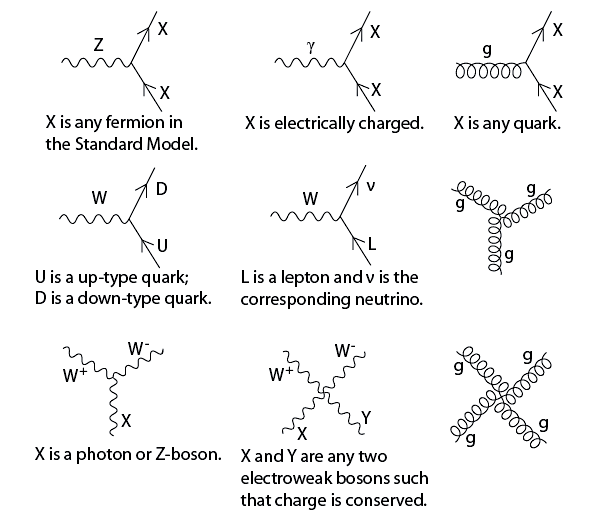
\includegraphics[width=0.84\textwidth]{figures/Standard_Model_Feynman_Diagram_Vertices.png}
	\caption{Feynman diagrams representing the interactions between the fermions and vector gauge bosons in the SM~\cite{SM_interactions}. The charges of the $W$ bosons are determined by conserving charge with the fermions they interact with.}
	\label{fig:SM_interactions}
\end{figure}

\begin{figure}[!htb]
	\centering
	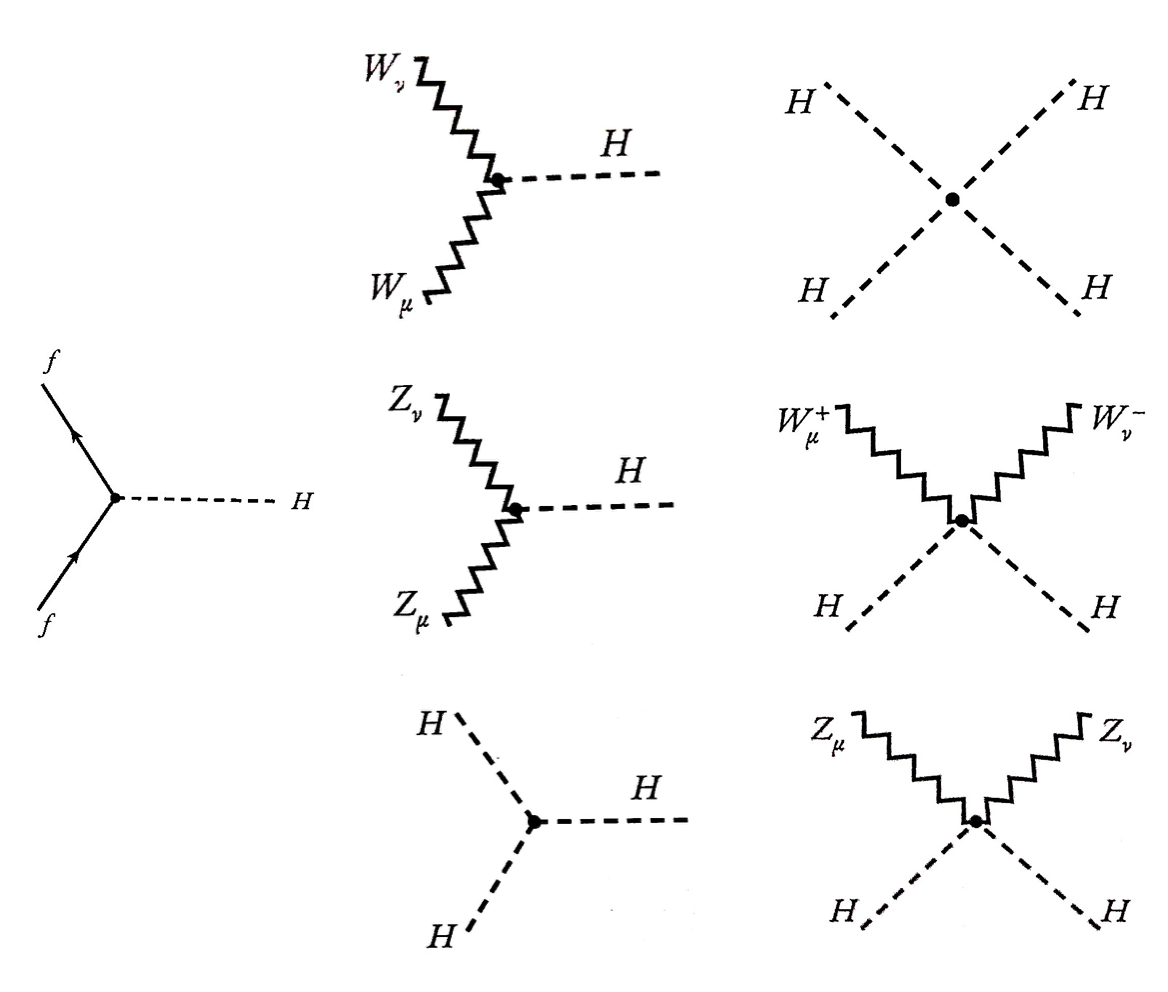
\includegraphics[width=0.75\textwidth]{figures/higgs_sm_couplings.png}
	\caption{Feynman diagrams representing the Higgs boson interactions with the fermions ($f$) and gauge bosons in the SM~\cite{Quigg:2013ufa}.}
	\label{fig:higgs_interactions}
\end{figure}

One mechanism for studying the SM predictions and measuring its free parameters is through particle collisions. At the energy frontier, the SM is currently being probed from proton-proton collisions at the Large Hadron Collider (LHC). Protons are baryons made up of three valence quarks (two $u$ quarks and one $d$ quark), gluons, and sea quarks. Any single proton-proton collision actually involves the interactions among its partons, with the largest momentum transfer occurring in the hard parton-parton collision. The distribution among the partons within the protons is determined from experiment and described by parton distribution functions, which will be used and further discussed in Chapter~\ref{ch:background}. 

The success of the SM can be seen in Fig.~\ref{fig:cms_sm_xsec}, which shows excellent agreement between a wide range of theory and experimental cross section measurements, spanning several orders of magnitude, for the production of various SM processes, as measured by the CMS Collaboration at the LHC. Despite its success, there are several observations not described by the SM. These include a lack of description for dark matter (Section~26, Ref.~\cite{Tanabashi:2018oca}), dark energy (Section~27, Ref.~\cite{Tanabashi:2018oca}), neutrino mass (Section~14, Ref.~\cite{Tanabashi:2018oca}), matter-antimatter asymmetry (Section~21, Ref.~\cite{Tanabashi:2018oca}), vacuum stability (Section~11, Ref.~\cite{Tanabashi:2018oca}), and gravity. In addition, there are several theoretical issues, including no explanation for the large number of free parameters (including why the Yukawa couplings range over six orders of magnitude, or why there are three generations or fermions), no evidence of strong CP violation (Section~13, Ref.~\cite{Tanabashi:2018oca}), no understanding of the origin of gauge group unification, and no solution to the hierarchy problem~\cite{hp1,hp2}. A large number of theories have been developed to solve these issues, such as supersymmetry (Sections~109 and~110, Ref.~\cite{Tanabashi:2018oca}), leptoquarks (Section~115, Ref.~\cite{Tanabashi:2018oca}), and extra-dimensional models (Section~106, Ref.~\cite{Tanabashi:2018oca}). We will investigate the SM hierarchy problem and look at its proposed solution through the addition of extra spatial dimensions in the universe.

\begin{figure}[!htb]
  \centering
  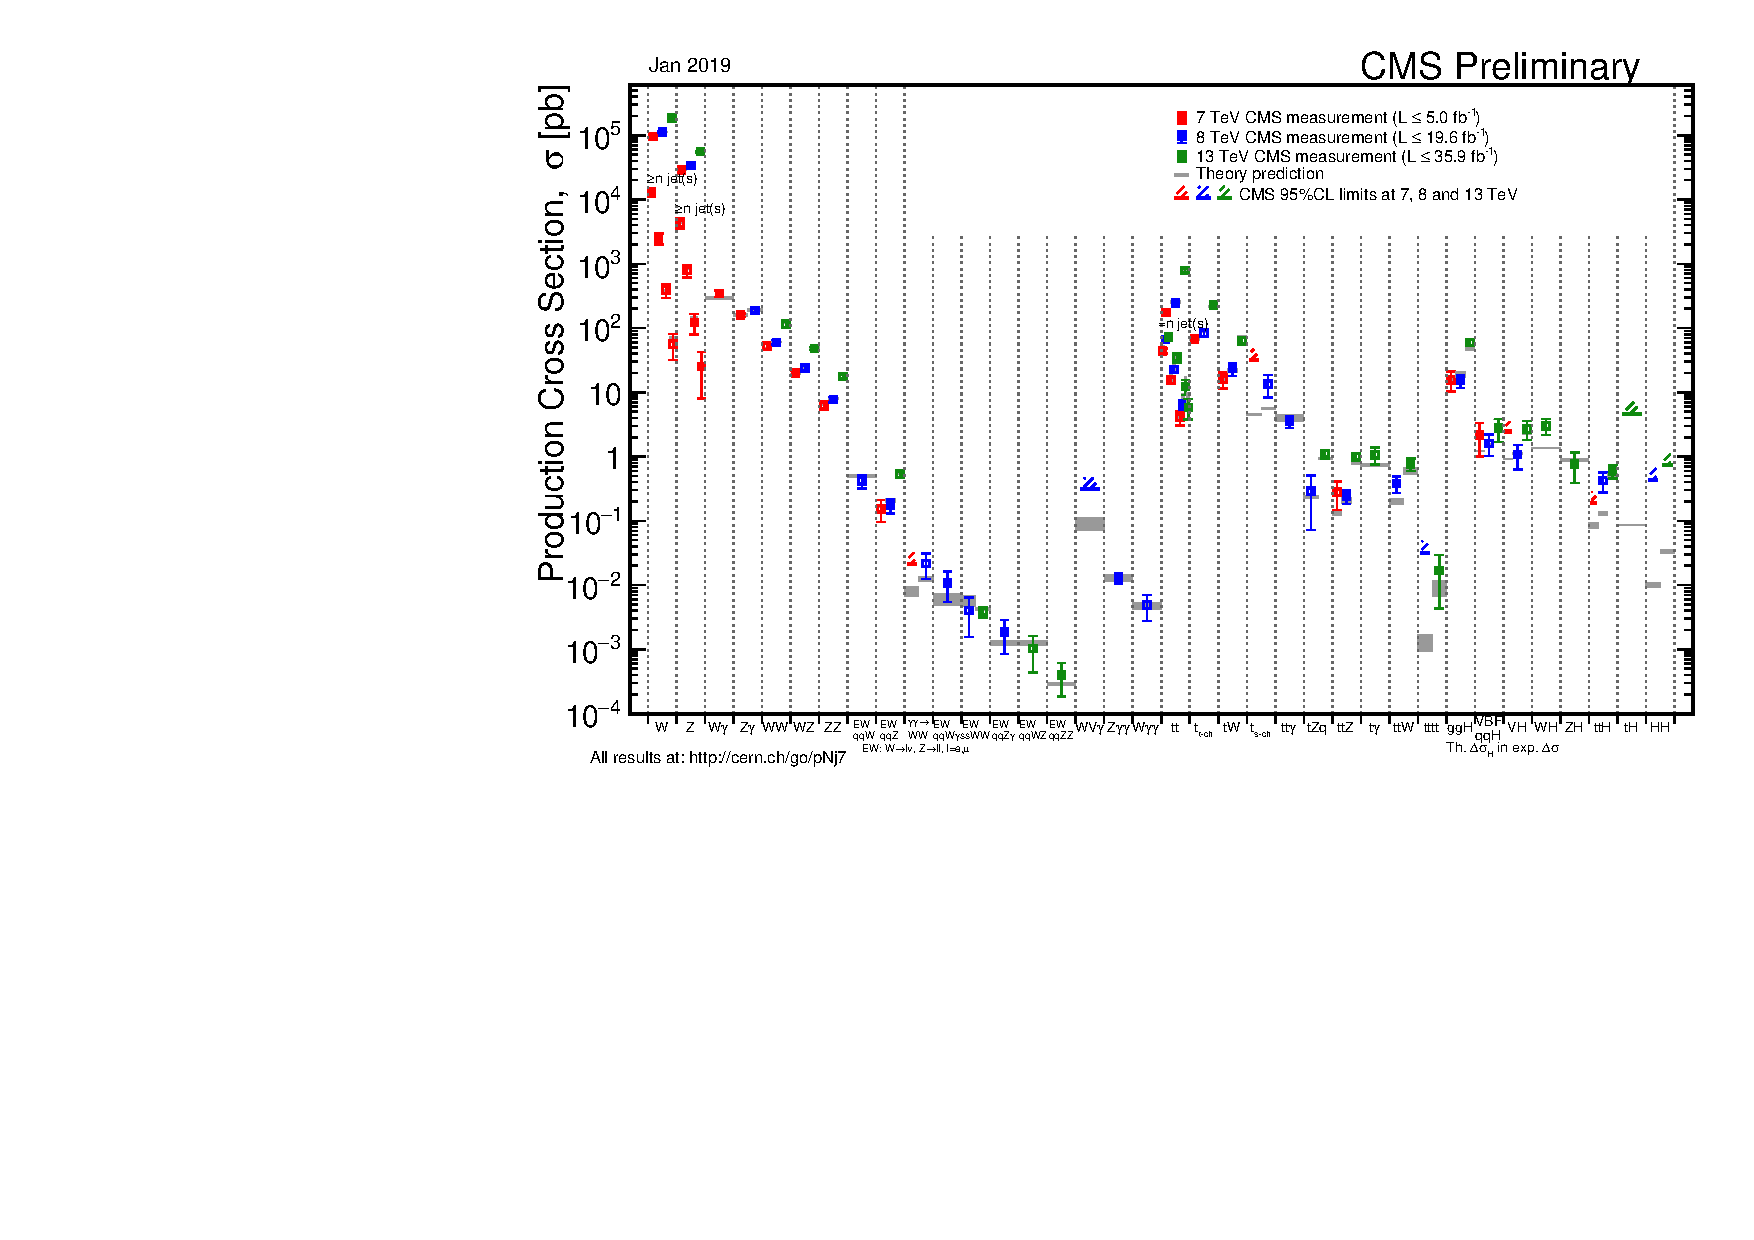
\includegraphics[width=1.0\textwidth]{figures/cms_sm_xsec}
  \caption{Summary of the theory and experimental production cross section measurements of SM processes, measured by the CMS Collaboration~\cite{CMS_xsec}.}
  \label{fig:cms_sm_xsec}
\end{figure}


\section{Beyond the Standard Model}

The shortcomings of the Standard Model suggest that there exists new physics beyond the Standard Model (BSM), offering solutions to its issues. The hierarchy problem, in particular, could be resolved by the existence of extra spatial dimensions in the universe. Among the various extra-dimensional models, the model of large extra dimensions is the focus of this dissertation.

\subsection{Hierarchy Problem}

The hierarchy problem~\cite{hp1,hp2} arises from the large difference between the electroweak scale, $M_{\mathrm{EW}} \sim 10^2\GeV$, and the Planck scale, $\Mpl = (\hbar c/G_{\mathrm{N}})^{1/2} \sim 10^{19}\GeV$, where $G_{\mathrm{N}}$ is Newton's gravitational constant, and has consequences related to the Higgs boson mass $m_H$. Since the Higgs boson is a scalar, coupling to mass, it receives large quantum corrections proportional to $\Lambda^2$ for an ultraviolet cutoff scale $\Lambda$ up to where the theory is valid. This scale arises during the integration of the undetermined momenta of the virtual particles in the loop diagrams associated with the quantum corrections and is used to regulate the loop integrals. Since the Higgs boson is the only scalar in the SM, it is the only SM particle not protected from these corrections. The corrections to the physical Higgs boson mass are of the form
\begin{equation}
	m_H^2 = m_0^2 + \Delta m_H^2
\end{equation}
where $m_0$ is the bare Higgs boson mass and $\Delta m_H^2$ are the mass contributions from the radiative corrections. The one-loop corrections due to a fermion $f$ with Yukawa coupling $y_f$ are given by
\begin{equation}
	m_H^2 \approx m_0^2 - \frac{|y_f|^2}{8\pi^2}\Lambda^2
\end{equation}
The contribution from the $t$ quark is largest with coupling $y_t \sim 1$. The dominant one-loop corrections come from the massive gauge bosons, Higgs boson self-coupling, and the $t$ quark and contribute~\cite{Quigg:2013ufa}
\begin{equation}
	\Delta m_H^2 = \frac{G_F \Lambda^2}{4 \pi^2 \sqrt{2}} (6m_W^2 + 3m_Z^2 + m_H^2 - 12m_t^2)
\end{equation}
where $m_W$, $m_Z$, and $m_t$ are the masses of the $W$ boson, $Z$ boson, and $t$ quark, respectively; and $G_F$ is the Fermi constant, which can be related to each particle's coupling constant. The Feynman diagrams depicting these one-loop corrections are shown in Fig.~\ref{fig:higgs_corrections}.  

\begin{figure}[!htb]
	\centering
	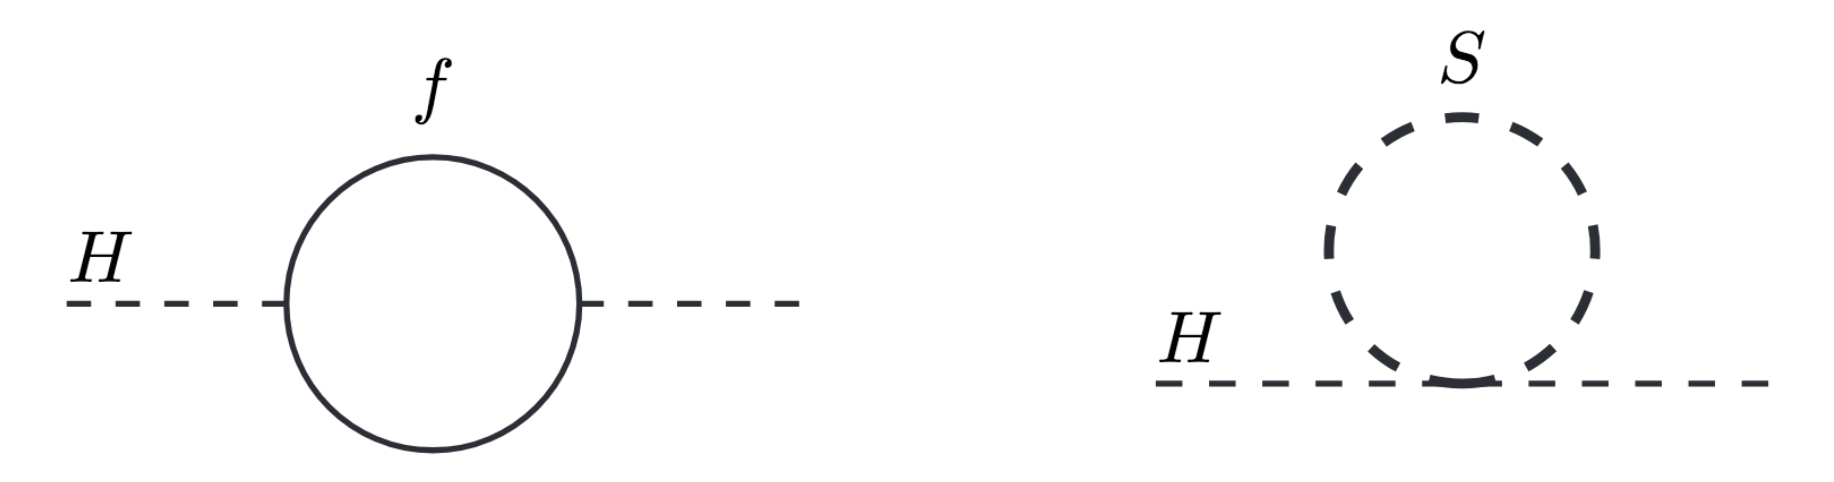
\includegraphics[width=0.75\textwidth]{figures/higgs_corrections.png}
	\caption{One-loop Feynman diagrams for the quantum corrections to the Higgs boson squared mass due to fermions (left) and bosons (right)~\cite{Martin:1997ns}.}
	\label{fig:higgs_corrections}
\end{figure}

The only candidate reference scale for $\Lambda$ is the Planck scale, at which quantum gravity is expected to emerge. Using this scale, the bare mass and the quantum corrections would have to cancel over 30 orders of magnitude in order to arrive at the experimental value of $m_H \simeq 125\GeV$. This extreme degree of cancellation is referred to as fine tuning and seems unnatural. This suggests the possibility of new physics BSM that acts to preserve $m_H$, eliminating the fine tuning requirement. Many models have been proposed. We consider the addition of extra spatial dimensions in the universe as a possible solution, realized through their modification of the fundamental Planck scale.


\subsection{Large Extra Dimensions}

There are several extra-dimensional models that exist since the original idea by Kaluza and Klein~\cite{Kaluza:1921tu,Klein:1926fj,Klein:1926tv}. Among these are the model by Arkani-Hamed, Dimopoulos, and Dvali (ADD)~\cite{ArkaniHamed:1998rs,Antoniadis:1998ig,ArkaniHamed:1998nn}, which proposes flat, large extra dimensions, and the model by Randall and Sundrum~\cite{Randall:1999ee,Randall:1999vf}, which proposes a single, warped extra dimension. A general review of extra-dimensional models and their experimental searches can be found in Section~106 of Ref.~\cite{Tanabashi:2018oca} or in the summary by Hewett and Spiropulu~\cite{Hewett:2002hv}. In general, these models modify the fundamental Planck scale, \MD, such that it can be much lower than the observed Planck scale, \Mpl. In fact, \MD can be on the order of $M_{\mathrm{EW}}$, which would solve the hierarchy problem. Not only could these models solve the hierarchy problem, but establishing the existence of extra dimensions would fundamentally change our picture of the universe.

In the ADD model, the scale of gravity is fundamentally strong, but the gravitational force effectively becomes diluted by the extra spatial dimensions and appears weak to (3\texttt{+}1)-dimensional observers. This is achieved by confining all SM particles and gauge interactions to a (3\texttt{+}1)-dimensional brane embedded in a larger (4\texttt{+}{\nED})-dimensional bulk space with \nED flat extra dimensions assumed to be compactified in a sphere or torus of average radius $R$. Only gravity is free to propagate through the entire bulk space. Following the ideas in Ref.~\cite{ArkaniHamed:1998rs}, Gauss's law in this (4\texttt{+}{\nED})-dimensional space gives the gravitational potential energy between two test masses $m_1$ and $m_2$ separated by a distance $r \ll R$ as
\begin{equation}
	U(r) \sim \frac{m_1m_2}{M_\textrm{D}^{\nED+2}}\frac{1}{r^{\nED+1}}, \; \text{for} \; r \ll R
\end{equation}
If these two masses are placed at distances much larger than $R$, then the usual $1/r$ potential is obtained:
\begin{equation}
	U(r) \sim \frac{m_1m_2}{M_\textrm{D}^{\nED+2}R^{\nED}}\frac{1}{r}, \; \text{for} \; r \gg R
\end{equation}
The effective Planck scale \Mpl is thus
\begin{equation}\label{ADD_size}
	M_{\textrm{Pl}}^2 \sim M_\textrm{D}^{\nED+2}R^{\nED}
\end{equation}

To solve the hierarchy problem, we need $\MD \sim M_{\mathrm{EW}} \sim 1\TeV$. Requiring this in Eq.~(\ref{ADD_size}) yields
\begin{equation}
	R \sim 10^{\frac{30}{\nED}-19}~\text{m}
\end{equation}
Considering values of $\nED=1$, 2, \dots, 7, the corresponding sizes of the extra dimensions for each value are as follows:
\begin{align*}
	\nED &= 1, \quad R \sim 10^{11} \; \text{m}; \\
	\nED &= 2, \quad R \sim 0.1 \; \text{mm}; \\
	\nED &= 3, \quad R \sim 1 \; \text{nm}; \\
	\nED &= 4, \quad R \sim 1 \; \text{pm}; \\
	\nED &= 5, \quad R \sim 100 \; \text{fm}; \\
	\nED &= 6, \quad R \sim 10 \; \text{fm}; \\
	\nED &= 7, \quad R \sim 1 \; \text{fm}.
\end{align*}
These distances are large compared to the characteristic distance scales probed by particle physics interactions, even for $\nED=6$ or 7, corresponding to 10- or 11-dimensions, respectively, which is the number of dimensions suggested by different versions of string theory. \correction{The case for $\nED=1$ would present measurable deviations from Newton's law of gravity, in particular, across solar system distance scales or larger, and can be ruled out.} This is not the case for $\nED \ge 2$. However, tests of Newton's law of gravity at sub-mm distances have started to limit the distance scale for $\nED=2$ and astrophysical and cosmological constraints offer small bounds for $\nED=2$ and 3, as summarized in Section~106 of Ref.~\cite{Tanabashi:2018oca}.


\subsubsection{Phenomenology}

Excitations of the (4\texttt{+}{\nED})-dimensional metric correspond to gravitons. The compactification of the \nED extra dimensions, which have periodic boundary conditions, quantizes the graviton's momentum into different eigenmodes as it propagates along the extra dimensions. From the point of view of a (3\texttt{+}1)-dimensional observer, the eigenmodes appear as a tower of graviton excitations called Kaluza-Klein (\KK) modes. The momentum eigenmodes in (4\texttt{+}{\nED})-dimensions appear as contributions to the mass of each \KK mode in (3\texttt{+}1)-dimensions. The massless graviton propagating in (4\texttt{+}{\nED})-dimensions is equivalent to a massive graviton propagating in (3\texttt{+}1)-dimensions. The mass of excitation $n$ is given by
\begin{equation}
	m_n^2 = m_0^2 + \left( \frac{n}{R} \right)^2
\end{equation}
where $m_0$ is the mass of the ground state \KK mode, corresponding to the fundamental graviton mass in (3\texttt{+}1)-dimensions, which is zero.

Each \KK mode of the graviton (\Gkk) couples to SM particles through the stress-energy tensor with a coupling proportional to $1/M_{\mathrm{pl}}^2$. The couplings are enhanced by the large number of modes that are excited at high energy. These \Gkk modes can decay to SM particles, where they act as propagators in the virtual graviton exchange process. At the LHC, which collides protons, the graviton-mediated processes are initiated through quark annihilation and gluon fusion. The Feynman diagrams depicting these processes with \Gkk decaying to two photons, i.e., $\Gkk \to \gamma\gamma$, are shown in Fig.~\ref{signal_diagrams}.

\begin{figure}[!htb]
	\centering
	
\includegraphics[scale=0.45]{figures/qqToGrav}
	
\includegraphics[scale=0.45]{figures/ggToGrav}
	\caption{Virtual graviton exchange in the diphoton ($\gamma\gamma$) channel through quark annihilation (left) and gluon fusion (right).}
	\label{signal_diagrams}
\end{figure}

The amplitude for any process involving virtual graviton exchange involves a sum over the \KK tower of \Gkk mass states, which can become divergent at high energies, so a cutoff scale needs to be introduced in order to regularize the cross section. Hence, the ADD model is an effective field theory valid only to some cutoff scale $\Lambda_{G}$. This ultraviolet cutoff scale is chosen to be the string scale \Ms~\cite{Han:1998sg}. This procedure results in a higher dimensional operator with coefficients suppressed by some mass scale~\cite{Gleisberg:2003ue}, which can be parametrized by $\etaG = \mathcal{F}/\Ms^4$, where $\mathcal{F}$ is a dimensionless parameter of order unity for which several conventions exist in the literature. We consider the conventions by Giudice, Rattazzi, and Wells (GRW)~\cite{Giudice:1998ck}; Han, Lykken, and Zhang (HLZ)~\cite{Han:1998sg}; and Hewett~\cite{Hewett:1998sn} expressed as:
\begin{equation}
	\label{eqn:add_f_conventions}
	\mathcal{F} = 
	\begin{cases} 
		1 \quad \text{(GRW)}, \\
		\log\left(\frac{\Ms^2}{\hat{s}} \right), \; \text{if} \; \nED = 2 \\ 
		\frac{2}{\nED - 2}, \; \text{if} \; \nED > 2 \\
		\pm\frac{2}{\pi} \quad \text{(Hewett)},
	\end{cases}
	\text{(HLZ)},
\end{equation}
where $\sqrt{\hat{s}}$, in the context of proton-proton collisions at the LHC, is the center-of-mass energy of the hard interaction from the colliding partons. \correction{In the HLZ convention only, $\mathcal{F}$ depends explicitly on \nED and, when $\nED=2$, there is an additional dependence on $\hat{s}$.}

\correction{Considering the interference between the ADD signal and the SM background, the total cross section depends on \etaG according to}
\begin{equation}
	\sigma_{\mathrm{total}} = \sigma_{\mathrm{SM}} + \etaG\, \sigma_{\mathrm{int}} + \etaG^2\, \sigma_{\mathrm{ADD}}
\end{equation}
where $\sigma_{\mathrm{SM}}$ is the cross section of the SM background of the desired processes, $\sigma_{\mathrm{ADD}}$ is the cross section of the pure ADD signal, and $\sigma_{\mathrm{int}}$ is the cross section arising from the interference between the two. The HLZ and GRW conventions interfere constructively, while the Hewett convention can interfere either constructively ($\mathcal{F} = +2/\pi$) or destructively ($\mathcal{F} = -2/\pi$).

For \KK gravitons in the {\TeVns} range, the branching ratios are nearly constant with graviton mass $m_G$ and the total decay width~\cite{Bijnens:2001gh,Tang:2012pv} can be expressed as
\begin{equation}
	\Gamma_{G} \simeq \frac{293m^3_{G}}{960\pi \Lambda^2_{G}}
\end{equation}
The main branching ratios for different SM particles are listed in Table~\ref{tab:grav_BR}. These are dominated by dijet ($gg$ and $q\bar{q}$) production, occurring about 2/3 of the time. Because the $\gamma\gamma$ and $ZZ$ modes contain identical particles, they acquire an additional factor of 1/2, as compared to the distinguishable $W^+W^-$ particles. \correction{The transverse mode of the $Z$ boson provides a contribution to the $ZZ$ branching ratio of the same amount as the $\gamma\gamma$ one; however, its longitudinal mode, acquired through the Higgs mechanism, yields one additional contribution to the $ZZ$ fraction not present for $\gamma\gamma$.} The ratio of the $gg$ to $\gamma\gamma$ branching ratios is 8, since there are 8 gluons but only a single $\gamma$.

\begin{table}[!htb]
	\centering
	\caption{The branching ratios for a massive graviton \Gkk decaying to SM particles with $q=u,d,c,s,b$ and $l=e,\mu$~\cite{Tang:2012pv}. \correction{The remaining 24 modes are split evenly among the 3 flavored neutrino-antineutrino pair and $\tau^+ \tau^-$ decay modes.}}
	\vspace{\baselineskip}
	\cmsTable{
	\begin{tabular}{rcccccccc}
	\hline \hline
	\vspace*{-4.0mm} & & & & & & & & \\
	\Gkk decay mode & $HH$   & $gg$   & $\gamma\gamma$ & $W^+W^-$ & $ZZ$   & $t\bar{t}$ & $q\bar{q}$ & $l^+ l^-$ \\
	Branching ratio &  2/293 & 96/293 & 12/293         & \correction{26/293}   & \correction{13/293} & \correction{18/293}     & 90/293     & 12/293 \vspace*{1.0mm}    \\
	\hline \hline
	\end{tabular}
	}
	\label{tab:grav_BR}
\end{table}

Searching for this ADD signal is favorable in the high-mass diphoton ($\gamma\gamma$) channel. Even though the \KK graviton branching ratio for dijets is dominant among all its decay channels, it suffers from a large background at the LHC. Further, the mass resolution for diphotons is superior to dijets, as provided by the CMS detector at the LHC and discussed in Chapter~\ref{ch:experiment}. Compared to the individual dilepton ($e^+e^-$ or $\mu^+\mu^-$) channels, the branching ratio to diphotons is twice as much. The graviton is a spin-2 particle, so its decay to leptons (spin-1/2) results in a restricted dilepton phase space, while photons are spin-1. Therefore, fermions, unlike photons, cannot be produced in $s$-wave scattering.

In the ADD model, the \Gkk modes are very finely spaced. Since the energy spacing between adjacent modes goes as $1/R$, they range from about 1\meV to about 100\MeV between $\nED=2$-7~\cite{Han:1998sg}. These individual decay modes are too fine to distinguish experimentally, limited by detector resolution. This leads to an effective nonresonant enhancement of the diphoton spectrum at high diphoton invariant mass (\mgg) resulting in a continuum spectrum of diphotons, rather than discrete resonances. Hence, the experimental signature is the nonresonant production of high-mass diphoton objects above the SM diphoton background.

This class of signatures described for the ADD model is by virtual graviton exchange. Since gravity couples to the stress-energy tensor, a graviton can be added to any fundamental SM vertex, e.g., the $s$-channel $q\bar{q}\gamma$ production vertex, allowing a search for direct graviton emission, where a graviton is emitted in the final state, e.g., in $q\bar{q} \to \gamma\Gkk$. These searches depend directly on \MD, and are complementary to the searches by virtual graviton exchange, depending on \Ms, which is expected to be on the order of \MD but may be different from it. An example search for direct graviton emission, as described by the ADD model, in the $\gamma\Gkk$ final state was recently performed by the CMS Collaboration~\cite{Sirunyan:2018dsf}. Interestingly, this model can also be probed by the possibility of microscopic black hole production when the collision energy exceeds \MD~\cite{Banks:1999gd,Dimopoulos:2001hw,Giddings:2001bu}. An example search for microscopic black hole production, as described by the ADD model, by the CMS Collaboration is presented in Ref.~\cite{Sirunyan:2018xwt}. This dissertation searches for signatures of ADD large extra dimensions by virtual graviton exchange in the high-mass diphoton channel using the CMS detector at the LHC.


\subsubsection{Limits on ADD Model Parameters}

No evidence has yet been seen for the existence of extra dimensions, but they have not been ruled out. Previous searches for extra-dimensional signals in the high-mass diphoton channel at collider experiments have been performed by the ATLAS~\cite{ATLAS:2011ab,Aad:2012cy,Aad:2015mna,Aaboud:2016tru,ATLAS-CONF-2016-059,Aaboud:2017yyg}, CMS~\cite{CMS-PAS-EXO-09-004,Chatrchyan:2011jx,Chatrchyan:2011fq,CMS-PAS-EXO-15-004,Khachatryan:2015qba,CMS-PAS-EXO-12-045,Khachatryan:2016yec,Khachatryan:2016hje,Sirunyan:2018wnk}, CDF~\cite{Aaltonen:2011xp}, and D0~\cite{Abazov:2010xh} Collaborations. The searches by the ATLAS and CMS experiments used proton-proton collisions at the LHC with center-of-mass energies $\sqrt{s} = 7,$ 8, and 13\TeV, while those by the CDF and D0 experiments used proton-antiproton collisions at the Tevatron with $\sqrt{s} = 1.96\TeV$. A summary of the extra-dimensional searches by the CMS experiment using $\sqrt{s} = 7$ and 8\TeV is presented by Landsberg in Ref.~\cite{Landsberg:2015pka}.

Searches for large extra dimensions arising from collider signals from virtual graviton effects at the LHC have been performed by the ATLAS and CMS Collaborations in the diphoton~\cite{Aaboud:2017yyg,Sirunyan:2018wnk}, dilepton~\cite{Aad:2014wca,Khachatryan:2014fba}, ditau~\cite{CMS-PAS-EXO-12-046}, and dijet~\cite{Sirunyan:2018wcm} channels. A summary of the corresponding searches in the high-mass diphoton channel by the CMS Collaboration is given in Table~\ref{tab:CMS_ADD_limits}.

% no \Kfactor is applied to the signal
\begin{table}[!htb]
	\centering
	\caption{\correction{A summary of the searches for large extra dimensions in the high-mass diphoton channel performed by the CMS Collaboration's Exotica (EXO) Physics Analysis Group prior to this dissertation.} The 95\% confidence level observed limits on \Ms are given, with the range depending on the model convention.}
	\vspace{\baselineskip}
	\begin{tabular}{cccccc}
	\hline \hline
	\vspace*{-4.5mm} & & & & & \\
	Search       & $\sqrt{s}$ & Data & Year & Limits on \Ms & Ref. \\
	\hline
	%CMS-EXO-09-004 & - & - & - & - & \cite{CMS-PAS-EXO-09-004} \\
	CMS-EXO-10-026 & 7\TeV & 36\pbinv & 2010 & 1.31-2.23\TeV & \cite{Chatrchyan:2011jx} \\
	CMS-EXO-11-038 & 7\TeV & 2.2\fbinv & 2011 & 2.28-3.50\TeV & \cite{Chatrchyan:2011fq} \\
	%CMS-EXO-17-017 & 13\TeV & 35.9\fbinv & 2016 & 5.6-9.7\TeV & \cite{Sirunyan:2018wnk} \\
	\hline \hline
	\end{tabular}
	\label{tab:CMS_ADD_limits}
\end{table}

The current best limits on the ADD model of large extra dimensions arising from collider signals from virtual graviton effects are due to the CMS dijet angular search~\cite{Sirunyan:2018wcm}. This search used data corresponding to 35.9\fbinv with $\sqrt{s} = 13\TeV$. The 95\% confidence level limits on \Ms range between 8.5-12.0\TeV, depending on the model convention. The use of the dijet angular variable provides superior signal sensitivity than simply considering only the dijet invariant mass. In the diphoton channel, ATLAS sets 95\% confidence level limits on \Ms between 5.7-8.1\TeV using 37\fbinv with $\sqrt{s} = 13\TeV$~\cite{Aaboud:2017yyg}. This dissertation searches in the CMS high-mass diphoton channel using 35.9\fbinv with $\sqrt{s} = 13\TeV$~\cite{Sirunyan:2018wnk} and aims to extend these results.


\section{Organization of Dissertation}

The remainder of this dissertation is organized as follows. \correction{The experimental apparatus used in this large-extra dimensional search is the combination of the LHC and CMS detector}, as described in Chapter~\ref{ch:experiment}. Event reconstruction and selection within the CMS detector, with an emphasis on photon reconstruction and diphoton selection, are detailed in Chapter~\ref{ch:event_selection}. Chapter~\ref{ch:background} presents the background determination for this nonresonant diphoton search. The ADD large extra-dimensional signal is simulated according to the methods of Chapter~\ref{ch:signal}. Sources of systematic uncertainty are discussed in Chapter~\ref{ch:systematics}, and the results are presented in Chapter~\ref{ch:results}.




\hypersetup{pageanchor=true}

\chapter{Experimental Apparatus}\label{ch:experiment}

\section{Large Hadron Collider}

The Large Hadron Collider (LHC)~\cite{Evans:2008zzb} is a superconducting synchrotron that accelerates two counter-rotating, circular beams of hadrons and collides them at four interaction points (IPs) where experiments are placed, as depicted in Fig.~\ref{lhc-overview}. It is operated by the European Organization for Nuclear Research (CERN), which is headquartered in Geneva, Switzerland, and is their flagship experiment. \correction{The LHC is installed in the 26.7~km circumference tunnel that was used by the CERN Large Electron-Positron collider and lies beneath the France-Switzerland border at depths as low as 175~m below the surface.} It accelerates separate beams of protons (p) or lead ions (Pb) yielding pp, pPb, or PbPb collisions. The LHC primarily operates using pp collisions. Operation for production physics began in 2010. In October 2017, xenon (Xe) beams were successfully tested and XeXe collisions were achieved. 

\begin{figure}[!htb]
	\centering
	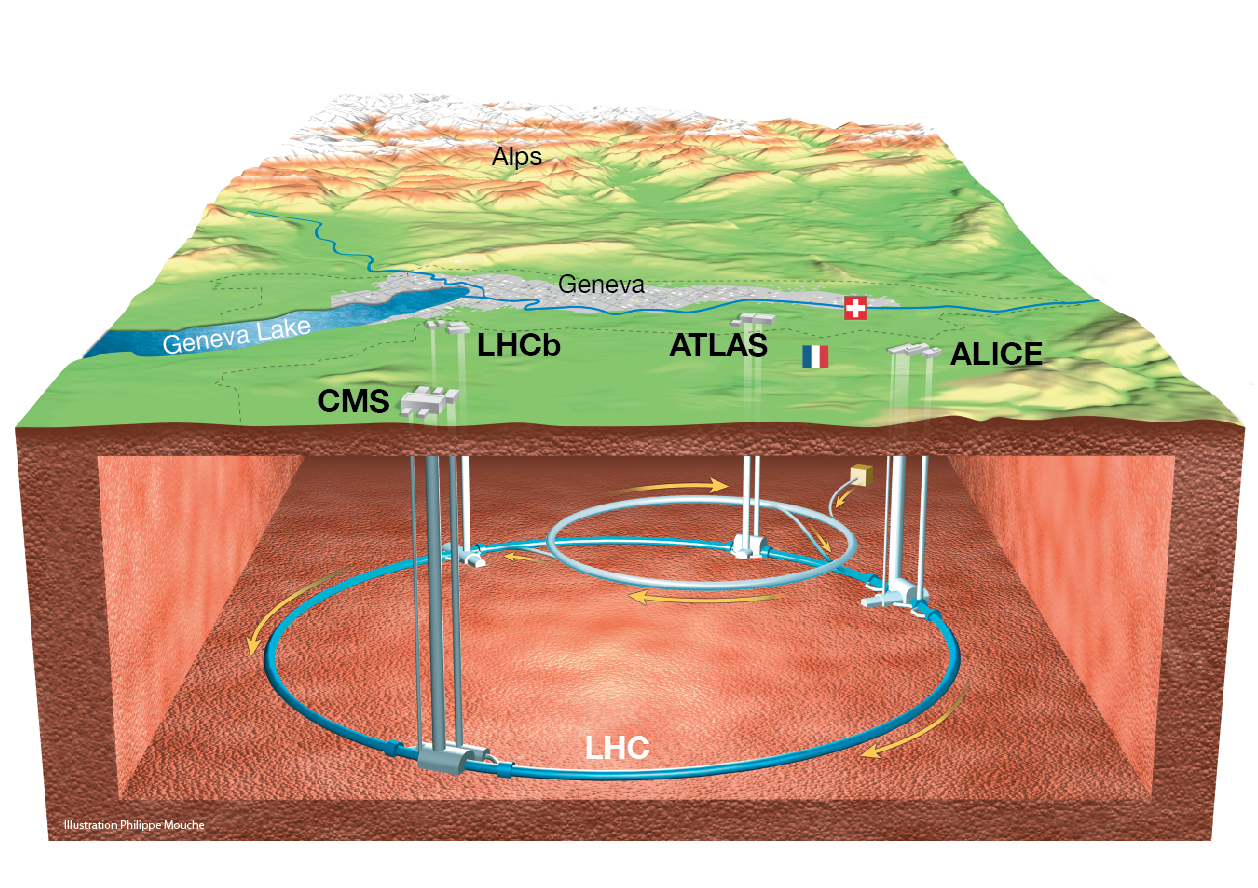
\includegraphics[scale=0.25]{figures/lhc_overview}
	\caption{An overview of the location of LHC and its four interaction points~\cite{Mouche:1708847}.}
	\label{lhc-overview}
\end{figure}

\subsection{The CERN Accelerator Complex}

The LHC is designed to achieve pp collisions at a center-of-mass energy $\sqrt{s} = 14\TeV$. Protons are delivered to the LHC after going through a series of stages in the CERN accelerator complex, as shown in Fig.~\ref{accelerator-complex}. During each stage, the proton's energy is steadily increased using older accelerators from the previous generations of CERN experiments.  

\begin{figure}[!htb]
	\centering
	\includegraphics[width=1.0\textwidth]{figures/CCC-v2018-print-v2.pdf}
	\caption{The CERN accelerator complex~\cite{Mobs:2636343}.}
	\label{accelerator-complex}
\end{figure}

Protons are sourced from a bottle of hydrogen gas which is ionized using electric fields. After ionization, the electrons are separated and the protons that are left behind are initially accelerated to 50\MeV using the Linac~2 linear accelerator. The beam is then sent to the circular Proton Synchrotron Booster where it reaches an energy of 1.4\GeV before being injected into the circular Proton Synchrotron and further accelerated to 25\GeV. Next, the beam is transferred to the nearly 7~km circumference Super Proton Synchrotron which accelerates the beam to an energy of 450\GeV. The protons are finally injected into the LHC where they reach their final center-of-mass energy of up to 14\TeV. After acceleration, the two counter-rotating beams are brought together and the protons are collided at the four IPs where detectors are placed.

\begin{figure}[!htb]
	\centering
	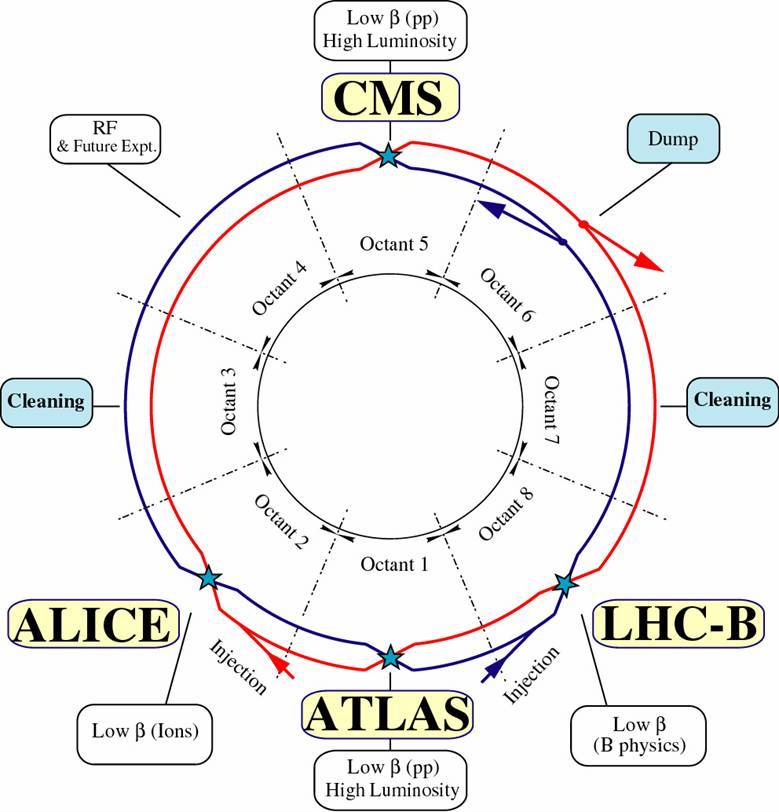
\includegraphics[scale=0.40]{figures/lhc-interaction-points}
	\caption{A schematic of the eight LHC insertion points~\cite{LHC_schematic}.}
	\label{lhc-ips}
\end{figure}

The LHC has insertions at its Points~1, 2, 5, and 8 housing the IPs where the respective ATLAS~\cite{Aad:2008zzm}, ALICE~\cite{Aamodt:2008zz}, CMS~\cite{Chatrchyan:2008aa}, and LHCb~\cite{Alves:2008zz} experiments are located. ATLAS and CMS are general purpose collider detectors designed to search for and study the Higgs boson, perform precision measurements of SM parameters, study strongly interacting matter, and search for evidence of physics beyond the SM. LHCb is designed to study heavy flavor physics, primarily searching for evidence of new physics in CP violation from beauty and charm hadron decays. ALICE is a general purpose heavy ion detector designed to study the physics of strongly interacting matter and the quark-gluon plasma. In addition to these four major LHC experiments, four more insertion points are used for LHC operations. Point 4 contains radio frequency (RF) cavities inserted to accelerate the particle beams. The insertions in Points~3 and 7 host collimators used for beam cleaning, and Point~6 contains the beam dump insertion. Fig.~\ref{lhc-ips} shows a schematic of the eight LHC insertion points, which includes the four IPs.


\subsection{The LHC Components}

The LHC uses RF cavities to accelerate the particle beams. Superconducting dipole electromagnets are used to bend the beams and quadrupole magnets are used for focusing. \correction{There are 1232 dipole and 392 quadrupole magnets around the LHC ring, each 15~m and 3~m long, respectively.} The dipole magnets are constructed using NbTi superconducting coils capable of generating an 8.3~T magnetic field. \correction{A cross-section of a dipole magnet is depicted in Fig.~\ref{lhc-dipole}.}

\begin{figure}[!htb]
	\centering
	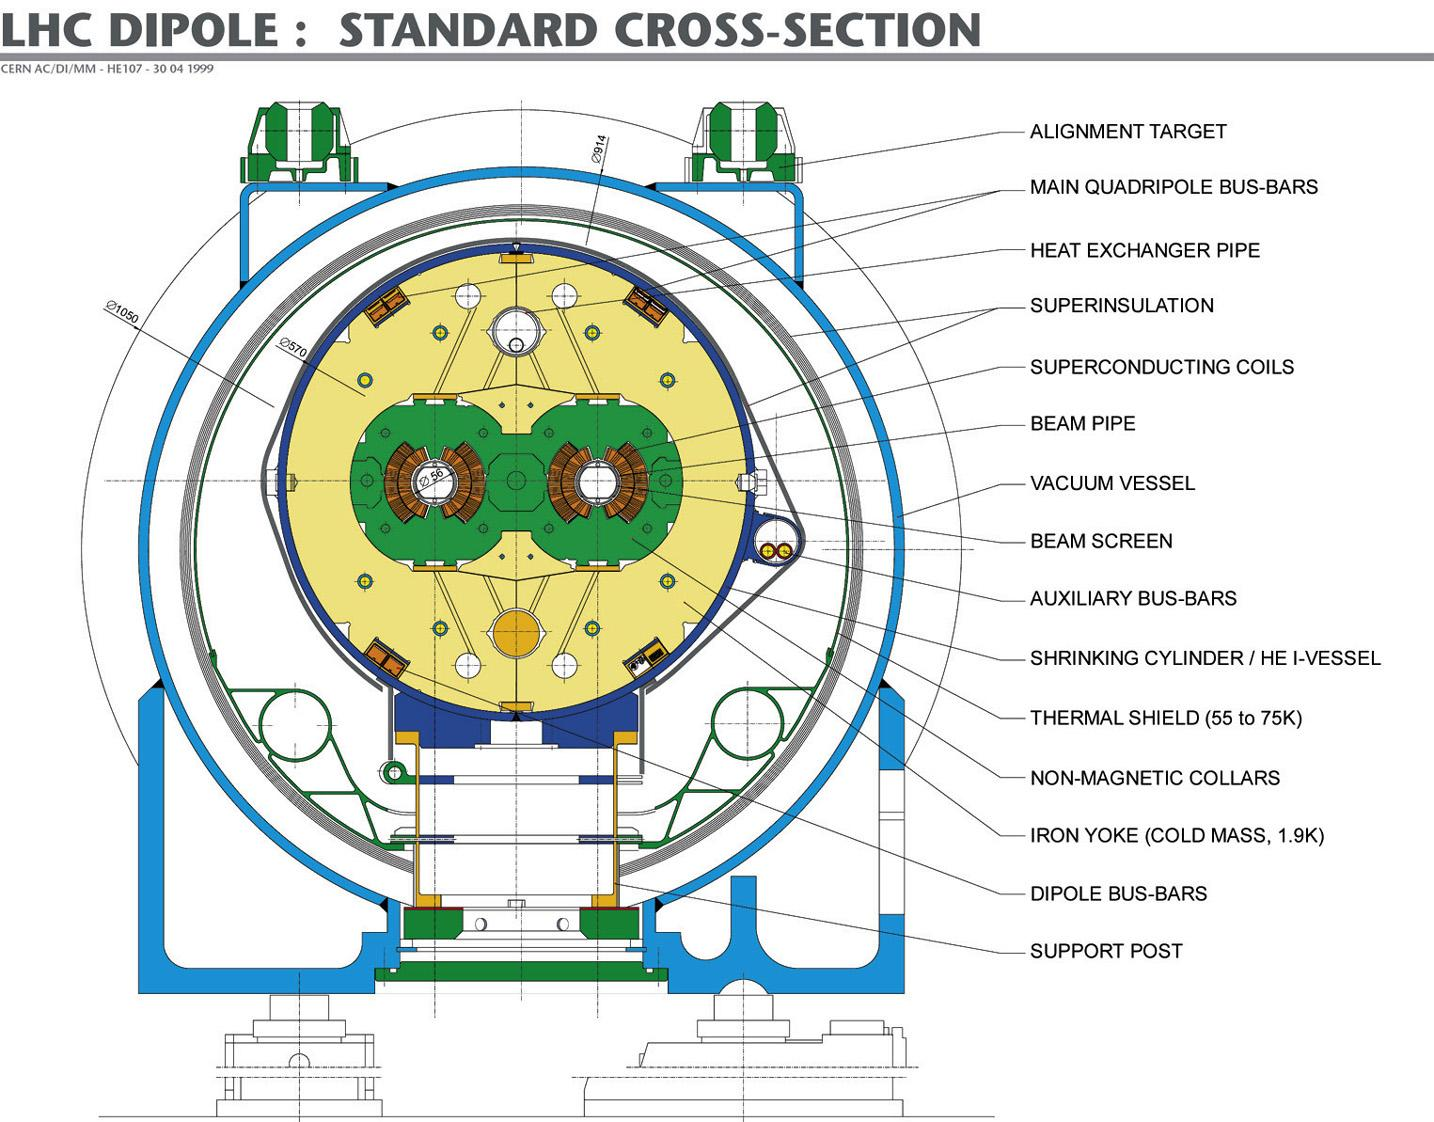
\includegraphics[scale=0.50]{figures/lhc_dipole}
	\caption{A cross-section of an LHC dipole magnet~\cite{Team:40524}.}
	\label{lhc-dipole}
\end{figure}

The proton beams are divided into bunches containing on the order of $10^{11}$~protons/bunch. At designed operation, bunches are spaced so that they occur 25~ns apart. Given the LHC orbit length of $89.1~\mu$s, a maximum of 3564 bunches are possible in each beam. Bunches are injected in the LHC in bunch trains separated by empty bunches which allow for beam monitoring, calibration, and control. At nominal operation, 2808 bunches are filled in each beam. The total number of events $N$ produced in the collisions are related to the integrated luminosity $L$ of the LHC fill by
\begin{equation}
	L = N\sigma
\end{equation}
where $\sigma$ is the proton-proton interaction cross section. The total proton-proton cross section at $\sqrt{s} = 14\TeV$ is expected to be roughly 100~mb~\cite{Bruning:782076}. At $\sqrt{s} = 13\TeV$, CMS measured the inelastic portion of this cross section to be approximately 70~mb in a restricted phase space of the detector~\cite{Sirunyan:2018nqx}. The integrated luminosity is calculated from the instantaneous luminosity $\mathcal{L}$ by the anticipated relation $L = \int \mathcal{L} \, \text{d}t$. The instantaneous luminosity is determined from the beam parameters by
\begin{equation}
	\mathcal{L} = \frac{N_{\mathrm{b}}^2 f n_{\mathrm{b}}}{4\pi\sigma_{\mathrm{x}}^*\sigma_{\mathrm{y}}^*}F
\end{equation}
where $N_{\mathrm{b}}$ is the number of protons/bunch, or beam intensity; $n_{\mathrm{b}}$ is the number of bunches; $f = 11.2455$~kHz is the LHC revolution frequency; $\sigma_{\mathrm{x,y}}^*$ are the transverse RMS beam widths at the IP; and $F$ is a geometric loss factor used to correct for the beam crossing angle, shape, and longitudinal beam size. For a Gaussian beam at nominal LHC operation, both $\sigma_{\mathrm{x}}^*$ and $\sigma_{\mathrm{y}}^*$ equal $16.6~\mu$m. The loss factor is about 0.83~\cite{Bruning:782076}. The instantaneous luminosity is not constant throughout the period of duration during stable beam collisions. This is primarily due to beam intensity degradation and emittance growth. The luminosity decays with a lifetime $\tau$ according to
\begin{equation}
	\mathcal{L} = \mathcal{L}_0e^{-t/\tau}
\end{equation}
where $\mathcal{L}_0$ is the peak instantaneous luminosity, which, at nominal pp LHC operation, is on the order of $10^{34} \;\text{cm}^{\texttt{-}2} \, \text{s}^{\texttt{-}1}$. A snapshot of the LHC status display, taken during pp collisions, is given in Fig.~\ref{fig:lhc_fill_decay}, showing the decay in instantaneous luminosity over time as measured by the LHC experiments. The lifetime during stable beam collisions is about 20~hours. However, during typical operation, stable beams can be lost to electrical trips or contamination in the beam pipe.

\begin{figure}[!htb]
	\centering
	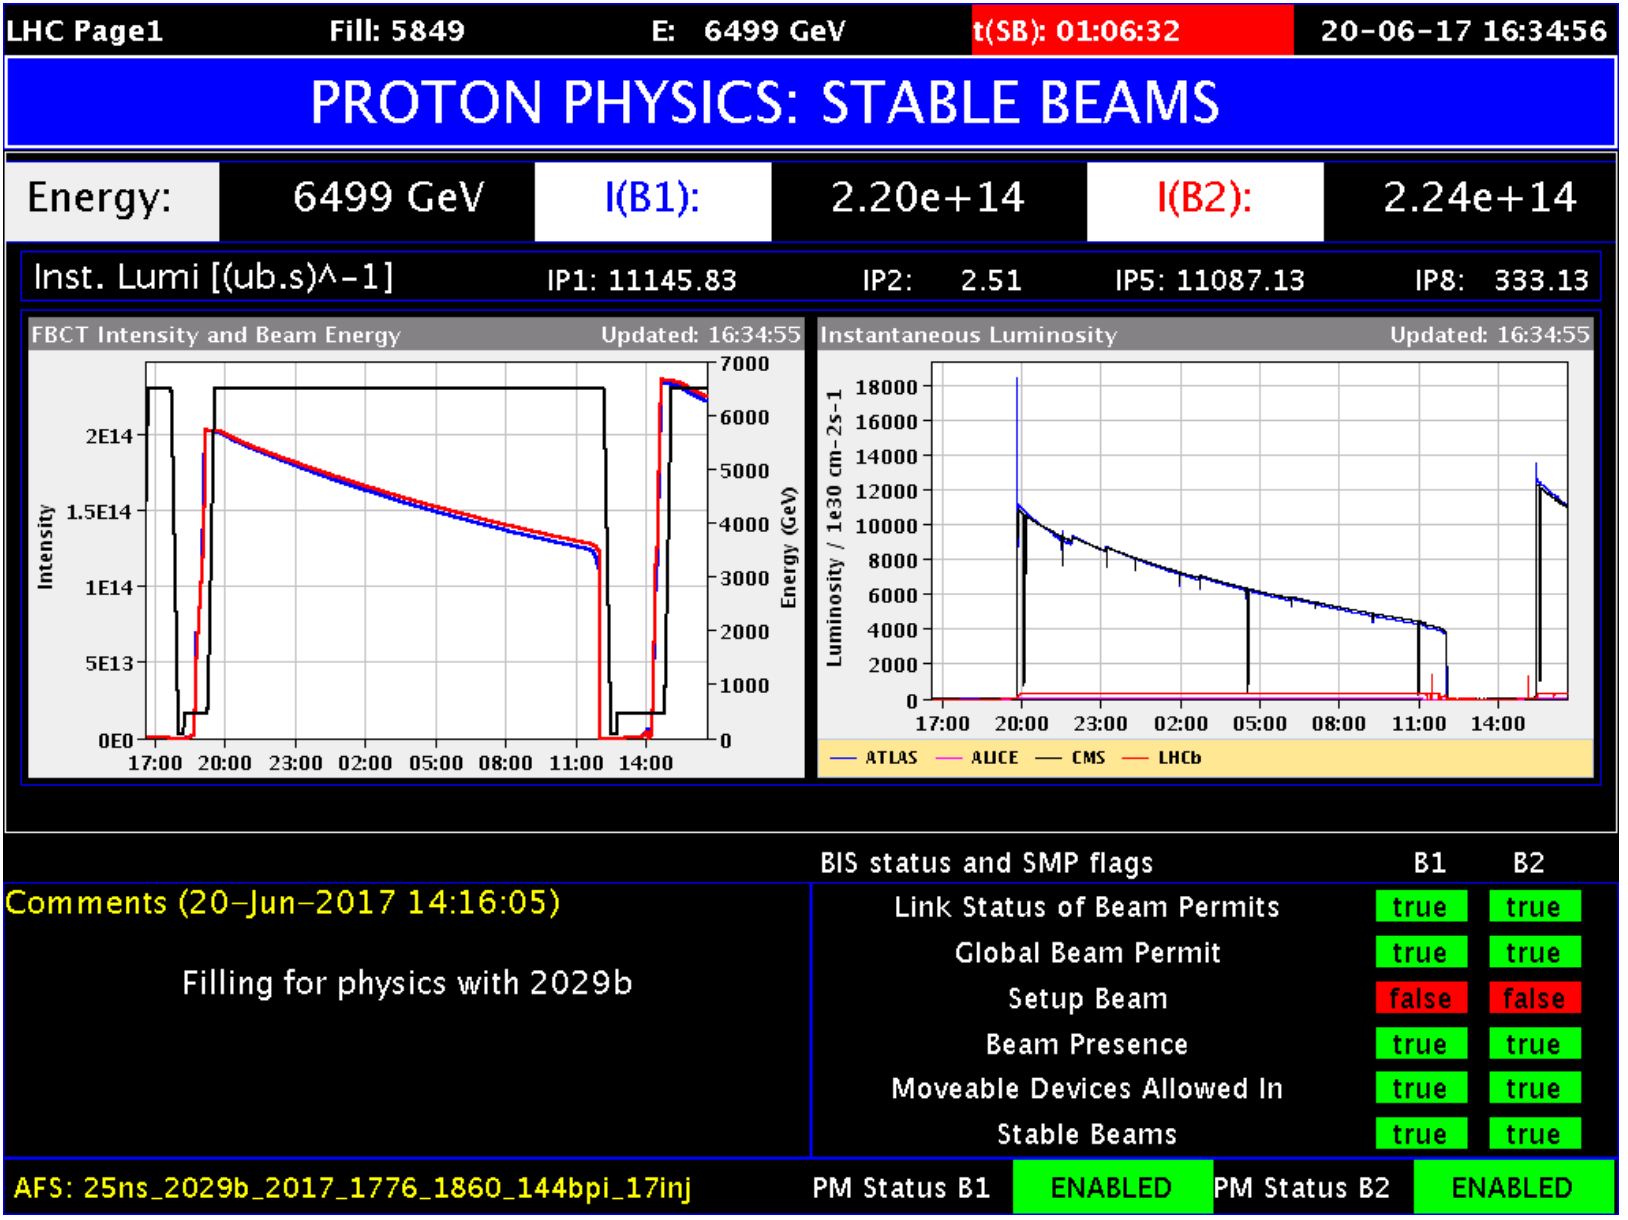
\includegraphics[width=0.80\textwidth]{figures/lhc_fill_decay}
	\caption{A snapshot of the LHC status display, taken in June 2017 during stable beam pp physics collisions, showing the decay in instantaneous luminosity over time as measured by the LHC experiments.}
	\label{fig:lhc_fill_decay}
\end{figure}


\subsection{The LHC Schedule}

The LHC operates during production cycles known as Runs, which typically last for 3-4~years. During any year within an LHC running period, stable proton-proton collisions used for production physics are only performed for part of that year. For the other part of that year, the LHC is shutdown for about 3-4~months to accommodate upgrades and repairs and additional running time is allocated for beam commissioning, special requests by the experiments for beam use, and heavy ion collisions. Runs are followed by an extended period of accelerator inactivity without beams known as a Long Shutdown (LS). During this time, major upgrades and repairs are performed on the accelerator and each of its experiments. The first pp collisions were achieved in November 2009 and physics production began in March 2010, marking the start of the Run~1 LHC physics program. The current planned longterm LHC schedule is summarized in Table~\ref{tab:LHC_schedule}.

\begin{table}[htbp!]
	\caption{A summary of the current planned longterm LHC schedule. A tentative schedule extends past LS3.}
	\label{tab:LHC_schedule}
	\centering
  \vspace{\baselineskip}
	\begin{tabular}{ll}
	\hline \hline
	LHC period & Duration \\
	\hline
	Run 1 & 2010-2012 \\
	LS1   & 2013-2014 \\
	Run 2 & 2015-2018 \\
	LS2   & 2019-2020 \\
	Run 3 & 2021-2023 \\
	LS3   & 2024- \\
	\hline \hline
	\end{tabular}
\end{table}

During the first part of Run~1 from 2010-2011, the LHC performed pp collisions at $\sqrt{s} = 7\TeV$. In 2010, the LHC delivered an integrated luminosity of 44.9\pbinv, of which 41.5\pbinv were recorded by CMS. In 2011, this increased to 6.1\fbinv being delivered and 5.6\fbinv recorded. The collision energy for pp collisions was increased to $\sqrt{s} = 8\TeV$ during the second part of Run~1 beginning in 2012. This resulted in the LHC providing an integrated luminosity of 23.3\fbinv, of which CMS recorded 21.8\fbinv and certified 19.7\fbinv for physics analysis use. During Run~1, a 50~ns bunch spacing was used.

Starting with Run~2, the collision energy was further increased to $\sqrt{s} = 13\TeV$. During the first two months of physics data taking, a 50~ns bunch spacing was used, but, in August 2015, this spacing was reduced to the nominal LHC value of 25~ns, where it remains. In 2015, the LHC delivered 4.2\fbinv with 3.8\fbinv of it recorded by CMS. This increased as the LHC delivered an integrated luminosity of 40.8\fbinv to CMS in 2016 and 49.8\fbinv in 2017, of which 37.8\fbinv and 45\fbinv was recorded, respectively. \correction{In 2018, 68.2\fbinv were delivered by the LHC and 64\fbinv were recorded by the CMS detector, using the current best offline data reconstruction. Future improvements in the offline reconstruction could change the final numbers. This marks the end of Run~2. In total, 163\fbinv were delivered by the LHC and 150.5\fbinv were recorded by CMS with 139.7\fbinv being certified for physics analysis use in Run~2. During Runs~1 and~2, a combined integrated luminosity of approximately 192.5\fbinv were delivered by the LHC to the CMS detector.} A summary of this during each year of Runs~1 and~2 is shown in Fig.~\ref{fig:lumi_cms}. Also shown is a detailed breakdown for 2016, which is the year the dataset used by the analysis in this dissertation was recorded. For more information on the CMS luminosity measurement in 2016, see Ref.~\cite{CMS-PAS-LUM-17-001}.

A major goal during LS2 is to prepare the LHC for reaching its nominal collision energy of $\sqrt{s} = 14\TeV$, planned for Run~3 operation. By the end of Run~3, it is expected that many of the LHC components will suffer severe radiation damage and will need to be replaced. Therefore, at the start of LS3, the LHC is planned to be upgraded to the High-Luminosity Large Hadron Collider (HL-LHC)~\cite{Apollinari:2284929}. The HL-LHC is being designed to integrate ten times more luminosity than the LHC. This high luminosity environment poses significant challenges to the LHC experiments and will require them to undergo major changes, especially in the forward region of the detectors. To accommodate this, the CMS Collaboration, in particular, is preparing for its Phase II upgrade~\cite{Contardo:2020886,Butler:2055167}, which includes a proposal to replace its existing endcap calorimeters with a high granularity calorimeter~\cite{Collaboration:2293646}. 

\begin{figure}[!htbp]
	\centering
	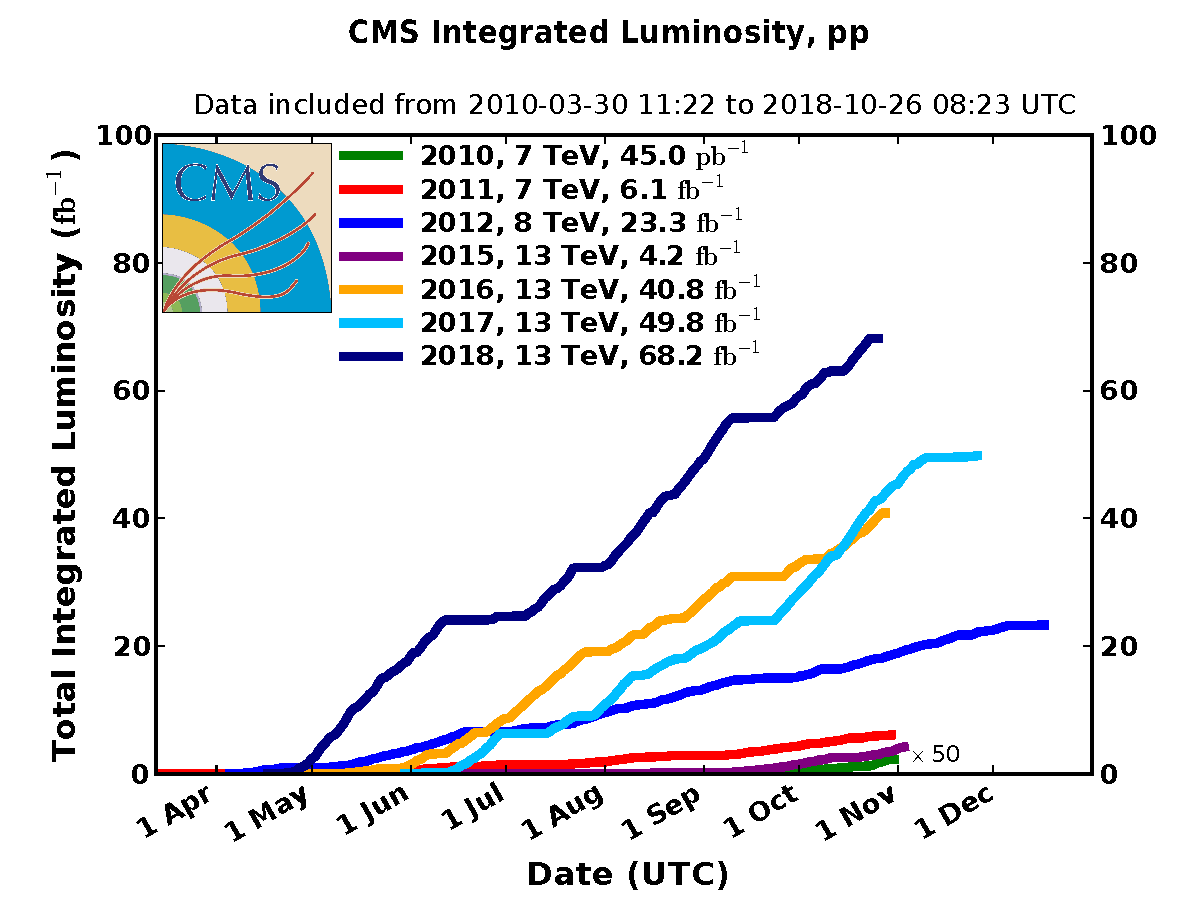
\includegraphics[scale=0.40]{figures/int_lumi_cumulative_pp_2.pdf}
	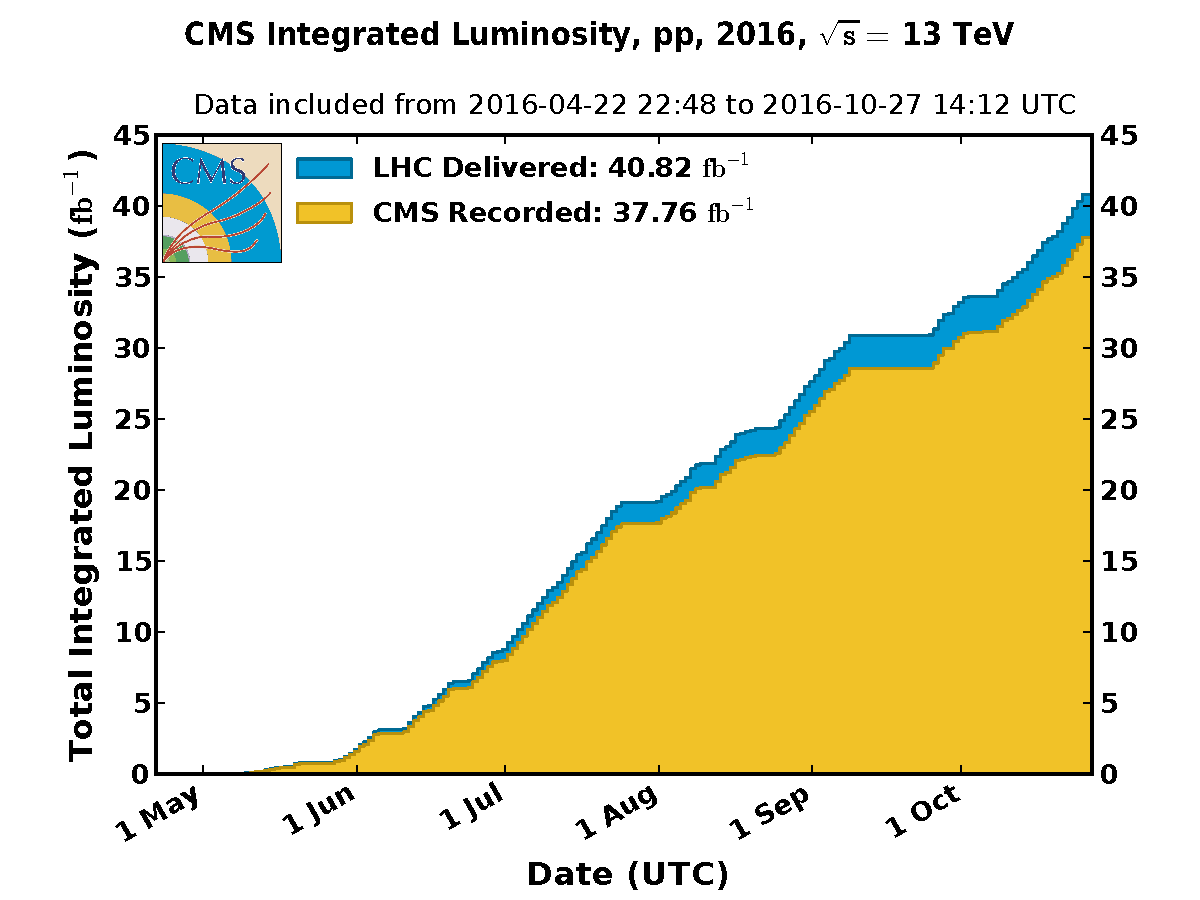
\includegraphics[scale=0.40]{figures/int_lumi_per_day_cumulative_pp_2016.pdf}
	\caption{A timeline showing the cumulative (left) and detailed 2016 (right) integrated luminosity delivered by the LHC~\cite{CMS_lumi}. The amount recorded by CMS in 2016 is also shown.}
	\label{fig:lumi_cms}
\end{figure}


\section{The CMS Detector}

The Compact Muon Solenoid (CMS) detector~\cite{Chatrchyan:2008aa} is a general purpose particle physics experiment designed for high performance in the search for the Higgs boson and for BSM physics at the {\TeVns} scale. It operates as one of the LHC experiments located underground at Point~5 of the LHC ring located in Cessy, France. The overall detector has a cylindrical form approximately 15~m in diameter and 28.7~m in length, weighing about \correction{14000 metric tons}. A defining feature of CMS is its 6~m internal diameter superconducting solenoid, providing a uniform magnetic field of 3.8~T inside the majority of its detector volume. CMS comprises several subdetectors arranged in a barrel and endcap configuration, centered on the beam axis, consisting of an inner silicon pixel and strip tracking system; a crystal electromagnetic calorimeter (ECAL); a brass and scintillator hadron calorimeter (HCAL), all of which are mostly contained inside of the solenoid; and gas ionization muon chambers embedded in the steel return yoke of the solenoid. Fig.~\ref{CMS} depicts a 3D cutaway model of the CMS detector, highlighting its major components in this configuration.

\begin{figure}[!htb]
	\centering
	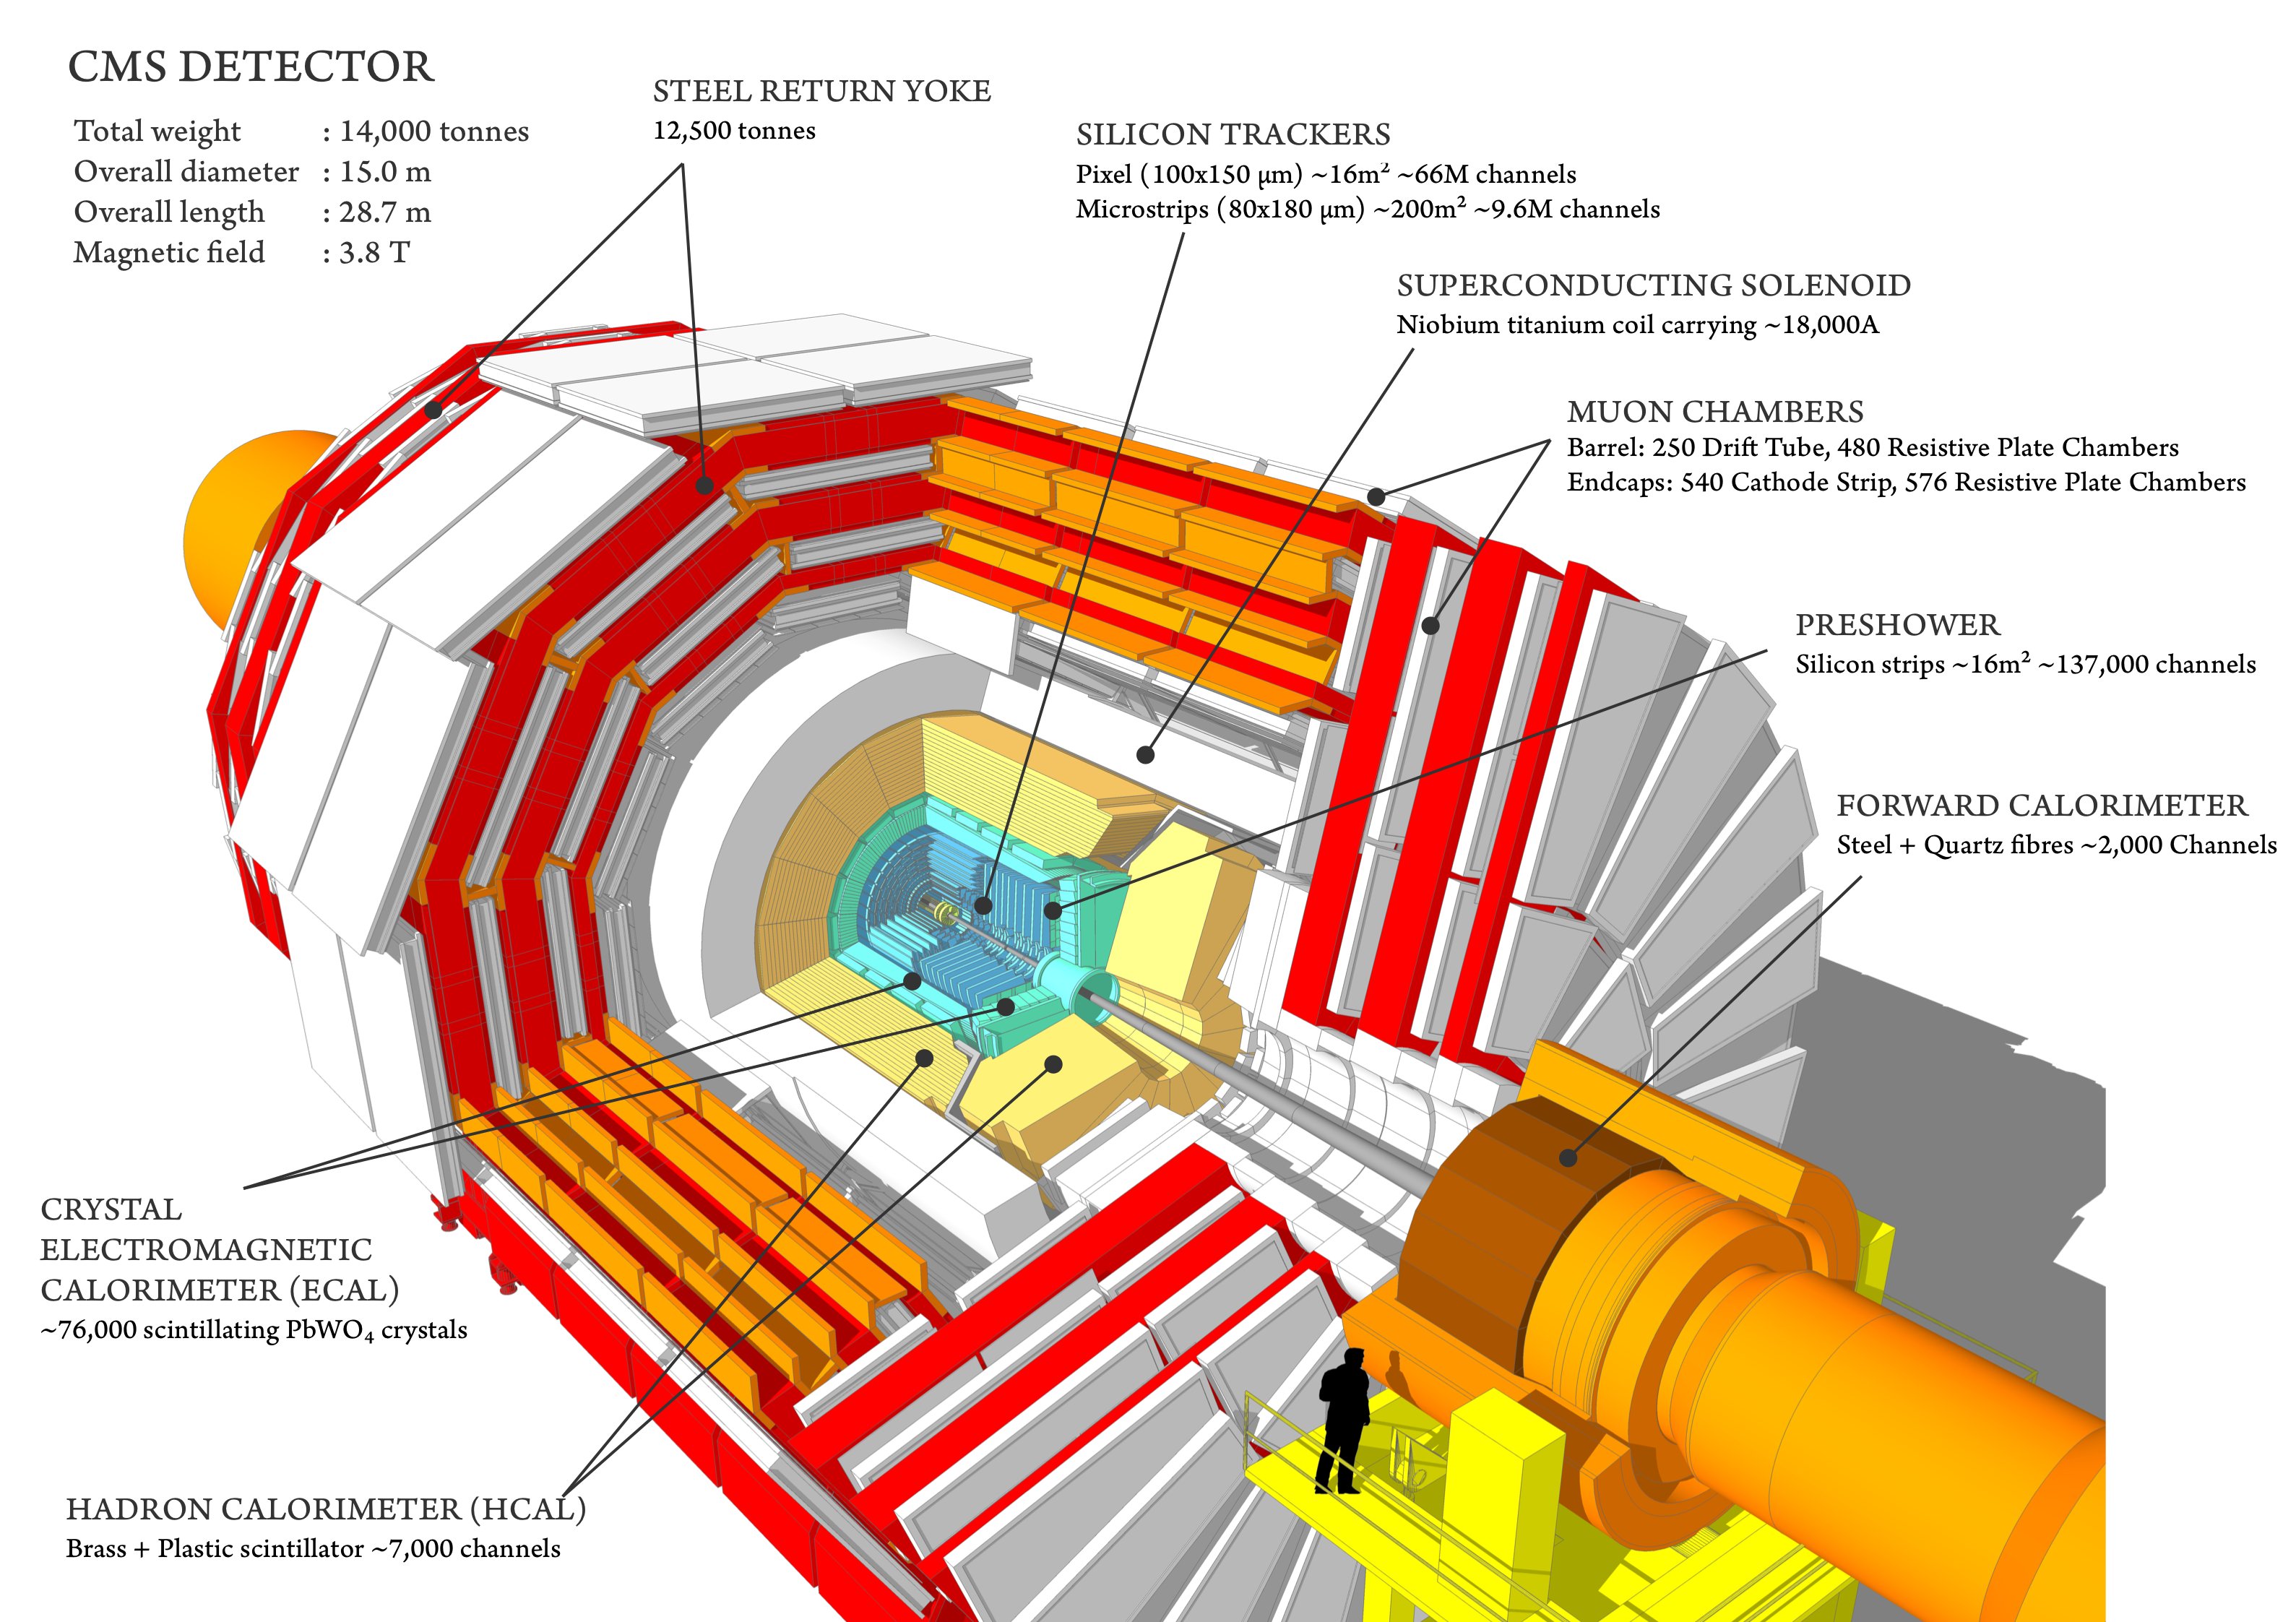
\includegraphics[width=1.0\textwidth]{figures/cms_sketchup}
	\caption{An overview of the CMS detector and its major components~\cite{Sakuma:2013jqa}.}
	\label{CMS}
\end{figure}

Particle detection in CMS relies on information from each subdetector, starting with the inner most detectors. Different particles interact differently with the various detector technologies, possibly leaving behind tracks or energy deposits in different regions, as depicted in Fig.~\ref{cms-slice}. This information is read out using a sophisticated trigger and data acquisition system, consisting of the detector electronics, Level-1 trigger, readout network, and high-level trigger. After describing the CMS coordinate system, we will discuss each of its major components.

\begin{figure}[!htbp]
	\centering
	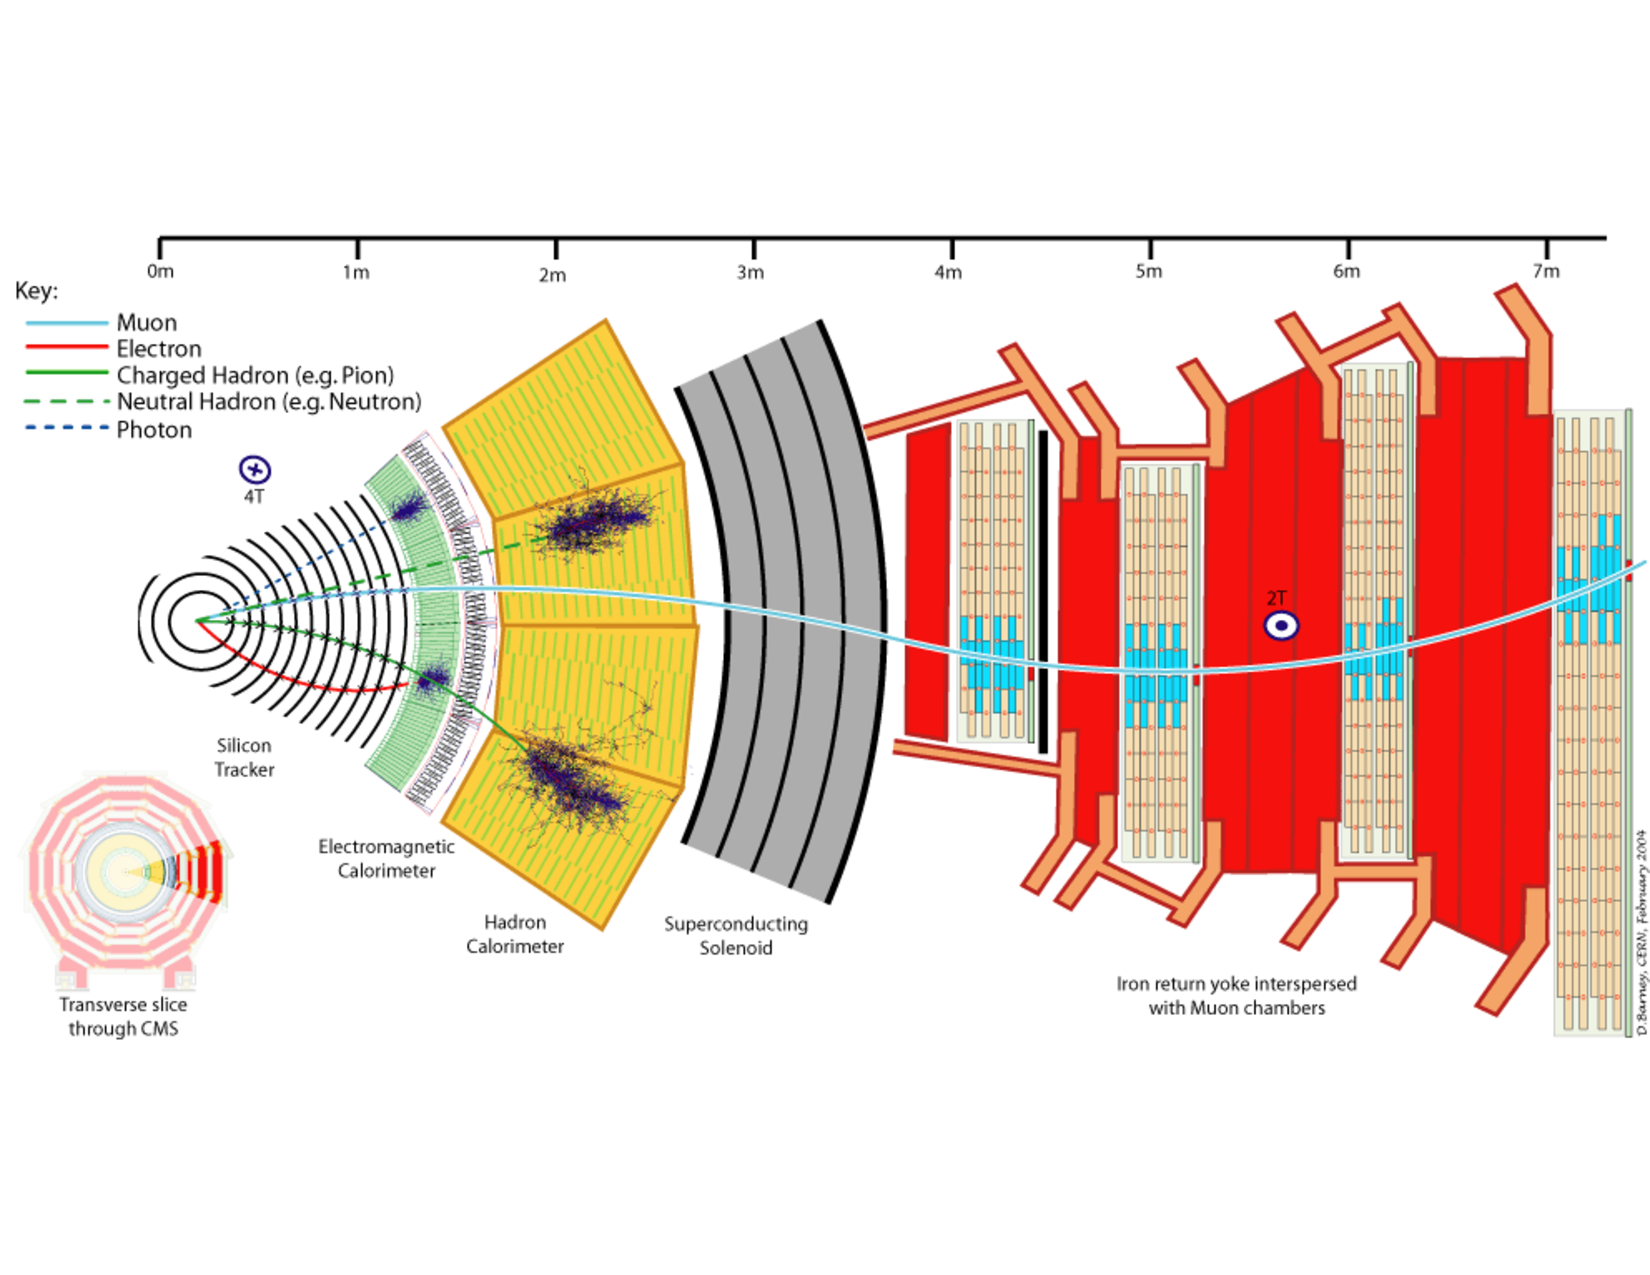
\includegraphics[width=1.0\textwidth]{figures/CMS_slice.pdf}
	\caption{A transverse slice of the CMS detector highlighting how different particles interact with its various detector technologies~\cite{Davis:2205172}.}
	\label{cms-slice}
\end{figure}


\subsection{Coordinate System}

CMS uses a right-handed coordinate system with its origin located at the nominal LHC interaction point inside of the detector. The $x$-axis points inward towards the center of the LHC, the $y$-axis points vertically upward perpendicular to the LHC plane, and the $z$-axis points along the direction of the counterclockwise rotating beam. Due to its geometry, cylindrical coordinates of the form $(z,\theta,\phi)$ are used. The azimuthal angle $\phi$ is measured from the $x$-axis in the transverse $x$-$y$ plane, and the polar angle $\theta$ is measured from the $z$-axis. A diagram illustrating both the Cartesian and cylindrical coordinate systems is shown in Fig.~\ref{fig:coordinate_system}. 

\begin{figure}[!htb]
	\centering
	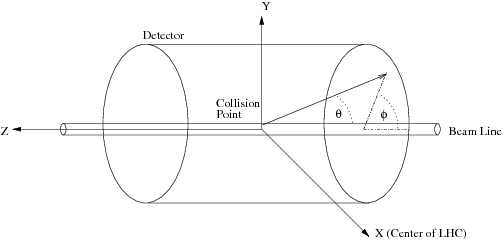
\includegraphics[scale=0.75]{figures/coordinate_system.png}
	\caption{An illustration of the coordinate system used by the CMS detector~\cite{Schott:1699952}.}
	\label{fig:coordinate_system}
\end{figure}

Measurements of particle energy $E$ and momentum $p$ in the transverse plane are denoted $E_{\mathrm{T}} = E \sin\theta$ and $\pt = p \sin\theta$, respectively. Typically, the pseudorapidity, defined as $\eta = - \ln[\tan(\theta/2)]$, is preferred to $\theta$. Particle coordinates are often expressed as $(\pt, \eta, \phi)$, with distances in the $\eta$-$\phi$ plane given by $\Delta R = \sqrt{(\Delta\phi)^2 + (\Delta\eta)^2}$.


\subsection{Inner Tracking System}

The inner tracking system of CMS is designed to measure the trajectories of charged particles emerging from the collisions, as well as perform the reconstruction of secondary vertices, such as from $b$ quark and $\tau$ lepton decays. This system consists of the silicon pixel and strip tracker subdetectors, laid out according to Fig.~\ref{fig:tracker}.

\begin{figure}[!htb]
	\centering
	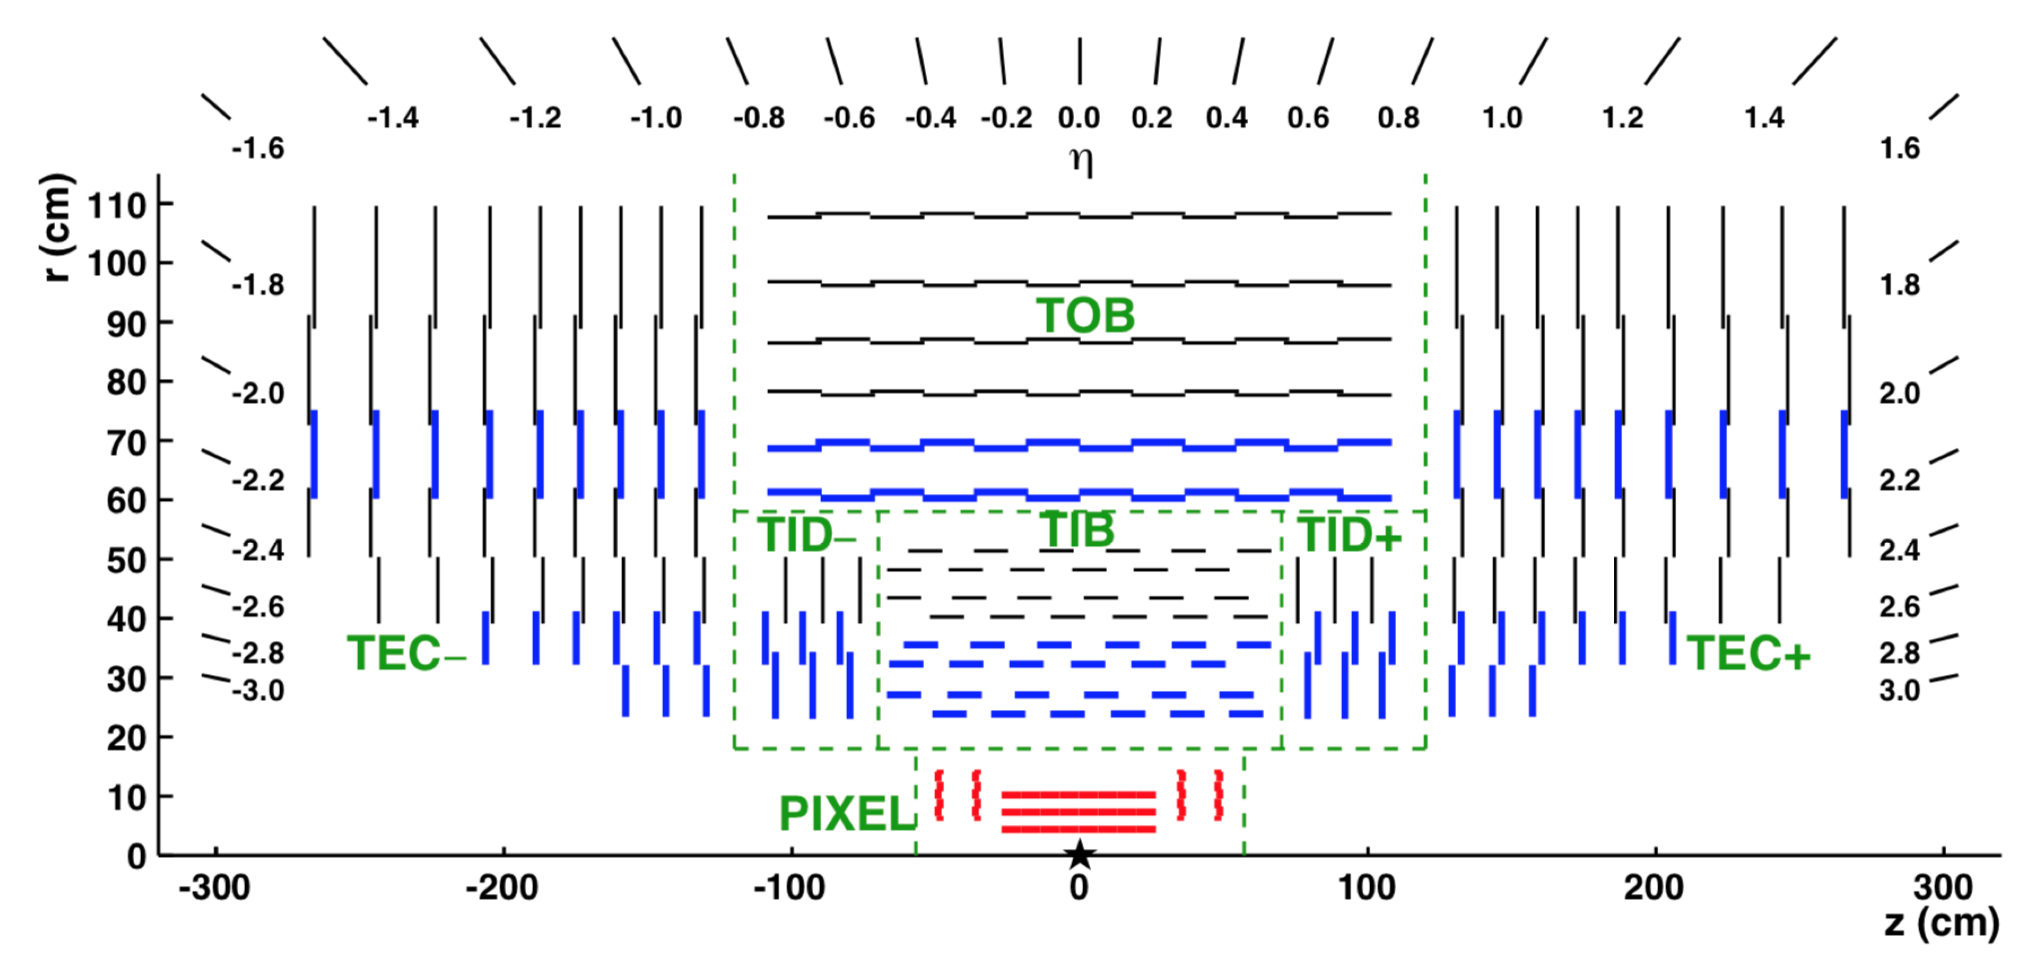
\includegraphics[width=0.85\textwidth]{figures/inner_tracker.png}
	\caption{A schematic of the CMS inner tracking system~\cite{Sirunyan:2018icq}.}
	\label{fig:tracker}
\end{figure}

The silicon pixel detector consists of 3 barrel layers (BPix) and 2 endcap disks (FPix), which surround the interaction point, providing coverage in the range $-2.5<\eta<2.5$. The BPix layers are 53~cm long and located at radii of 4.4, 7.3, and 10.2~cm. The FPix are placed at $z=\pm34.5$ and $\pm46.5$~cm with radii ranging from 6-15~cm. A single silicon pixel cell has an area of $100{\times}150$~$\mu$m. In total, the BPix (FPix) consists of 48 (18) million pixels covering an area of 0.78 (0.28)~$\textrm{m}^2$.

The silicon strip tracker consists of four subsystems: the tracker inner barrel (TIB), tracker inner disks (TIDs), tracker outer barrel (TOB), and tracker endcaps (TECs). Both the TIB and TIDs are located out to $r=55$~cm and comprise 320~$\mu$m thick silicon microstrip sensors arranged in 4 barrel layers and 3 disks, respectively. This inner barrel and disk system is surrounded by the TOB, which has an outer radius of 116~cm and extends between $z=\pm118$~cm. The TOB consists of 6 barrel layers of 500~$\mu$m thick silicon microstrip sensors. The TECs cover the range $124<|z|<282$~cm, surrounding the rest of the system. Each TEC comprises 9 disks with radii ranging between 22.5-113.5~cm, using silicon strips either 320 or 500~$\mu$m thick. The entire strip tracker has a total of 9.3 million silicon strips covering a total area of 198~$\textrm{m}^2$.

The performance of the inner tracking system is presented in Ref.~\cite{Chatrchyan:2014fea}, and the reconstruction of tracks and vertices is discussed in Section~\ref{sec:event_reco}.


\subsection{Electromagnetic Calorimeter}\label{sec:ECAL}

The electromagnetic calorimeter (ECAL) is designed to detect and measure the energy of electrons and photons. The ECAL is a hermetic, homogeneous calorimeter comprising approximately 75000 lead tungstate (PbW$\text{O}_4$) scintillating crystals separated into a barrel (EB) and two endcap (EE) sections, which give coverage up to $|\eta|<3.0$. These crystals were chosen for their high granularity, short radiation length, high radiation tolerance, and fast response time. Avalanche photodiodes are used to detect the scintillation light in the EB and vacuum phototriodes are used in the EEs. The scintillation light is caused by high-energy electrons or photons initiating an electromagnetic shower in the crystals. This occurs for electrons when they undergo bremsstrahlung until their energy loss becomes dominated by ionization and for photons when they undergo pair production until their energies fall below the pair production threshold. The electromagnetic shower ionizes the atoms in the crystals and light is emitted when they de-excite. The amount of light produced is proportional to the energy of the incident particles. A general description of the passage of particles through matter and, in particular, their detection using calorimeters is given in Sections~33 and~34 of Ref.~\cite{Tanabashi:2018oca}.

The EB is located at $y = 1.29$~m and covers the range $|\eta| < 1.479$. It is made up of 61200 crystals constructed into 36 identical supermodules, each covering half of the barrel length. Each supermodule is made up of 4 modules, and these modules are made up of various submodules each containing 2 rows of 5 crystals. The gap between adjacent crystals is 320~$\mu$m. A single crystal in the EB covers an area of about $22{\times}22$~m$\text{m}^2$ in $\eta$-$\phi$, giving a granularity of $\Delta\eta{\times}\Delta\phi = 0.0174{\times}0.0174$. Each crystal is of length 230~mm, corresponding to 25.8 radiation lengths ($X_0$). The crystals are tilted at $3^{\circ}$ with respect to the origin in both the $\eta$ and $\phi$ directions, allowing for the detection of particles that would otherwise travel between the gaps of the crystals.


Each EE is located at $z = \pm 3.14$~m and covers the range $1.479 < |\eta| < 3.0$. They are made up of a total of 14648 crystals. Both are divided into two half-disk arrangements constructed with crystals tapered in an $x$-$y$ grid, grouped into $5{\times}5$ structures called supercrystals. A single crystal in an EE covers an area of about $28.6{\times}28.6$~m$\text{m}^2$ in $x$-$y$ and is of length 220~mm, corresponding to 24.7~$X_0$. The gap between adjacent crystals is 320~$\mu$m and between different $5{\times}5$ units is 2~mm.

A preshower detector (ES) is placed in front of each EE in the region $1.653 < |\eta| < 2.6$. These are primarily used to help distinguish between photons and $\pi^0$ decays which mimic a single photon signature. The ES is a sampling calorimeter made of 2 disks of lead and 2 planes of silicon strip detectors, providing about 3~$X_0$ of material. A cutaway view of the ECAL highlighting its main features is shown in Fig.~\ref{ecal}.

\begin{figure}[!htb]
	\centering
	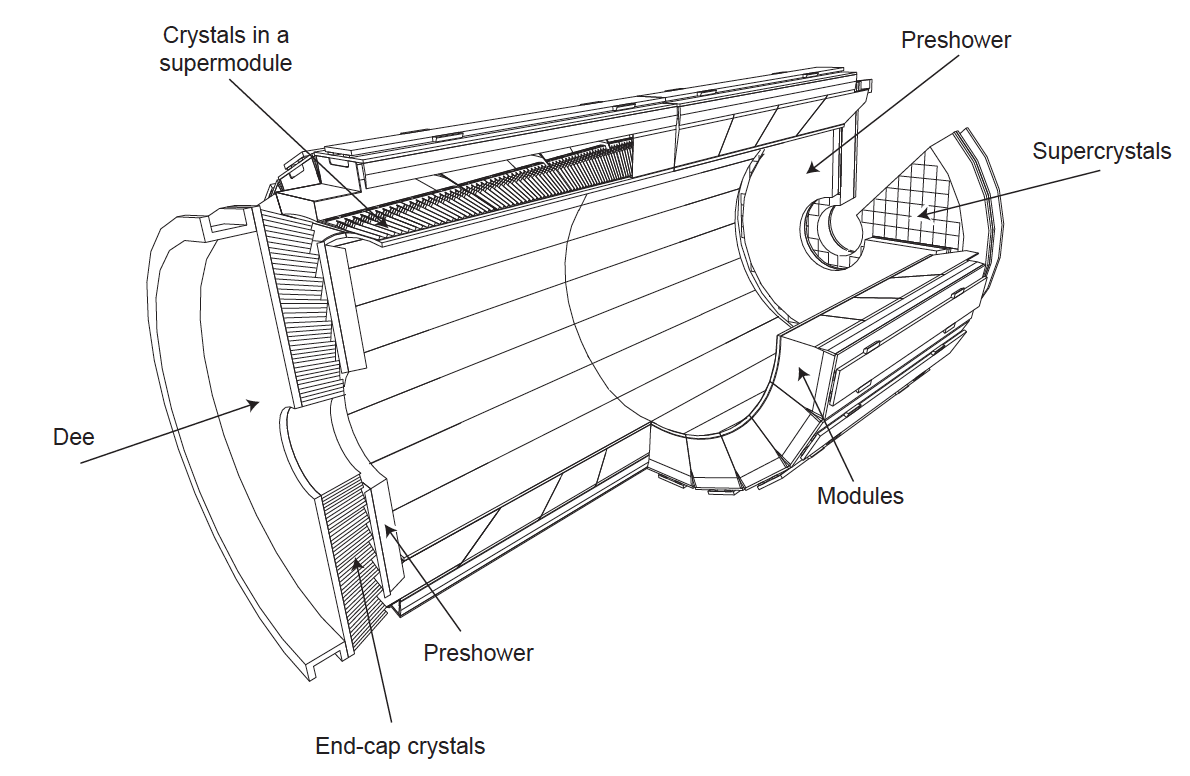
\includegraphics[scale=0.55]{figures/ecal}
	\caption{A cutaway view of the ECAL depicting its main features~\cite{Chatrchyan:2008aa}.}
	\label{ecal}
\end{figure}

The ECAL uses an active laser monitoring system to measure the relative response of laser light injected into the crystals. \correction{The response degrades over time as high radiation doses are received, with limited recovery during periods without collisions, as shown in Fig.~\ref{ecal_laser}.} These measurements are performed every 40 minutes and are used to correct the physics data. 

\begin{figure}[!htb]
	\centering
	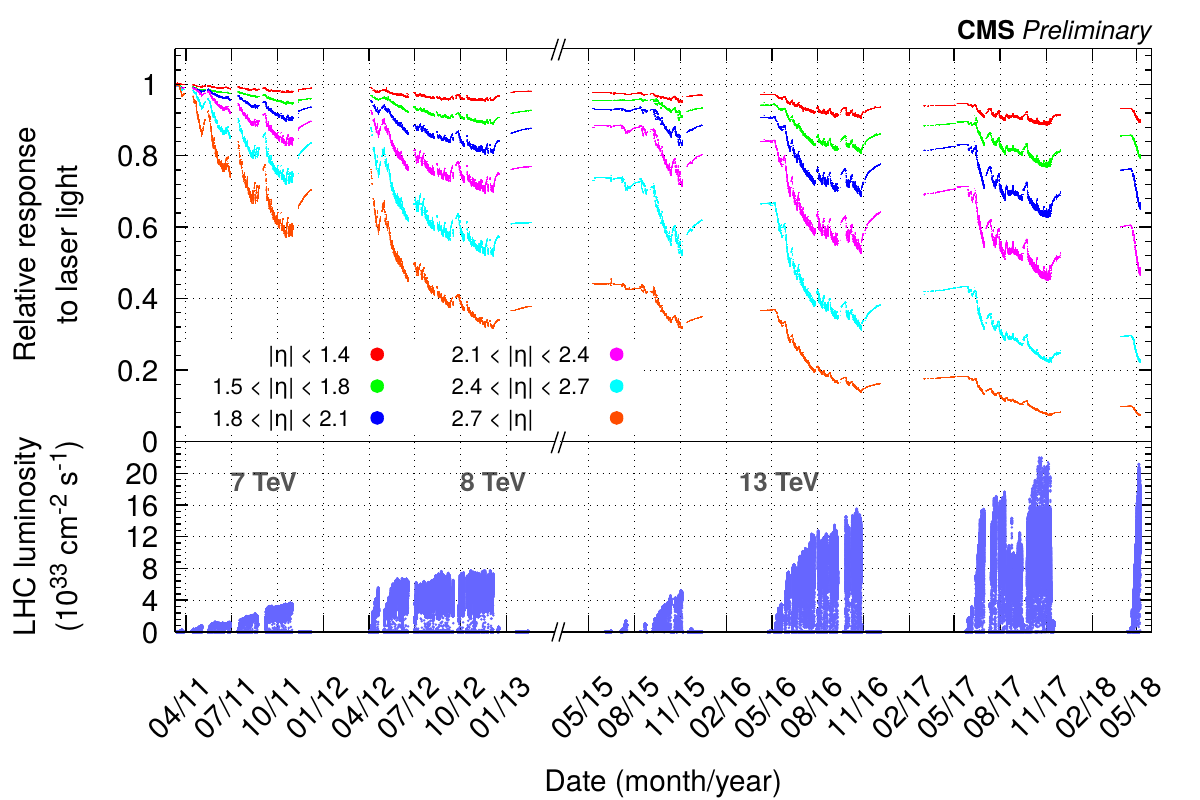
\includegraphics[width=0.85\textwidth]{figures/ecal_laser}
	\caption{The ECAL crystal response measured by the ECAL laser monitoring system over the LHC data taking periods~\cite{CMS-DP-2018-015}.}
	\label{ecal_laser}
\end{figure}

The energy resolution of the ECAL as a function of energy $E$ is characterized by separate terms added in quadrature of the form
\begin{equation}
	\frac{\sigma_E}{E} = \frac{a}{\sqrt{E}}\,\oplus\,\frac{b}{E}\,\oplus\,c
\end{equation}
for a stochastic term $a$, a noise term $b$, and a constant term $c$. The stochastic term arises from the statistical nature of the shower containment and is primarily caused by intrinsic shower fluctuations and photoelectron statistics. The noise term is primarily due to electronic noise, and the constant term is largely dependent on the intercalibration of the readout channels among different crystals. At high energies, the constant term dominates, but is corrected for and reduced by the laser monitoring system. All of these parameters were measured using an electron test beam and were determined to be $a = 2.8\%$, $b = 12\%$, and $c = 0.3\%$~\cite{Chatrchyan:2013dga}. The ECAL provides an energy resolution of about 2\% in the EB and about 2-5\% in the EE~\cite{Chatrchyan:2013dga}, as measured using $Z \to e^+e^-$ decays. A detailed description of the energy resolution measurement can be found in Ref.~\cite{CMS:EGM-14-001} for photons and Ref.~\cite{Khachatryan:2015hwa} for electrons. The reconstruction of electrons and photons is discussed in Section~\ref{sec:event_reco}.


\subsection{Hadron Calorimeter}

The hadron calorimeter (HCAL) is a hermetically constructed sampling calorimeter used to detect and measure the energy of hadronic particles. This is achieved by using alternating layers of absorber and scintillator materials. In most of the HCAL, brass is used as the absorber and plastic scintillator tiles are used as the sampling material. As a hadron travels through the HCAL, it interacts with the absorber, causing a hadron shower. This shower produces scintillation light in the tiles, which is carried through wavelength-shifting fibers to photodetectors. The photodetectors collect and convert the light pulses into electrical signals. The sum of the light across the entire shower is proportional to the energy of the incident hadrons.

The HCAL comprises four subdetectors: the hadron barrel (HB), hadron endcap (HE), hadron outer (HO), and hadron forward (HF) detectors. Fig.~\ref{hcal} shows a 2D projection of a quarter of the CMS detector, highlighting the $\eta$ coverage of each HCAL subdetector.

\begin{figure}[!htb]
	\centering
	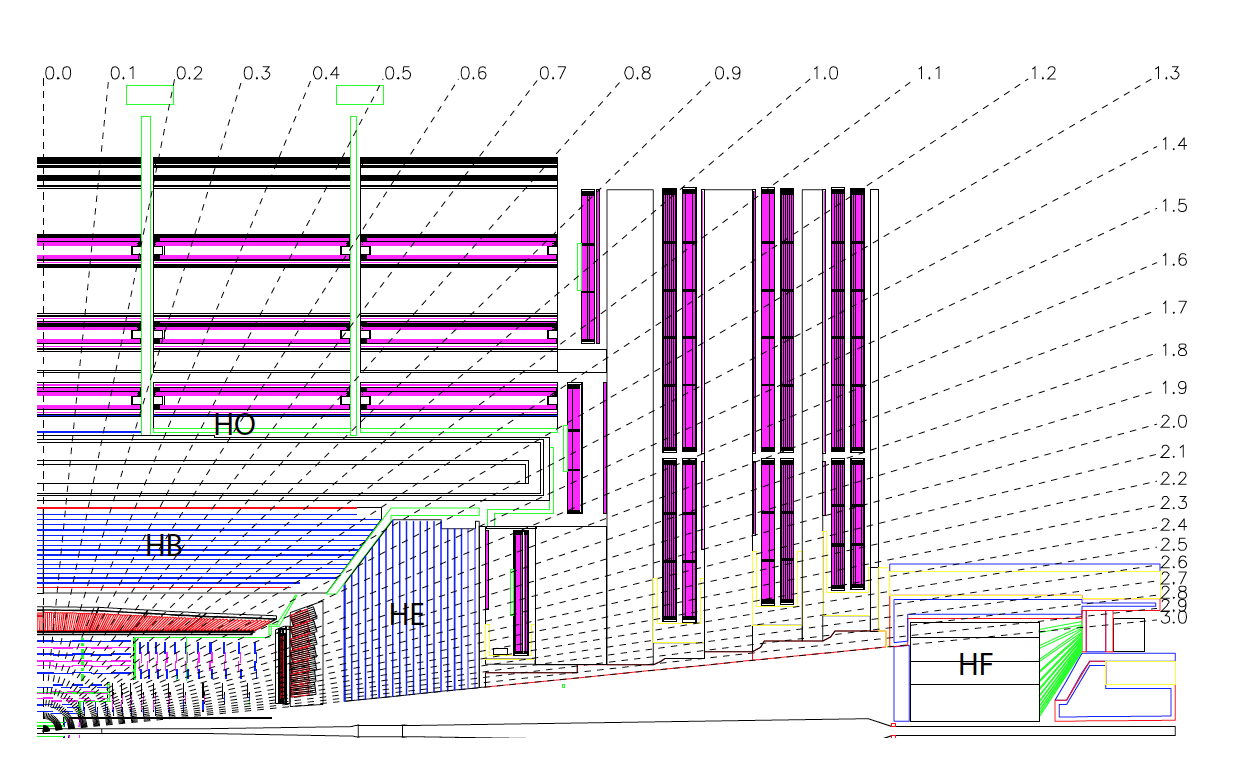
\includegraphics[scale=0.65]{figures/hcal}
	\caption{A projection of the HCAL, highlighting its subdetectors~\cite{Chatrchyan:2008aa}.}
	\label{hcal}
\end{figure}

The HB comprises 36 identical wedges forming two cylindrical half-barrels, each 4.3~m long. This subdetector extends radially between $1.77 < r < 2.95$~m and is located between the EB and solenoid, covering the region $|\eta| < 1.3$. Although the HB provides excellent shower containment in this region, the HO is added outside of the solenoid, which it uses as an absorber, to provide additional detection for shower tails that may extend outside of the HB. The combination of the HB and HO provide an effective thickness of a minimum of 11.8 nuclear interaction lengths ($\lambda_\mathrm{I}$). Each HE is located between $3.9 < |z| < 5.7$~m  and covers the range $1.3 < |\eta| < 3.0$. The granularity provided by the HB and HEs is $\Delta\eta{\times}\Delta\phi = 0.087{\times}0.087$ for $|\eta| < 1.6$ and $\Delta\eta{\times}\Delta\phi = 0.174{\times}0.174$ for $|\eta| \ge 1.6$. The scintillation light from the tiles across the depth of a single $\Delta\eta{\times}\Delta\phi$ region in the HB or an HE is optically added, forming a tower.

The coverage provided by the HEs is extended by the HFs to $|\eta| = 5.2$. Each HF is located at $z = 11.2$~m and uses quartz fibers embedded in a steel absorber to deal with some of the highest particle fluxes in the detector, minimizing radiation damage. Particle showers in the fibers emit Cherenkov radiation, which is detected by photomultiplier tubes. Each HF uses both long and short fibers interlaced throughout its detector volume. Both fibers run the full HF depth of 165~cm (10~$\lambda_\mathrm{I}$), but the short fibers start 22~cm from the front end. Both fibers are read out separately to allow for the discrimination between electromagnetic and hadron showers. The former deposit most of their energy within the first 22~cm, while the latter produce nearly equal signals in both calorimeter segments.


\subsection{Muon System}

The muon system is designed to provide robust muon identification with precise measurements of muon momenta. This subdetector is arranged in a muon barrel (MB) and muon endcap (ME) configuration, consisting of three types of gas ionization chambers: drift tube chambers (DTs), cathode strip chambers (CSCs), and resistive plate chambers (RPCs). The DTs are segmented into drift cells that measure the positions of muons by determining a drift time through an electric field to an anode wire of a cell. The CSCs are multi-wire proportional counters using a highly segmented cathode strip readout capable of providing an accurate measurement of the positions of the muons in the $r$-$\phi$ magnetic bending plane. The RPCs are double-gap chambers that operate in avalanche mode with a fast response and primarily provide timing information for the muon trigger. These chambers are embedded in the steel flux-return yoke outside of the solenoid. Fig.~\ref{fig:muon_system} shows a schematic highlighting these different features of the muon system.

\begin{figure}[!htb]
	\centering
	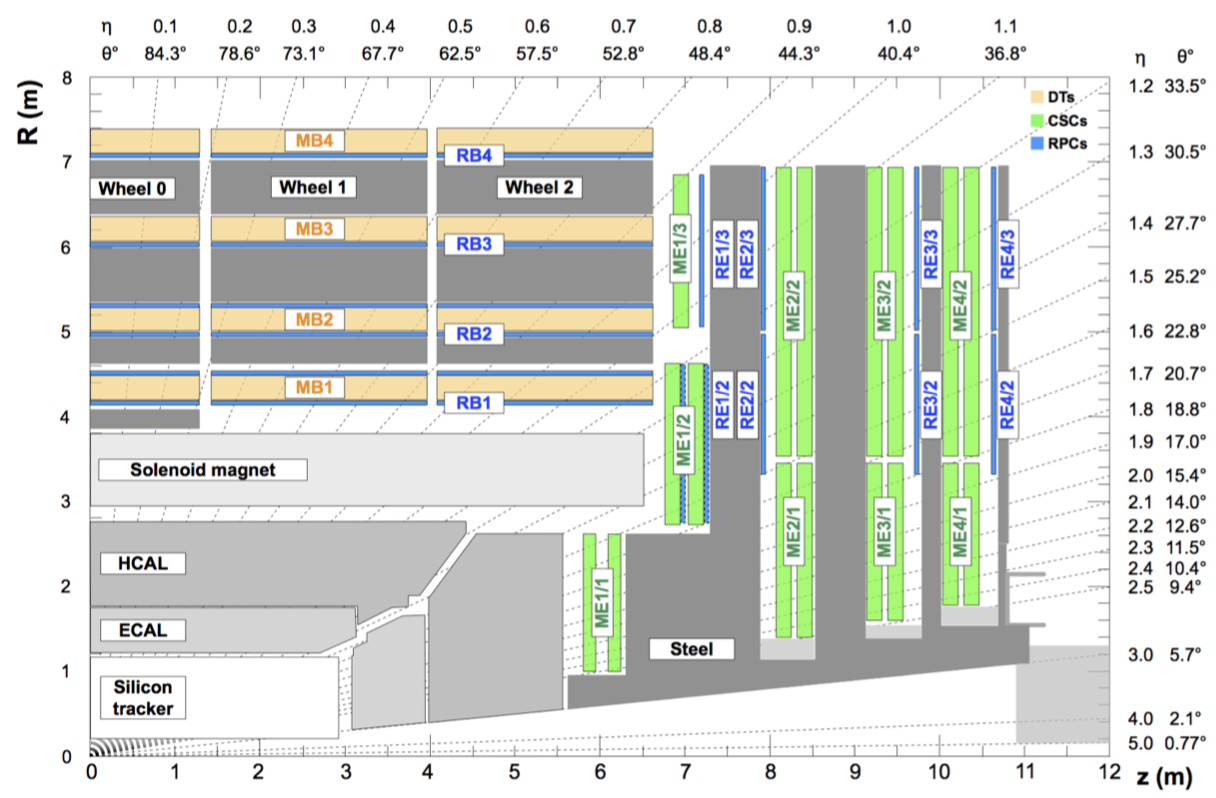
\includegraphics[width=0.85\textwidth]{figures/muon_chambers.png}
	\caption{A schematic of the CMS muon system depicting its major components and their detector coverage~\cite{Sirunyan:2018fpa}.}
	\label{fig:muon_system}
\end{figure}

The MB covers the region with $|\eta| < 1.2$ using DTs, chosen for the suitable detector conditions in that region: a uniform magnetic field, low neutron induced background, and small muon rates. The DTs are arranged into 4 stations, containing 8 chambers capable of measuring the muon position in the $r$-$\phi$ plane. The first 3 stations have 4 additional chambers allowing for position measurements along the $z$-axis. The MEs cover the region between $0.9 < |\eta| < 2.4$ using CSCs, which can handle the non-uniform magnetic field, high background levels, and large muon rates. Each ME has 4 stations of CSCs comprised of chambers positioned perpendicular to the beam line, providing the full position measurements and beam crossing times for the muons. To complement the DTs and CSCs, the RPCs are added to both the MB and MEs, covering $|\eta| < 1.6$. Their fast response provides good time resolution, but, compared to the DTs and CSCs, a coarser position resolution. There are 6 layers of RPCs embedded in the MB and 3 layers in each ME. Altogether, this provides a muon system capable of triggering on muon \pt with high efficiency ($>$90\% over the entire $\eta$ range) and excellent background rejection, while providing a muon \pt resolution of less than 7\% in the MB for muon $\pt < 1\TeV$ and a muon timing resolution of approximately 1.4~ns~\cite{Sirunyan:2018fpa}. The performance of the muon system is presented in Ref.~\cite{Sirunyan:2018fpa}, and further discussion on muon reconstruction is given in Section~\ref{sec:event_reco}.


\subsection{Trigger System}

The LHC provides proton-proton collisions at high rates, occurring every 25~ns, corresponding to a frequency of 40~MHz. This challenging environment is further complicated by the presence of pileup, which is multiple pp interactions occurring within the same event from a single proton-proton bunch crossing. This type of pileup is in-time with the bunch crossing, but pileup can also occur out-of-time from bunch crossings just before and after the collision of interest. When a subdetector's electronics are integrated for more than 25~ns, its response becomes sensitive to out-of-time pileup. The amount of pileup recorded by the CMS detector during each of its data taking years is plotted in Fig.~\ref{fig:CMS_pileup}. \correction{An average of 37 simultaneous pp interactions occurred during the 2018 LHC data taking period} using $\sqrt{s} = 13\TeV$. At these high rates with this large amount of pileup, it is not feasible to fully process, reconstruct, and store all of the data for each event, so a significant reduction needs to be made. This is accomplished by the trigger system, which functions in two stages: the Level-1 (L1) trigger and high-level trigger (HLT) stages.

\begin{figure}[!htb]
	\centering
	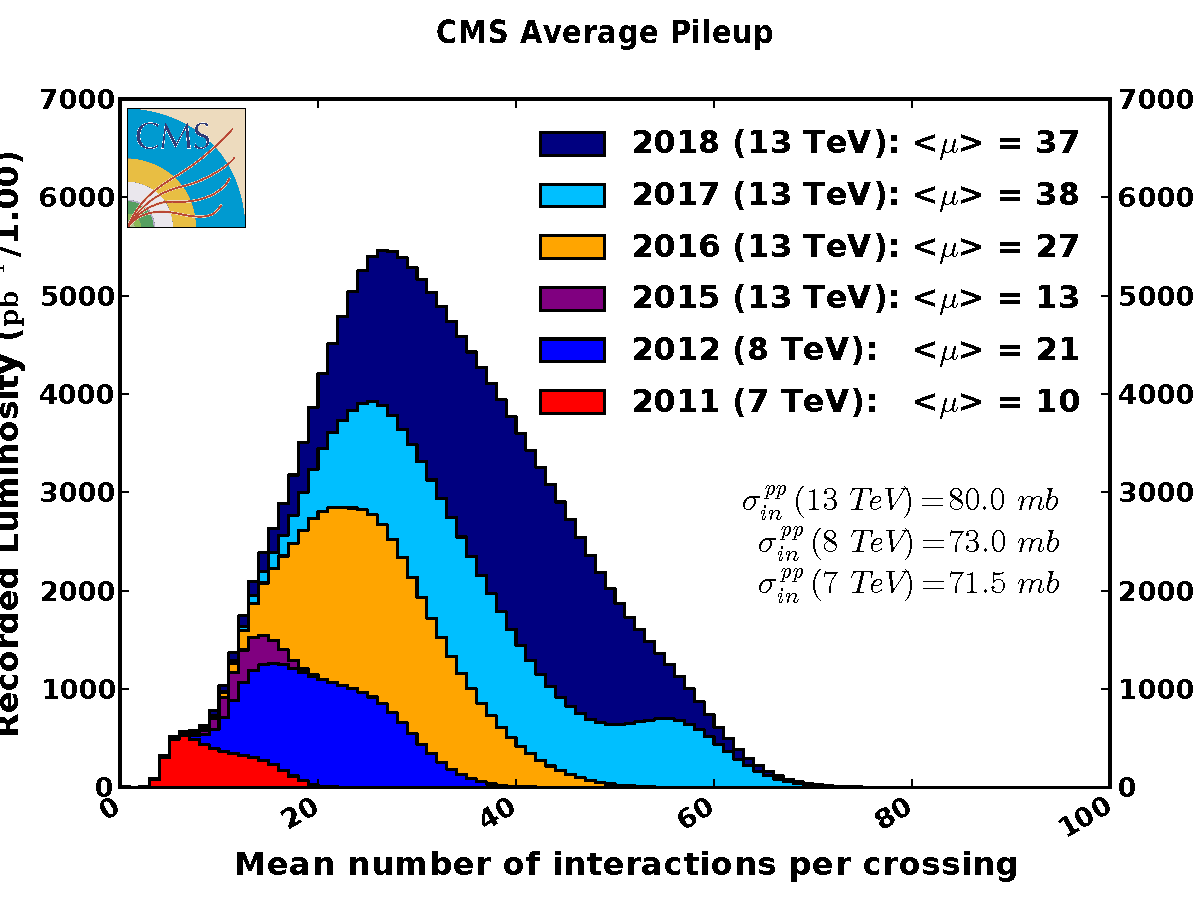
\includegraphics[width=0.63\textwidth]{figures/pileup_allYears_stack.pdf}
	\caption{The average amount of pileup recorded by the CMS detector during each of its data taking years~\cite{CMS_lumi}. The histograms from each year are stacked on the previous year. Also printed are the measured pp interaction cross sections for the different center-of-mass energies used during each data taking period.}
	\label{fig:CMS_pileup}
\end{figure}

The L1 trigger is made up of custom designed and programmable hardware. It analyzes every bunch crossing and is capable of selecting events in order to determine whether or not they should be further processed. This is achieved at a rate of around 100~kHz, with a latency of 3.2~$\mu$s. The L1 trigger uses information from the ECAL, HCAL, and muon system. The inner tracking system takes too long for readout at this stage and is only read out after the event of interest passes the L1 trigger. The calorimeters provide the L1 trigger with trigger primitives based on the presence of large energy deposits. This information is passed to regional and global components of the trigger, where event-level quantities are determined, such as jets, photon/electron candidates, traverse energy, and missing transverse energy. The muon system works to provide track information and muon candidates. The L1 trigger takes the final information provided by these subsystems and generates an L1 Accept (L1A) if trigger criteria are met, marking the event to be fully read out. Upon generation of an L1A, the detector information is passed to the HLT, which reconstructs the event and decides whether or not it should be saved. These steps are described in the flowchart in Fig.~\ref{fig:L1_trigger}. A more detailed description can be found in Ref.~\cite{Khachatryan:2016bia}.

\begin{figure}[!htb]
	\centering
	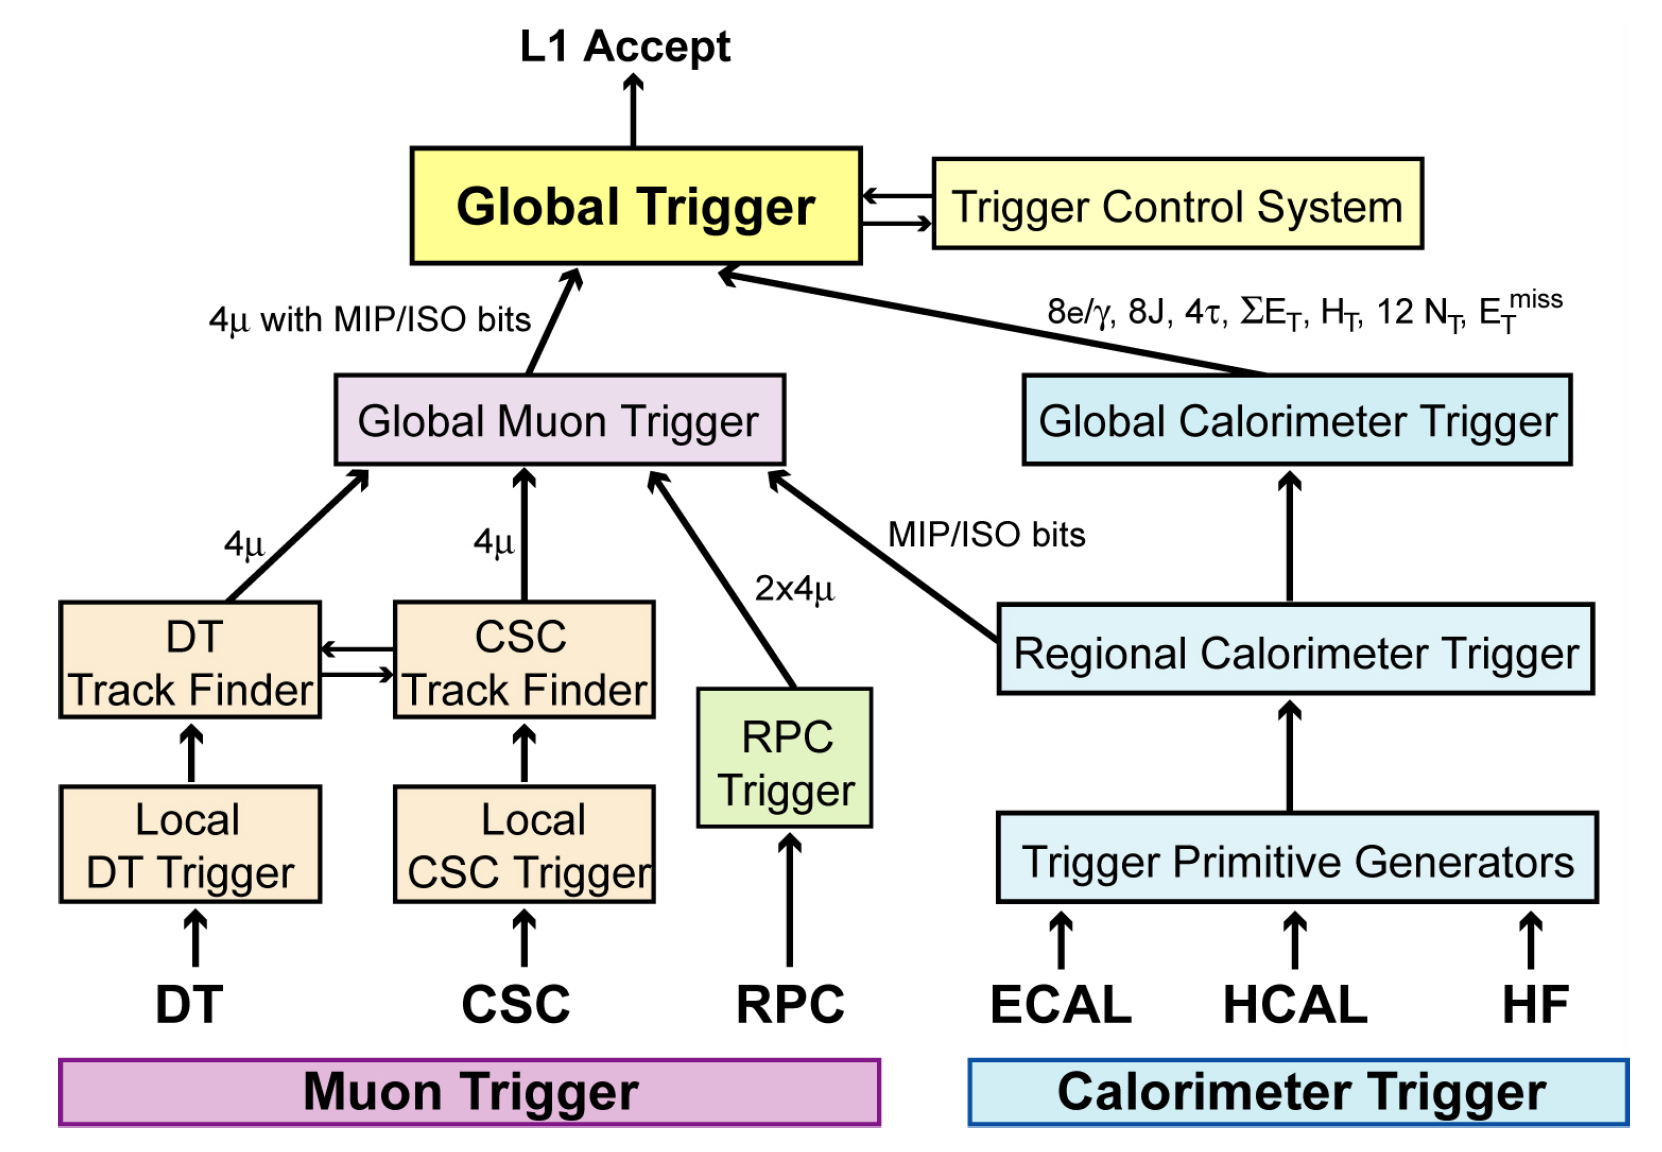
\includegraphics[width=0.70\textwidth]{figures/L1_trigger.png}
	\caption{A flowchart showing how the global, regional, and local components of the L1 trigger system operate to produce an L1A~\cite{Chatrchyan:2008aa}.}
	\label{fig:L1_trigger}
\end{figure}


The HLT consists of a processor farm running the full CMS online event reconstruction software, which can be continuously updated to meet experimental needs. A sophisticated data acquisition (DAQ) system works with the trigger system to collect and analyze the event information from each LHC bunch crossing. At designed luminosity, the LHC delivers about 1~MB/event of zero-suppressed data containing the full CMS detector information. The DAQ is designed to sustain a maximum input rate of 100~kHz and a data flow rate of approximately 100~GB/s. The HLT reduces the event rate to about 1~kHz. Events are uniquely specified by their run number, luminosity section of the LHC fill, and event number, all specific to the CMS DAQ system.





\chapter{Event Reconstruction and Selection}\label{ch:event_selection}

Events are recorded and reconstructed in the CMS detector, then further selection criteria are imposed in order to determine analysis-level physics objects. General event reconstruction will be discussed, followed by the specific diphoton event selection used in this analysis.


\section{Event Reconstruction}\label{sec:event_reco}

After events are recorded by the CMS detector, they are reconstructed through a variety of algorithms into their constituent components. All electrically charged particles produce signals in the pixel and strip tracking system. Muons are detected within the muon system before, generally, leaving the detector. Electrons and photons deposit most of their energies in the ECAL, while charged and neutral hadrons mostly deposit in the HCAL. The electrical signals produced by each subdetector are read out and converted into physics object candidates. Each subdetector can individually generate different particle candidates; however, CMS uses particle-flow (PF) global event reconstruction~\cite{CMS-PRF-14-001} to identify and reconstruct individual particles (namely, electrons, muons, photons, charged hadrons, and neutral hadrons) using information from all subdetectors. Jets, missing transverse energy, and other composite objects are built using the PF algorithm.

\subsection{Tracks and Vertices}\label{sec:track_vertex}

The trajectories of charged particles form tracks as they propagate as helices between the tracker layers. Tracks are fundamental for event reconstruction, contributing towards the subsequent reconstruction of other physics objects in the event. CMS uses the Combinatorial Track Finder (CTF) algorithm, which is based on a Kalman filter, for track reconstruction, as described in Ref.~\cite{Chatrchyan:2014fea}. The CTF fits tracker hits, while taking into account the uncertainty of the hit positions and the effects of multiple Coulomb scattering and energy loss. The fit returns track information, including charge, initial momentum, and its impact parameter with respect to the primary vertex.

Primary vertices are those compatible with the hard scattering from the pp interactions along the beam line. Secondary vertices in the event can result from particle decays after the hard interaction. The primary vertex is reconstructed by selecting and clustering tracks compatible with the LHC beam spot, which is the 3D luminous region where the LHC beams collide. The track clustering is done using a deterministic annealing algorithm, and the position of each vertex is fit for using its associated tracks, as described in Ref.~\cite{Chatrchyan:2014fea}. Due to pileup, multiple primary vertices can be reconstructed in an event. However, the main primary vertex is chosen to be the reconstructed vertex with the largest value of summed charged-particle track $\pt^2$, with additional constraints described in Section~9.4.1 of Ref.~\cite{Contardo:2020886}. This selected vertex is simply referred to as the primary vertex. The position resolution for primary vertices is between 10-12~$\mu$m for each of its three spatial coordinates~\cite{Chatrchyan:2014fea}.


\subsection{Photons and Electrons}

Photon candidates are reconstructed from energy deposits in the ECAL. Before entering the ECAL, a photon may convert in the tracker into an electron-positron pair, whose paths bend under the influence of the magnetic field, causing their energy deposits to be extended along the $\phi$ direction. Individual energy deposits are grouped into superclusters to allow maximal recovery, using different procedures in the EB and EE regions. ECAL crystals are aligned in an $(\eta, \phi)$ grid in the EB and an $(x, y)$ grid in either EE. First, clusters are built starting with a seed crystal, which is located by selecting the crystal with the highest $E_{\mathrm{T}}$ above a certain threshold among its neighboring crystals. Next, in the EB region, a $5{\times}1$ bar of crystals centered on a seed is formed along the $\eta$ direction. Connected bars within $\pm17$ crystals along $\phi$ from the seed crystal are added if their total energy is above some threshold, forming a cluster. Other clusters, built in this way, having seeds aligned in $\eta$ with this cluster's seed are added, based on a further threshold requirement, to form superclusters. In the EE regions, a cluster of a $5{\times}5$ array of crystals centered on a seed is first built. The crystals surrounding the $5{\times}5$ boundary are allowed to seed new $5{\times}5$ clusters using crystals not included in any cluster yet. The clusters are allowed to partially overlap, and a supercluster is formed from the connected clusters. In either the EB or an EE, the superclusters formed for unconverted photons are typically $5{\times}5$ matrices. Further details are described in Ref.~\cite{CMS:EGM-14-001}.

The raw energy for photons is obtained by summing the energy deposits in the supercluster, corrected for detector effects, as described in Section~\ref{sec:ECAL}. Energy deposited in an ECAL preshower detector is added to the photon energy measurement from the adjacent EE. This \correction{raw energy needs to be corrected,} mainly to account for photon shower loss and contamination from pileup. The shower may be lost between gaps in the crystals or through gaps in the ECAL modules, resulting in parts of the shower not being clustered into the supercluster. Data-driven scale factors for the photon energy scale and resolution are extracted from $Z \to e^+e^-$ decays, with electrons reconstructed as photons, using an energy regression based on a boosted decision tree (BDT)~\cite{CMS:EGM-14-001}. Because of the limited dynamic range of the ECAL readout electronics, they saturate when the energy deposited in a single crystal is greater than an average value of about 1.7 (2.8)\TeV in the EB (EEs), with a spread of about 10 (25)\% among different channels. Energy corrections to account for this are derived using a simulated sample of photon candidates with energies spanning a large range. The photon energy scale and resolution are corrected by comparing the difference between data and simulation from $Z \to e^+e^-$ events, calibrated at the $Z$ boson peak. The difference in energy scale is used to correct the data. The energy resolution in simulation needs additional Gaussian smearing to match that of data, which is considered as a correction. In the EB, photons in the range of tens of {\GeVns} have an energy resolution of about 1\%, while photons above this range have a resolution of about 1.3\% up to $|\eta| = 1$, rising to about 2.5\% at $|\eta| = 1.4$. In each EE, the energy resolution for photons in the range of tens of {\GeVns} is about 2.5\%, while photons above this range have a resolution between 3 and 4\%~\cite{CMS:EGM-14-001}.

Electrons are reconstructed by matching a track to an ECAL supercluster, determined using the same method as for photons. The electron track reconstruction uses a Gaussian sum filter (GSF) to fit the tracker hits. The emitted bremsstrahlung photons, which can carry away a significant fraction of the initial electron energy, can convert into electron-positron pairs, yielding secondary tracks. This is taken into account by the GSF. The details are described in Ref.~\cite{Khachatryan:2015hwa}.


\subsection{Muons and Tau Leptons}

Muon reconstruction uses information from both the muon system and inner tracker. Muon tracks are first reconstructed in the muon system to form track segments generated by requiring a certain number of hits in the layers within a single DT or CSC chamber. These segments are then fit, with information from the RPCs included, to form standalone muons. These standalone candidates are then matched to tracks from the inner tracking system by projecting the standalone muon trajectories to the outer tracker surface and using a method similar to the CTF algorithm (see Ref.~\cite{Sirunyan:2018fpa} for details). Muon performance was discussed in Chapter~\ref{ch:experiment}.

The $\tau$ lepton signature is more complex than for electrons or muons. They are the heaviest of the charged leptons, with a short lifetime, and will typically decay before reaching the active material of the detector. About 2/3 of the time, $\tau$ leptons decay hadronically and can be reconstructed indirectly through their PF candidate decay products. The performance of $\tau$ lepton reconstruction and identification is presented in Refs.~\cite{Chatrchyan:2012zz,Sirunyan:2018pgf}.

\subsection{Jets and Missing Transverse Energy}\label{sec:jets}

A typical proton-proton collision will produce quarks or gluons either through the hard interaction directly or through QCD radiation from the initial or final state partons. Due to QCD confinement, colored partons are not freely observed. Instead, they transform into a collection of color-neutral hadrons, observed as a cluster of particles called jets. Because the number of color states for gluons is larger than for quarks, gluon-initiated jets, in general, have higher particle multiplicity, a softer fragmentation function, and are less collimated than quark-initiated jets~\cite{CMS:2013kfa,Aad:2014gea}. So, quark jets tend to have lower multiplicity, harder constituents, and are narrower. In addition, quarks have electrical charge, while gluons do not. Jets can be further classified according to their quark flavor. Heavy-flavor jets originate from $b$ or $c$ quarks, while light-flavor jets are those originating from $u$, $d$, or $s$ quarks. In some cases, jet identification techniques are able to discriminate between these different types of jets~\cite{Asquith:2018igt,Sirunyan:2017ezt}. Top quarks decay before they hadronize and are identified through their decay products (see, e.g., Ref.~\cite{Sirunyan:2017huu}).

Jets are built from PF candidates, primarily detected as charged hadrons (e.g., $\pi^{\pm}$, $K^{\pm}$, and protons), neutral hadrons (e.g, $K^0_{\mathrm{L}}$ and neutrons), or nonisolated photons (e.g., from $\pi^0$ decays). The energy deposits are calibrated to account for the nonlinear response of the calorimeters, and reconstructed tracks are compared to the clusters. The energy deposits are clustered into jets using the infrared and collinear safe anti-$k_{\mathrm{T}}$ algorithm~\cite{Cacciari:2008gp,Cacciari:2011ma}, with a distance parameter of $R = 0.4$. Infrared (collinear) safety means the jet algorithm remains invariant under soft emission (co-moving / collinear momentum splitting) of the clustered particles. Heavy-flavor jets will typically produce a secondary vertex. For example, a $B$ meson such as a $B^{+}$ will travel an average distance of approximately 500~$\mu$m before decaying. This is well within the vertex resolution of the tracking system. Jets originating from $b$ quarks are identified with the combined secondary vertex (CSVv2) $b$ tagging algorithm~\cite{Sirunyan:2017ezt}. Since the lifetime of a $c$ quark is shorter than that of a $b$ quark, a similar, but modified, procedure is used for $c$ jet identification, discussed in Ref.~\cite{Sirunyan:2017ezt}.

Neutrinos interact only through the weak interaction and escape through the detector. This is also true for any (stable) electrically neutral, colorless particle. Nonetheless, their presence can be inferred through a momentum imbalance in the collision using conservation of momentum, given that the initial transverse momentum of the colliding system is negligible. In the transverse plane, this would show up as missing $E_\mathrm{T}$, referred to as MET, equal to $\left| -\sum{\vec{\pt}}\right|$. Along the longitudinal axis, the missing $E_\mathrm{z}$ is not useful since the initial longitudinal momenta of the colliding partons within the protons are unknown.


\section{Event Selection}

The signature in this analysis consists of two high-energy, prompt photons. Events containing this signature are reconstructed and required to pass a trigger selection. These photons form diphoton candidates, which are required to pass a preselection and further identification criteria, imposed to obtain high event purity with high search sensitivity.

\subsection{Trigger Selection}\label{sec:trigger}

Events are selected which pass the CMS HLT trigger with path name \texttt{HLT\_DoublePhoton60}. These events contain at least two photon candidates, each with $\pt>60\GeV$, across the range $|\eta| < 3.0$. The primary selection at this level requires each photon candidate to have $\hoe < 0.15$. The longitudinal shower shape variable $\hoe$ is defined as the ratio of the hadronic to electromagnetic energy fraction of the photon candidate. The electromagnetic energy fraction is defined as the corrected supercluster energy. At this trigger level, the hadronic energy fraction is defined as the total HCAL energy within a cone of $\Delta R < 0.15$ from the supercluster position, as used in the variable referred to as $\text{Hadronic/E}$ in Section~\ref{sec:fake_background}. Later, at the analysis level, this fraction will mean the amount of HCAL energy in the tower directly behind the photon seed crystal. This trigger is seeded by the logical OR of a suite of \texttt{SingleEG}, \texttt{DoubleEG}, \texttt{SingleJet}, and \texttt{SingleTau} CMS L1 seeds, with varying thresholds. These thresholds are primarily sensitive to one or two large electromagnetic energy deposits, a large hadronic energy deposit, or a signature in the muon and calorimeter systems consistent with the presence of a single $\tau$ lepton decay, respectively.

The trigger efficiency measured relative to the \texttt{HLT\_DoublePhoton40} trigger, which requires the two photon candidates to each have $\pt>40\GeV$, is shown in Fig.~\ref{fig:relative_trigger_efficiency}. The photons are ordered by \pt in each event, with the leading photon having the highest \pt and the subleading photon having the second highest. The efficiency shown here is measured as a function of the subleading photon \pt. This selection is fully efficient above photon $\pt > 75\GeV$.

\begin{figure}[!htbp]
	\centering
	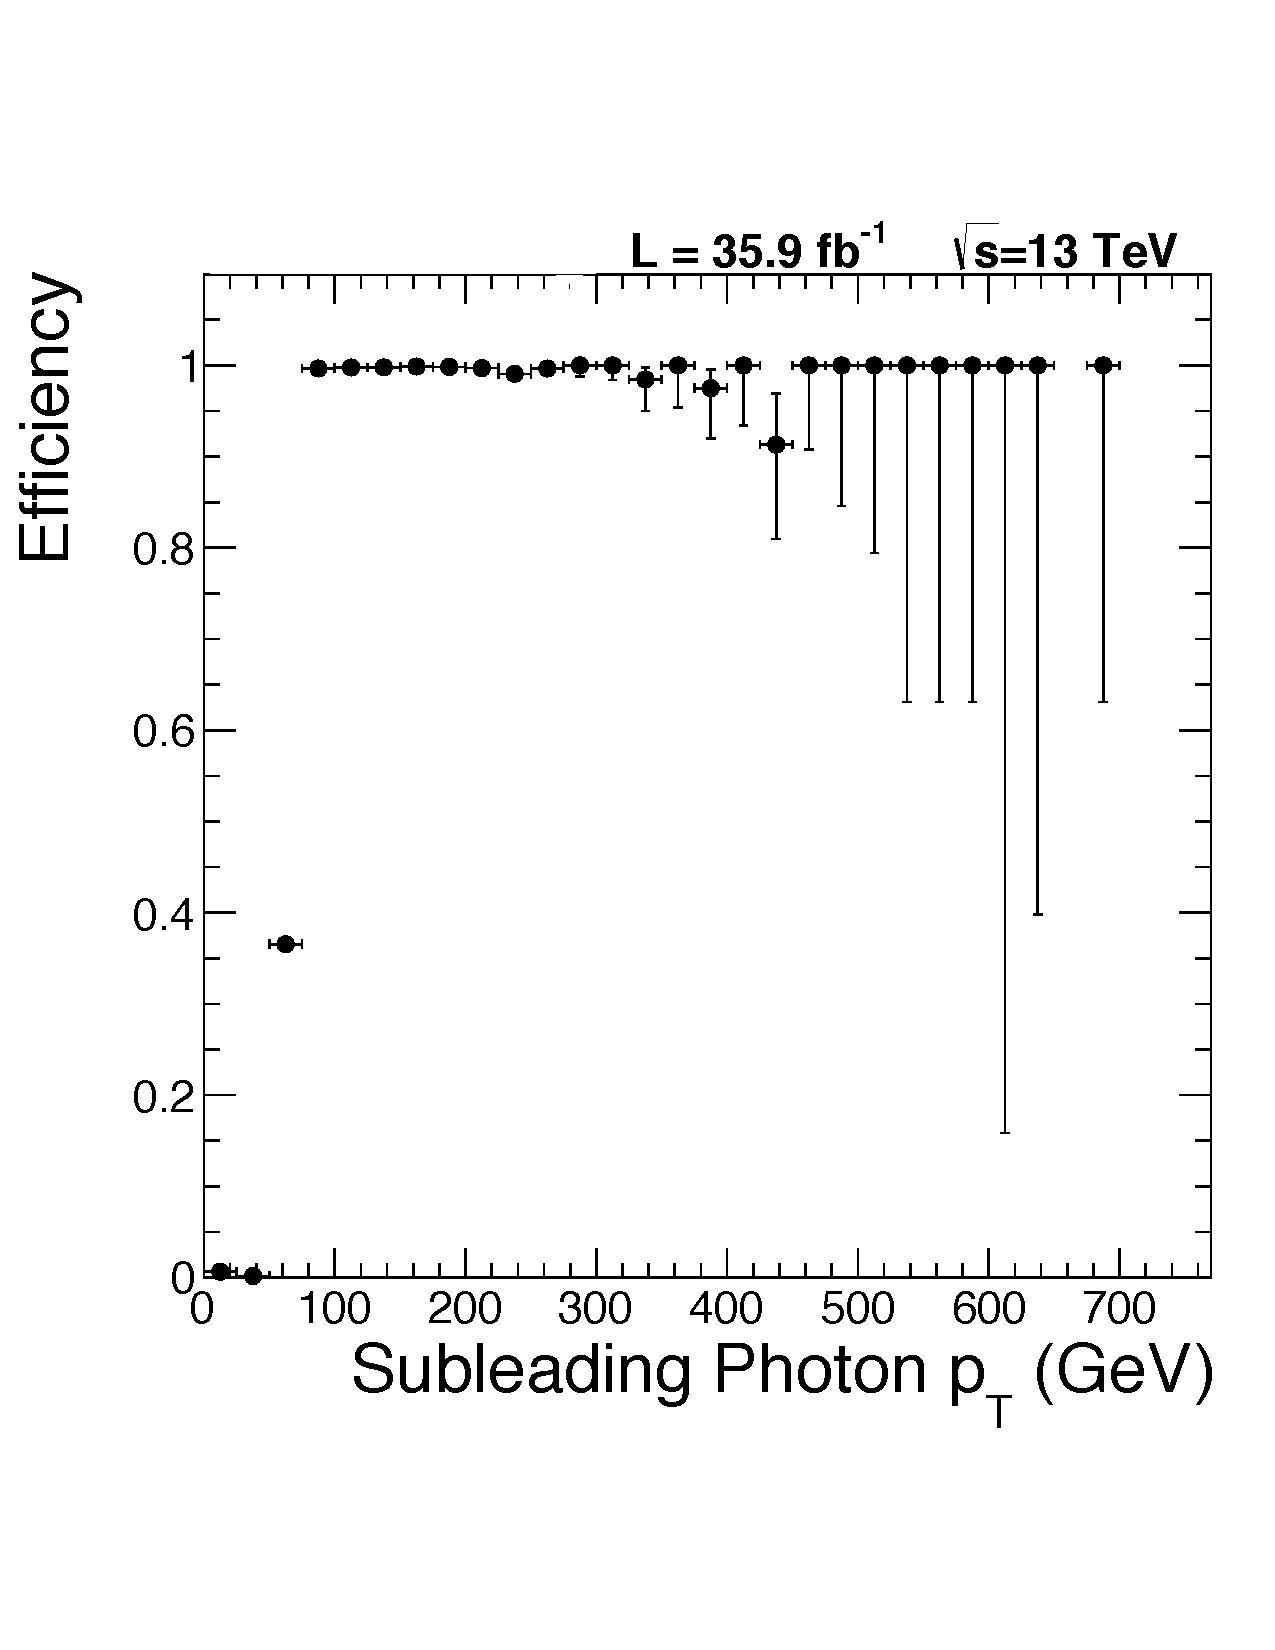
\includegraphics[angle=0,width=0.55\textwidth]{figures/eff2016.pdf}
	\caption{The relative efficiency of the \texttt{HLT\_DoublePhoton60} trigger (measured with reference to the \texttt{HLT\_DoublePhoton40} trigger) as a function of the \pt of the subleading photon.}
	\label{fig:relative_trigger_efficiency}
\end{figure}

The absolute trigger efficiency of \texttt{HLT\_DoublePhoton60} was measured using a simulated sample of diphoton events, similar to those described in Chapter~\ref{ch:signal}. In this simulated sample, the diphoton invariant mass \mgg is known and can be compared before and after imposing the trigger selection. Fig.~\ref{fig:absolute_trigger_efficiency} shows the trigger efficiency as a function of \mgg, which is fully efficient for events with $\mgg > 500\GeV$. The two plots shown correspond to the different analysis event categories, which will be explained in the following section.

\begin{figure}[!htbp]
	\centering
  	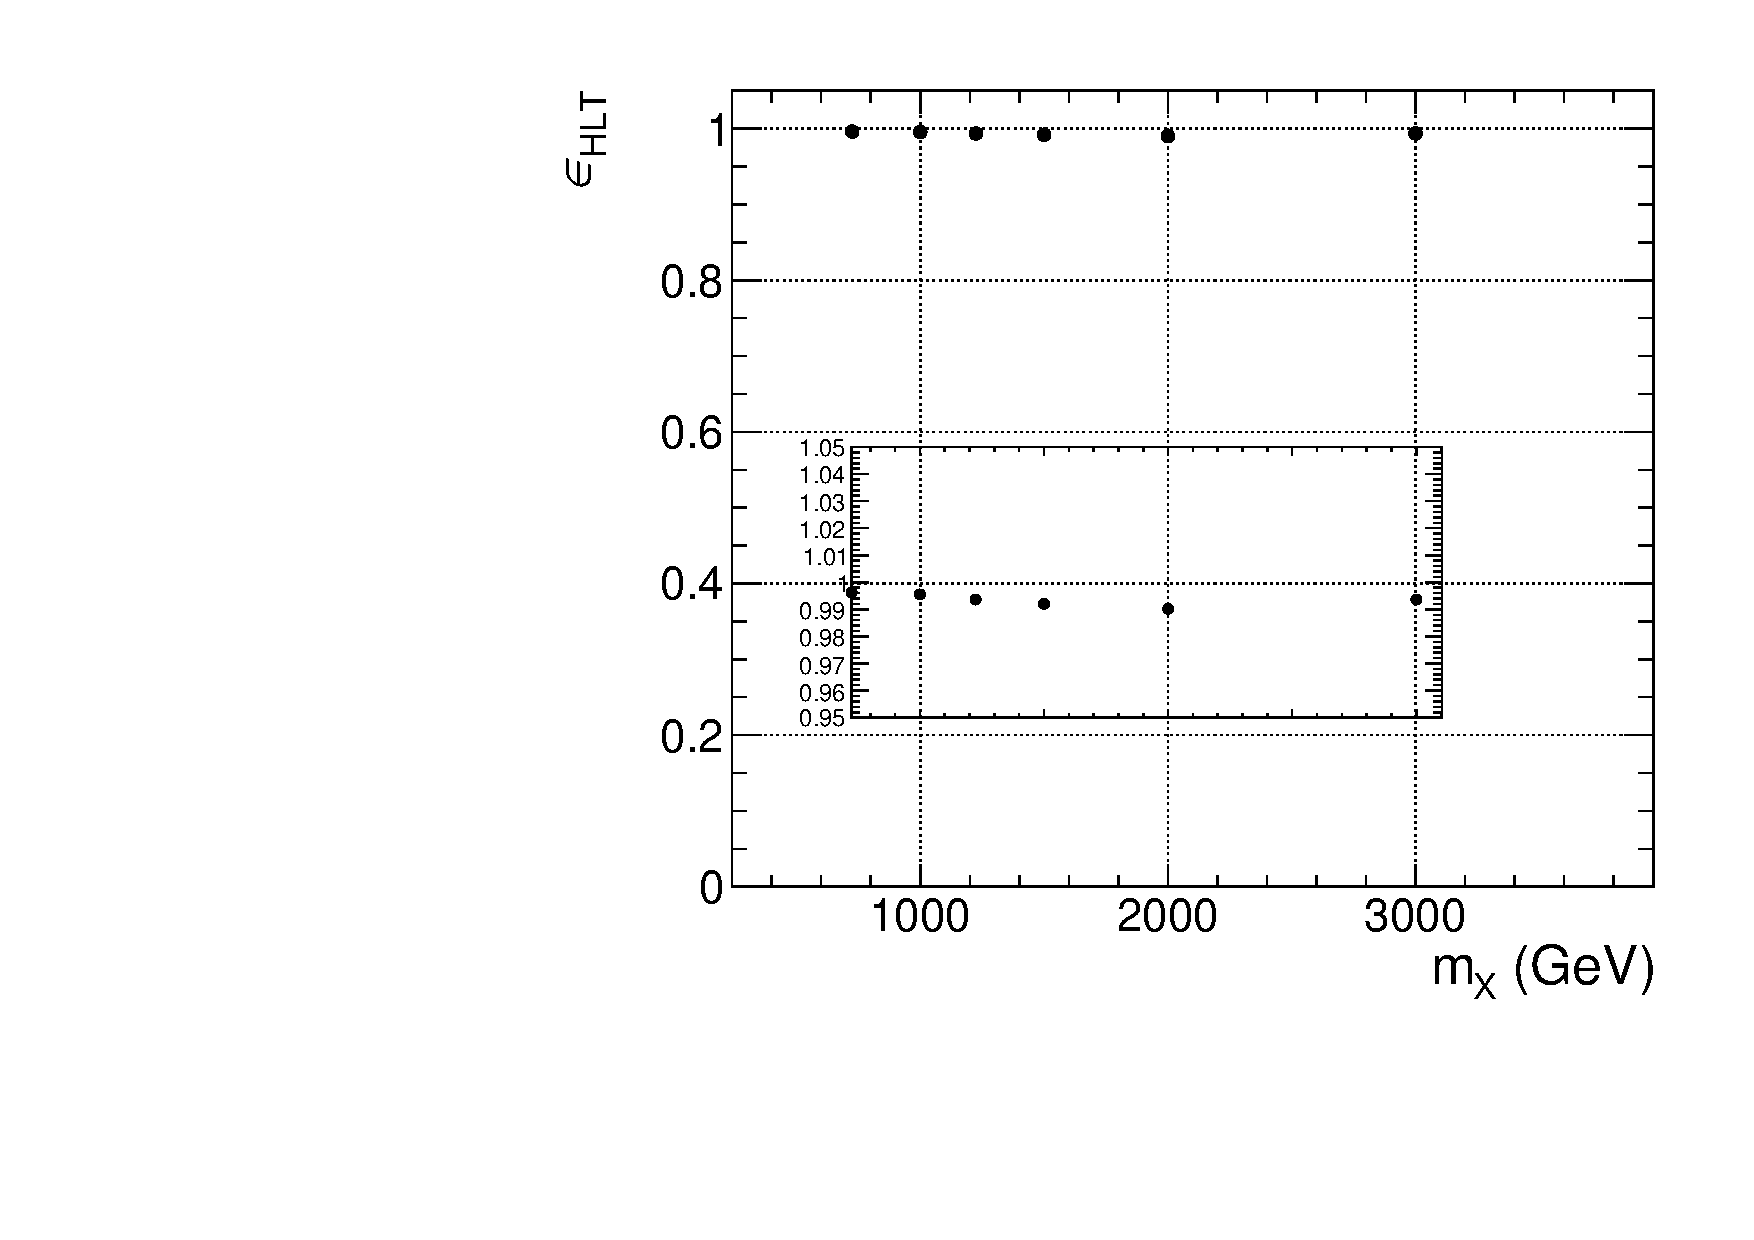
\includegraphics[angle=0,width=0.49\textwidth]{figures/eff_dipho60_EBEB_vs_mass}
	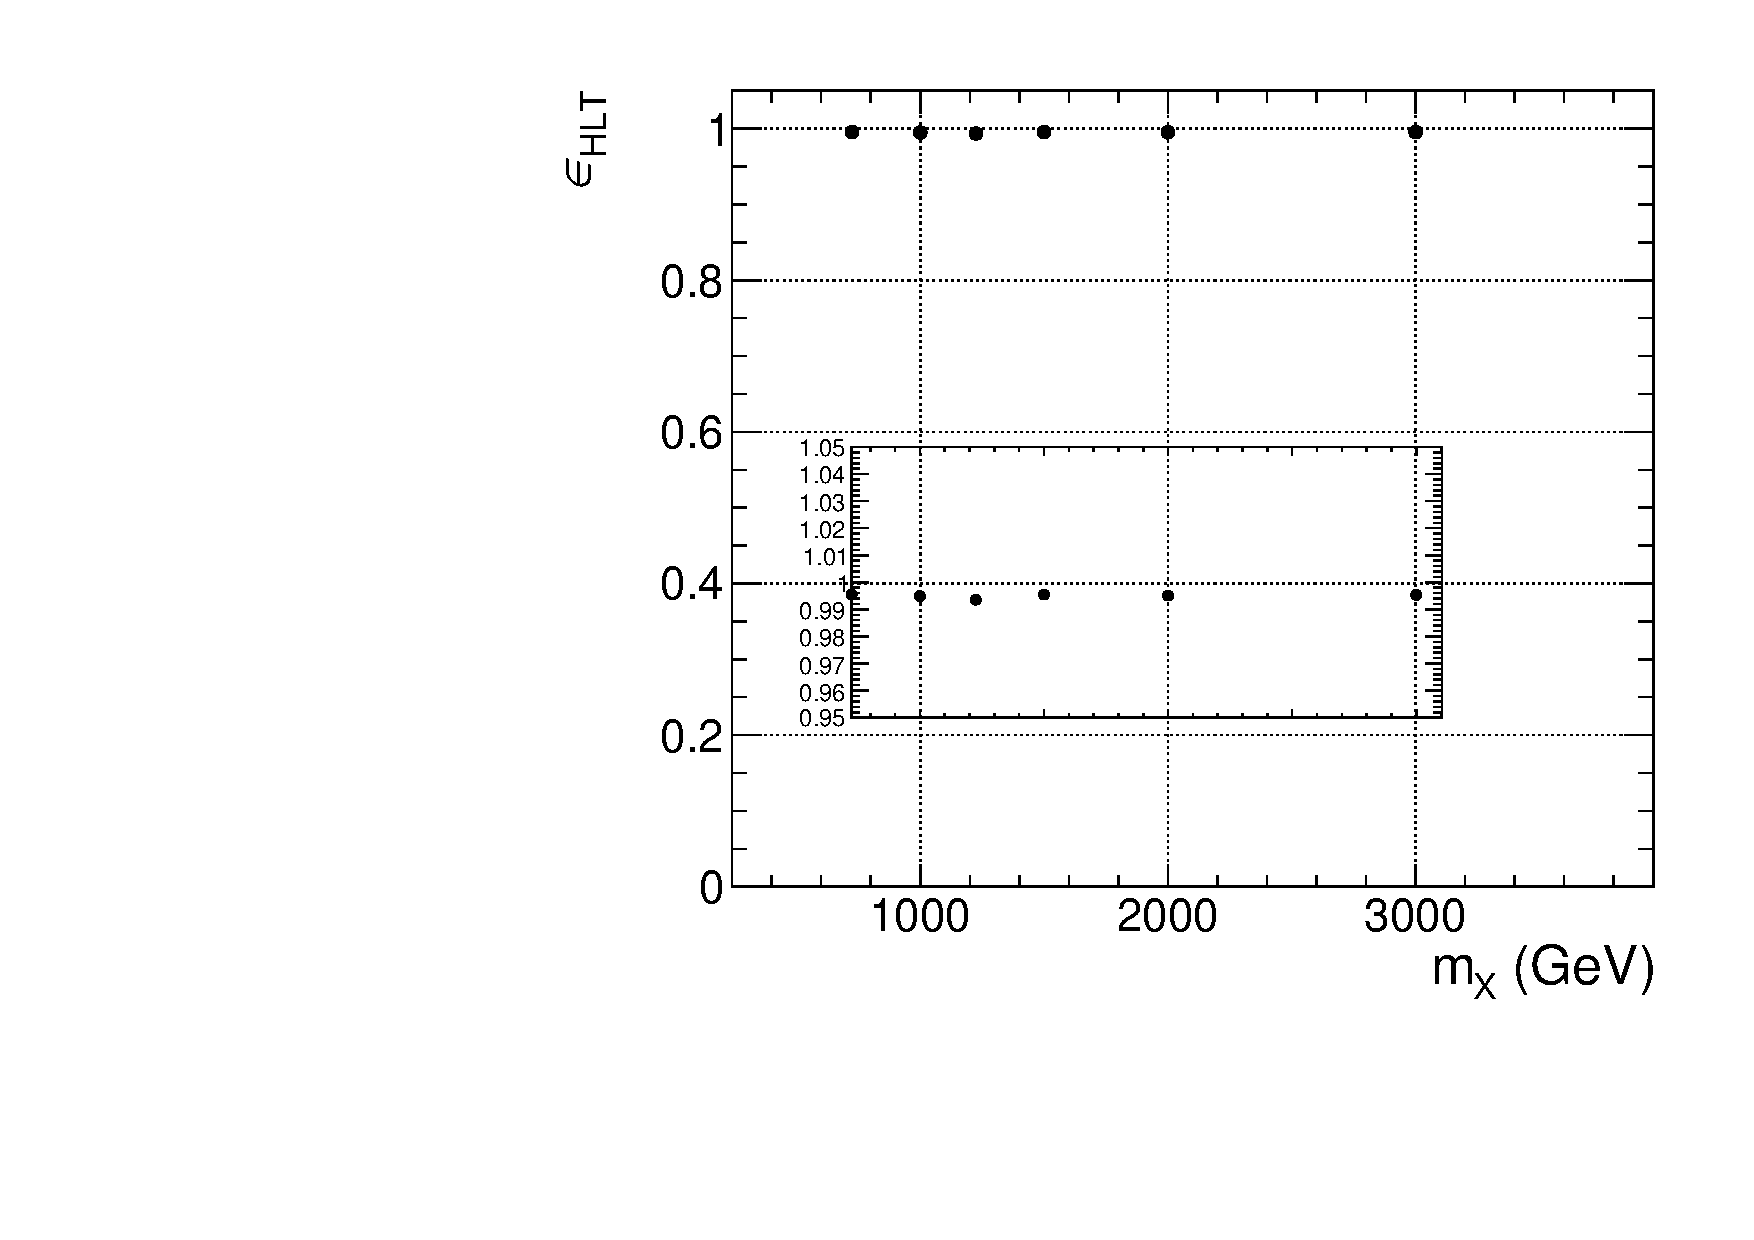
\includegraphics[angle=0,width=0.49\textwidth]{figures/eff_dipho60_EBEE_vs_mass}
	\caption{The absolute efficiency of the \texttt{HLT\_DoublePhoton60} trigger (measured using a simulated diphoton sample) as a function of $m_\mathrm{X} =\mgg$ in the EBEB (left) and EBEE (right) categories. The inner boxes show a zoomed-in region of the $y$-axis.}
	\label{fig:absolute_trigger_efficiency}
\end{figure}

To protect against potentially missing high-mass diphoton candidates at the trigger level, the backup trigger \texttt{HLT\_ECALHT800} is applied in addition to \texttt{HLT\_DoublePhoton60}. This triggers solely on the presence of large energy deposits in the ECAL without imposing additional criteria, such as a selection in \texttt{HLT\_DoublePhoton60} that could be responsible for causing the diphoton candidates to be rejected. The contribution from \texttt{HLT\_ECALHT800} to the analysis dataset is minimal (yielding $\sim$10 events).


\subsection{Event Preselection}

After trigger selection, candidate diphoton events are required to satisfy the following kinematic selection:
\begin{itemize}
	\item{each photon candidate is required to have $\pt>75\GeV$;}
	\item{one photon is required to be in the EB with $|\eta| < 1.4442$, and another in either the EB or in an EE, where it must have $1.566 < |\eta| < 2.5$;}
	\item{the photon pair must satisfy $\Delta R > 0.45$; and}
	\item{$\mgg>500\GeV$.}
\end{itemize}
\correction{The trigger efficiency measurements are one of the motivations for the photon $\pt>75\GeV$ and $\mgg>500\GeV$ requirements.} In this analysis, there are two signal regions considered: one with both photons in the EB, denoted EBEB, and the other with one photon in the EB and the other in either EE, denoted EBEE. Events with both photon candidates in the EEs are dominated by SM production and have negligible sensitivity to the target BSM signal, and thus are omitted from this analysis. Additional categories were considered, but were also excluded for this reason. We use the fiducial region of the ECAL, defined with a restricted $\eta$ range, as specified above, which rejects events outside of the tracker coverage and in the gap between the EB and EEs. The $\eta$ coordinate specifying this region corresponds to that of the supercluster position with respect to the fixed detector coordinate system, i.e., it is not relative to the shifting position of the primary vertex of each event. The $\Delta R$ requirement has a minimal effect on the overall event selection, but is motivated by a consistency requirement with the background simulation, as explained in Section~\ref{sec:real_background}. If more than one diphoton candidate satisfies this set of selection criteria, only the photon pair with the largest scalar sum of photon \pt is retained. 

The CMS standard primary vertex algorithm, as described in Section~\ref{sec:track_vertex}, is suboptimal when used for events based on neutral particles because these particles do not contribute to the selection variable $\sum{\pt^2}$ of charged particle tracks. In this case, improvements to the vertex finding can be made by analyzing the correlation between observables related to tracks recoiling against the diphoton system. The algorithm used by the $H \to \gamma\gamma$ analysis~\cite{Khachatryan:2014ira,Sirunyan:2018ouh} is incorporated in this analysis and is based on using this information as input to a multivariate classifier (a BDT). This algorithm is found to converge to the standard primary vertex algorithm at high \mgg. For diphoton events above $\mgg>500\GeV$, the interaction vertex is correctly assigned 90\% of the time, as measured in simulation and compared against data. If the position of the vertex along the $z$-axis is known to better than about 10~mm, then the diphoton mass resolution is dominated by the photon energy resolution. This is achieved by this algorithm at high \mgg.


\subsection{Photon Identification}

A dedicated set of photon identification criteria were developed for this analysis, tuned for high-mass photons. These criteria are based on photon shower shape and isolation variables, which help suppress misidentifications from jets and electrons (described further in Section~\ref{sec:fake_background}) while providing a high selection efficiency. One or two jets can fragment in such a way as to mimic a photon signature in the ECAL, causing the jet to be misreconstructed as a photon. For example, the decay of a neutral pion to two photons, $\pi^0 \to \gamma\gamma$, can fake a photon signature when both photon showers overlap in the ECAL. Electron showers are similar to photon showers in the ECAL, and if tracks are not properly assigned to an electron, they can fake a photon signature as well. In order to improve photon purity, we use identification criteria for photon candidates that are sensitive to the presence of more than one electromagnetic shower in the ECAL and to extra activity around the shower. Individual shower shape and isolation variables are used to achieve this.

The lateral shower shape variable \sieie is the spatial second moment of the supercluster about its average $\eta$ position. It can be thought of as the log energy-weighted RMS of the photon shower in units of the crystals, calculated as
\begin{equation}
	\sieie = \sqrt{
		\frac{\sum_{i \in 5{\times}5}(\eta_i-\bar{\eta})^2 w_i}{\sum_{i \in 5{\times}5} w_i}
	}
\end{equation}
with $w_i = \max{\left(0.0, 4.7 + \ln{E_i/E_{5{\times}5}}\right)}$, where $\bar{\eta}$ is the average supercluster position in $\eta$, $\eta_i$ is the $\eta$ coordinate of crystal $i$ in the $5{\times}5$ array, $E_i$ is the energy of crystal $i$, and $E_{5{\times}5}$ is the energy of the full $5{\times}5$ array centered on the seed crystal. A larger value of \sieie indicates a larger photon shower, essentially measuring the width of the photon shower in the $\eta$ direction. Prompt photons are well isolated in \sieie. In fact, \sieie is part of a covariance matrix describing the spatial extension of the photon shower in $(\eta,\phi)$ space:
\begin{singlespace}
%\vspace*{-\baselineskip}
	\begin{equation*}
		\begin{pmatrix}
			\sigma_{i\eta i\eta} & \sigma_{i\eta i\phi} \\
			\sigma_{i\eta i\phi} & \sigma_{i\phi i\phi} \\
		\end{pmatrix}
		\vspace*{\baselineskip}
	\end{equation*}
\end{singlespace}\noindent\ignorespaces
where \sipip and \sieip have analogous definitions as for \sieie. The variable \sipip is used in the background calculation, as described in Section~\ref{sec:fake_background}. High-energy photons causing saturation in the ECAL will have an effective wider shower in \sieie, as shown in Fig.~\ref{fig:sieie_sat}. The shower only appears wider since the central peak in the \sieie distribution is suppressed, due to the readout suppression above a certain threshold. In Fig.~\ref{fig:sieie_sat}, the tall edge on the left of the \sieie distributions are understood to be caused by prompt photons depositing their energy into the cracks between the ECAL crystals along the $\eta$ direction.

\begin{figure}[!htbp]
	\centering
	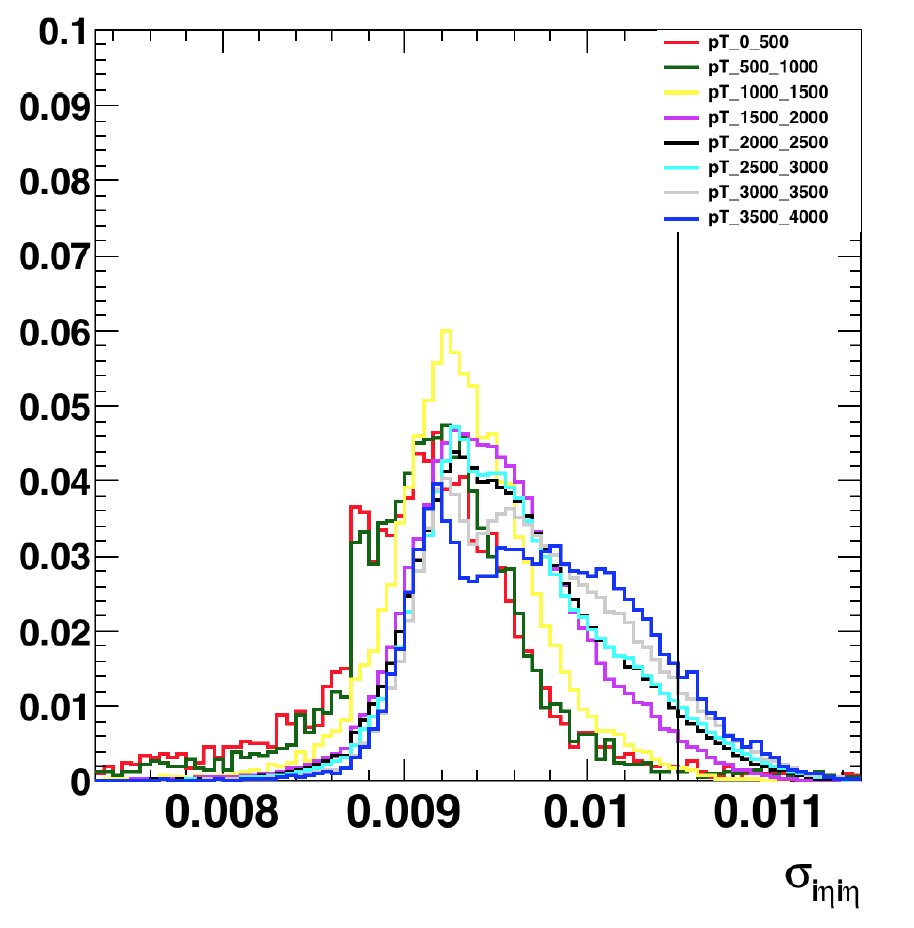
\includegraphics[width=0.49\textwidth]{figures/sieie_sat_old}
	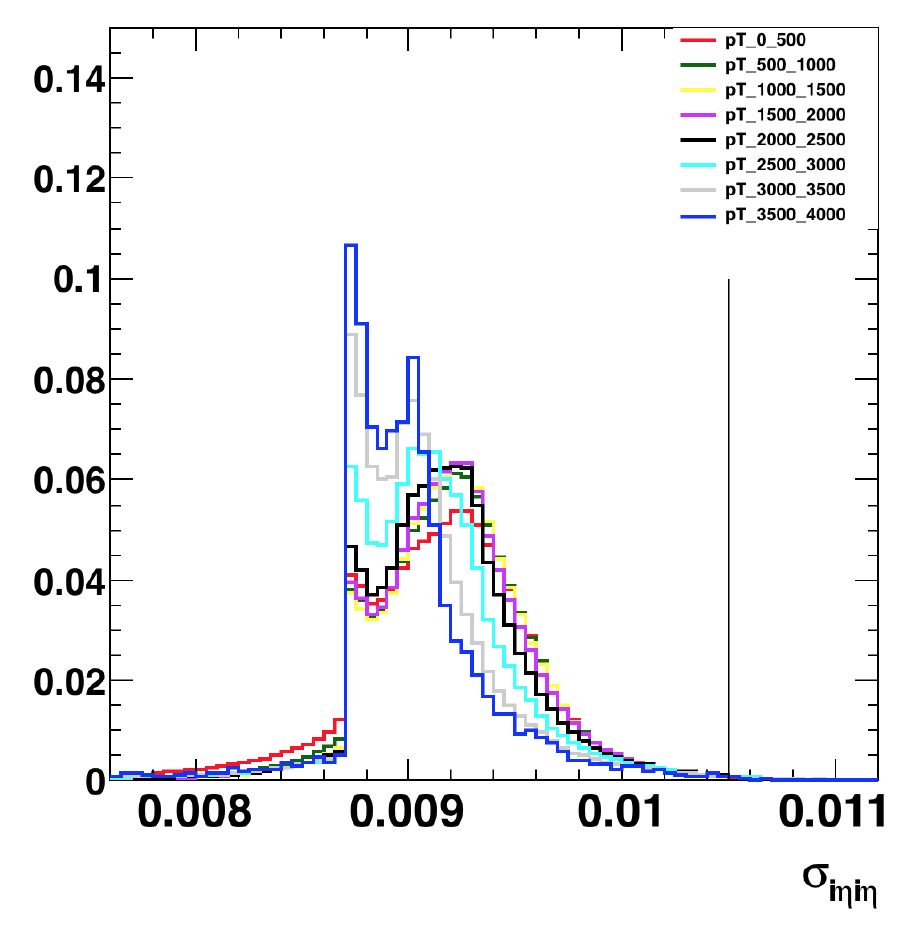
\includegraphics[width=0.49\textwidth]{figures/sieie_notSat_old}
	\caption{A plot of \sieie in various photon \pt bins for saturated (left) and unsaturated photons (right) in the EB. The vertical line is at the value of 0.0105.}
	\label{fig:sieie_sat}
\end{figure}

The variable \hoe, as defined above in Section~\ref{sec:trigger}, is the ratio of the hadronic to electromagnetic energy fraction of the photon candidate. This variable is close to zero for prompt photons, as the photon shower is well contained in the ECAL with little leakage into the HCAL. The \rnine variable is defined as the energy sum of the $3{\times}3$ array of crystals centered on the seed crystal divided by the energy of the supercluster. \rnine is sensitive to photon conversions, with unconverted photons having high values.

Isolation variables are based on the total scalar \pt sum of PF candidates assigned to the selected vertex with coordinates $(\eta,\,\phi)$ reconstructed within a cone of size $\DR = 0.3$ around the photon candidate with coordinates $(\eta_\gamma,\,\phi_\gamma)$, where $\DR = \sqrt{\smash[b]{(\eta - \eta_\gamma)^2 +(\phi-\phi_\gamma)^2}}$. In cases where the PF candidates share part of their energy with the photon candidate, they are excluded from the isolation sums. Separate variables are constructed for PF charged hadrons (\chiso) and PF photons (\phoiso). Prompt photons are well isolated for both variables. These PF candidates are calculated with respect to the diphoton vertex chosen using the $\mathrm{H} \to \gamma\gamma$ BDT. The \phoiso variable was found to be sensitive to both pileup and photon \pt. The corrected photon isolation has been pileup subtracted with \pt dependence removed according to:
\begin{equation}
	\corphoiso = \alpha + \phoiso - \rho A - \kappa \pt
\end{equation}
where $\kappa$ is a coefficient governing the \pt dependence; $\rho$ is the average pileup $\pt$ flow density per unit area in the event, calculated using the jet area method~\cite{Cacciari:2007fd,Cacciari:2008gn}; $A$ is an effective area, which is the geometrical area of the isolation cone times an $\eta$-dependent correction factor; and $\alpha$ is an empirical constant chosen to make the corrected isolation peak near zero. General pileup removal algorithms utilized by the CMS Collaboration are found in Ref.~\cite{CMS-PAS-JME-14-001}. The values for $\alpha$, $A$, and $\kappa$ are listed in Table~\ref{tab:corphoiso_values} based on the $\eta$ coordinate of the supercluster (\scEta). When \corphoiso is considered in simulated data, an additional stochastic correction is applied to account for the mismodeling of the pileup dependence of \phoiso in simulation. This correction assumes that the effect of pileup on \phoiso is to add a discrete number of photons in its isolation cone.

\begin{table}[!htbp]
	\centering
	\caption{Parameters used in the definition of \corphoiso based on the $\eta$ coordinate of the supercluster (\scEta).}
	\vspace{\baselineskip}
	\begin{tabular}{l|ccc}
	\hline \hline
	Detector region       & $\alpha$ ({\GeVns}) & $A$ & $\kappa$ \\
	\hline
	$|\scEta|<0.9$        & 0.99 & 0.15  & 0.0016 \\
	$0.9<|\scEta|<1.4442$ & 0.99 & 0.13  & 0.0016 \\
	$1.566<|\scEta|<2.0$  & 0.77 & 0.093 & 0.00075  \\
	$2.0<|\scEta|<2.2$    & 0.77 & 0.15  & 0.00075  \\
	$2.2<|\scEta|<2.5$    & 0.77 & 0.21  & 0.00075  \\
	\hline \hline
	\end{tabular}
	\label{tab:corphoiso_values}
\end{table}

Electrons and photons leave similar energy deposits in the ECAL, so an electron veto is applied to reject electrons in the selection. Electrons are vetoed based on hits in the silicon pixel and strip trackers with a further check to ensure photon candidates associated with electron tracks are incompatible with those resulting from photon conversions. This is known as the conversion-safe electron veto (CSEV).

The cut values applied to each of these identification variables are listed in Table~\ref{tab:photon_ID}, separately for photons in the EB and EEs. This collection of photon identification criteria is known as the high-\pt photon ID. \correction{This ID was developed and tuned specifically for this analysis, with significant contributions from the author of this dissertation.}


\begin{table}[!htbp]
	\caption{The high-\pt photon ID. The cut values are listed for the different identification variables. For \sieie, the values in parenthesis correspond to saturated photons in the ECAL.}
	\centering
	\vspace{\baselineskip}
	\begin{tabular}{c|cccccc}
		\hline \hline
		\vspace*{-4.5mm} & & & & & \\
		\vspace*{+0.1mm}Photon category & \chiso ({\GeVns}) & \corphoiso ({\GeVns}) & \hoe & \sieie & \rnine & CSEV \\
		\hline
		EB & 5 & 2.75 & 0.05 & 0.0105 (0.0112) & 0.8 & applied \\
		EE & 5 & 2.0  & 0.05 & 0.028 (0.030) & 0.8 & applied \\ 
		\hline \hline
	\end{tabular}
	\label{tab:photon_ID}
\end{table}

The background which remains from misidentifications not suppressed by the high-\pt photon ID is discussed in Section~\ref{sec:fake_background}.


\subsection{Selection Efficiency}

The efficiency of the high-\pt photon ID was measured using the tag-and-probe technique, similar to the procedure done in Ref.~\cite{CMS:2011aa}. This technique is used in both data, using a sample of electron-triggered events, and in simulation, using a $Z \to e^+ e^-$ sample. The tag is an electron required to be in the event, with $\pt > 30\GeV$, passing the standard CMS electron ID. The probe is a photon with $\pt > 20\GeV$ passing the high-\pt photon ID with an inverted CSEV. The invariant mass of the tag-and-probe system is required to be between 70-110\GeV. Figure~\ref{fig:tnp_eff} shows the photon selection in the EB and EE regions, including data-over-simulation scale factors. The overall efficiency is about 90 (87)\% for single photons in the EB (EE) region. The scale factors are compatible with unity, but are still applied to the simulation described in Chapters~\ref{ch:background}~and~\ref{ch:signal}.

\begin{figure}[!htbp]
	\centering
  	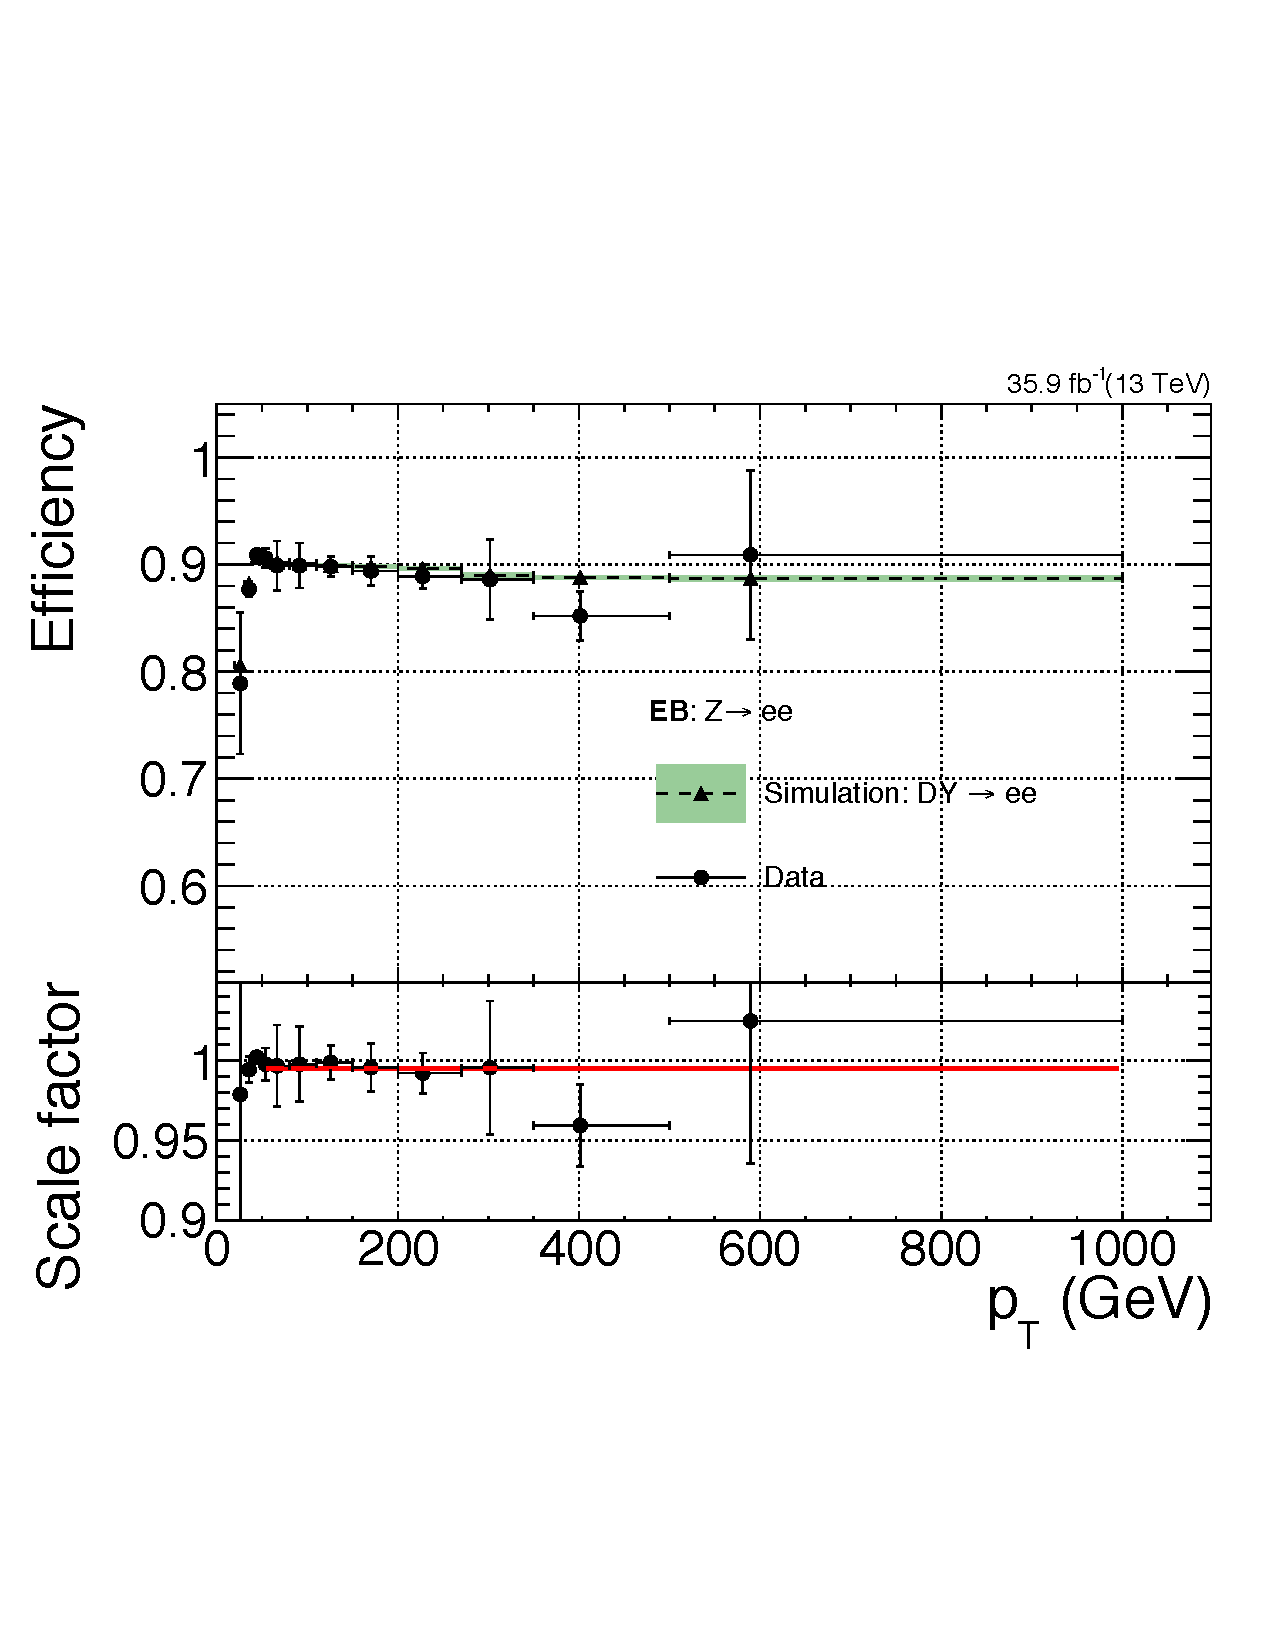
\includegraphics[angle=0,width=0.49\textwidth]{figures/sf_vs_pt_EB2.pdf}
	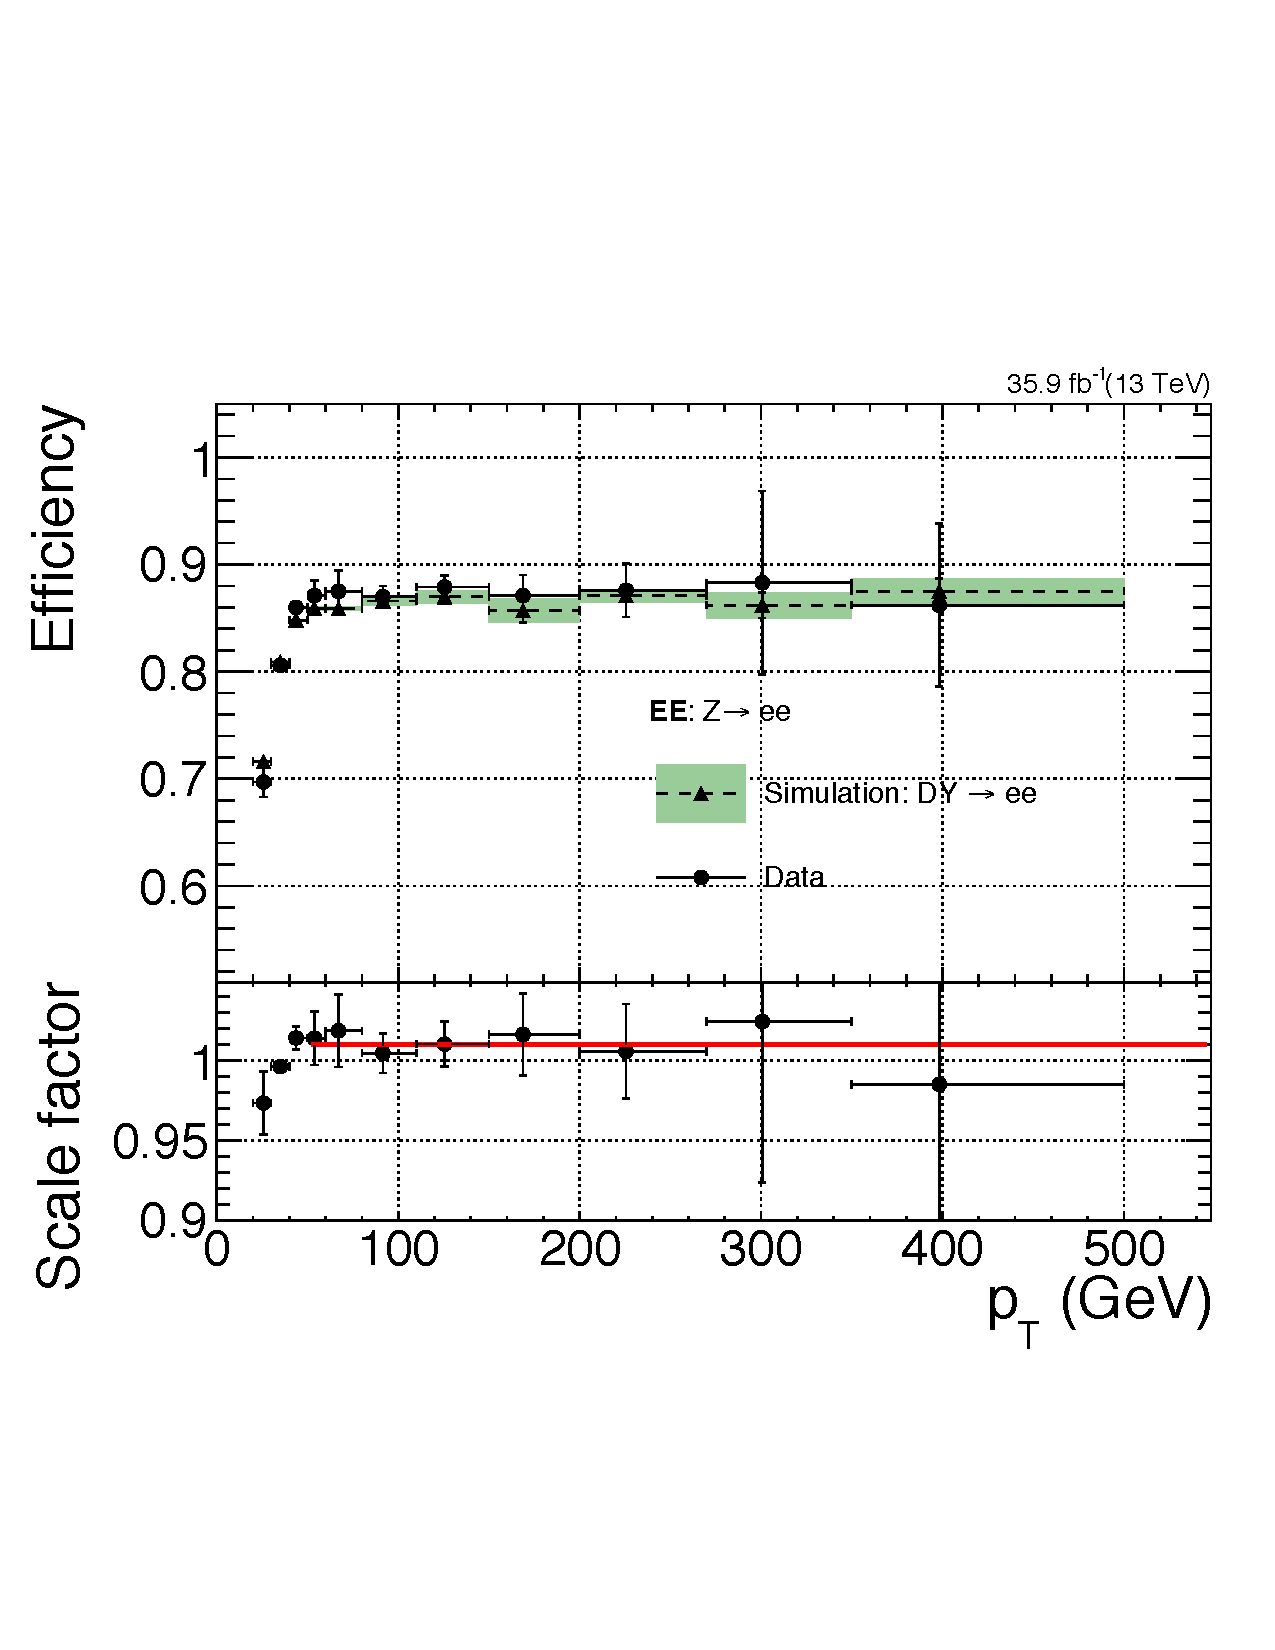
\includegraphics[angle=0,width=0.49\textwidth]{figures/sf_vs_pt_EE2.pdf}
	\caption{Photon selection efficiency (top) in the EB (left) and EE (right) regions and the associated data-over-simulation scale factors (bottom). The statistical and systematic errors are shown.}
	\label{fig:tnp_eff}
\end{figure}

The result of considering the event selection efficiency ($\varepsilon$) and detector acceptance ($A$) together is shown in Fig.~\ref{fig:eff_x_acc}. This was measured using simulation, similar to the samples described in Chapter~\ref{ch:signal}, using events of known \mgg and determining which accepted events pass the high-\pt ID requirements. The combination of each across both analysis categories is approximately 60\%.

\begin{figure}[!htb]
    \centering
    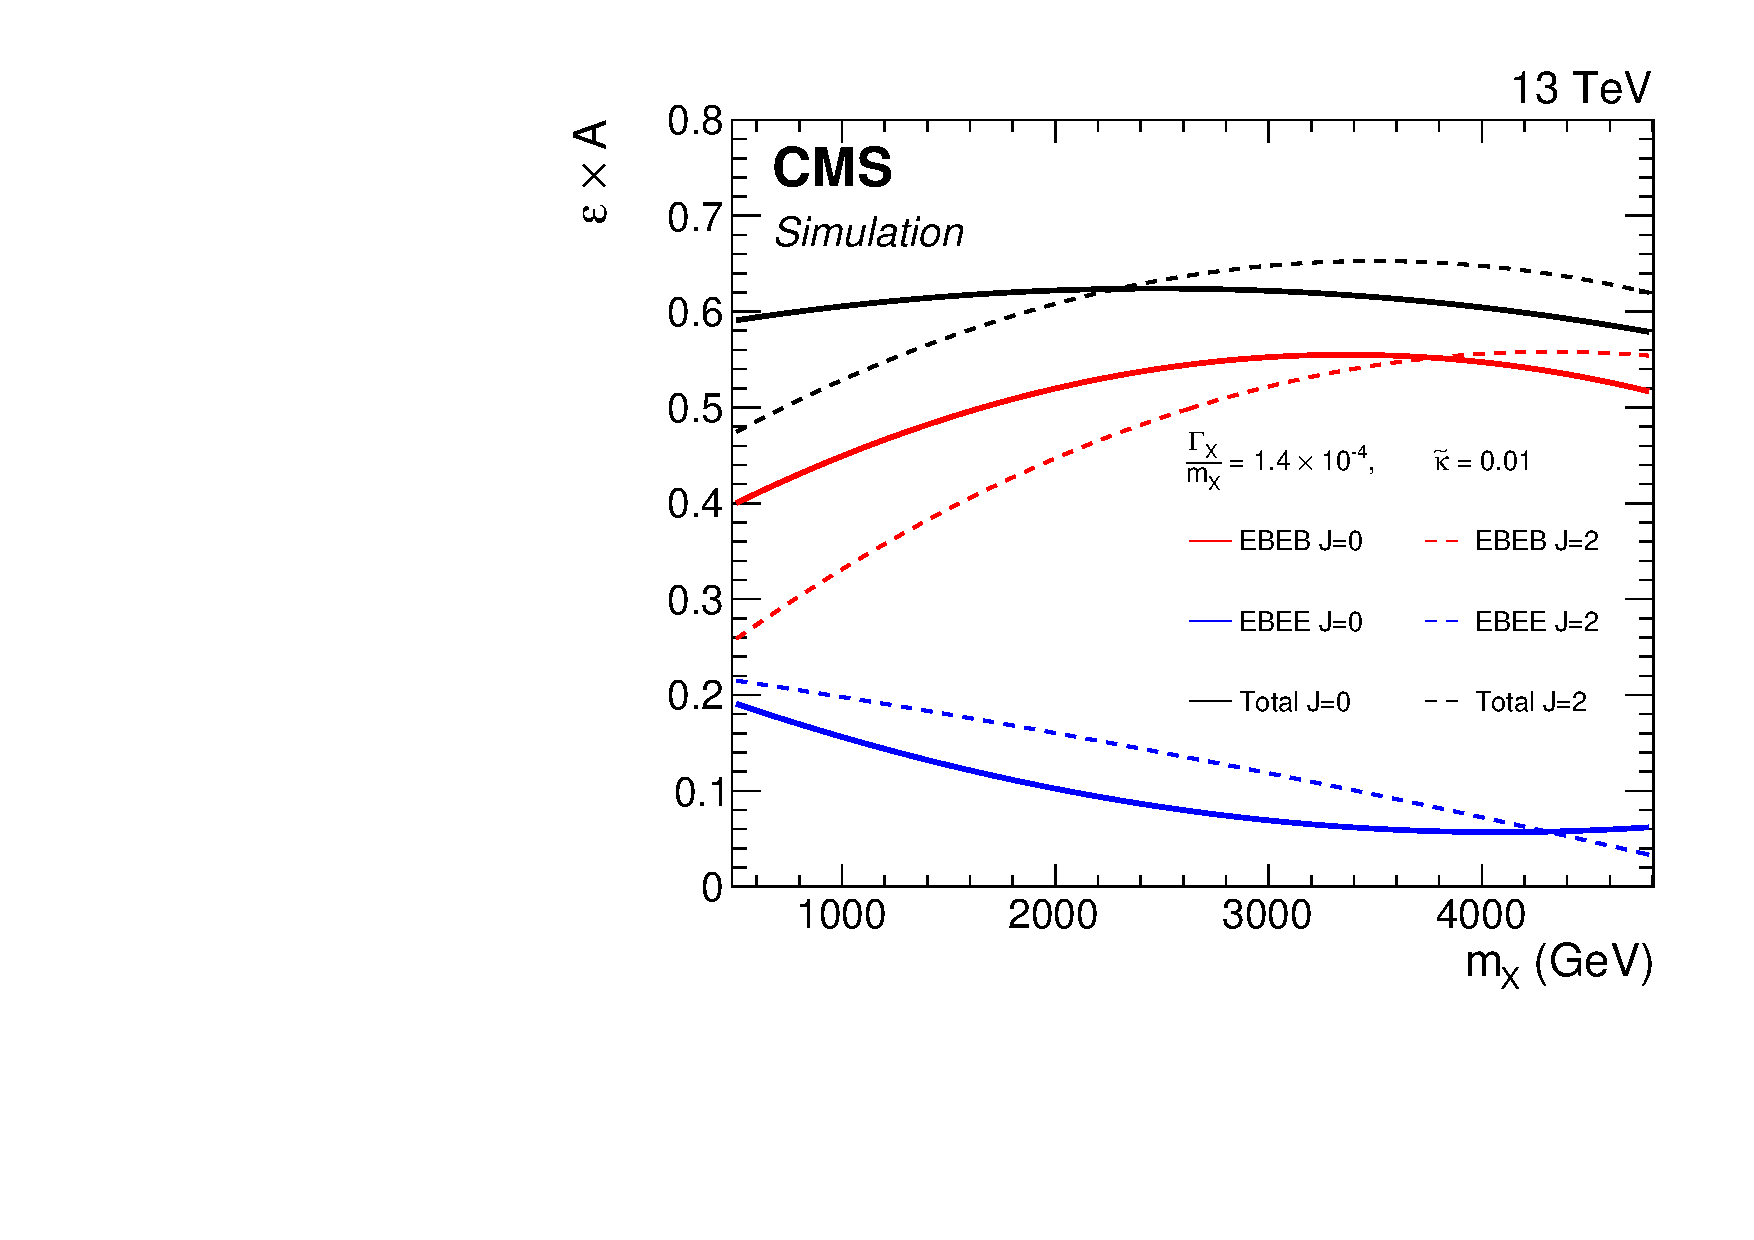
\includegraphics[width=0.65\textwidth]{figures/eff_x_acc_k001.pdf}
    \caption{The product of the event selection efficiency ($\varepsilon$) and the detector acceptance (A) is shown as a function of signal resonance mass $m_{\mathrm{X}} = \mgg$ for the $\Gamma_{\mathrm{X}}/m_{\mathrm{X}}=1.4\times10^{-4}$ signal width hypothesis. The total (black), EBEB (red), and EBEE (blue) curves are shown for the spin (J) hypotheses $\mathrm{J}=0$ (solid line) and $\mathrm{J}=2$ (dashed line).
    }
    \label{fig:eff_x_acc}
\end{figure}


\subsection{Datasets}

The datasets used in this analysis were recorded in 2016 and correspond to an integrated luminosity of 35.9\fbinv. They were produced using LHC proton-proton collisions at $\sqrt{s} = 13\TeV$ and recorded by the CMS detector. Each dataset is listed in Table~\ref{tab:data_samples} according to their internal CMS path and corresponding integrated luminosity. These \texttt{DoubleEG} triggered primary datasets contain at least two electron or photon candidates.

\begin{table}[!htbp]
	\caption{The analysis datasets, each listed with their CMS path name and corresponding integrated luminosity.}
	\centering
	\vspace{\baselineskip}
	\begin{tabular}{lc}
	\hline \hline
	Dataset path & Int. lumi.  (\fbinv) \\
	\hline
	/DoubleEG/Run2016B-03Feb2017\_ver2-v2          &  5.788 \\
	/DoubleEG/Run2016C-03Feb2017-v1/MINIAOD        &  2.573 \\
	/DoubleEG/Run2016D-03Feb2017-v1/MINIAOD        &  4.248 \\
	/DoubleEG/Run2016E-03Feb2017-v1/MINIAOD        &  4.009 \\
	/DoubleEG/Run2016F-03Feb2017-v1/MINIAOD        &  3.102 \\
	/DoubleEG/Run2016G-03Feb2017-v1/MINIAOD        &  7.540 \\
	/DoubleEG/Run2016H-03Feb2017\_ver2-v1/MINIAOD  &  8.391 \\
	/DoubleEG/Run2016H-03Feb2017\_ver3-v1/MINIAOD  &  0.215 \\
	\hline \hline
	\end{tabular}
	\label{tab:data_samples}
\end{table}




\chapter{Background Determination}\label{ch:background}

This search is for signatures of large extra-dimensional signals, as described by the ADD model, producing a nonresonant excess of high-mass diphoton events above the SM diphoton background. A defining feature of this search is the approach used to determine its background---a technique yielding a full background prediction. The background arises from two components: the real background, which comes from prompt SM diphoton production; and the fake background, which occurs when jets are misidentified as a photons in the detector. The real background is dominant. This irreducible background is calculated using a next-to-next-to-leading order Monte Carlo calculation. The subdominant fake background is reducible and is estimated from control samples in data. 


\section{Background from SM Diphoton Production}\label{sec:real_background}

This analysis is searching for high-mass photon pairs in the region $\Mgg>500\GeV$. At the LHC, the dominant background in this search region arises from prompt SM diphoton production occurring through quark annihilation (the Born process) and gluon fusion (known as the ``box" process). The Born process dominants over the box process. The leading order (LO) Feynman diagrams for these processes are shown in Fig.~\ref{fig:sm_background_diagrams}. A $qg$-initiated process is also possible, as illustrated in Fig.~\ref{fig:NLO_pp}, but is formally higher order than the Born process and is suppressed compared to the box process due the large gluon parton distribution function (PDF), as discussed in the next section. The $\gamma\gamma$ final state of these processes is the same as the signal and, therefore, this real component of the background is irreducible. A next-to-next-to-leading order (NNLO) Monte Carlo calculation is used to determine the real background.

\begin{figure}[!htbp]
  \centering
  
\includegraphics[scale=0.55]{figures/born}
  
\includegraphics[scale=0.55]{figures/box}
  \caption{Representative Feynman diagrams for the LO SM diphoton Born (left) and box (right) processes.}
  \label{fig:sm_background_diagrams}
\end{figure}


\subsection{Monte Carlo Simulation}

Monte Carlo (MC) event generation in high-energy physics (a detailed review can be found in Section~41 of Ref.~\cite{Tanabashi:2018oca}) uses a divide and conquer philosophy. The phase space is typically split into distinct domains involving a matrix element (ME) and a parton shower (PS) calculation. The ME corresponds to the calculation of the hard interaction for specific particle processes. Cross section information is provided at this stage. The evolution of these parton-level processes through radiation and fragmentation is then handled in the PS calculation. A full event history of each particle is obtained by merging the two spaces. As quarks and gluons emerge from the collisions, they radiate gluons, which split into quark-antiquark pairs. This splitting process is known as fragmentation and is dominated by the emission of soft and collinear radiation until the scale $\Lambda_{\mathrm{QCD}}$ is reached and the partons become confined into hadrons, a process known as hadronization. Hadronization is a non-perturbation process, described by different phenomenological models. For the real background calculation, we use \SHERPA~v.2.1.1~\cite{Gleisberg:2008ta}, a full Monte Carlo (MC) event generator capable of performing these steps. \SHERPA incorporates the cluster model~\cite{Webber:1983if,Winter:2003tt} to describe hadronization. To characterize the LHC proton-proton collisions, \SHERPA is embedded with the CT10 set of PDFs~\cite{Lai:2010vv,Gao:2013xoa}.

The PDF allows us to assign a fraction $x$, called the the Bjorken $x$ variable, of the total proton momentum to the colliding partons within each proton. The PDF $f_{a/A}(x_a,\mu_f^2)$ describes the probability that a parton $a$ within some hadron $A$ carries the fraction $x_a$ of the total hadron momentum, where $\mu_f$ is the factorization scale, which, roughly, separates the long- and short-distance processes. Recall, that at short distances, or equivalently high energies, QCD is perturbative, allowing these processes to be calculated, while at long distances the regime is non-perturbative. The factorization scale is usually set at the energy scale of the hard scattering interaction, $\mu_f \sim Q^2$, where $Q^2$ is the momentum transfer in the collision. The interaction cross section is found by summing over the partons and integrating the PDFs according to:
\begin{equation}
  \sigma_{AB\to X} = \sum_{a,b} \int{dx_a dx_b f_{a/A}(x_a,\mu_f^2) f_{b/B}(x_b,\mu_f^2) } \hat{\sigma}_{ab\to X}
\end{equation}
\noindent for partons $a$ and $b$, within hadrons $A$ and $B$, carrying momentum fractions $x_a$ and $x_b$, respectively, where $\hat{\sigma}_{ab\to X}$ is the parton hard scattering cross section. See Fig.~\ref{fig:pp_collision} for a diagram representing this hard scattering process. In addition to $\mu_f$, this calculation also requires the choice of the renormalization scale $\mu_r$, the scale for the QCD running coupling. Some example PDFs from the CT10 PDF set are shown in Fig.~\ref{fig:ct10_pdf}.

\begin{figure}[!htbp]
  \centering
  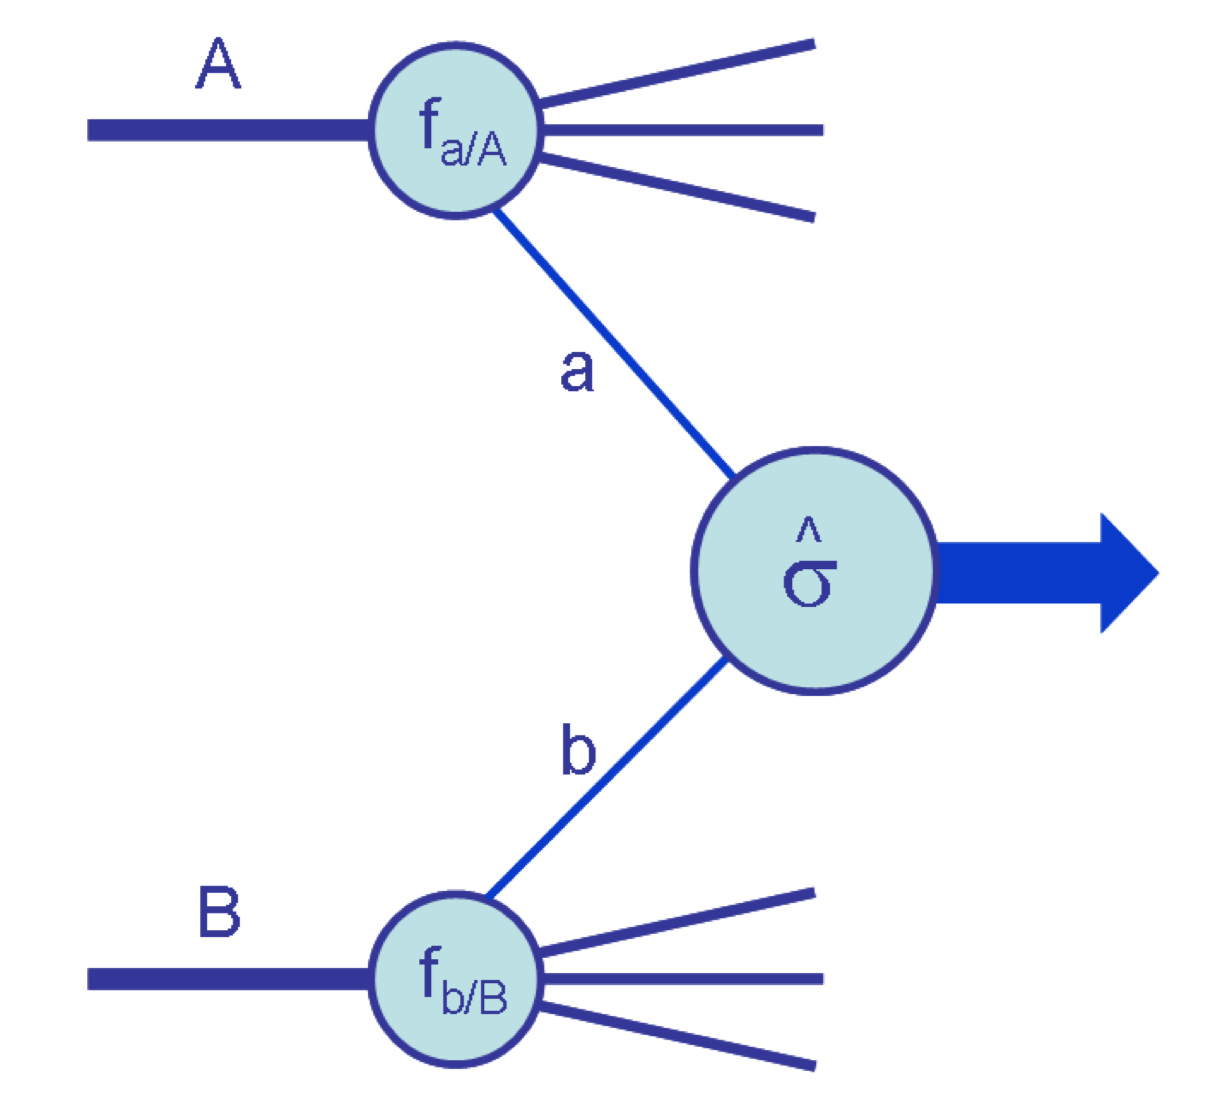
\includegraphics[scale=0.35]{figures/pp_collision}
  \caption{Diagrammatic representation of a proton-proton collision with their partons undergoing the hard scattering process~\cite{Campbell:2006wx}. The remainder of the two protons after collision is known as the beam remnant.}
  \label{fig:pp_collision}
\end{figure}

\begin{figure}[!htbp]
  \centering
  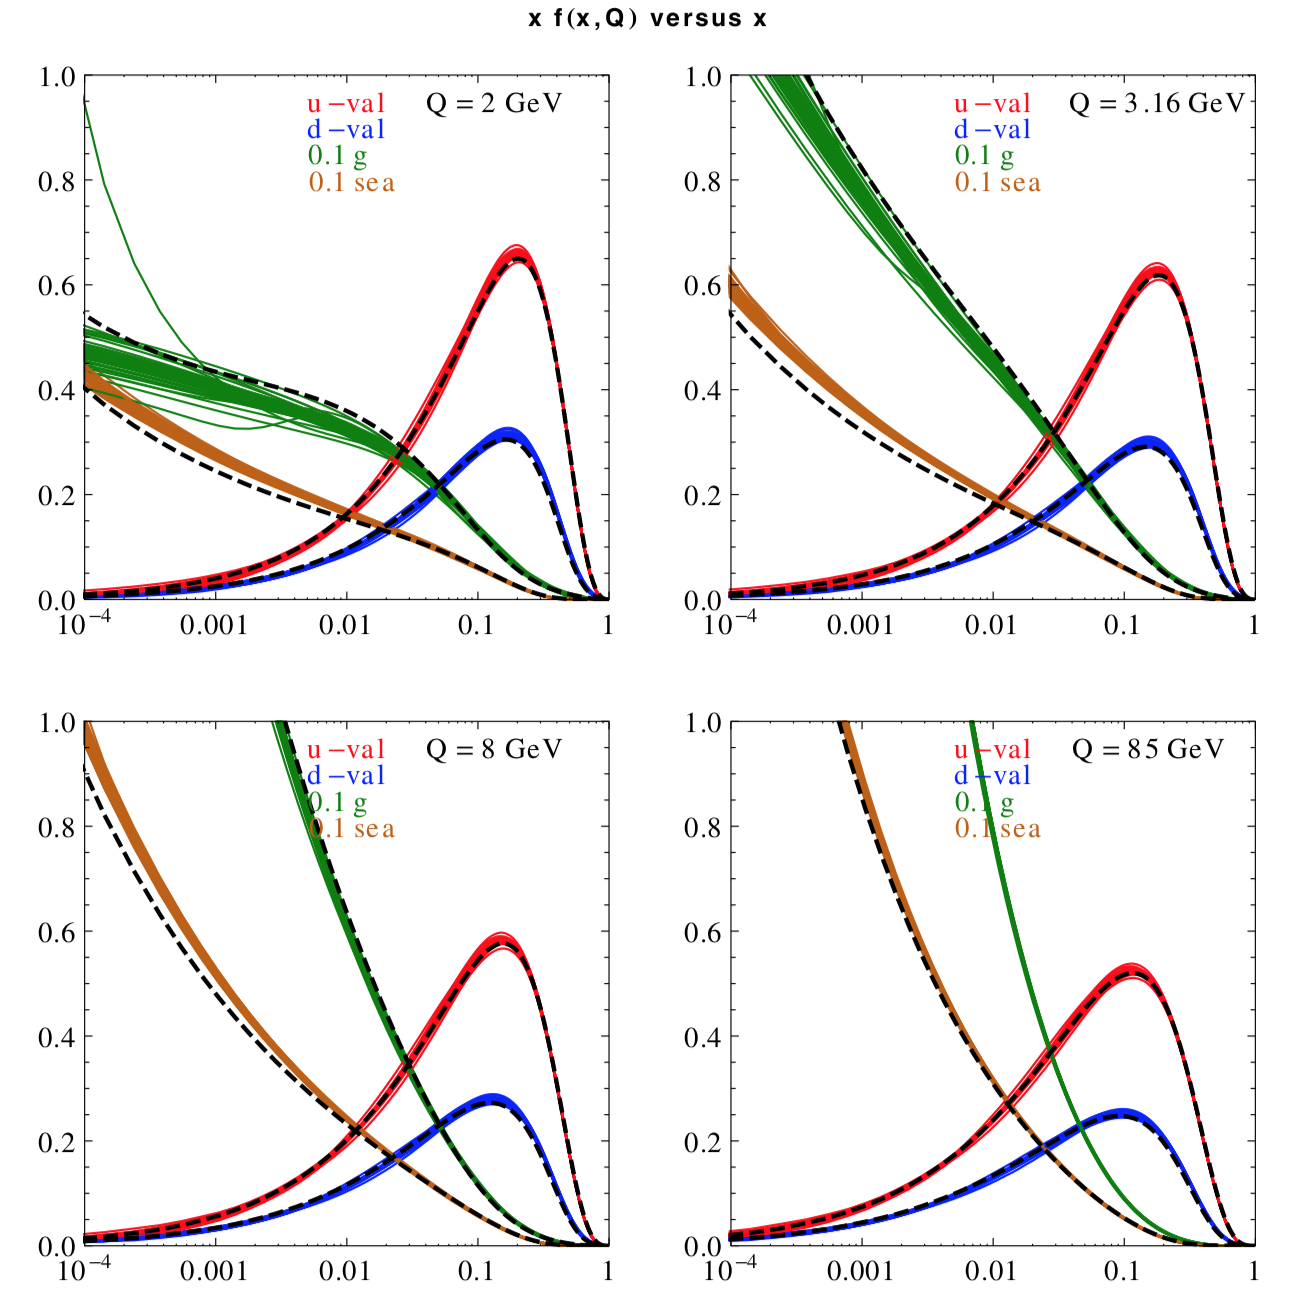
\includegraphics[scale=0.50]{figures/ct10_pdf}
  \caption{Example PDFs at energy scales $Q=2$, 3.16, 8, and 85\GeV, from the CT10 set of PDFs~\cite{Gao:2013xoa}.}
  \label{fig:ct10_pdf}
\end{figure}

\SHERPA can be configured to produced events from user specified processes generated from the proton collisions. Both the Born and box processes are included in the \SHERPA ME calculation and treated separately. The box process is calculated at the LO 1-loop level using a dedicated loop-induced ME generator. Even though the box process is formally NNLO, its contribution to the cross section is comparable to the LO terms due to the large gluon PDFs. Up to three additional final state partons are included in the Born process. Both quarks and gluons are allowed in the initial state of the Born process yielding higher order terms involving the additional final state partons through $jj\to\gamma\gamma+nj$, for a jet $j$ and integer $n=0$, 1, 2, or 3. However, \SHERPA only incorporates the real radiation component of these higher order processes and does not include virtual corrections. Fig.~\ref{fig:NLO_pp} shows some representative Feynman diagrams for NLO diphoton production in the Born process. 

\begin{figure}[hbt!]
  \centering
  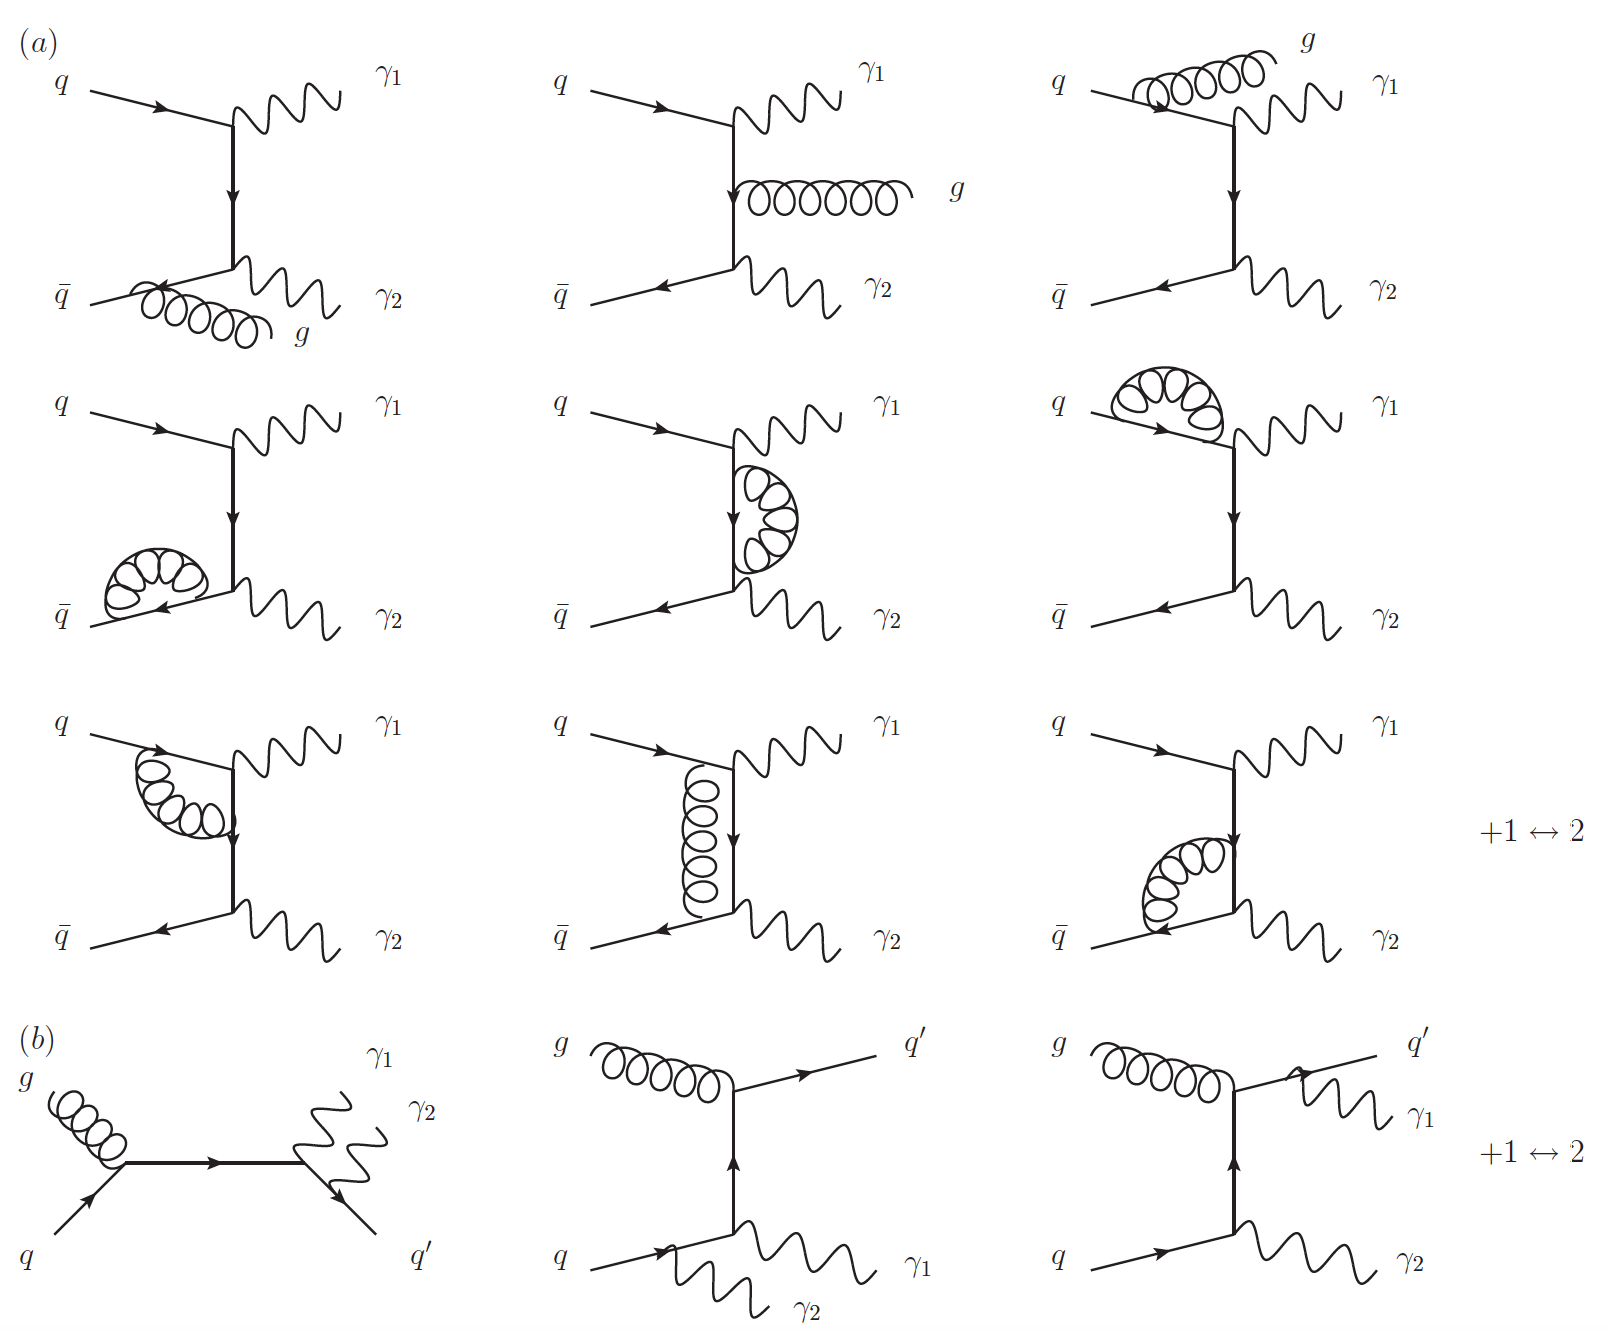
\includegraphics[scale=0.55]{figures/born_nlo}
  \caption{Representative Feynman diagrams for NLO diphoton production through the born process~\cite{DErrico:2011cgc}. In (a) $q\bar{q}$ and (b) $gq$ initiated processes are shown.}
  \label{fig:NLO_pp}
\end{figure}

The inclusion of additional final state jets is important for sampling the diphoton phase space as demonstrated in Ref.~\cite{CMS-PAS-EXO-12-045}. Here it was determined using Run 1 data that the variable $\Delta\phi_{\gamma\gamma}$, which is the difference in the $\phi$ coordinate between the two photons forming the diphoton object in the event, is sensitive to the presence of these additional jets and using a LO simulation was insufficient at accurately calculating the process. For computational convenience, the probability for producing these higher order processes is altered within \SHERPA by applying weights to the additional final state partons. This is corrected for in the final analysis by extracting the weights and undoing them when incorporating this background calculation. In addition to these specific processes, \SHERPA also interlaces photons into the QCD\texttt{+}QED PS~\cite{Hoeche:2009xc}. This provides prompt photon contributions from the fragmentation of quarks and gluons and is taken into account when estimating the fake background. Representative Feynman diagrams for this fragmentation process are shown in Fig.~\ref{fig:NLO_pp_onefrag}.

\begin{figure}[!htbp]
  \centering
  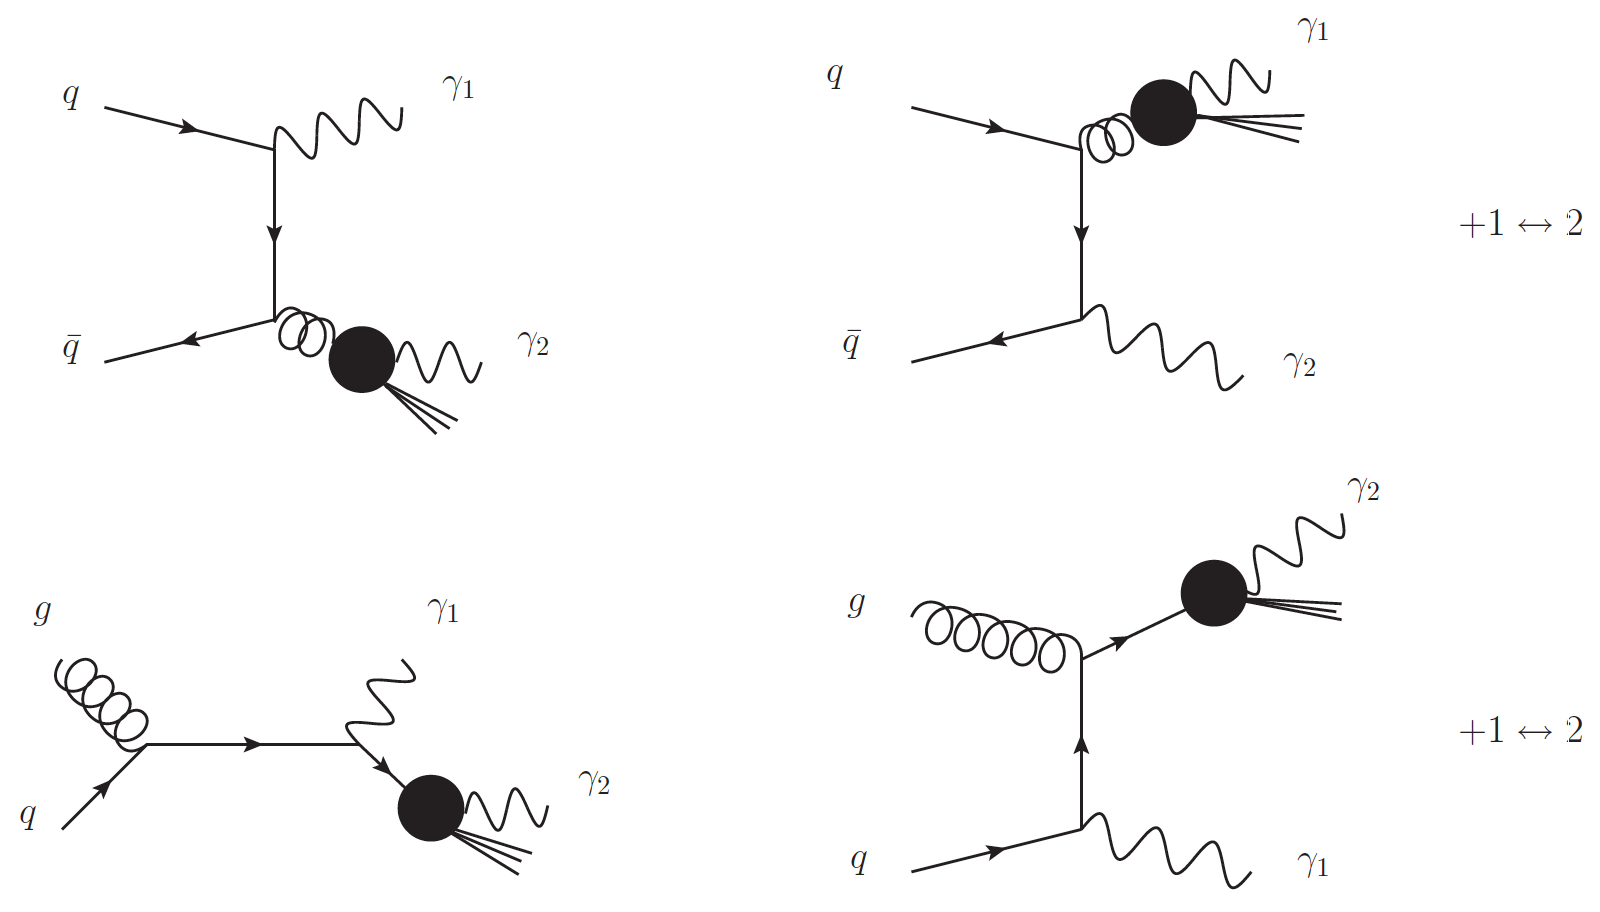
\includegraphics[scale=0.45]{figures/born_frag}
  \caption{Representative Feynman diagrams for NLO diphoton production through the fragmentation of a quark or gluon~\cite{DErrico:2011cgc}.}
  \label{fig:NLO_pp_onefrag}
\end{figure}

Within \SHERPA a kinematic selection of $\pt>50\GeV$ and $|\eta|<2.8$ is imposed on the photons during event generation. To improve statistics the event generation is broken into eight samples corresponding to the diphoton invariant mass \Mgg bins of 60-200, 200-500, 500-1000, 1000-2000, 2000-4000, 4000-6000, 6000-8000, and 8000-13000\GeV. These parameters are specified and configured in \SHERPA using run cards. An example run card used to generate one of these samples is shown in Appendix~\ref{sec:SM_run_card}. Among all samples, a total of 6,150,000 events were generated. Table~\ref{tab:ggjets_samples} summarizes the samples and their corresponding cross sections. For each sample, the interactions of the generated particles are fully simulated through the CMS detector material using \GEANTfour~\cite{Agostinelli:2002hh} and their response to the detector's electronic readout is then reconstructed. The simulation and reconstruction use CMS detector conditions that match those used during the 2016 data-taking period and include the effects of pileup from the proton-proton collisions.

\begin{table}[!htbp]
  \caption{MC background samples used in this analysis with the number of events and corresponding cross sections. The full, internal CMS path name is specified by appending the dataset path with \texttt{/RunIISummer16MiniAODv2-\allowbreak PUMoriond17\_\allowbreak 80X\_\allowbreak mcRun2\_\allowbreak asymptotic\_\allowbreak 2016\_\allowbreak TrancheIV\_\allowbreak v6/\allowbreak MINIAODSIM}.}
  \label{tab:ggjets_samples}
  \centering
  \vspace{\baselineskip}
  \begin{tabular}{lcc}
    \hline
    \hline
    Dataset path & Number of events & Cross section (pb) \\
    \hline
    /GGJets\_M-60To200\_Pt-50\_13TeV-sherpa     & 1,000,000 & 5.785     \\
    /GGJets\_M-200To500\_Pt-50\_13TeV-sherpa    & 2,500,000 & 2.244     \\
    /GGJets\_M-500To1000\_Pt-50\_13TeV-sherpa   & 1,000,000 & 1.510     \\
    /GGJets\_M-1000To2000\_Pt-50\_13TeV-sherpa  & 600,000   & 1.084e-02 \\
    /GGJets\_M-2000To4000\_Pt-50\_13TeV-sherpa  & 300,000   & 3.690e-04 \\
    /GGJets\_M-4000To6000\_Pt-50\_13TeV-sherpa  & 300,000   & 2.451e-06 \\
    /GGJets\_M-6000To8000\_Pt-50\_13TeV-sherpa  & 250,000   & 1.753e-08 \\
    /GGJets\_M-8000To13000\_Pt-50\_13TeV-sherpa & 200,000   & 7.053e-11 \\
    \hline
    \hline
  \end{tabular}
\end{table}

\correction{These \SHERPA samples contain individual events which have been fully simulated and reconstructed through the CMS detector, but higher order terms are absent. Unfortunately, at present, the MC programs capable of calculating the SM diphoton background at higher orders are not interfaced with \GEANTfour and, hence, cannot provide simulated events. However, these higher order MC programs are capable of calculating (currently, at full NNLO) the diphoton cross section at generator-level in a specified phase space, yielding distributions. \SHERPA also provides these same distributions at generator-level, allowing for a comparison. The ratio of these generator-level background predictions is called the \Kfactor. We will follow this general approach to produce a \Kfactor which will be subsequently applied to the simulation-level \SHERPA samples. This procedure allows us to reweight the simulated events, providing a full NNLO diphoton background prediction, accounting for the missing higher order terms in the original samples.}


\subsection{The \emph{K} Factor}\label{sec:k_factor}


\correction{The MC program \MCFM~8.0~\cite{Campbell:2016yrh} is capable of calculating a full NNLO diphoton cross section at generator-level and will be used to form the \Kfactor. \MCFM includes the 1-loop virtual corrections to the Born process, as shown in Fig.~\ref{fig:NLO_pp}, as well as for the box process. In addition, \MCFM includes the NNLO diagrams for the Born process and NLO diagrams for the box process in its calculation, as depicted in Figures~\ref{fig:MCFM_born_diagrams} and~\ref{fig:MCFM_box_diagrams}, respectively. \MCFM allows light fermions in the box process to circulate in the loop, but further considers the finite mass of the $t$ quark by also allowing it to circulate. The effects of this become important at high \Mgg~~\cite{Campbell:2016yrh}.}

\begin{figure}[hbt!]
  \centering
  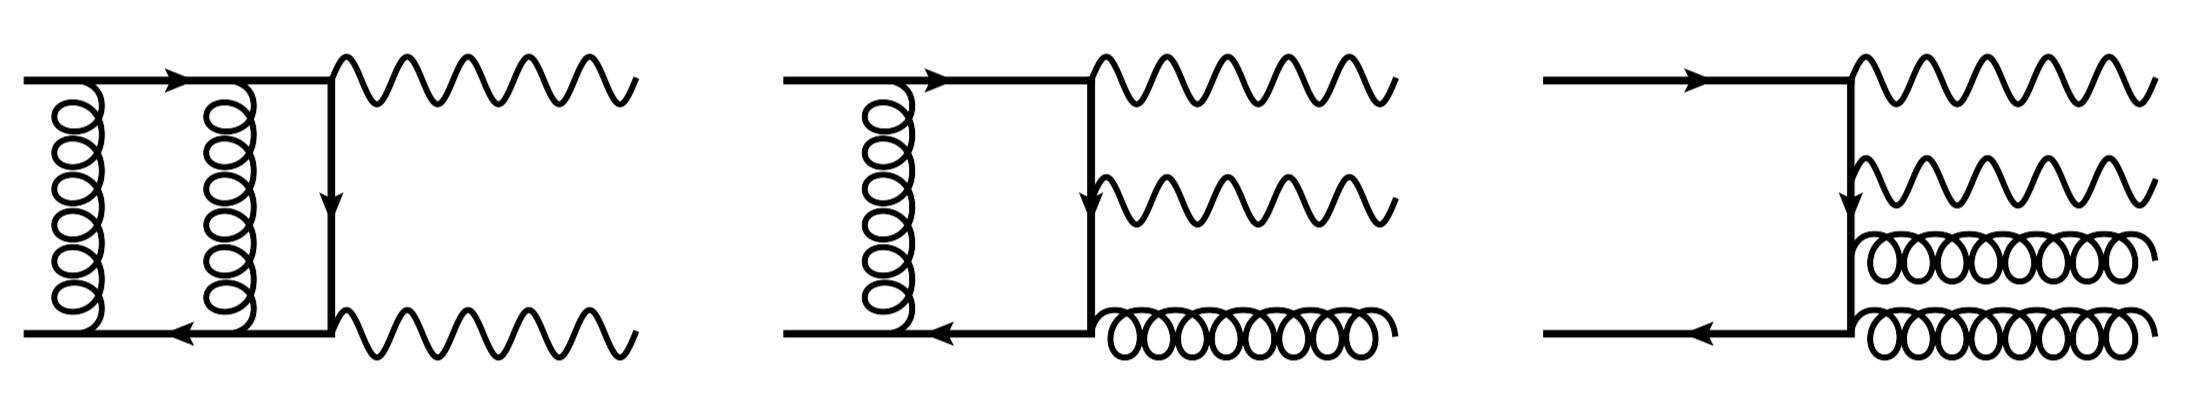
\includegraphics[scale=0.40]{figures/born_nnlo}
  \caption{Representative Feynman diagrams for the diphoton Born process at NNLO, considered by \MCFM~\cite{Campbell:2016yrh}.}
  \label{fig:MCFM_born_diagrams}
\end{figure}

\begin{figure}[hbt!]
  \centering
  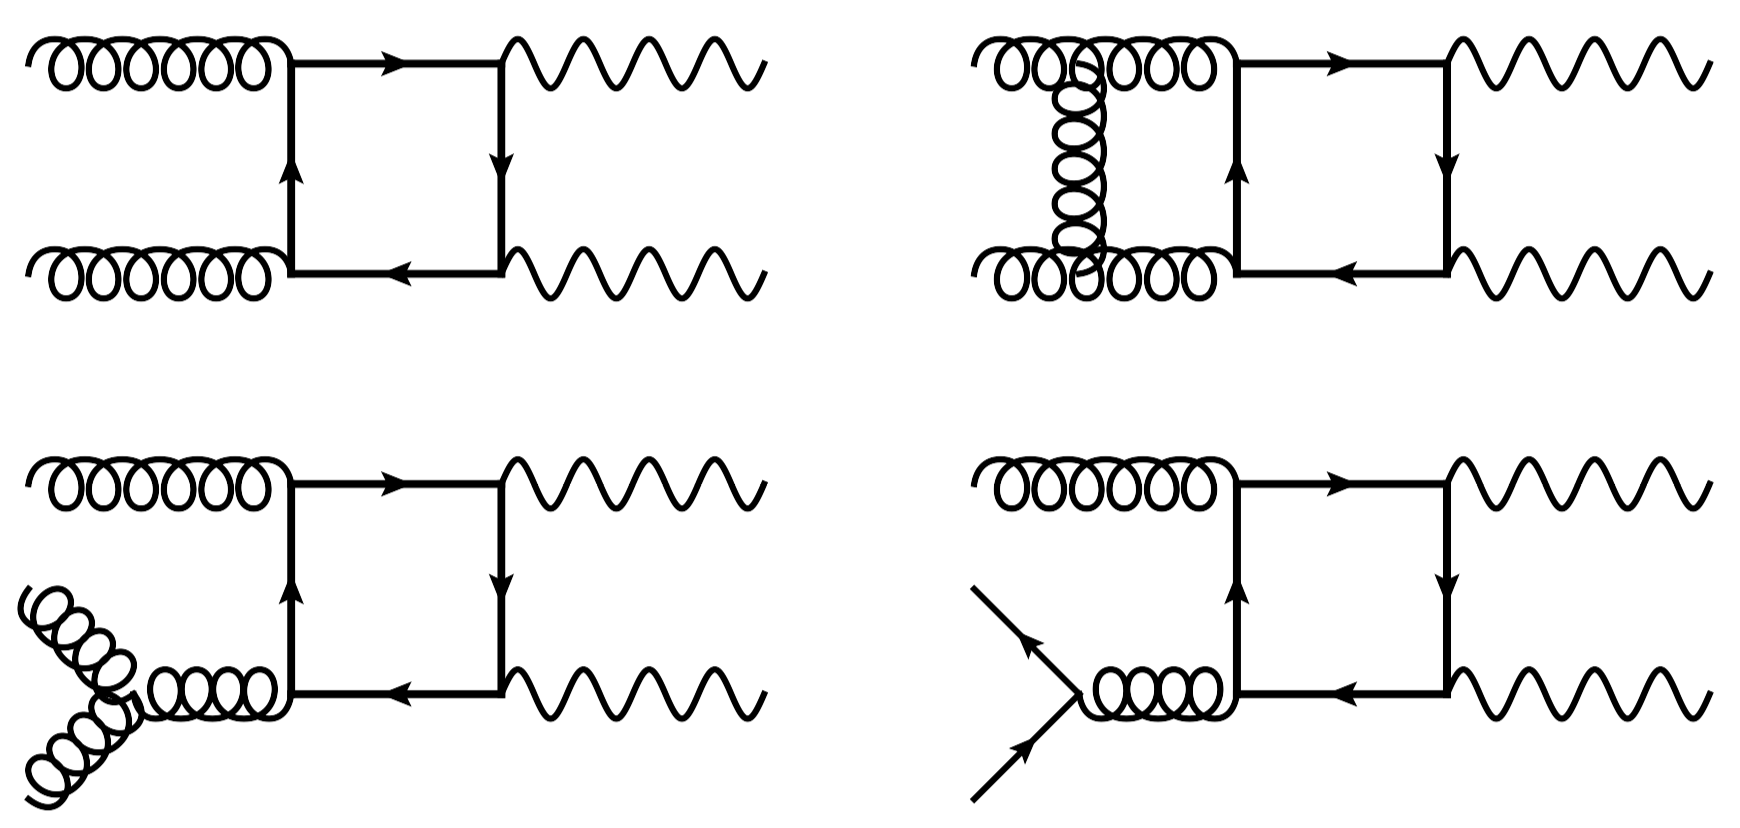
\includegraphics[scale=0.50]{figures/box_nlo}
  \caption{Representative Feynman diagrams for the diphoton box process at LO and NLO, considered by \MCFM~\cite{Campbell:2016yrh}.}
  \label{fig:MCFM_box_diagrams}
\end{figure}

\correction{For the calculation, we will interface \MCFM with the CT10 set of PDFs, as was done for the \SHERPA calculation. \MCFM can only provide parton-level cross section information for different diphoton kinematic variables, instead of individual, simulation-level events, since it is not interfaced with \GEANTfour. The NNLO contributions to the SM diphoton production processes are calculated as functions of \Mgg. Kinematic cuts are placed on the generator-level photons during the parton-level calculation. These are the same kinematic cuts used offline in the analysis, requiring photons to have $\pt>75\GeV$ and restricting them to reside within the EB or an EE using the appropriate values of photon $\eta$. Photon isolation is calculated using the method by Frixione~\cite{Frixione:1998jh}, which imposes an isolation requirement that depends on the $\Delta R$ from the location of the photon. The isolation at all distances must be within 5\GeV. Diphoton objects are then selected and categorized into the EBEB and EBEE regions. The four \Mgg bins of 500-750, 750-1000, 1000-1500, and 1500-4000\GeV are used during the calculation to improve the statistics of the overall calculation and reduce any potential statistical bias when a large range of \Mgg is separately considered. Finally, we reject events with very small $\Delta R_{\gamma\gamma}$ ($<$0.45) to avoid an infrared divergence from collinear photon emissions. \SHERPA is configured in an analogous way, providing similar diphoton cross section distributions as a function of \mgg, allowing for the formation of the \Kfactor.}

\correction{The \Kfactor is defined as the ratio of the \MCFM NNLO generator-level prediction to the \SHERPA generator-level prediction, both produced using equivalent settings. Fig.~\ref{fig:kfactor_mgg} (middle) shows the \MCFM LO (black), NLO (blue), and NNLO (red) calculations as a function of \Mgg compared against the \SHERPA generator-level prediction (magenta). The ratio plots show the \Kfactor distributions for each order with the final NNLO \Kfactor shown in red. The \Kfactor ranges from 1.4 to 2.2 (2.5) in the EBEB (EBEE) region for $\Mgg<3\TeV$.}

\begin{figure}[p]
  \centering
  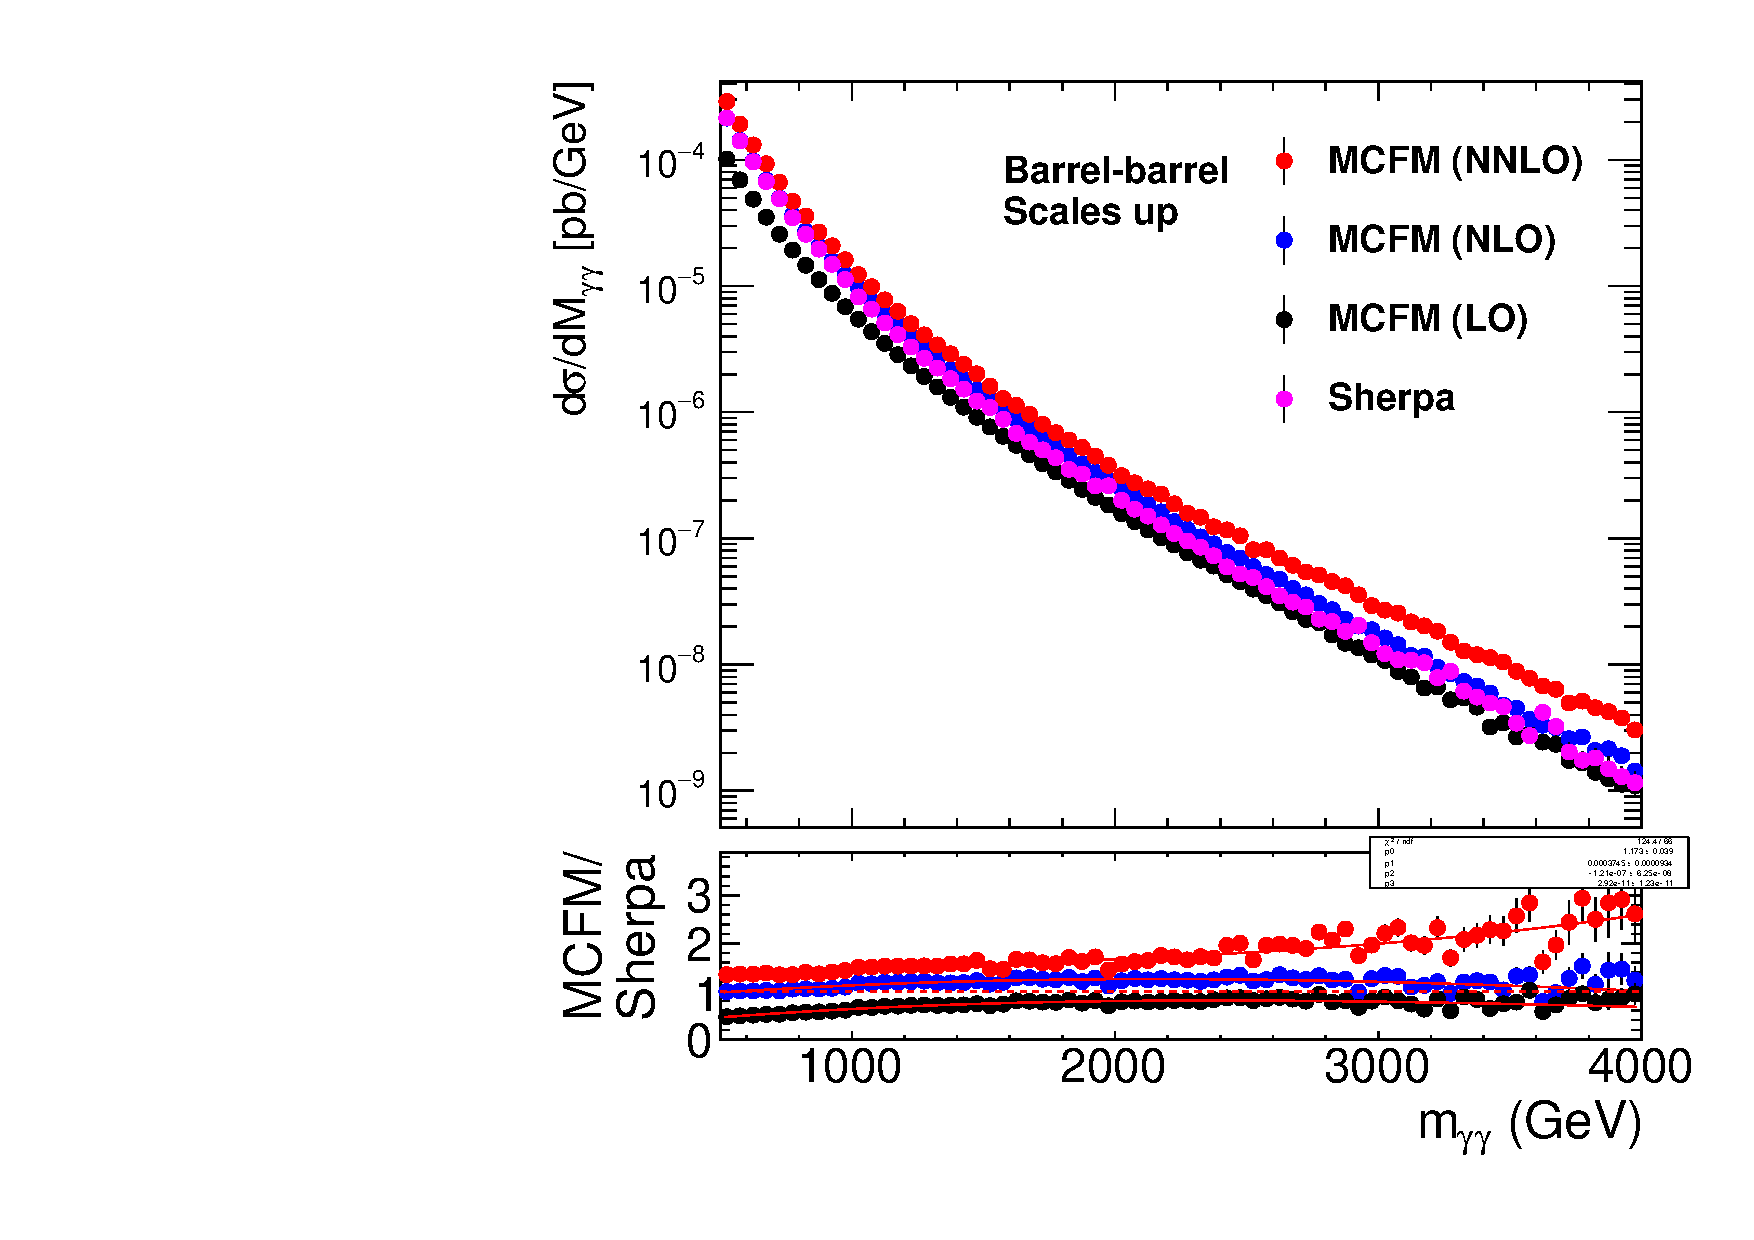
\includegraphics[angle=0,width=0.40\textwidth]{figures/BB_hist1_R2F2.pdf}
  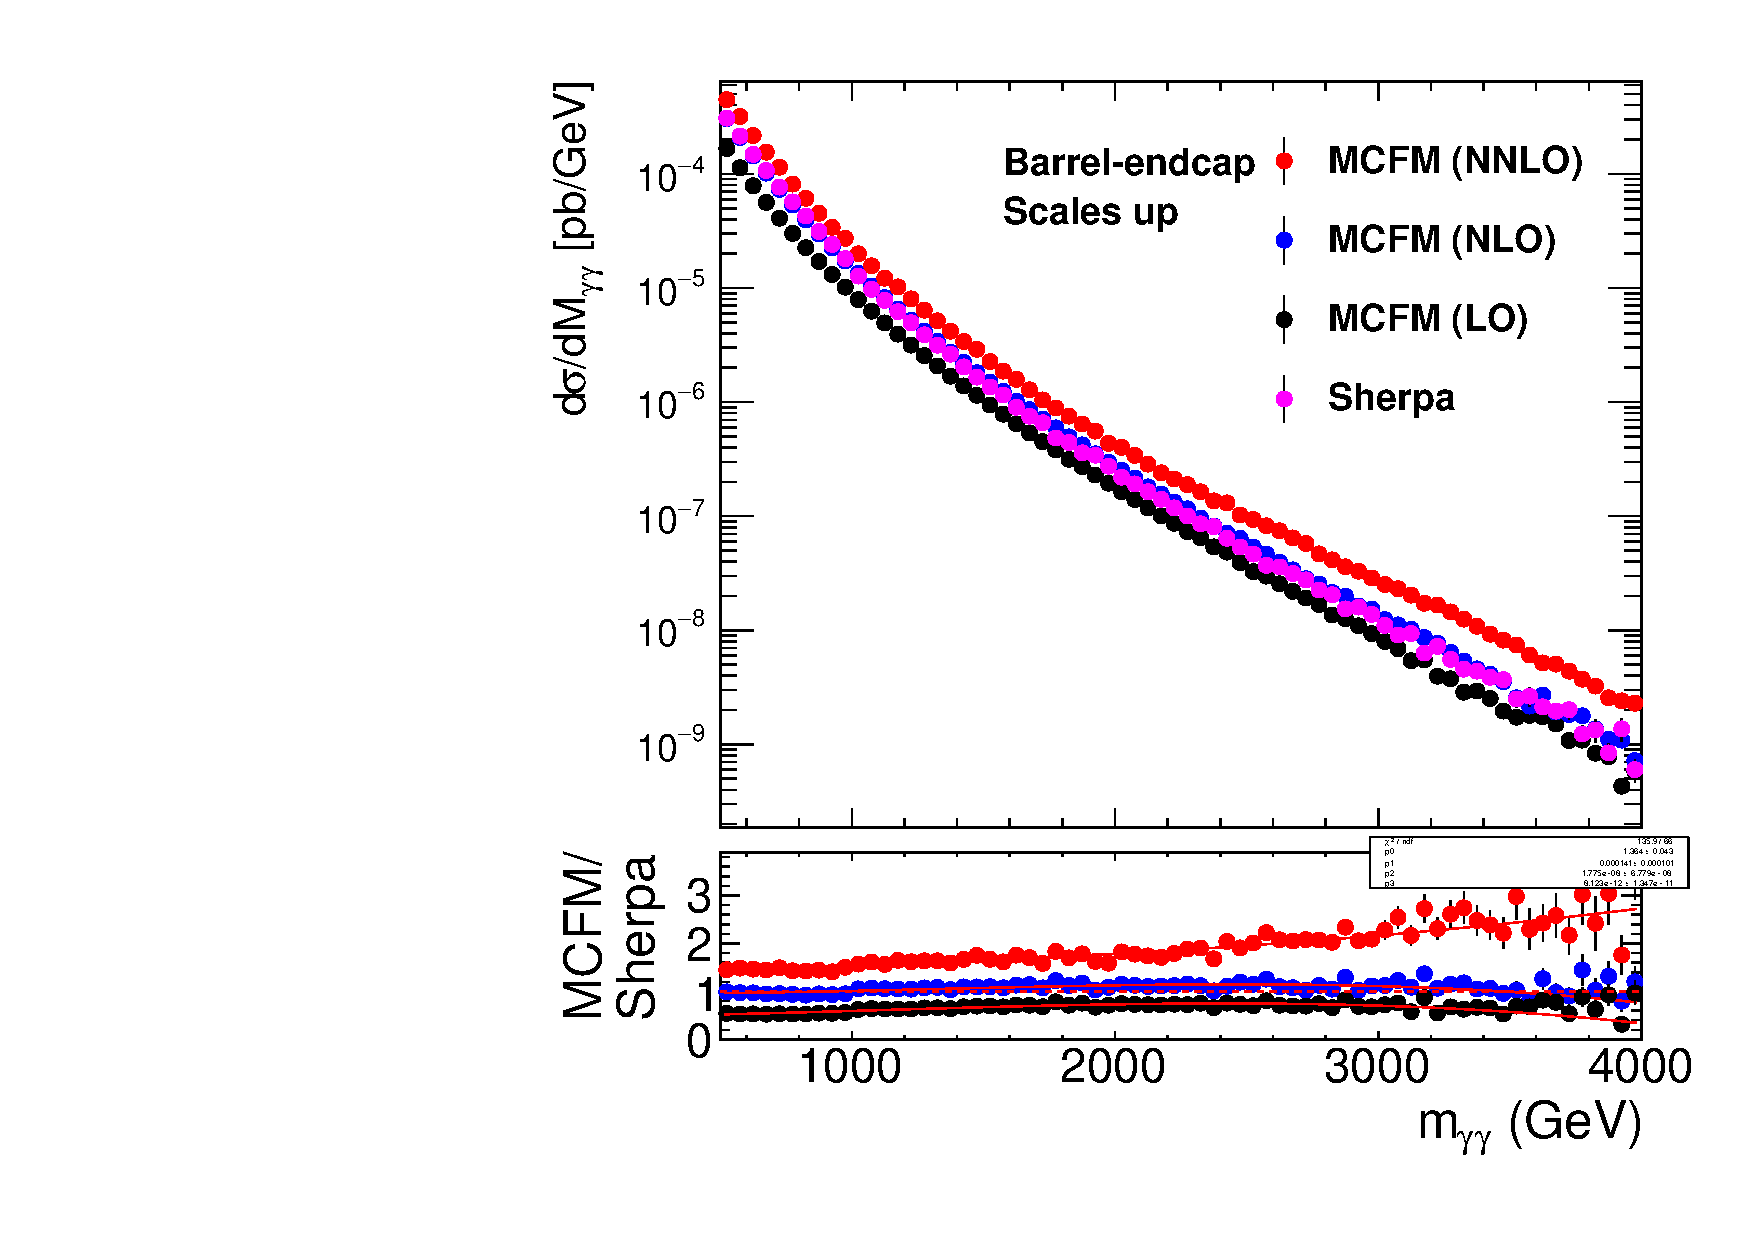
\includegraphics[angle=0,width=0.40\textwidth]{figures/BE_hist1_R2F2.pdf}
  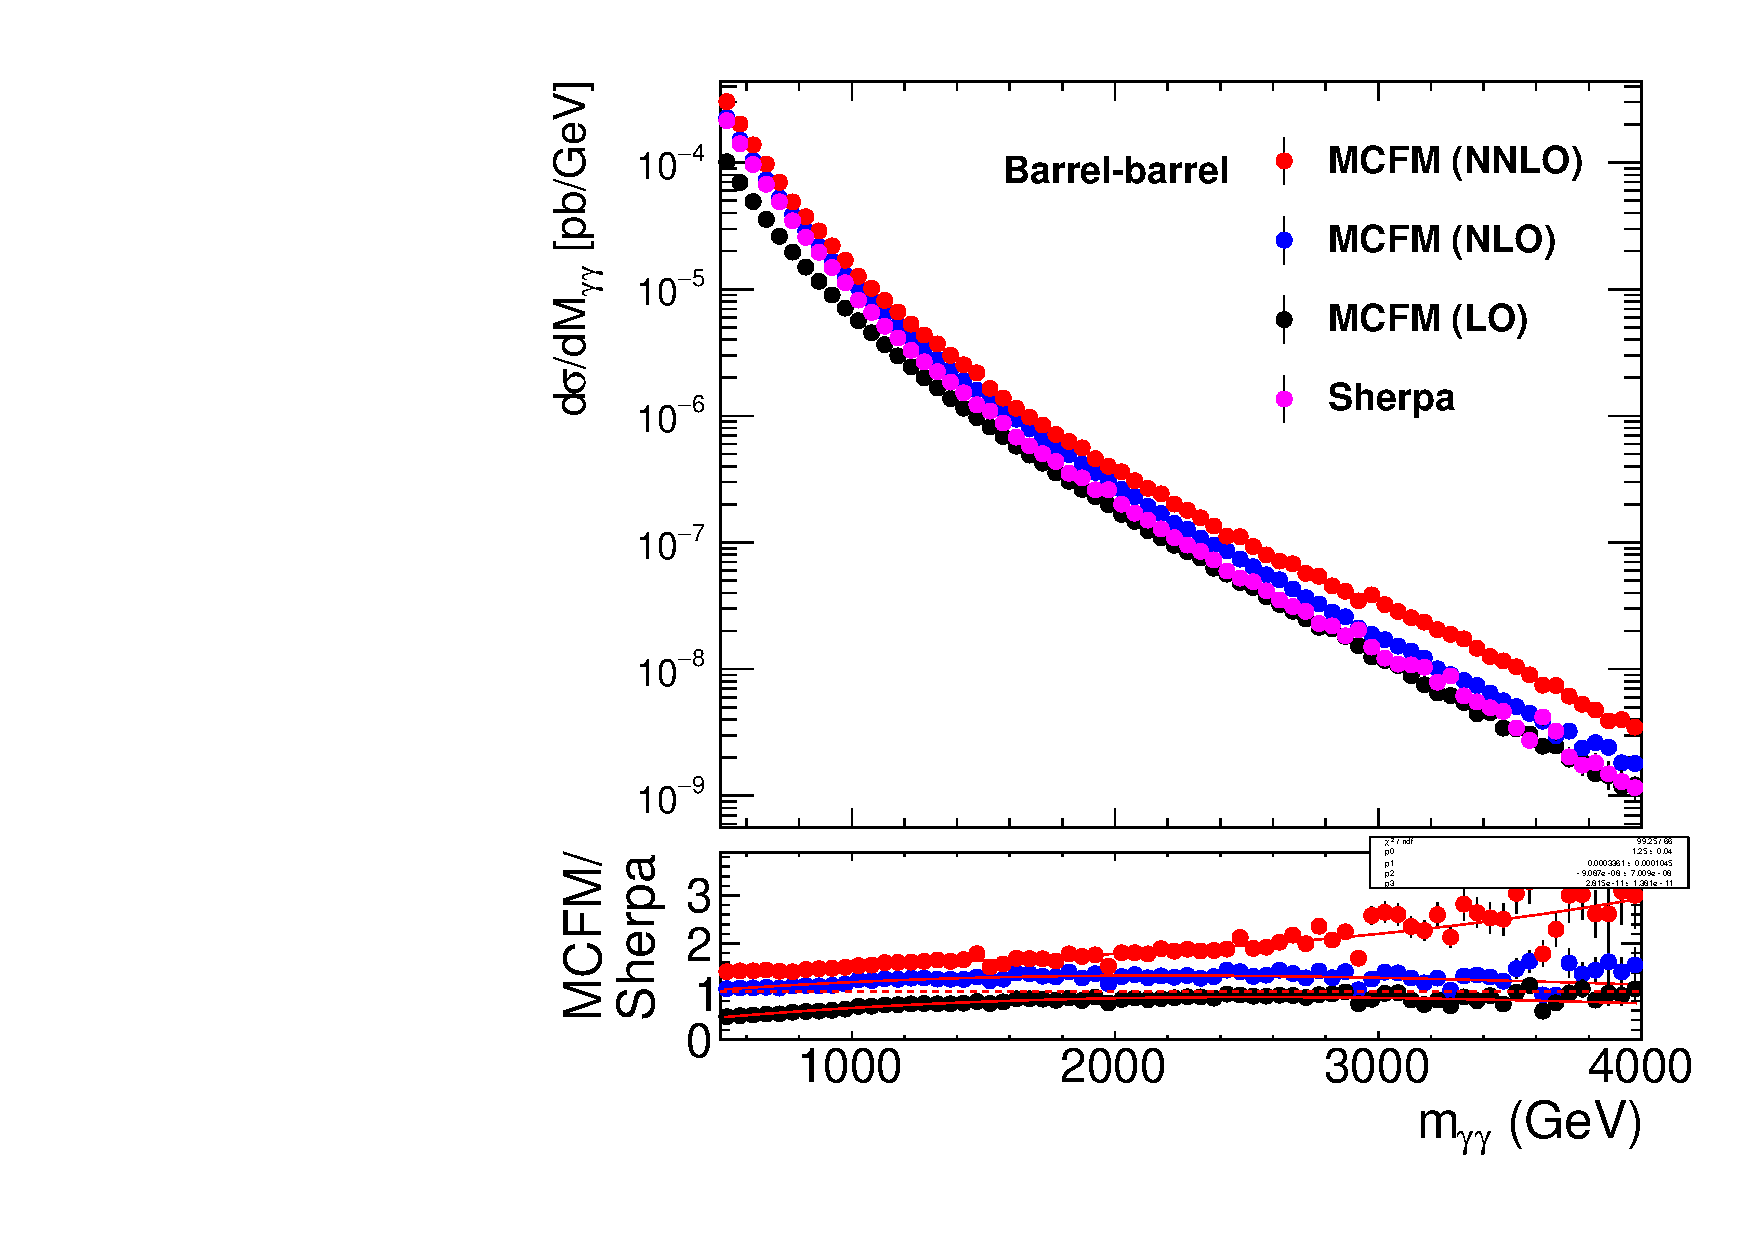
\includegraphics[angle=0,width=0.40\textwidth]{figures/BB_hist1_R1F1.pdf}
  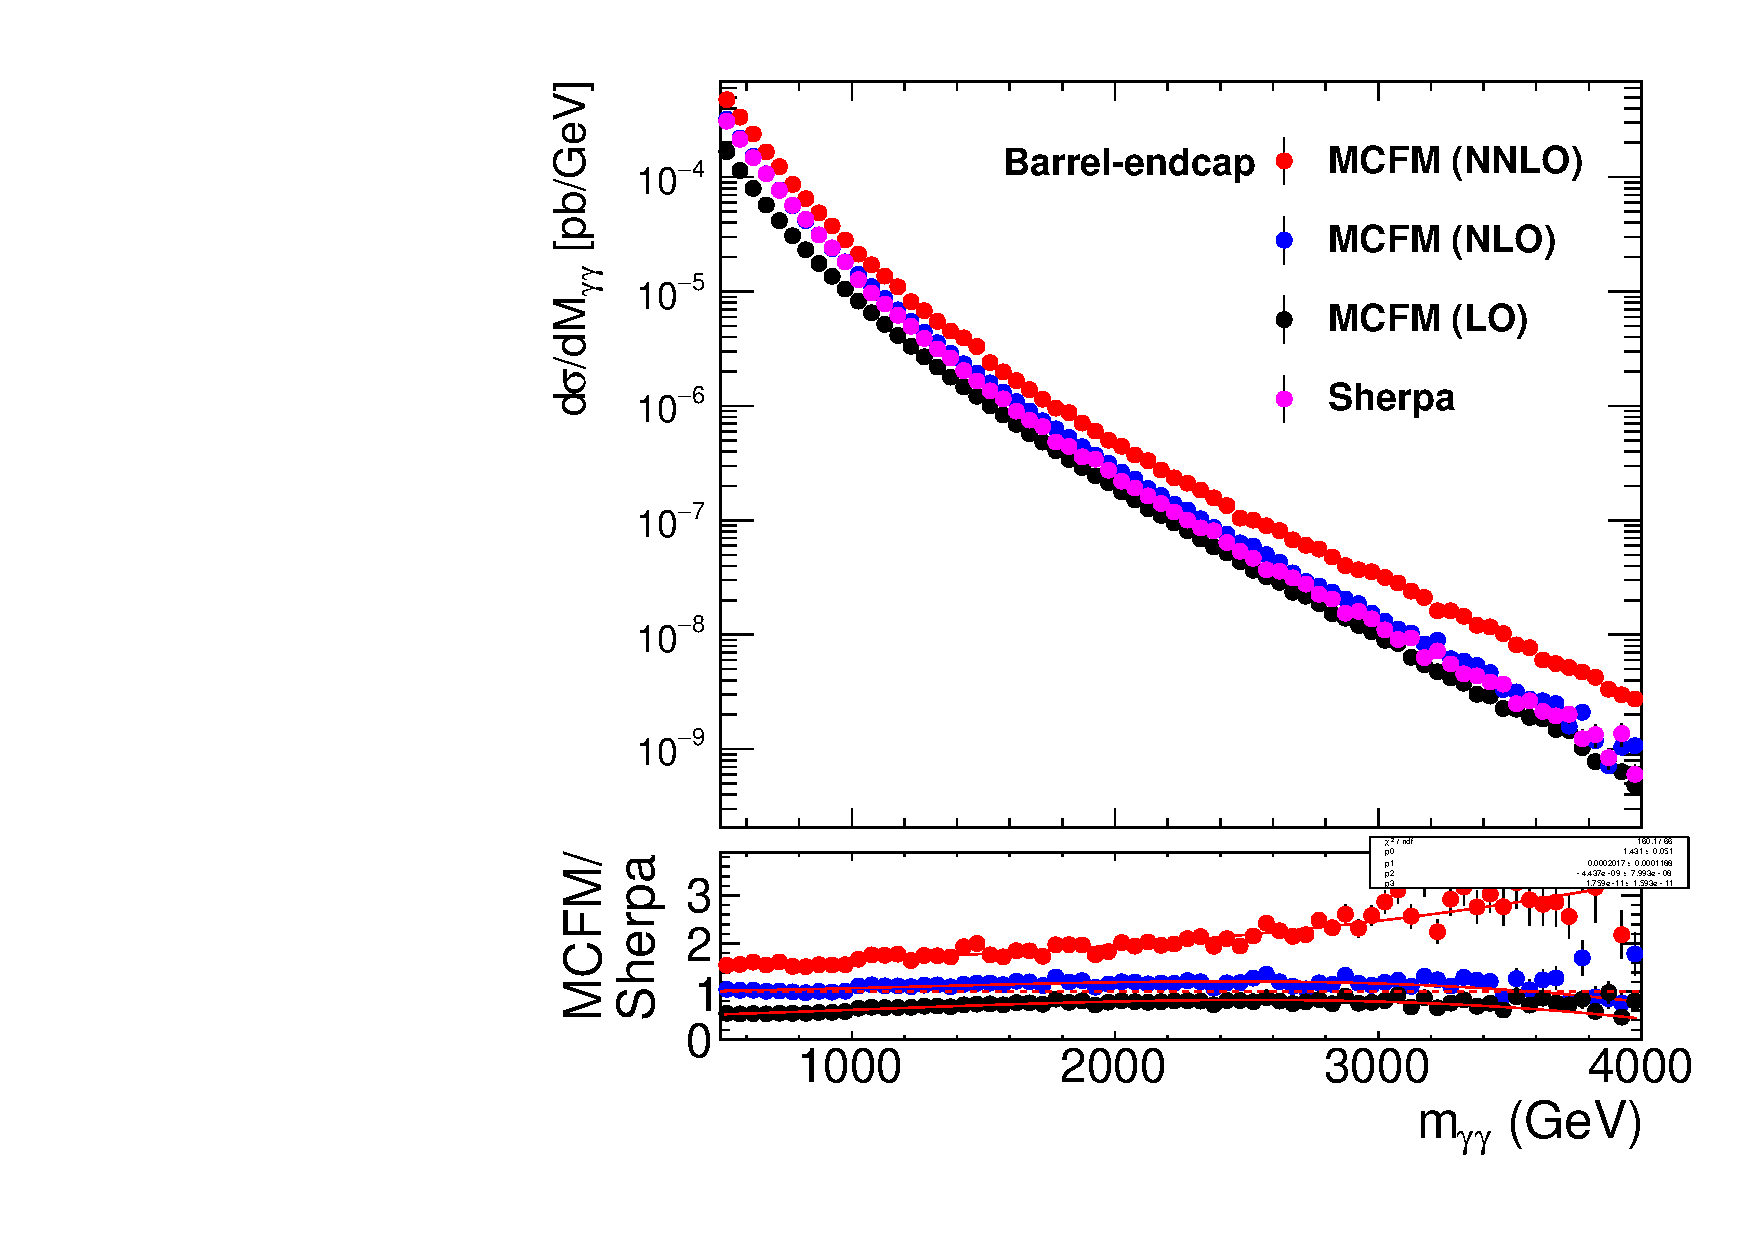
\includegraphics[angle=0,width=0.40\textwidth]{figures/BE_hist1_R1F1.pdf}
  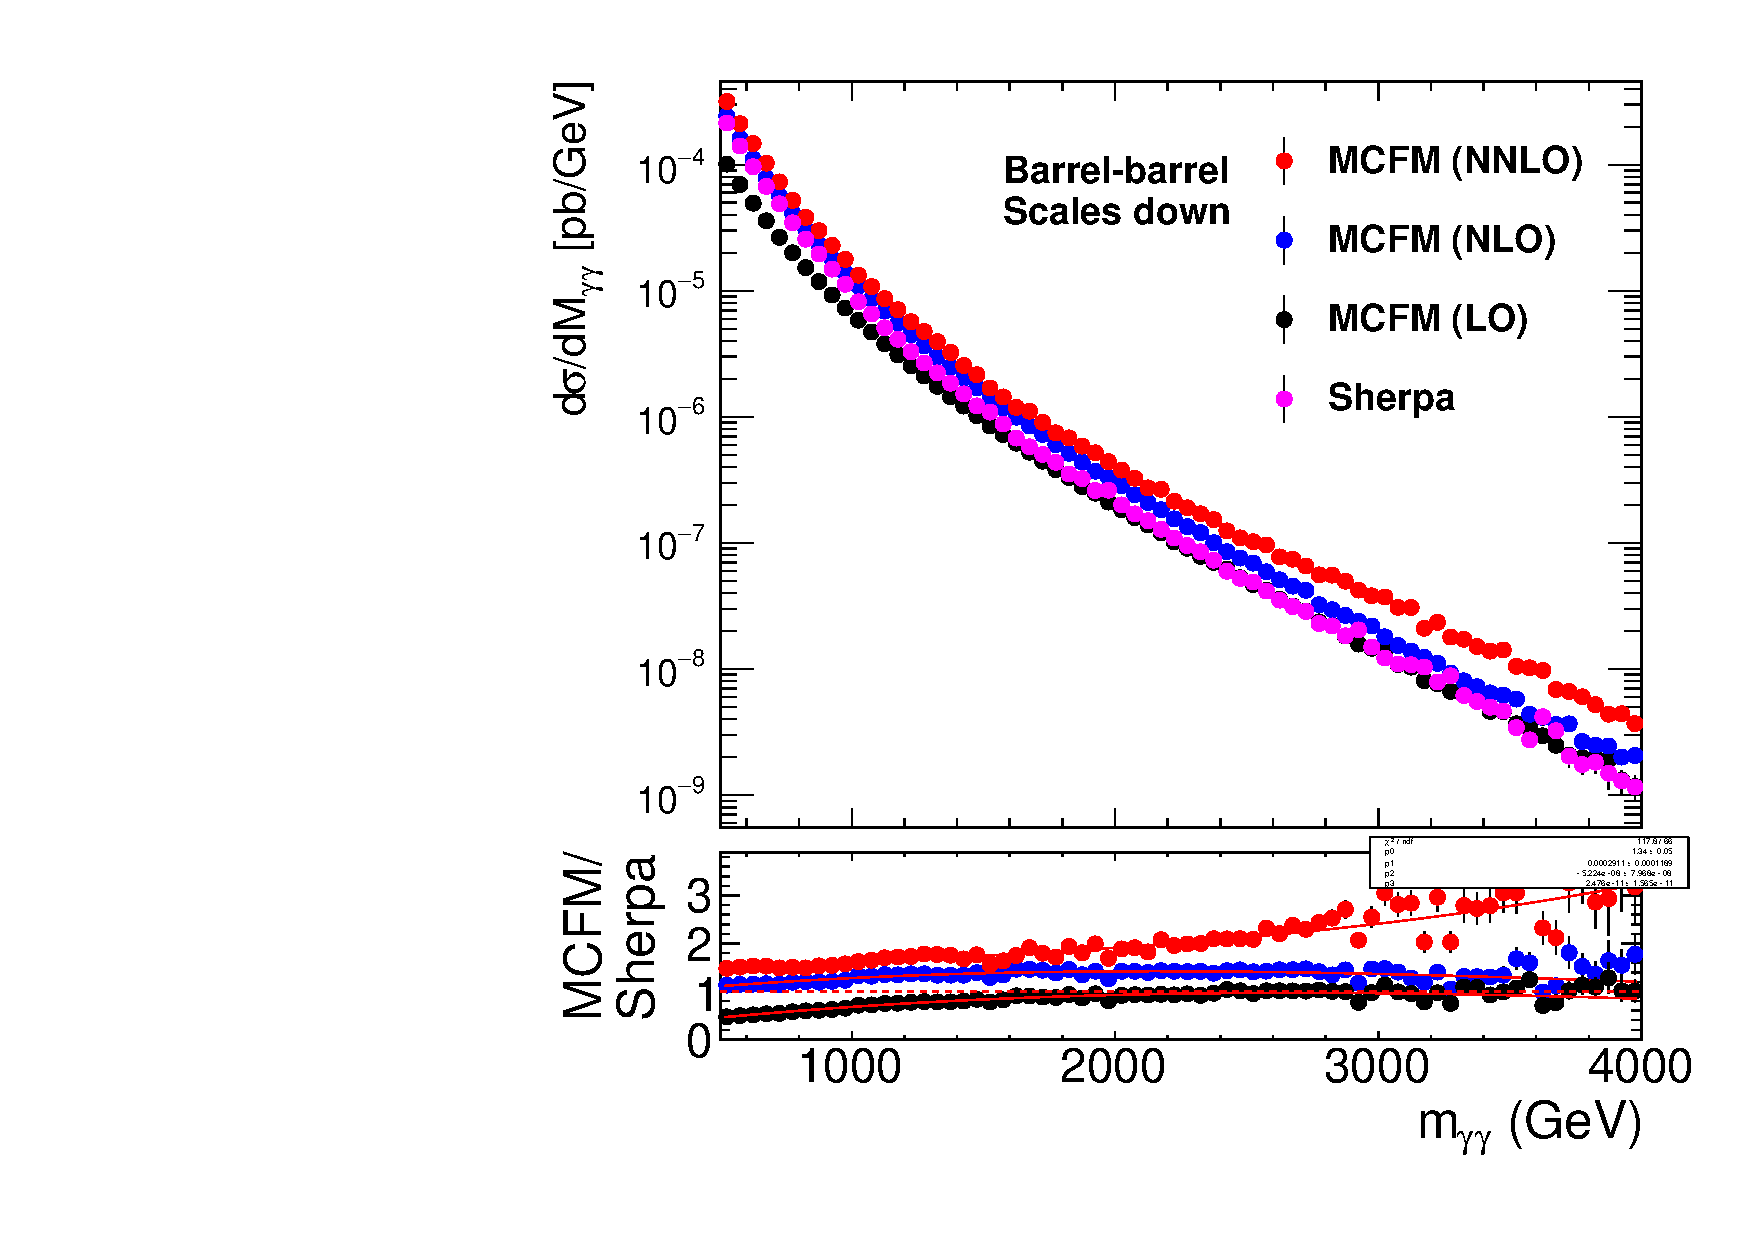
\includegraphics[angle=0,width=0.40\textwidth]{figures/BB_hist1_R0p5F0p5.pdf}
  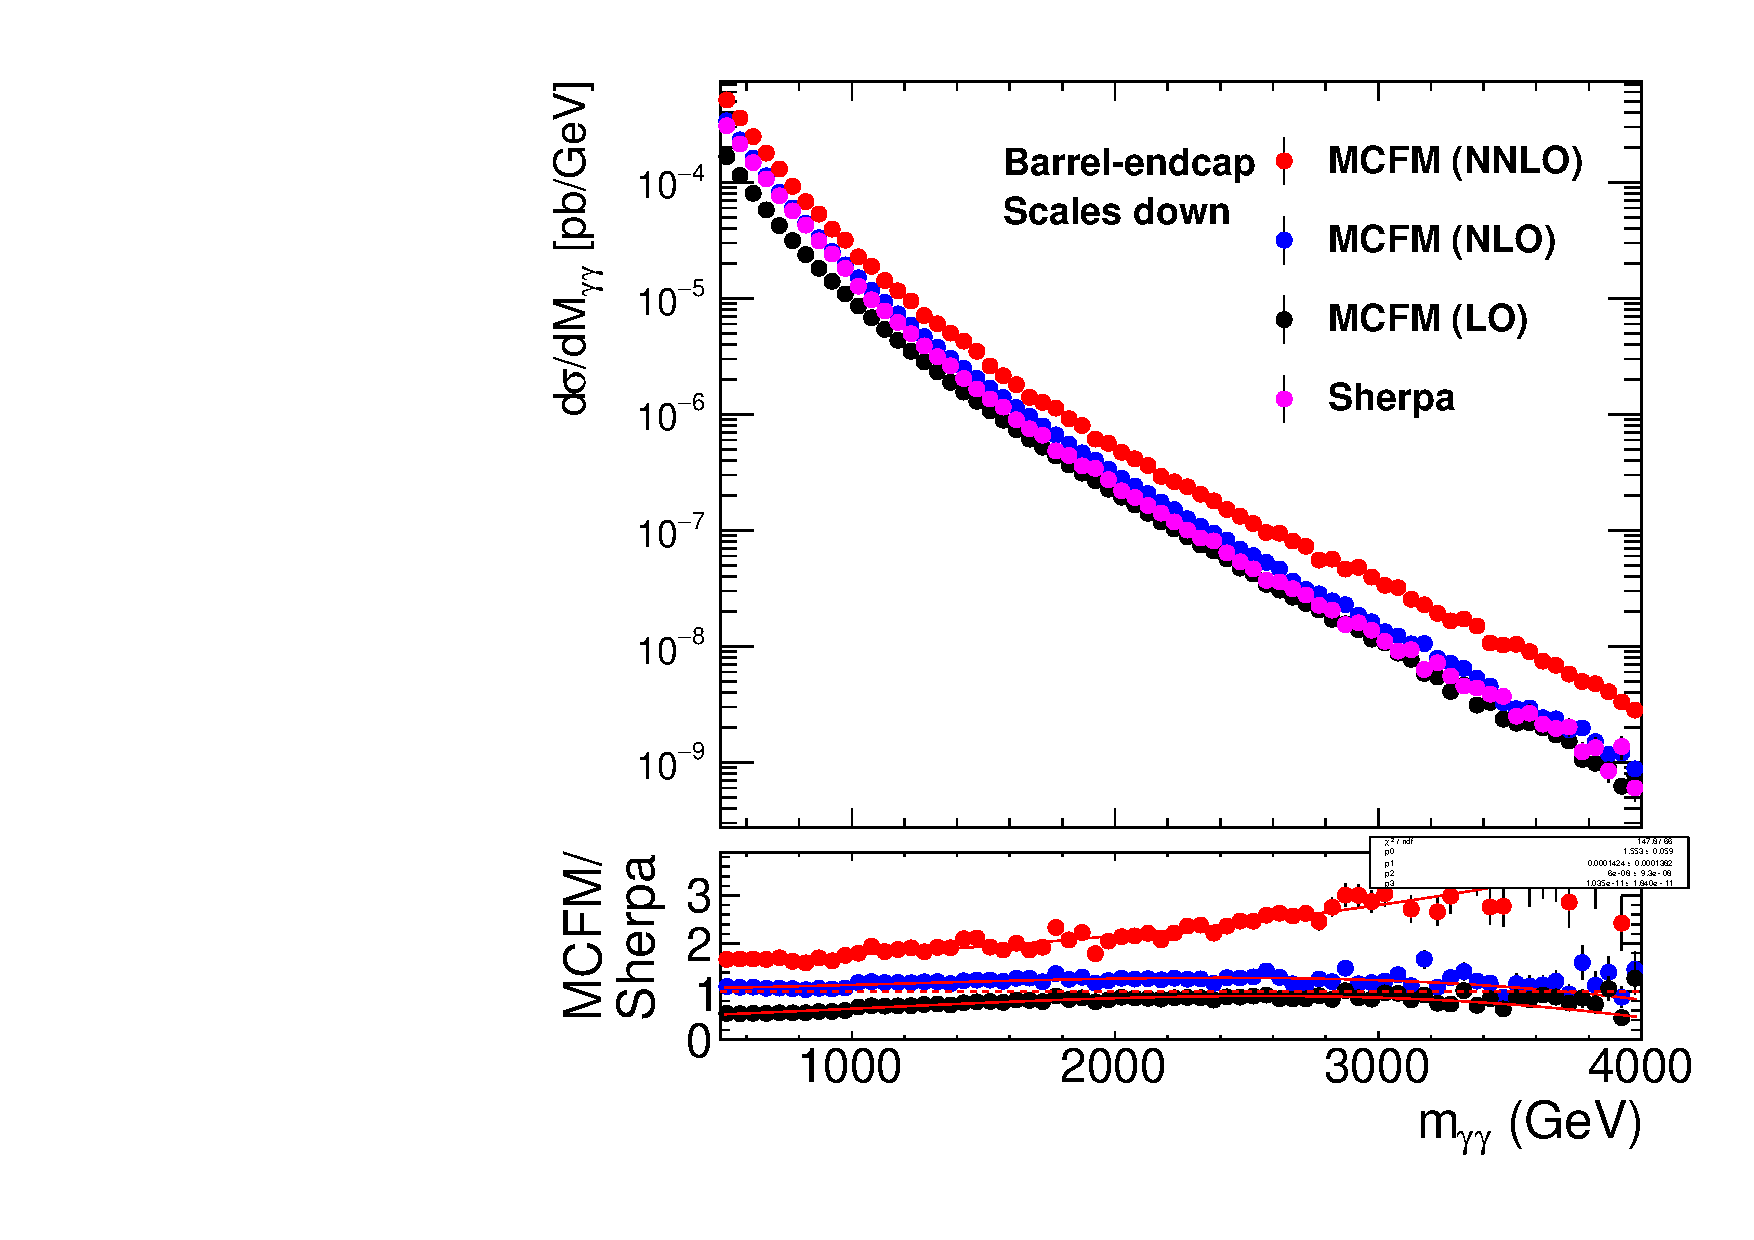
\includegraphics[angle=0,width=0.40\textwidth]{figures/BE_hist1_R0p5F0p5.pdf}
  \caption{The NNLO \Kfactor as a function of \Mgg in the EBEB (left) and EBEE (right) categories. The renormalization and factorization scales have been set to \mgg (middle) and simultaneously varied by factors of 2.0 (upper) and 0.5 (lower).}
  \label{fig:kfactor_mgg}
\end{figure}

\correction{Fig.~\ref{fig:kfactor_mgg} also shows the effects of simultaneously varying the renormalization $\mu_r$ and factorization $\mu_f$ scales by a factor of two up (upper) and down (lower) around the nominal prediction (center). The standard convention is to set these scales equal to each other and simultaneously vary them according to:}
\begin{itemize}
  \item $\mu_r = \mu_f = 2.0\Mgg$;
  \item $\mu_r = \mu_f = 1.0\Mgg$; and
  \item $\mu_r = \mu_f = 0.5\Mgg$.
\end{itemize}
\correction{\noindent These separate variations in the EBEB region are summarized for each order in Fig.~\ref{fig:kfactor_comparison_all}, which shows an envelope around the nominal \Kfactor prediction with these scales set to $1.0\Mgg$. This effect is treated as a systematic uncertainty on the analysis and is discussed in Chapter~\ref{ch:systematics}. Note, by default in \MCFM, the fragmentation scale is set to the renormalization scale. The fragmentation scale is the scale of the fragmentation functions, which describe the probability for a parton to fragment into a hadron. The variation of the renormalization scale indirectly varies this scale as well; however, its contribution is negligible when using Frixione isolation.}

\begin{figure}[htbp!]
  \centering
  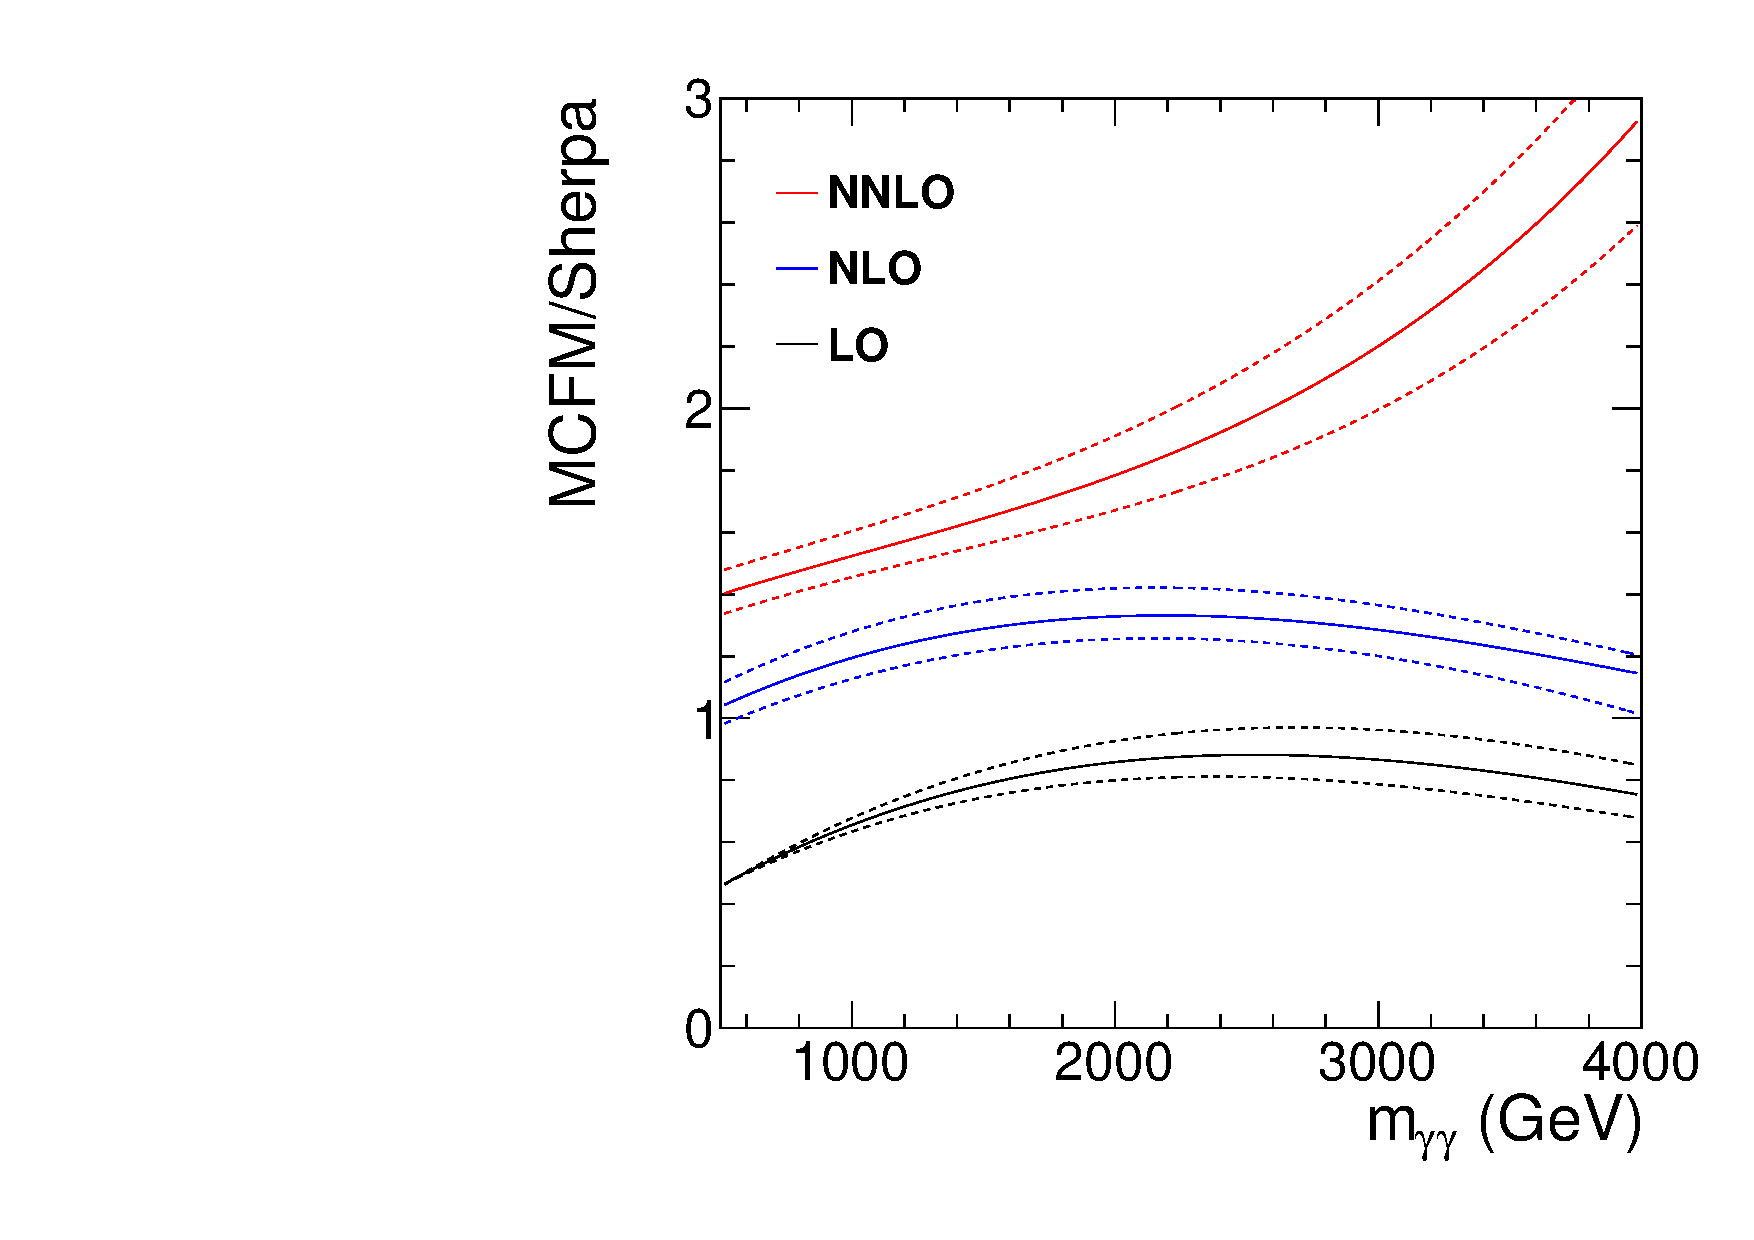
\includegraphics[angle=0,width=0.65\textwidth]{figures/kfactor_comparison.pdf}
  \caption{Ratio of the diphoton cross section calculated by \MCFM to that obtained from \SHERPA. The curves indicate different orders of the \MCFM calculation, and the dashed lines show the effect of the scale variations.}
  \label{fig:kfactor_comparison_all}
\end{figure}

\correction{The final prediction for the real SM diphoton background is determined by applying the \Kfactor to the fully simulated \SHERPA samples to reweight its events. The \Kfactor distributions are parameterized as a function of \Mgg, separately for the EBEB and EBEE categories, using a third degree polynomial function $f$ of the form}
\begin{equation}
  f(\Mgg) = p_0 + p_1\Mgg + p_2 \Mgg^2 + p_3 \Mgg^3
\end{equation}
\correction{\noindent where $p_i$, for $i=0$, 1, 2, and 3, are free parameters determined by a best fit to each distribution. The values of $p_i$ are shown in Table~\ref{tab:kfactor_values}, separately for each region. These functions are applied to the simulation-level \SHERPA events, yielding a full NNLO prediction of the real SM diphoton background.}

\begin{table}[hbt!]
  \caption{Parameters of the \Kfactor function for the EBEB and EBEE categories.}
  \label{tab:kfactor_values}
  \centering
  \vspace{\baselineskip}
  \begin{tabular}{r|rr}
    \hline
    \hline
          & EBEB & EBEE \\
    \hline
    $p_0$ & \correction{$1.25\pm0.04$} & \correction{$1.43\pm0.05$} \\
    $p_1$ & \correction{$3.36\mathrm{e}{\text{-}04}\pm1.05\mathrm{e}{\text{-}04}$} & \correction{$2.02\mathrm{e}{\text{-}04}\pm1.19\mathrm{e}{\text{-}04}$} \\
    $p_2$ & \correction{$-9.09\mathrm{e}{\text{-}08}\pm7.01\mathrm{e}{\text{-}08}$} & \correction{$-4.44\mathrm{e}{\text{-}09}\pm7.99\mathrm{e}{\text{-}08}$} \\
    $p_3$ & \correction{$2.82\mathrm{e}{\text{-}11}\pm1.38\mathrm{e}{\text{-}11}$} & \correction{$1.76\mathrm{e}{\text{-}11}\pm1.59\mathrm{e}{\text{-}11}$} \\
    \hline
    \hline
  \end{tabular}
\end{table}


\section{Background from Diphoton Misidentifications}\label{sec:fake_background}

A subdominant contribution to the total background in this search occurs when particles are misidentified as photons in the CMS detector. These particles fake a photon signature and are misreconstructed as photons. The background arising from this is referred to as the fake background. In this analysis, we consider fake photons arising from the misreconstruction of both electrons and jets. The rate for electrons faking photons is almost negligible and is readily measured from an MC calculation. To measure the rate for jets faking photons, a sophisticated technique using control samples in data is utilized.

The subdominant contribution to the fake background occurs when one or two electrons are misidentified as a photon in the detector. This mainly occurs when the electron track is misreconstructed or an electron converts late in the tracker leaving behind missing hits. This is measured using the MC simulation of Drell-Yan dielectron, $W\gamma$, $Z\gamma$, $W$, and $t\bar{t}\gamma$ events. The measurement is done by inverting the electron veto in the high-\pt photon ID and counting how many events pass this modified ID. The contribution of these fakes to the total background is calculated to be less than 1\%.

The dominant contribution to the fake background occurs when a jet with large electromagnetic activity is misidentified as a photon in the CMS detector, allowing it to pass the high-\pt photon ID criteria and, hence, fake a photon signature. The typical example of this occurs when a jet fragments to a boosted neutral meson, such as a $\pi^0$ or $\eta$, which then decays at high momentum to two photons. Both of these photons can then deposit their energy in the ECAL in such a way that their deposits overlap and resemble the signature of a single photon candidate. The fact that two photon energy deposits can become indistinguishable from one is due to the finite granularity and energy resolution of the ECAL. In a single diphoton event, this can occur from either one or two jets resulting in a photon\texttt{+}jet ($\gamma$j) or dijet (jj) background event, respectively. This type of jet fragmentation process is rare, so instead of relying on the MC simulation to accurately calculate it, a data-driven approach is preferred, which uses control samples in data to estimate to estimate the fake background contribution. The approach utilized is referred to as the fake rate method.


\subsection{Fake Rate Method}

The fake rate method involves determining a fake rate $f$ from a jet-enriched data control sample and applying it to the analysis dataset containing diphotons passing the final analysis selection. The fake rate is defined as the ratio of the number of jets passing two categories of jet fragmentation processes. The first category, the numerator of the ratio, is the number of jets passing the high-\pt photon ID. The second category, the denominator of the ratio, is the number of jets passing a looser, photon-like ID. The denominator ID is chosen such that the two categories are orthogonal. In equation form, the fake rate is
\begin{equation}
  f = \frac{(\text{numerator})}{(\text{denominator})} = \frac{\# \left\lbrace\text{jets passing the photon ID}\right\rbrace}{\# \left\lbrace\text{jets passing a photon-like ID}\right\rbrace}
\end{equation}
\noindent where \# is used to denote the number of objects in that category. This fake rate $f$ is simply the ratio of its defined categories and is not the probability that a generic jet will fake a photon.

A complication arises when determining the numerator. Although the control data sample is jet enriched, there will inevitability be a contribution to the numerator from genuine photons in it passing the photon ID, which must be removed. This is done through a fitting procedure where template models of real and fake photons are fit to the data in the control sample. These templates are constructed using a photon ID variable that is sensitive to the differences between real and fake photons, such as a shower shape or isolation variable. After the fit is performed, the contribution to the numerator from real photons will be subtracted from the total. In general, the choice of template variable will evolve with photon \pt and $\eta$. Therefore, the fake rate $f$ will be measured as a function of photon \pt and categorized in the EB and EE regions.

After the final fake rate function $f(\pt)$ is determined separately in the EB and EE categories (from the data control sample), it will then be applied to the final, analysis-level diphoton dataset. This is done by selecting objects in the diphoton dataset that pass the denominator, photon-like ID and reweighting them using $f(\pt)$, separately in the EBEB and EBEE categories. The assumption in doing this final step is that taking denominator objects and reweighting them by the fake rate does indeed produce an accurate representation of the kinematics of known fake events. Physically, we expect this to be true because jet fragmentation is largely independent of the rest of the event. \correction{Thus, events where a jet fragments to look like a denominator, photon-like jet should be representative of other events where the jet fragmented differently and ended up faking the photon ID, since we want to measure the number of jets passing the photon ID by using jets that pass the denominator ID.} Verification of the ability of the fake rate method to achieve this is demonstrated in simulation and is described in Section~\ref{sec:closure_test_kinematics}.

\correction{To validate the fake rate method, a closure test is performed on a sample of simulated data produced from an MC calculation.} The idea is to apply the fake rate method to the simulated sample in the identical way as it is done in the jet-enriched control dataset. This yields a fake prediction in the simulated sample. Now, because we are using simulation, we have access to the MC truth information for the particles, i.e., we know the properties and full event history of all the particles in the simulated sample. In particular, we know the identities of all of the particles in it passing the high-\pt photon ID. Therefore, using the truth information, we can tag objects passing the photon ID as having arisen from jets or from real, prompt photons. Finally, we can compare these fake yields to the fake prediction in the simulated sample. In addition, we also perform further studies to validate the method, as will be explored in Section~\ref{ssec:closure_test}.


\subsection{Fake Rate Calculation}

The data control sample used for the photon fake rate calculation comes from a combination of jet- and muon-triggered data samples. The list of samples using the full, internal CMS dataset path names are tabulated in Table~\ref{tab:fake_rate_datasets}. This combination of datasets has been constructed to help eliminate any potential bias arising from the differences in the hadronization between quarks and gluons. In general, gluon jets contain a higher number of particles, as discussed in Section~\ref{sec:jets}, and are therefore less likely to pass the isolation variables in the photon ID, so they should have a lower probability of faking a photon than a quark jet. It is difficult to distinguish between quark and gluon jets in data, but these datasets result from different processes and will help better sample jet flavor in the control sample.

\begin{table}[!htbp]
  \caption{Control datasets used for the photon fake rate calculation.}
  \label{tab:fake_rate_datasets}
  \centering
  \vspace{\baselineskip}
  \small %\normalsize %\footnotesize
  \begin{tabular}{l}
  \hline
  \hline
  Dataset path \\
  \hline
  /JetHT/Run2016B-23Sep2016-v3/MINIAOD \\
  /JetHT/Run2016C-23Sep2016-v1/MINIAOD \\
  /JetHT/Run2016D-23Sep2016-v1/MINIAOD \\
  /JetHT/Run2016E-23Sep2016-v1/MINIAOD \\
  /JetHT/Run2016F-23Sep2016-v1/MINIAOD \\
  /JetHT/Run2016G-23Sep2016-v1/MINIAOD \\
  /JetHT/Run2016H-PromptReco-v2/MINIAOD \\
  /JetHT/Run2016H-PromptReco-v3/MINIAOD \\
  \hline
  /DoubleMuon/Run2016B-23Sep2016-v3/MINIAOD \\
  /DoubleMuon/Run2016C-23Sep2016-v1/MINIAOD \\
  /DoubleMuon/Run2016D-23Sep2016-v1/MINIAOD \\
  /DoubleMuon/Run2016E-23Sep2016-v1/MINIAOD \\
  /DoubleMuon/Run2016F-23Sep2016-v1/MINIAOD \\
  /DoubleMuon/Run2016G-23Sep2016-v1/MINIAOD \\
  /DoubleMuon/Run2016H-PromptReco-v2/MINIAOD \\
  /DoubleMuon/Run2016H-PromptReco-v3/MINIAOD \\
  \hline
  \hline
  \end{tabular}
\end{table}

As the proton beams circulate, they may interact with the LHC collimators or residual gas in the beam pipe due to the non-perfect vacuum, creating ``beam halo." When the protons interact with the particles associated with these sources, jets will be formed and can subsequently fragment to other high-energy particles, which are not produced from the collision point of the bunch crossing. This will produce charged pions ($\pi^{\pm}$), which will travel an average distance of about 10~m before decaying, primarily to muons ($\mu^{\pm}$). These muons will travel parallel to the beam pipe and can traverse the whole detector, producing high-energy bremsstrahlung photons in the ECAL. Beam halo could fake a photon signature and must be eliminated in the fake rate measurement. This \correction{source can be identified and rejected} by using the photon shower shape variables \sieie and \sipip. Beam halo will be well contained in the $\phi$ direction but spread out in the $\eta$ direction as it interacts with the CMS detector. This is in contrast to prompt photons, which are well contained in the $\eta$ direction. Fig.~\ref{fig:sipip_vs_sieie} shows the correlation between \sieie and \sipip for all objects in the jet-triggered dataset passing the high-\pt photon ID (with the \sieie cut relaxed) in the range $450<\pt<500\GeV$. In this high-energy range, cutting at $\sipip > 0.009$ will safely reject the beam halo.

\begin{figure}[!htbp]
  \centering
  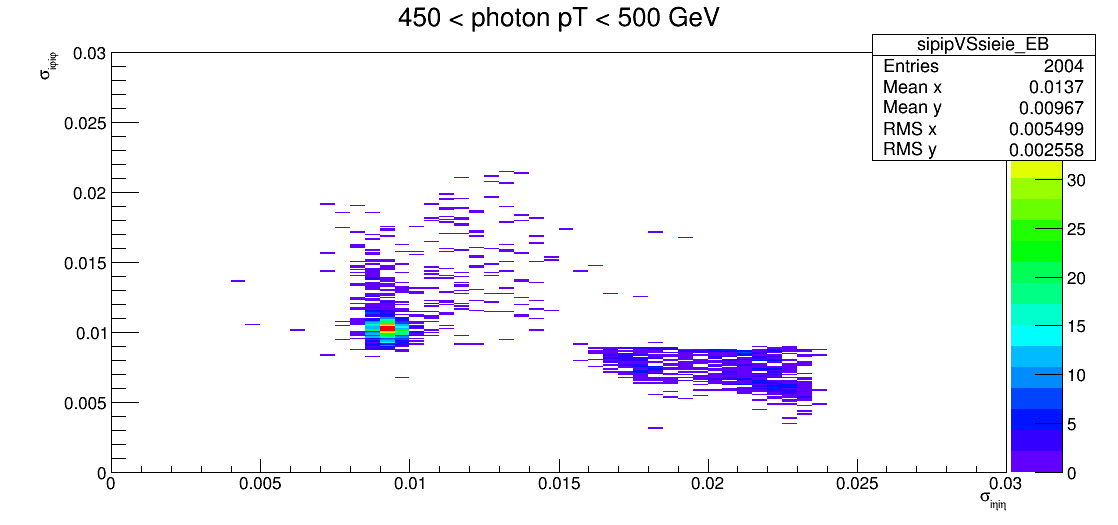
\includegraphics[scale=0.43]{figures/sipip_vs_sieie_EB_pT450-500.png}
  \caption{The correlation between \sieie and \sipip for all objects in the jet-triggered control dataset (used for the fake rate calculation) passing the high-\pt photon ID (with the \sieie cut relaxed) in the range $450<\pt<500\GeV$. Beam halo is observed for $\sipip < 0.009$.}
  \label{fig:sipip_vs_sieie}
\end{figure}

The denominator objects are chosen to pass a less strict version of the high-\pt photon ID. These photon-like jets should have high electromagnetic energy content but are required to fail at least one of the photon ID variables, ensuring the denominator category is orthogonal to the numerator category, as well as eliminating any contamination from real photons. We want these objects to be representative of the kinematics of the reweighted events in the diphoton data sample. They should be reasonably isolated since not all of the energy of the particles in a cone of $\Delta R$ around the object is added to it, while, on the other hand, \correction{we need to ensure there is enough statistics} after loosening the isolation criteria. Different cuts are imposed in the EB and EE regions to optimize the selection in each category. Denominator objects in the EB are required to fail at least one of the variables \hoe, \sieie, \chiso, or \corphoiso. In addition, they are required to pass both $\chiso < 0.2\,\pt$ and $\corphoiso < 0.2\,\pt$. Because of pileup mismodeling in the $\phoiso$ variable during the 2016 data-taking period, denominator objects in the EE category are required to pass the photon ID cut of $\corphoiso < 2.0\GeV$, instead of the looser selection of $\corphoiso < 0.2\,\pt$. In the EE regions, the denominator objects are also required to pass $\chiso < 0.2\,\pt$ and fail at least one of the variables \hoe, \sieie, or \chiso. These cuts will be summarized in Table~\ref{tab:fake_rate_cuts} below after some further discussion.

An additional cut for denominator objects on the ratio the hadronic over electromagnetic energies using $\text{Hadronic/E}$ is imposed in both the EB and EE regions. As discussed in Section~\ref{sec:trigger}, the variable \hoe using a tower-based isolation to sum the hadronic energy deposits while $\text{Hadronic/E}$ uses a cone-based calculation. The trigger selection used in the analysis (\texttt{HLT\_DoublePhoton60}) requires $\text{Hadronic/E}$ at the HLT level and is not fully efficient for denominator objects, even for those passing $\hoe < 0.05$, while it is for objects passing the high-\pt photon ID. This is remedied by applying an additional cut of $\text{Hadronic/E} < 0.1$ to the denominator objects.

The numerator objects result from the selection of objects in the jet-enriched dataset passing the high-\pt photon ID and adjusted so that any contamination from real photons is removed through a template fitting procedure. The template variable used is the shower shape variable \sieie. The data to be fit to are the numerator candidates in the jet-enriched dataset consisting of all objects passing the high-\pt photon ID with \sieie relaxed, to be summarized in Table~\ref{tab:fake_rate_cuts} below. Since \sieie evolves with photon \pt, the data are divided into the nine photon \pt bins of 50-70, 70-90, 90-110, 110-130, 130-150, 150-200, 200-250, 250-300, and 300-600\GeV. (The denominator objects are also split into these bins resulting in a fake rate for each bin.) The numerator candidates in each \pt bin are split into their real and fake components using templates derived from respective models of real and fake photons.

The fake templates are derived from the jet-enriched dataset. Since real photons are well isolated after pileup subtraction, in particular, the high-\pt photon ID requires $\chiso < 5\GeV$, fake photons can be modeled by inverting this isolation requirement. Objects in the fake templates must pass the high-\pt photon ID with \sieie relaxed but are taken from the sideband of $5 < \chiso < 10\GeV$. Notice, we are trying to describe fake photons with $\chiso < 5\GeV$ by modeling them from the selection using $5 < \chiso < 10\GeV$. The evolution of the fake templates with \pt from the jet-triggered dataset is shown in Fig.~\ref{fig:fake_templates}. These templates are scaled to 1\fbinv and shown separately in the EB and EE regions.

\begin{figure}[!htbp]
  \centering
  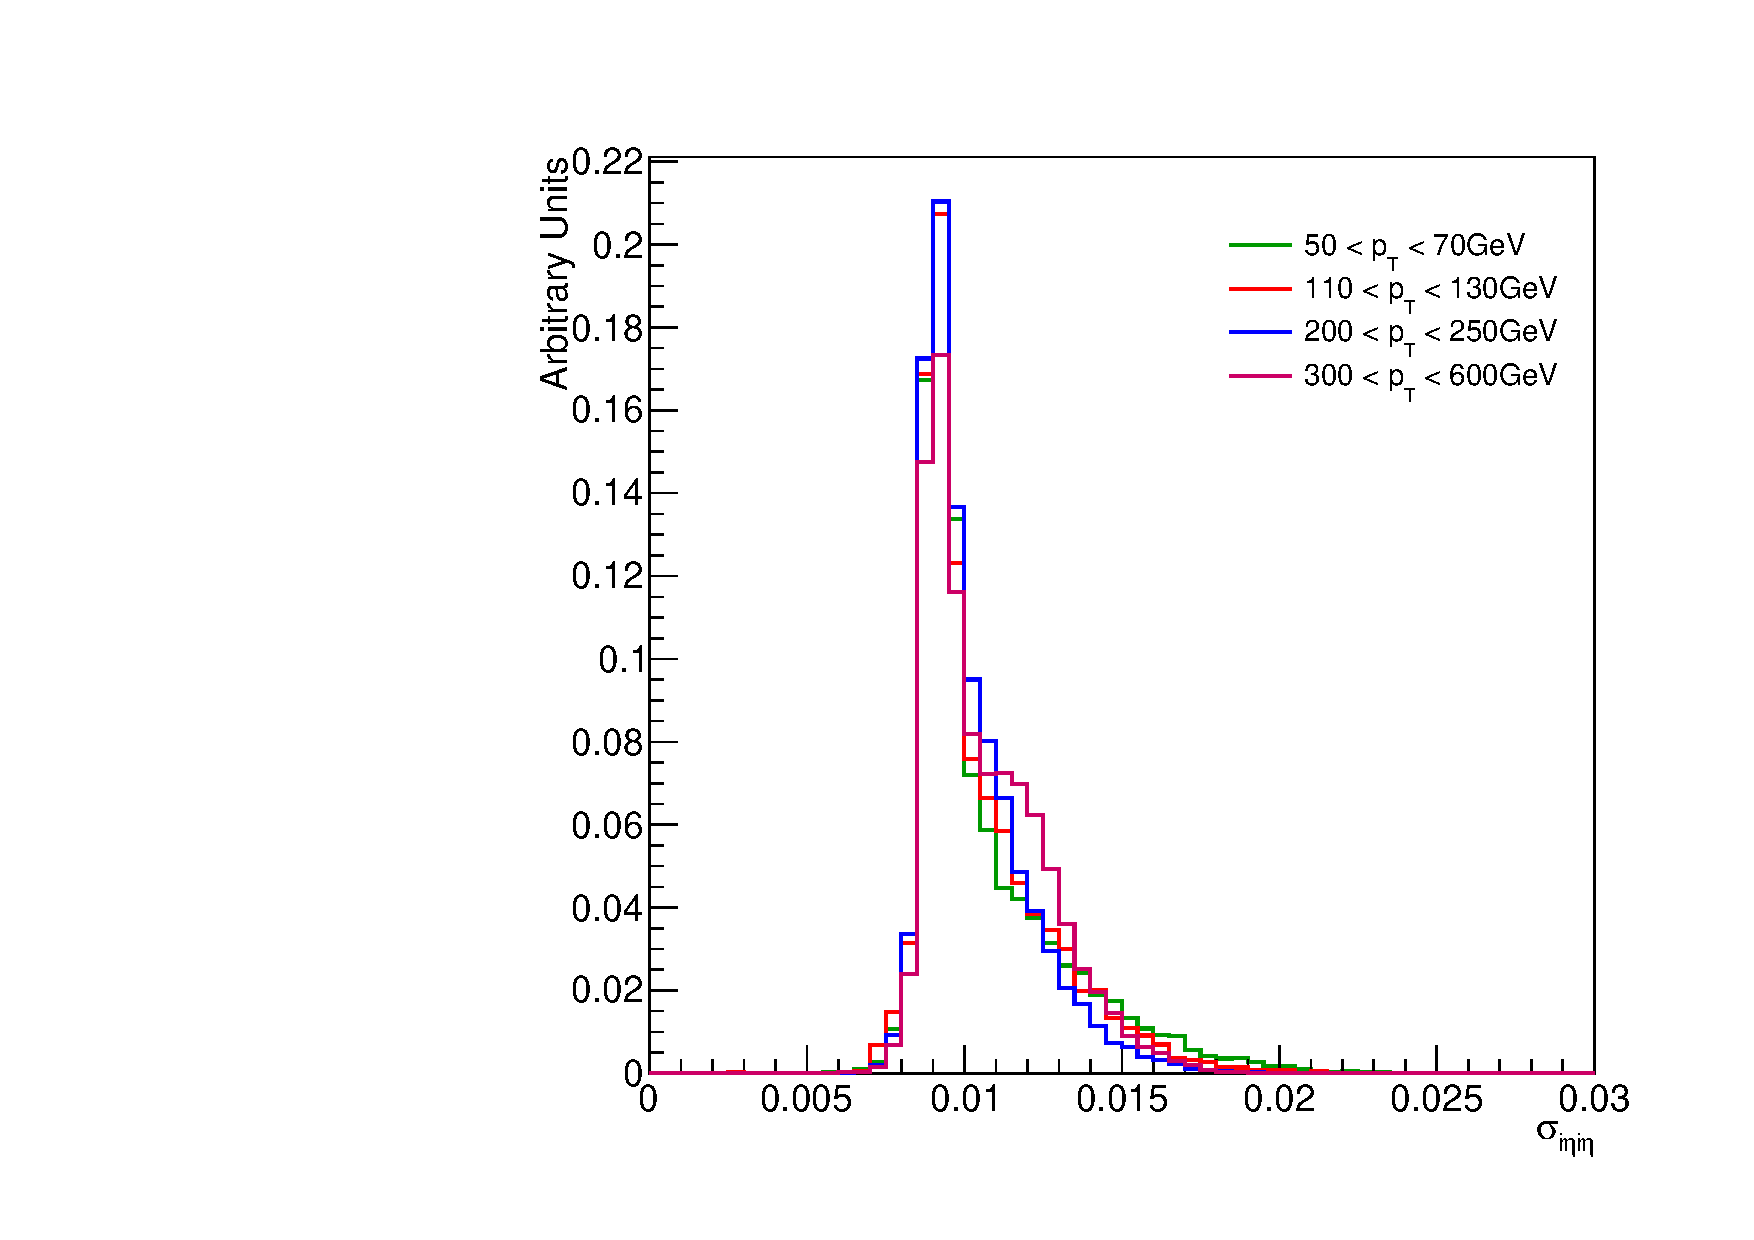
\includegraphics[width=0.45\textwidth]{figures/faketemplatecompEB.pdf}
  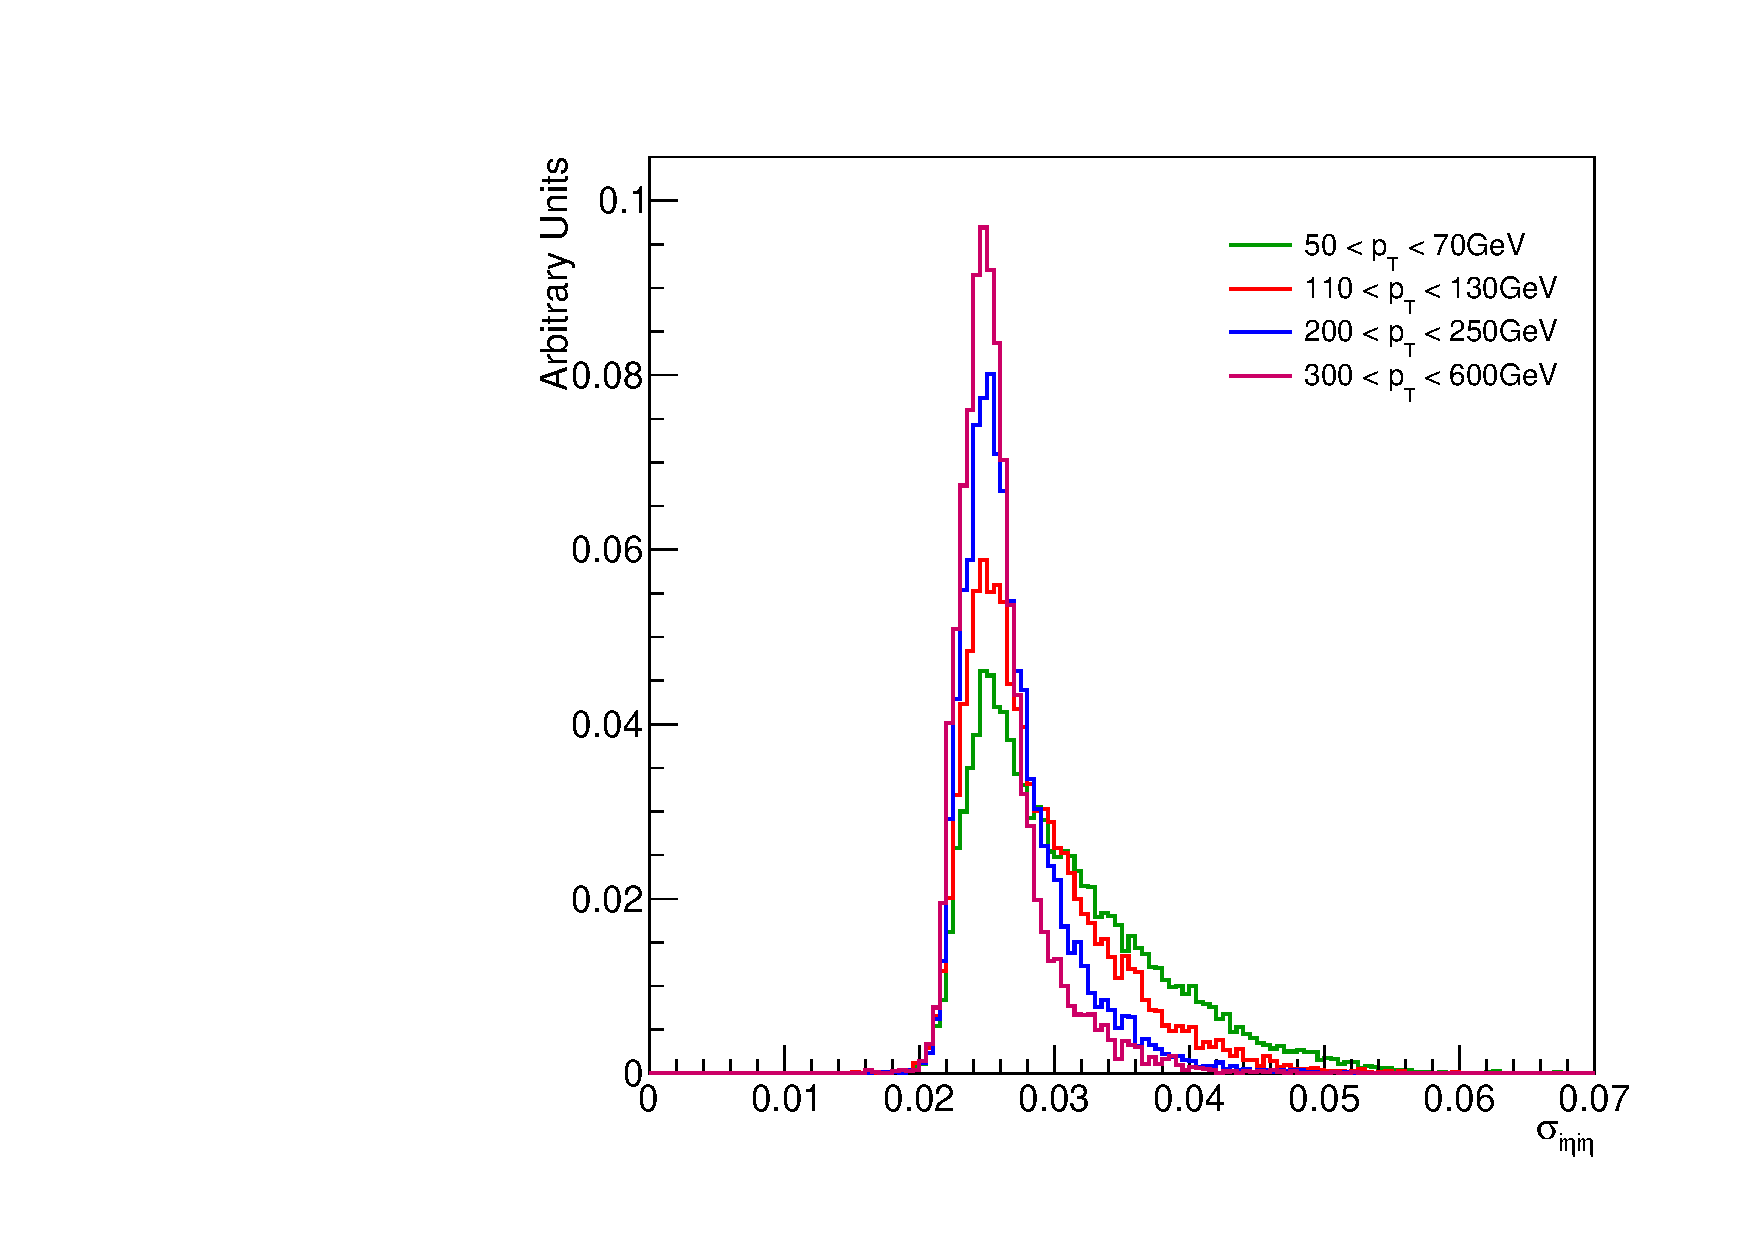
\includegraphics[width=0.45\textwidth]{figures/faketemplatecompEE.pdf}
  \caption{Fake templates scaled to 1\fbinv in various \pt bins in the EB (left) and EE (right) regions.}
  \label{fig:fake_templates}
\end{figure}

The real templates are derived from a photon-rich simulated sample produced using an MC calculation. The $\gamma\gamma$ MC background samples, listed in Table~\ref{tab:ggjets_samples}, are used for this. In addition, the $\gamma$j MC samples produced centrally within the CMS Collaboration are added to allow for a source of prompt photons coming from processes using the $\gamma$j final state. The full list of samples is given in Table~\ref{tab:real_template_samples}. Within the photon-rich MC sample, all objects passing the high-\pt photon ID with relaxed \sieie are selected, but only those coming from known prompt photons are allowed in the real templates. The definitions for both the real and fake templates are summarized in Table~\ref{tab:fake_rate_cuts}. It's possible to identify these real photons since the MC truth information is provided for all generated particles.

\begin{table}[!htbp]
  \caption{The MC samples and corresponding cross sections used for deriving the real templates in the fake rate calculation. The full, internal CMS path name is specified by appending the dataset path with \texttt{/RunIISummer16MiniAODv2-\allowbreak PUMoriond17\_\allowbreak 80X\_\allowbreak mcRun2\_\allowbreak asymptotic\_\allowbreak 2016\_\allowbreak TrancheIV\_\allowbreak v6/\allowbreak MINIAODSIM}.}
  \label{tab:real_template_samples}
  \centering
  \vspace{\baselineskip}
  %\footnotesize
  \small
  \begin{tabular}{lc}
  \hline
  \hline
  Dataset path & Cross section (pb) \\ 
  \hline
  /GGJets\_M-60To200\_Pt-50\_13TeV-sherpa & 5.785 \\
  /GGJets\_M-200To500\_Pt-50\_13TeV-sherpa & 2.244 \\
  /GGJets\_M-500To1000\_Pt-50\_13TeV-sherpa & 1.510 \\
  /GGJets\_M-1000To2000\_Pt-50\_13TeV-sherpa & 1.084e-02 \\
  /GGJets\_M-2000To4000\_Pt-50\_13TeV-sherpa & 3.690e-04 \\
  /GGJets\_M-4000To6000\_Pt-50\_13TeV-sherpa & 2.451e-06 \\
  /GGJets\_M-6000To8000\_Pt-50\_13TeV-sherpa & 1.753e-08 \\
  /GGJets\_M-8000To13000\_Pt-50\_13TeV-sherpa & 7.053e-11 \\
  \hline
  /GJets\_HT-40To100\_TuneCUETP8M1\_13TeV-madgraphMLM-pythia8 & 2.121e+04 \\
  /GJets\_HT-100To200\_TuneCUETP8M1\_13TeV-madgraphMLM-pythia8 & 9.863e+03 \\
  /GJets\_HT-200To400\_TuneCUETP8M1\_13TeV-madgraphMLM-pythia8 & 2.298e+03 \\
  /GJets\_HT-400To600\_TuneCUETP8M1\_13TeV-madgraphMLM-pythia8 & 2.816e+02 \\ 
  /GJets\_HT-600ToInf\_TuneCUETP8M1\_13TeV-madgraphMLM-pythia8 & 9.465e+01 \\
  \hline \hline
  \end{tabular}
\end{table}

\begin{table}[!htbp]
  \caption{The cut-based definitions of the numerator and denominator objects for the fake rate calculation compared against the high-\pt photon ID. The numerator is determined after numerator candidates are fit with real and fake templates (definitions shown) using the template variable \sieie. The cuts listed are for both the EB and EE regions unless separately specified.}
  \label{tab:fake_rate_cuts}
  \centering
  \vspace{\baselineskip}
  \tiny
  \begin{tabular}{l|cccccc}
  \hline \hline
  Cut [EB \{sat.\} (EE \{sat.\})] & Photon ID & Num. & Real template & Fake template & Denom. (EB) & Denom. (EE) \\
  \hline
   & & & & & & \\
  \textbf{Photon ID cuts} & & & & & & \\
  \hline
  $\hoe < 0.05$ & pass & pass & pass & pass & \multirow{5}{*}{fail at least one} &  \multirow{4}{*}{fail at least one} \\
  $\sieie < 0.0105\, \{0.0112\}\, (0.028\, \{0.030\})$ & pass & template & template & template & & \\
  $\chiso < 5\GeV$ & pass & pass & pass & not applied & & \\
  $\corphoiso < 2.75\, (2.00)\GeV$ & pass & pass & pass & pass & & pass \\
  $\rnine > 0.8$ & pass & pass & pass & pass & pass & pass \\
   & & & & & & \\
  \textbf{Electron veto} & & & & & & \\
  \hline
  CSEV & pass & pass & pass & pass & pass & pass \\
   & & & & & & \\
  \textbf{Additional fake rate cuts} & & & & & & \\
  \hline
  $\sigma_{i\phi i\phi} > 0.009$ & not applied & pass & pass & pass & pass & pass \\
  $5 < \chiso < 10\GeV$ & not applied & not applied & not applied & pass & not applied & not applied \\
  $\text{Hadronic/E} < 0.1$ & not applied & not applied & not applied & not applied & pass & pass \\
  $\chiso < 0.2\,\pt$ & not applied & not applied & not applied & not applied & pass & pass \\
  $\corphoiso < 0.2\,\pt$ & not applied & not applied & not applied & not applied & pass & not applied \\
  \hline \hline
  \end{tabular}
\end{table}

The procedure used to ensure only real photons are selected is to first find the best match in $\Delta R$ among all the final state generated particles to the reconstructed photon object passing the photon ID. Next, the best match is required to be a generated photon within $\Delta R<0.1$. If the matched generated photon can be traced back to the hard interaction, then the reconstructed photon object is included in the real template. Fig.~\ref{fig:real_templates} shows the evolution of these real templates (each scaled to 1\fbinv) with photon \pt in both the EB and EE categories.

\begin{figure}[!htbp]
  \centering
  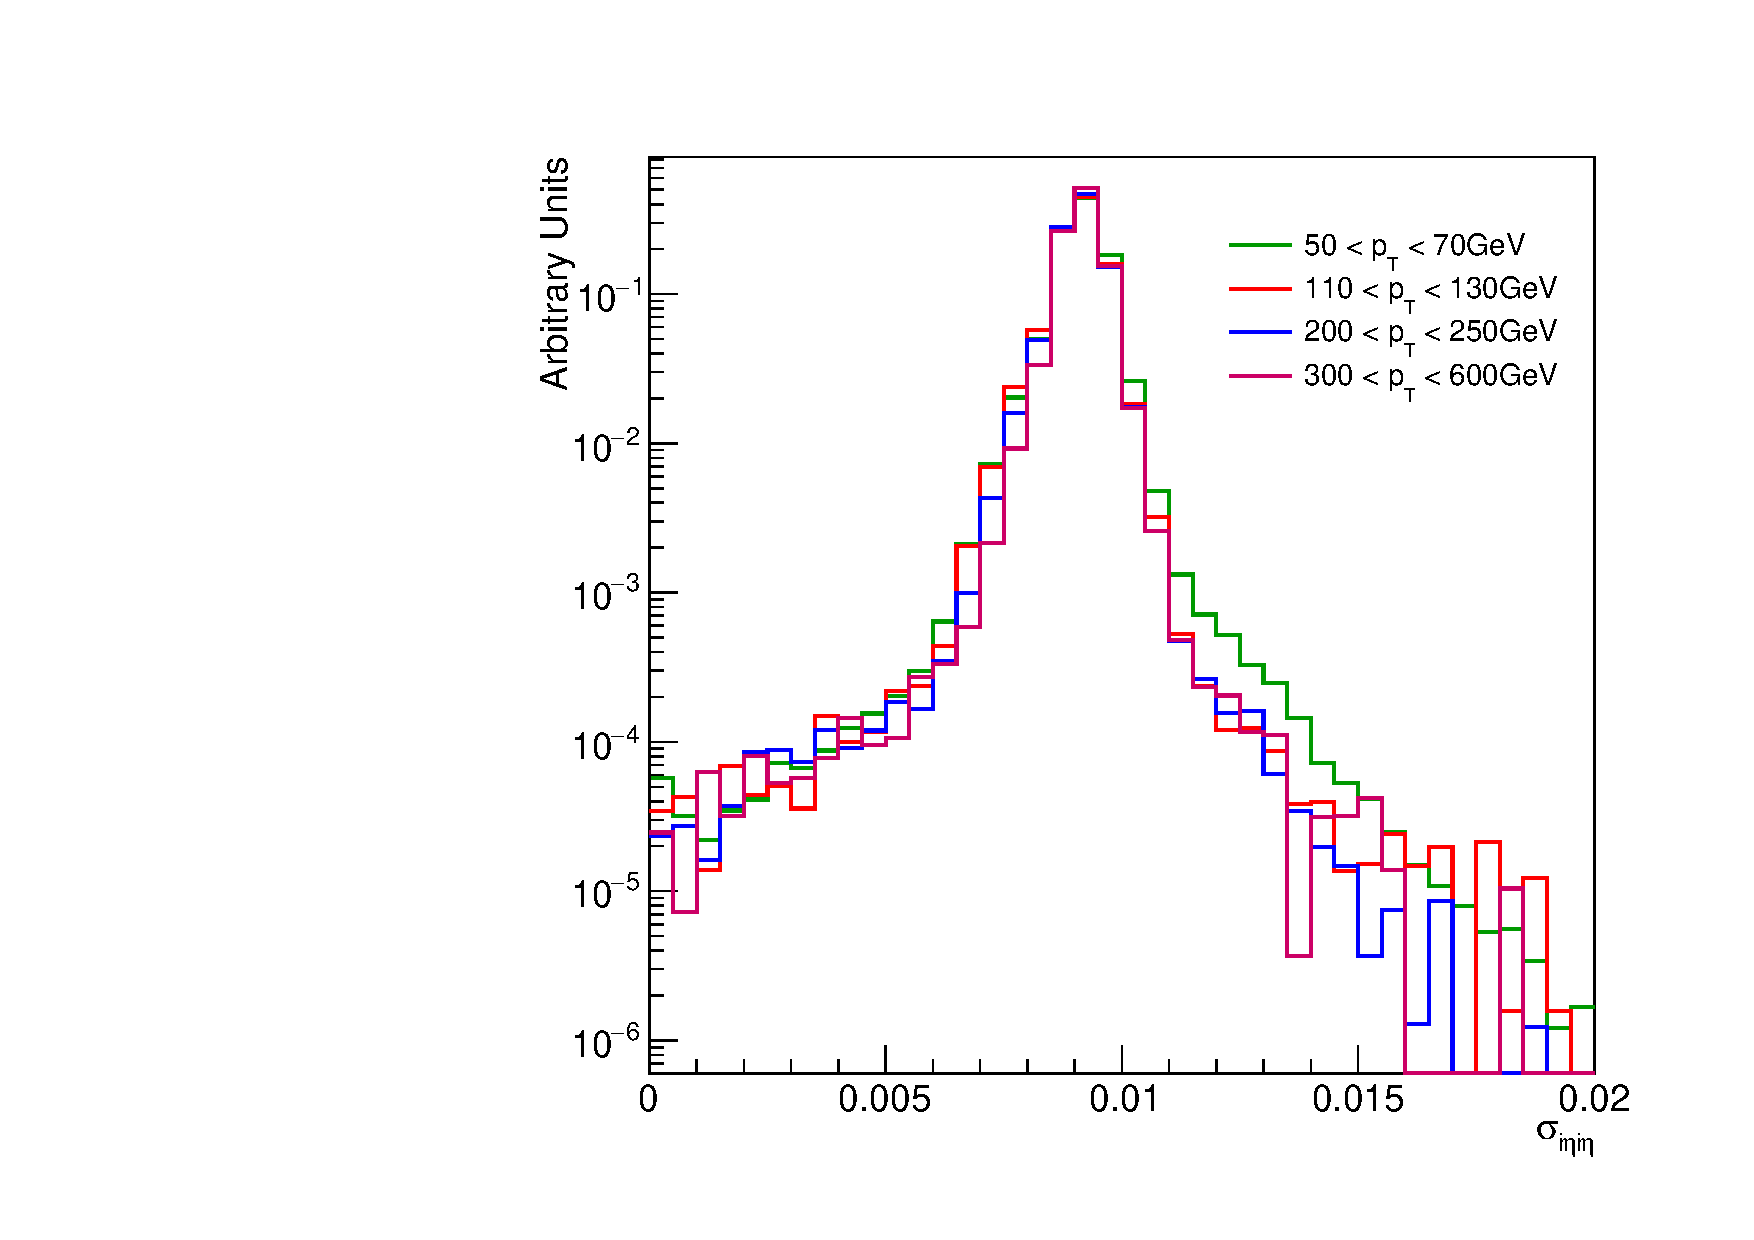
\includegraphics[width=0.45\textwidth]{figures/realtemplatecompEB.pdf}
  \includegraphics[width=0.45\textwidth]{figures/realtemplatecompEE.pdf}
  \caption{Real templates scaled to 1\fbinv in various photon \pt bins in the EB (left) and EE (right) regions.}
  \label{fig:real_templates}
\end{figure}

With the construction of the fake and real templates, they can both be fit to the numerator candidates in the control data sample. The shapes of the templates are fully determined from their construction, but their normalization is determined from the fit to the data. First the templates are normalized to $1\fbinv$, then a simultaneous fit using a maximum likelihood estimation is performed. A negative log-likelihood is used in a procedure similar to what is employed in Chapter~\ref{ch:results}. \correction{An example fit in the EB region for the 130-150\GeV \pt bin is shown in Fig.~\ref{fig:template_fit}. We see that the tail region with $\sieie > 0.011$ is dominated by fakes, which largely fixes the overall fake normalization.} The general trend showing that the real template dominates the overall normalization in the peak and the fake template in the tail holds true for the other \pt bins and also in the EE category. This final fit shows the contribution of fakes within the data. To extract the numerator, the fake template is integrated from 0 to \sieie cut value, which differs between the EB and EE categories. This process is repeated for all \pt bins in both categories.

\begin{figure}[!htbp]
  \centering
  \includegraphics[width=1.0\textwidth]{figures/fakeRatePlotEB_pT130To150_chIso5To10.pdf}
  \caption{A template fit in the EB with $130<\pt<150\GeV$, shown in linear (left) and log (right) scale.}
  \label{fig:template_fit}
\end{figure}

Dividing the numerator yields by the denominator gives the fake rates in the nine \pt bins for both the EB and EE categories, as shown in Fig.~\ref{fig:fake_rate}. These are represented by the black data points with horizontal error bars showing the bin widths. The statistical uncertainties from the denominator distributions and the template fits are represented by the vertical, black error bars. The vertical, blue error bars represent the change in the fake rates under a variation of the \chiso sideband, to be discussed in more detail below in Section~\ref{ss:fr_studies}. The larger fake rate in the EE category is caused by imposing the $\corphoiso < 2.0\GeV$ cut in the denominator selection, which is different for the EB category. The best fit to these fake rate points is shown in red, giving the final fake rate as a function of photon \pt.

\begin{figure}[!htbp]
  \centering
  \includegraphics[width=0.49\textwidth]{figures/EBfit2016.pdf}
  \includegraphics[width=0.49\textwidth]{figures/EEfit2016.pdf}
  \caption{The fake rate in different photon \pt bins for the EB (left) and EE (right) categories. The fake rate function (red) is the best fit to the points.}
  \label{fig:fake_rate}
\end{figure}

The fake rate is parameterized by an inverse function with three free parameters $p_0$, $p_1$, and $p_2$ of the form
\begin{equation}\label{eqn:fake_rate_fn}
  f(\pt) = p_0 + \frac{p_1}{\pt^{p_2}}
\end{equation}
These free parameters are determined by the best fit to the fake rate points taking into account the black statistical error bars shown in Fig.~\ref{fig:fake_rate}. The fit parameters are tabulated in Table~\ref{tab:fit_param}, separately for the EB and EE categories.

\begin{table}[!htbp]
  \caption{Fit parameters for the fake rate function.}
  \label{tab:fit_param}
  \centering
  \vspace{\baselineskip}
  \begin{tabular}{r|cc}
    \hline
    \hline
          & EB        &  EE      \\
    \hline
    $p_0$ & \correction{$0.030\pm0.006$} & \correction{$0.28\pm0.05$} \\
    $p_1$ & \correction{$205.9\pm401.4$}   & \correction{$6.36\pm9.77$}  \\
    $p_2$ & \correction{$1.76\pm0.44$}   & \correction{$0.86\pm0.41$} \\
    \hline
    \hline
  \end{tabular}
\end{table}

The fake rate points shown in Fig.~\ref{fig:fake_rate} are actually the result of deriving separate fake rates from the jet- and muon-triggered datasets and taking their average. To help reduced trigger bias in the jet-triggered dataset, the objects passing the high-\pt photon ID are required to be matched within $\Delta R < 0.6$ to the leading jet within the dataset. The separate fake rates from these two datasets are shown in Fig.~\ref{fig:separate_fake_rates}. Their average is also shown, which is the same as the fake rate in Fig.~\ref{fig:fake_rate}.

\begin{figure}[!htbp]
  \centering
  \includegraphics[width=0.49\textwidth]{figures/datasetcompEB_2016.pdf}
  \includegraphics[width=0.49\textwidth]{figures/datasetcompEE_2016.pdf}
  \caption{Separate fake rates for the jet- (red) and muon-triggered (green) datasets are shown in each photon \pt bin for the EB (left) and EE (right) categories. The average of the two (black) is the final fake rate.}
  \label{fig:separate_fake_rates}
\end{figure}


\subsection{Fake Rate Studies}\label{ss:fr_studies}

The effect of jet flavor on the fake rate has been considered in the above calculation. Here we check how robust the fake rate is among other considerations. We check its variation with pileup, change of template variable, and change in sideband definition. These effects are covered with a systematic uncertainty on the overall analysis and will be discussed in Chapter~\ref{ch:systematics}.

The fake rate is sensitive to the amount of pileup in an event. One measure for this is the number of primary vertices (PVs) within an event. In addition to the selection criteria imposed for primary vertex reconstruction, described in Section~\ref{sec:event_reco}, we further require PVs to have
\begin{itemize}
  \item $n_{\text{dof}} \ge 2$;
  \item $|z| < 24$ cm; and
  \item $d_0 \le 2$ cm;
\end{itemize}
\noindent where $n_{\text{dof}}$ is the number of degrees of freedom, $z$ is the $z$-coordinate, and $d_0$ is the impact parameter of the vertex. The $n_{\text{dof}}$ is a criteria used in the vertex fitting algorithm based on weights assigned to the reconstructed tracks, indicating track compatibility with the vertex. Fig.~\ref{fig:nvertices} shows the number of PVs for events in the jet-triggered dataset containing at least one photon passing the high-\pt photon ID. The distribution is shown both before and after these PV quality cuts are imposed.

\begin{figure}[!htbp]
  \centering
  \includegraphics[scale=0.38]{figures/vtxComp2016.pdf}
  \caption{The number of PVs for events containing at least one photon in the jet-triggered dataset used for the fake rate calculation. The distributions are shown before (red) and after (blue) further filtering of the PVs is imposed.}
  \label{fig:nvertices}
\end{figure}

Based on these distributions of PVs, the fake rate calculation was performed using the jet-triggered dataset in bins containing events with 0-13, 14-17, 18-20, 21-24, and 25 or more PVs. These bins were chosen to span the range and offer an approximately uniform amount of statistics within each bin. The results are shown in Fig.~\ref{fig:fr_pileup} for the EB and EE regions. In general, the fake rate increases with the number of PVs.

\begin{figure}[!htbp]
  \centering
  \includegraphics[width=0.49\textwidth]{figures/pileup2016CompEB}
  \includegraphics[width=0.49\textwidth]{figures/pileup2016CompEE}
  \caption{The fake rate based on the number of PVs in the events using the jet-triggered dataset in the EB (left) and EE (right).}
  \label{fig:fr_pileup}
\end{figure}

Another assessment of the fake rate results in its change from using an alternate choice of template variable. The isolation variable \chiso, like \sieie, is sensitive to the differences between real and fake photons and is the best alternate choice among the photon ID variables. The sideband variable must simultaneously be changed and \sieie is the natural choice. Note, the \chiso and \sieie variables are correlated for fake photons due to the underlying jet fragmentation process, but are largely uncorrelated for real photons. The effect of this correlation is studied using simulation in Section~\ref{sec:fake_templates_closure_test}. The sideband cuts start at their corresponding cut in the photon ID and are $0.0105 < \sieie < 0.0150$ in the EB and $0.0280 < \sieie < 0.0400$ in the EE. Fig.~\ref{fig:fr_template_comparison} shows a comparison of the fakes rates produced considering \chiso and \sieie as separate template variable with the appropriate sideband variable. The fake rates are found to be in close agreement in both the EB and EE categories. Further investigations of this study, along with the templates produced using the \chiso variable in a simulated sample, are presented in the closure test studies detailed in Section~\ref{ssec:closure_test_studies}.

\begin{figure}[!htbp]
  \centering
  \includegraphics[width=0.49\textwidth]{figures/sieieChIsoCompEB.pdf}
  \includegraphics[width=0.49\textwidth]{figures/sieieChIsoCompEE.pdf}
  \caption{Comparison of the fake rates using \sieie (green) and \chiso (red) template variables in the EB (left) and EE (right).}
  \label{fig:fr_template_comparison}
\end{figure}

The choice of cuts for the sideband also affects the fake rate. When using \chiso as the template variable, three different \sieie sideband choices are considered in each ECAL region: 0.0105-0.0150, 0.0105-0.2000 and 0.0105-1.0000 in the EB and 0.0280-0.0400, 0.0400-0.0600, and 0.028-1.000 in the EE. Fig.~\ref{fig:fr_chiso_sideband_variation} shows the variation of the fake rate using these sideband choices in each category. Differences are observed between the orthogonal sideband choices. Further investigation of this effect will be considered during the closure test study below, including the variation using the \chiso sidebands.

\begin{figure}[!htbp]
  \centering
  \includegraphics[width=0.49\textwidth]{figures/chIsoFRCompEB.pdf}
  \includegraphics[width=0.49\textwidth]{figures/chIsoFRCompEE.pdf}
  \caption{The fake rate using a \chiso template with variations in the \sieie sideband for the EB (left) and EE (right).}
  \label{fig:fr_chiso_sideband_variation}
\end{figure}


\subsection{Applying the Fake Rate Method}

The fake rate function $f$ in Eq.~(\ref{eqn:fake_rate_fn}) can now be applied to events in the diphoton data sample. Events are selected with two objects passing either the high-\pt photon ID, the denominator definition, or a combination of both. \correction{Let $T$ denote an object passing the photon ID to signify a true photon passing this tight ID, and let $F$ denote an object passing the denominator definition to signify a potential fake photon failing the photon ID / passing this looser ID.} If we label the leading and subleading objects using the index $i=1$ or 2, respectively, then we have 4 categories of events: $T_1T_2$, $T_1F_2$, $F_1T_2$, and $F_1F_2$. Events containing an $F$ object get reweighted by $f$ to be used in the background estimation.

The jj background is estimated by reweighting each of the two $F$ objects for all events in the data sample:
\begin{equation}
  \text{jj} = (f_1F_1)(f_2F_2)
\end{equation}
 \noindent where $f_i$ is the fake rate function $f$ evaluated at the \pt of photon $i$, for $i=1$, 2. The $\gamma$j background estimation takes more care because the $T$ objects are comprised of real photons ($R$) and not real photons ($N$), i.e., $T = R+N$, where $N=fF$. The $\gamma$j background is estimated over all data events according to:
\begin{align}
  \gamma\text{j} &= (R_1N_2)+(N_1R_2) \\
  &= (T_1-f_1F_1)(f_2F_2) + (f_1F_1)(T_2-f_2F_2) \\
  &= T_1(f_2F_2)+(f_1F_1)T_2-2(f_1F_1)(f_2F_2)
\end{align}
\noindent Therefore, the $\gamma$j background is estimated by reweighting the $TF$ and $FT$ samples minus twice the $FF$ sample.


\subsection{Closure Test to the Fake Rate Method}\label{ssec:closure_test}

An MC based approach is used to validate the fake rate method performed for determining the jet-faking-photon rate. The general idea is that we perform the fake rate method on a simulated sample using the same procedure as was used on the data sample. This yields a fake prediction in the simulated sample. Since the simulated sample was produced using an MC calculation, we have access to the MC truth information for the generated particles, which provides information about the event history and properties of these particles. From this information, we can identify which types of particles pass the high-\pt photon ID. In particular, we can determine which particles faked a photon signature in the simulated sample and compare this yield to the fake prediction. The QCD jj and $\gamma$j MC samples listed in Table~\ref{tab:closure_test_samples} are produced for collaboration-wide use by the CMS Collaboration and contain a sufficient number of fake photons to be used as the simulated sample for this closure test. The $\gamma$j samples used here are same samples that were used in the real template construction, listed in Table~\ref{tab:real_template_samples}.

\begin{table}[!htb]
  \caption{The Monte Carlo samples and corresponding cross sections used for the closure test to the fake rate method. The full, internal CMS path name is specified by appending the dataset path with \texttt{/RunIISummer16MiniAODv2-\allowbreak PUMoriond17\_\allowbreak 80X\_\allowbreak mcRun2\_\allowbreak asymptotic\_\allowbreak 2016\_\allowbreak TrancheIV\_\allowbreak v6/\allowbreak MINIAODSIM}.}
  \label{tab:closure_test_samples}
  \centering
  \vspace{\baselineskip}
  \small %\footnotesize
  \begin{tabular}{lc}
  \hline \hline
  Dataset path & Cross section (pb) \\ 
  \hline
  /QCD\_Pt\_50to80\_TuneCUETP8M1\_13TeV\_pythia8 & 19204300 \\
  /QCD\_Pt\_80to120\_TuneCUETP8M1\_13TeV\_pythia8 & 2762530 \\
  /QCD\_Pt\_120to170\_TuneCUETP8M1\_13TeV\_pythia8 & 471100 \\
  /QCD\_Pt\_170to300\_TuneCUETP8M1\_13TeV\_pythia8 & 117276 \\
  /QCD\_Pt\_300to470\_TuneCUETP8M1\_13TeV\_pythia8 & 7823 \\
  /QCD\_Pt\_470to600\_TuneCUETP8M1\_13TeV\_pythia8 & 648.2 \\
  /QCD\_Pt\_600to800\_TuneCUETP8M1\_13TeV\_pythia8 & 186.9 \\
  /QCD\_Pt\_800to1000\_TuneCUETP8M1\_13TeV\_pythia8 & 32.293 \\
  /QCD\_Pt\_1000to1400\_TuneCUETP8M1\_13TeV\_pythia8 & 9.4183 \\
  /QCD\_Pt\_1400to1800\_TuneCUETP8M1\_13TeV\_pythia8 & 0.84265 \\
  /QCD\_Pt\_1800to2400\_TuneCUETP8M1\_13TeV\_pythia8 & 0.114943 \\
  /QCD\_Pt\_2400to3200\_TuneCUETP8M1\_13TeV\_pythia8 & 0.00682981 \\
  /QCD\_Pt\_3200toInf\_TuneCUETP8M1\_13TeV\_pythia8 & 0.000165445 \\
  \hline
  /GJets\_HT-40To100\_TuneCUETP8M1\_13TeV-madgraphMLM-pythia8 & 2.121e+04 \\
  /GJets\_HT-100To200\_TuneCUETP8M1\_13TeV-madgraphMLM-pythia8 & 9.863e+03 \\
  /GJets\_HT-200To400\_TuneCUETP8M1\_13TeV-madgraphMLM-pythia8 & 2.298e+03 \\
  /GJets\_HT-400To600\_TuneCUETP8M1\_13TeV-madgraphMLM-pythia8 & 2.816e+02 \\ 
  /GJets\_HT-600ToInf\_TuneCUETP8M1\_13TeV-madgraphMLM-pythia8 & 9.465e+01 \\
  \hline \hline
  \end{tabular}
\end{table}

The \SHERPA $\gamma\gamma$ background prediction described in Section~\ref{sec:real_background} takes into account the direct photon contribution due to the fragmentation of quarks and gluons according to Ref.~\cite{Hoeche:2009xc}. This suggests that the fakes we need to account for are those coming directly from hadron decays, such as from $\pi^0$ or $\eta$ meson decays. The procedure for identifying these fake photons in the simulated sample is by using the MC truth information associated with the generated particles, as described in the following way.

Reconstructed photons passing the high-\pt photon ID in the simulated sample are matched to the best final state generated particle within $\Delta R \le 0.1$ around the reconstructed photon. There may not be any match within this cone. If the reconstructed photon is matched directly to a final state generator-level hadron, then it is considered fake. If instead the reconstructed photon is matched to a final state generator-level photon, then the generated photon's mothers are used to determine whether or not it is fake. Since in general a generated particle can have multiple mothers within the \SHERPA framework, its sole mother is chosen from the best match in $\Delta R$ among all of its mothers. If the generated photon's mother is matched to a generated hadron, then the reconstructed photon is considered fake. This approach isolates the fake photons from hadron decays and, for example, ignores prompt photons directly from the hard interaction.

The validation of the fake rate method is done in three steps. In each case, the method is performed on the simulated sample, treating it as if it were data, which gives a prediction that can be compared to the correct result obtained using the MC truth information on the same sample. First, the accuracy of fake templates produced using the sideband method is tested by comparing the fake templates obtained in simulation using the sideband definition, as done in data, with the fake template that is obtained using the MC truth information. Second, we test the use of the templates to fit the discriminator variable and extract the fake yields. This is done by performing the fitting procedure on the simulation in the same manner as done in data and comparing against the actual fake yields using the MC truth information, both as a function of \pt. Third, we test the validity of using reweighted denominator objects to predict the kinematics of actual known fakes---in particular, the diphoton invariant mass distribution. These three tests are described sequentially below.


\subsubsection{Testing the Fake Template Derived using the Sideband Definition}\label{sec:fake_templates_closure_test}

The MC fake templates are derived from the combined jj and $\gamma$j MC sample using the same selection and \chiso sideband definitions as are used when performing the fake rate on data. These fake templates are \pt dependent so the closure test is performed in photon \pt bins of 50-70, 70-90, 90-130, 130-200, and 200-600\GeV. These bins are coarser than the ones used in the actual fake rate method due to the limited statistics in the MC sample. Because we are limited in choosing a sideband outside of the photon ID cut of $\chiso > 5\GeV$, and due to its correlation with the template variable \sieie, we know that the choice of sideband is biased. The target fake template is constructed using the MC truth information to form the \sieie distribution of the actual fakes in the MC sample. The fake templates derived from this sample using the \sieie template variable with different \chiso sideband choices are compared against the MC truth fake templates and are shown in Fig.~\ref{fig:mc_fake_templates_fixed_pt}. The comparison is done using the lowest \pt bin of 50-70\GeV separated in the EB and EE regions. The remaining \pt bins are shown in Appendix~\ref{sec:mc_fake_templates}.

\begin{figure}[!htbp]
  \centering
  \includegraphics[scale=0.40]{figures/closure_test_fake_template_sieie_EB_pt50To70_sample_all.pdf}
  \includegraphics[scale=0.40]{figures/closure_test_fake_template_sieie_EE_pt50To70_sample_all.pdf}
  \caption{Fake templates extracted from the MC sample used in the fake rate closure test compared against the MC truth fake templates for $50 < \pt < 70\GeV$ in the EB (left) and EE (right). The template variable is \sieie.}
  \label{fig:mc_fake_templates_fixed_pt}
\end{figure}

We see that as the sideband definition is pushed further away from the region within the photon ID cut, the resulting template becomes more biased towards larger \sieie compared to the truth information. We choose our nominal sideband to have the selection of $5 < \chiso < 10\GeV$. Fig.~\ref{fig:mc_fake_templates_fixed_sideband} shows the \pt evolution of the these fake templates using the nominal \chiso sideband choice.

\begin{figure}[!htbp]
  \centering
  \includegraphics[scale=0.63]{figures/closure_test_fake_templates_sieie_overlaid_sample_all.pdf}
  \caption{Fake templates used in the MC based closure test showing their \pt evolution using the nominal \chiso sideband definition of 5-10\GeV in the EB (left) and EE (right) regions.}
  \label{fig:mc_fake_templates_fixed_sideband}
\end{figure}

We see from this study that the sideband-defined template does a reasonable job of replicating the truth template for known fakes. There is clearly some bias, as expected, but, unfortunately, some bias is unavoidable since fakes in a sideband are intrinsically different from fakes that pass the photon ID. This bias is limited but is the main source of systematic uncertainty on the fake rate method.


\subsubsection{Testing the Fit Method using Templates to Extract Fake Yields}

With the creation of the fake templates validated in the simulated sample, we can next test the fake prediction obtained by using these templates to fit to the numerator \sieie distribution. This fit uses the same real templates that are used in the data fake rate method, but using the different \pt binning. Fig.~\ref{fig:closure_test_real_templates} shows the real templates normalized to 1\fbinv in the EB and EE categories comparing different photon \pt bins. We see the higher \pt photons are more isolated.

\begin{figure}[!htbp]
  \centering
  \includegraphics[scale=0.63]{figures/real_templates_sieie_overlaid_sample_all.pdf}
  \caption{Real templates using \sieie showing the evolution with photon \pt in the EB (left) and EE (right).}
  \label{fig:closure_test_real_templates}
\end{figure}

To better handle the lower statistics in the MC sample, the template fit is performed (in \sieie) using a negative log-likelihood function with errors calculated using the method by Barlow and Beeston~\cite{Barlow-Beeston:1993} incorporating an error term in the likelihood function. The fits are done for each \pt bin in the EB and EE separately. An example fit for photons in each category with $90 < \pt < 130\GeV$ is shown in Fig.~\ref{fig:closure_test_template_fit}. The fits for all \pt bins are given in Appendix~\ref{sec:mc_fake_rate_fits}.

\begin{figure}[!htbp]
  \centering
  \includegraphics[scale=0.63]{figures/closure_test_h_pt90To130_chIso5To10_EB_Fake_sieie.pdf}
  \includegraphics[scale=0.63]{figures/closure_test_h_pt90To130_chIso5To10_EE_Fake_sieie.pdf}
  \caption{Template fits using \sieie for the MC closure test with $90 < \pt < 130\GeV$ in the EB (top) and EE (bottom).}
  \label{fig:closure_test_template_fit}
\end{figure}

After the fit, the photon ID cut for \sieie is applied to the fake template and it is integrated in order to provide a fake prediction in each separate \pt bin. This is the numerator of the fake rate in the MC sample as a function of \pt. Dividing by the denominator extracted from the MC sample yields MC fake rate as a function of \pt. This procedure was repeated using fake templates constructed from sidebands with $7 < \chiso < 12\GeV$ and $10 < \chiso < 15\GeV$ in the MC sample. The three MC fake rates corresponding to all three different sideband choices are shown in Fig.~\ref{fig:closure_test_fake_rates_sieie}. In addition, since we have access to the MC truth information, we can simply count the number of fake photons in each \pt bin and divide by the same denominator to get an MC truth fake rate. This result is also shown in Fig.~\ref{fig:closure_test_fake_rates_sieie}. 

\begin{figure}[!htbp]
  \centering
  \includegraphics[scale=0.40]{figures/closure_test_fake_rates_sieie_EB.pdf}
  \includegraphics[scale=0.40]{figures/closure_test_fake_rates_sieie_EE.pdf}
  \caption{Fake rates for the MC closure test as a function of \pt using \sieie templates in the EB (left) and EE (right). Three different choices for the \chiso sidebands used in deriving the fake rates are compared against the fake rate using the MC truth information.}
  \label{fig:closure_test_fake_rates_sieie}
\end{figure}

We see that, in general, the template fit method somewhat underpredicts the actual number of fakes. This underprediction is attributed to the bias in the fake template constructed from the sideband definition, as seen above. We see that the underprediction is minimized by choosing a sideband in \chiso as close as possible to the photon ID region ($\chiso < 5\GeV$), as expected from the above study. We quantify the underprediction by calculating the ratio of the derived fake rate with the known MC truth fake rate as a function of \pt. This ratio is shown in Fig.~\ref{fig:closure_test_yields} using our nominal \chiso sideband for the MC fake rate prediction. In general, we observe an underprediction within an uncertainty of about 30\%, a degree of nonclosure consistent with this method based on its use in previous CMS analyses, such as in Ref.~\cite{CMS-PAS-EXO-12-045}.

\begin{figure}[!htbp]
  \centering
  \includegraphics[scale=0.40]{figures/closure_test_fake_rate_ratio_sieie_EB.pdf}
  \includegraphics[scale=0.40]{figures/closure_test_fake_rate_ratio_sieie_EE.pdf}
  \caption{Comparison of the ratio of the fake yields obtained from the MC fake prediction using \sieie templates over the yields identified by the MC truth information in the EB (left) and EE (right) regions.}
  \label{fig:closure_test_yields}
\end{figure}

An alternative way of obtaining the MC truth fake rate is to use the MC truth information to derive the fake templates and then use them in the fitting procedure to produce the fake rate. This alternative procedure was performed and an example template fit using these fake templates in the bin $70 < \pt < 90\GeV$ is shown in Fig.~\ref{fig:closure_test_truth_template_fit}, separately for the EB and EE regions. The corresponding fake rates are shown in Fig.~\ref{fig:closure_test_fake_rates_sieie_truth}. These fake rates are in good agreement with those obtained using the MC truth yields, previously presented in Fig.~\ref{fig:closure_test_fake_rates_sieie}, helping to validate the fitting procedure.

\begin{figure}[!htbp]
  \centering
  \includegraphics[scale=0.63]{figures/closure_test_h_pt70To90_chIso5To10_EB_Truth_sieie.pdf}
  \includegraphics[scale=0.63]{figures/closure_test_h_pt70To90_chIso5To10_EE_Truth_sieie.pdf}
  \caption{Template fits using \sieie with fake templates derived using the MC truth information in the simulated sample with the nominal sideband definition for $70 < \pt < 90\GeV$ in the EB (top) and EE (bottom) regions.}
  \label{fig:closure_test_truth_template_fit}
\end{figure}

\begin{figure}[!htbp]
  \centering
  \includegraphics[scale=0.40]{figures/closure_test_EBTruthFakeRate_sieie_chIso5To10.pdf}
  \includegraphics[scale=0.40]{figures/closure_test_EETruthFakeRate_sieie_chIso5To10.pdf}
  \caption{Fake rate derived using fake templates constructed using the MC truth information in the simulated sample as a function of \pt with \sieie templates in the EB (left) and EE (right) regions.}
  \label{fig:closure_test_fake_rates_sieie_truth}
\end{figure}


\subsubsection{Testing the Kinematics of Reweighted Denominator Objects}\label{sec:closure_test_kinematics}

The final step in the MC closure test is to verify that taking denominator objects (selected to be photon-like jets) and reweighting them by the fake rate does indeed produce an accurate representation of the kinematics of known fake events. This is to validate the final step of the actual fake background estimation technique used in the analysis where denominator objects are selected in the diphoton dataset and are reweighted by the fake rate measured in the jet-enriched dataset.

The fake rate for the MC sample is obtained by fitting a function of the same functional form as in Eq.~(\ref{eqn:fake_rate_fn}) to the MC fake rate derived using the nominal \chiso sideband selection, shown in Fig.~\ref{fig:closure_test_fake_rates_sieie}, separately in both the EB and EE. The fitted function and its associated fit parameters $p_0, p_1,$ and $p_2$ are shown in Fig.~\ref{fig:closure_test_fake_rate}. This function is used to reweight the denominator objects selected in the MC sample.

\begin{figure}[!htbp]
  \centering
  \includegraphics[scale=0.40]{figures/closure_test_fake_rate_fit_chIso5To10_EB.pdf}
  \includegraphics[scale=0.40]{figures/closure_test_fake_rate_fit_chIso5To10_EE.pdf}
  \caption{MC fake rate as a function of \pt in the EB (left) and EE (right) using the nominal \chiso sideband of 5-10\GeV.}
  \label{fig:closure_test_fake_rate}
\end{figure}

Fig.~\ref{fig:closure_test_photon_kinematics} shows the single photon kinematic variables \pt, $\eta$, and $\phi$ in the EB and EE regions for the MC denominator objects, the reweighted MC denominator objects, and distributions from the actual fakes in the MC sample determined using the MC truth information. Overall, the agreement is excellent in each region, but with better agreement in the EB than in the EE category. There are noticeable discrepancies at high values of $\eta$, but the level of disagreement is within the uncertainty ascribed to this fake rate method. With more statistics, this dependence could be accounted for by further subdividing the $\eta$ region and producing separate fake rates in each region, instead of just in the EB and EE regions.

\begin{figure}[!htbp]
  \centering
  \includegraphics[scale=0.75]{figures/closure_test_photon_kinematics_pt.pdf}
  \includegraphics[scale=0.75]{figures/closure_test_photon_kinematics_eta.pdf}
  \includegraphics[scale=0.75]{figures/closure_test_photon_kinematics_phi.pdf}
  \caption{Closure test of the photon variables \pt (top), $\eta$ (middle), and $\phi$ (bottom) in the EB (left) and EE (right) regions. The MC denominator objects (black) are reweighted by the MC fake rate (blue) and compared against the distributions of known fakes identified using the MC truth (red).}
  \label{fig:closure_test_photon_kinematics}
\end{figure}

We also check the kinematics of the diphoton system. Diphotons are categorized in the EBEB, EBEE, EEEB, or EEEE regions depending on whether the leading or subleading photon is in the EB or EE. The \Mgg spectra are calculated using two real photons ($\gamma\gamma$), one real and one fake photon ($\gamma$j), or two fake photons (jj). Because the MC statistics are limited, we only compare the MC truth $\gamma$j spectra to the MC fake rate weighted $\gamma$j spectra, omitting the jj comparisons. These spectra are further categorized by whether the leading or subleading photons are real (T) or fake (F).

All possible categories using the $\gamma$j \Mgg distributions are merged to show the distribution as used in the main analysis, which combines the TF and FT ordering, drops the EEEE region, and merges the distinct EBEE and EEEB regions into the analysis-level EBEE category, as shown in Fig.~\ref{fig:closure_test_diphoton_kinematics_gjets}. The distributions for the individual categories of this type are shown in Fig.~\ref{fig:closure_test_diphoton_kinematics_TF_FT}. We can see that the diphoton invariant mass distribution obtained from events with denominator objects reweighted by the fake rate does indeed reproduce well the distribution that would be obtained for known fakes using the MC truth information.

\begin{figure}[!htbp]
  \centering
  \includegraphics[scale=0.70]{figures/closure_test_diphoton_kinematics_gjets_all.pdf}
  \caption{Closure test of the diphoton \Mgg distribution of $\gamma$j objects in the EBEB (left) and EBEE (right) categories. The MC denominator objects (black) are reweighted by the MC fake rate (blue) and compared against the distributions of known fakes identified using the MC truth (red).}
  \label{fig:closure_test_diphoton_kinematics_gjets}
\end{figure}

\begin{figure}[!htbp]
  \centering
  \includegraphics[scale=0.80]{figures/closure_test_diphoton_kinematics_TF_all.pdf}      
  \includegraphics[scale=0.80]{figures/closure_test_diphoton_kinematics_FT_all.pdf}
  \caption{Closure test of the diphoton \Mgg distribution of $\gamma$j objects ordered as TF (top 4 plots) and FT (bottom 4 plots) in the EBEB, EBEE, EEEB, and EEEE categories (specified in the plot titles). The MC denominator objects (black) are reweighted by the MC fake rate (blue) and compared against the distributions of known fakes identified using the MC truth (red).}
  \label{fig:closure_test_diphoton_kinematics_TF_FT}
\end{figure}


This concludes the MC closure test and demonstrates the validity of the photon fake rate method. Further studies involving different aspects of the closure test are discussed in the next section.


\subsection{Closure Test Studies}\label{ssec:closure_test_studies}


\subsubsection{Investigating the Change in Template Variable}

All aspects of the above closure test were done using \sieie as the template variable with fake templates derived using a \chiso sideband. We now repeat the closure test using the inverted relationship between these two variables, i.e., using \chiso as the template variable and \sieie as the sideband variable. The real templates constructed using the \chiso variable are formed from the simulated sample using the datasets listed in Table~\ref{tab:real_template_samples}, and Fig.~\ref{fig:real_templates_chiso} shows their evolution as a function of photon \pt. A nice feature of using this variable is that the templates are independent of photon \pt.

\begin{figure}[!htbp]
  \centering
  \includegraphics[scale=0.66]{figures/real_templates_chIso_overlaid_sample_all.pdf}
  \caption{Real templates in \chiso derived from simulation in the EB (left) and EE (right) categories for different photon \pt bins.}
  \label{fig:real_templates_chiso}
\end{figure}

Similarly, the fake templates constructed using the \chiso variable are formed from the simulated sample using the datasets listed in Table~\ref{tab:closure_test_samples}. The same sideband definitions for the \sieie variable that were used in the construction of the fake templates in Section~\ref{ss:fr_studies} are also used here. These definitions differ between the EB and EE regions. Fig.~\ref{fig:mc_fake_templates_fixed_pt_chiso} shows these fake templates compared to the distribution of MC truth fakes for $90 < \pt < 130\GeV$. The distributions using the other \pt bins considered in the closure test are shown in Appendix~\ref{sec:mc_fake_templates}. The expected bias in these templates is observed. We choose our nominal \sieie sideband to be 0.0105-0.0150 in the EB and 0.0280-0.0400 in the EE category. Using these choices, the \pt dependence of the \chiso fake templates is assessed and shown in Fig.~\ref{fig:mc_fake_templates_fixed_sideband_chiso}. These templates are also observed to be \pt independent.

\begin{figure}[!htbp]
  \centering
  \includegraphics[scale=0.40]{figures/closure_test_fake_template_chIso_EB_pt90To130_sample_all.pdf}
  \includegraphics[scale=0.40]{figures/closure_test_fake_template_chIso_EE_pt90To130_sample_all.pdf}
  \caption{Fake templates in \chiso using different \sieie sidebands from simulation for $90 < \pt < 130\GeV$ in the EB (left) and EE (right) categories, compared against the MC truth prediction.}
  \label{fig:mc_fake_templates_fixed_pt_chiso}
\end{figure}

\begin{figure}[!htbp]
  \centering
  \includegraphics[scale=0.66]{figures/closure_test_fake_templates_chIso_overlaid_sample_all}
  \caption{Fake templates from simulation using the nominal \sieie sidebands in the EB (left) and EE (right) categories for different \pt bins.}
  \label{fig:mc_fake_templates_fixed_sideband_chiso}
\end{figure}

Similar to the procedure done in the standard closure test, these templates were fit to numerator candidates using the simulated sample. Fig.~\ref{fig:closure_test_template_fit_chiso} shows an example fit using the nominal \sieie sideband choices in the EB and EE regions for $90 < \pt < 130\GeV$. The distributions using the other \pt bins are provided in Appendix~\ref{sec:mc_fake_rate_fits}. From the fits, we can extract the fake prediction in the simulated sample and derive a corresponding fake rate. This process was repeated using each of the sideband choices. The fake rates derived from each choice are compared against the yields of the MC truth fakes in Fig.~\ref{fig:closure_test_fake_rates_chiso}. There is some disagreement due to the mismodeling of the fakes by the fake templates. The ratio of the fake rate obtained using the nominal sideband choices to the MC truth fake rate is shown in Fig.~\ref{fig:closure_test_yields_chiso}. The final closure is about 30\% in the EB and 10\% in the EE category. 

\begin{figure}[!htbp]
  \centering
  \includegraphics[scale=0.66]{figures/{closure_test_h_pt90To130_sieie0.0105To0.0150_EB_Fake_chIso}.pdf}
  \includegraphics[scale=0.66]{figures/{closure_test_h_pt90To130_sieie0.0280To0.0400_EE_Fake_chIso}.pdf}
  \caption{An example template fit using the \chiso variable and nominal \sieie sidebands for the fake templates in the EB (top) and EE (bottom) categories with $90 < \pt < 130\GeV$.}
  \label{fig:closure_test_template_fit_chiso}
\end{figure}

\begin{figure}[!htbp]
  \centering
  \includegraphics[scale=0.40]{figures/closure_test_fake_rates_chIso_EB.pdf}
  \includegraphics[scale=0.40]{figures/closure_test_fake_rates_chIso_EE.pdf}
  \caption{The fake rate as a function of \pt using \chiso templates from simulation in the EB (left) and EE (right) categories with different \sieie sidebands, compared to the MC truth fake rate.}
  \label{fig:closure_test_fake_rates_chiso}
\end{figure}

\begin{figure}[!htbp]
  \centering
  \includegraphics[scale=0.40]{figures/closure_test_fake_rate_ratio_chIso_EB.pdf}
  \includegraphics[scale=0.40]{figures/closure_test_fake_rate_ratio_chIso_EE.pdf}
  \caption{Closure test of the event yields from the fake prediction in simulation using \chiso template fits compared to the MC truth yields in the EB (left) and EE (right) categories.}
  \label{fig:closure_test_yields_chiso}
\end{figure}

Next, we compare the above fake rates derived using the nominal sideband definitions to the ones obtained earlier using the \sieie templates. Both fake rates are shown in Fig.~\ref{fig:closure_test_fake_rates_comparison} and compared against the MC truth fake rate, separately in the EB and EE categories. There is good agreement among all three fake rates in both categories. For both template variables, the ratios of the predicted MC fake rates to the MC truth fake rate are given in Fig.~\ref{fig:closure_test_yields_comparison}. Both template choices largely agree within statistical uncertainty with some disagreement at low \pt in the EB. We stick with \sieie as the nominal template variable used for the fake rate method.

\begin{figure}[!htbp]
  \centering
  \includegraphics[scale=0.40]{figures/closure_test_fake_rates_comparison_EB.pdf}
  \includegraphics[scale=0.40]{figures/closure_test_fake_rates_comparison_EE.pdf}
  \caption{Comparison of the predicted MC fake rates as a function of \pt using \sieie (red) and \chiso (blue) templates in the EB (left) and EE (right) categories compared to the MC truth fake rate (gold).}
  \label{fig:closure_test_fake_rates_comparison}
\end{figure}

\begin{figure}[!htbp]
  \centering
  \includegraphics[scale=0.40]{figures/closure_test_fake_rate_ratio_comparison_EB.pdf}
  \includegraphics[scale=0.40]{figures/closure_test_fake_rate_ratio_comparison_EE.pdf}
  \caption{Closure test of the event yields from the fake prediction in the simulated sample using \sieie (blue) and \chiso (red) templates in the EB (left) and EE (right) regions.}
  \label{fig:closure_test_yields_comparison}
\end{figure}

A final study between these two template variables is a comparison of their predicted fake rates using the MC truth information to form their fake templates. These fake rates using the \sieie template variable were derived previously and shown in Section~\ref{ssec:closure_test}. The same procedure was repeated using the \chiso templates and the resulting fake rates are shown in Fig.~\ref{fig:truth_fake_rate_comparisons}, compared to the MC truth fake rate derived directly from the fake yields. All three of these are in excellent agreement, further validating the fitting procedure.

\begin{figure}[!htbp]
  \centering
  \includegraphics[scale=0.40]{figures/closure_test_fake_rates_truth_EB.pdf}
  \includegraphics[scale=0.40]{figures/closure_test_fake_rates_truth_EE.pdf}
  \caption{Fake rates derived using the MC truth information to construct fake templates in \sieie (red) and \chiso (blue) as a function of \pt in the EB (left) and EE (right) regions. These are compared against the MC fake rate derived from the fake yields (gold).}
  \label{fig:truth_fake_rate_comparisons}
\end{figure}


\subsubsection{Investigation of the Fake Composition from MC Truth}

In general, the fake templates using \sieie (see, e.g., Fig.~\ref{fig:mc_fake_templates_fixed_pt}) are peaked near the cut value of \sieie used in the high-\pt photon ID. This peak is usually expected for real photons and is more pronounced at low-\pt. We can see how isolated these reconstructed, known fake photons are by using the MC truth information available for the generated particles in the simulated sample used to select them.

Considering a region of $\Delta R < 0.1$ around the fake photons reveals that there are mostly two final state generated particles present, but often there are one, and sometimes, three particles. This does not depend on whether or not the fake photon passes the \sieie cut. Further investigation reveals that these final state generated particles mostly come from a single generated hadron mother, as expected. In the case of a single hadron mother producing a single final state generated particle, this creates a well isolated electromagnetic energy deposit (passing the \sieie cut) giving rise to the peak in the templates. When the single hadron mother decays to two final state generated particles, we need to consider their separation.

When there are two final state generated particles within a region of $\Delta R < 0.1$ from the fake reconstructed photon, we calculate their separation in $\Delta R$. This is done separately for the cases when the fake photon passes and fails the \sieie cut value of the photon ID. Fig.~\ref{fig:dR_study} shows this separation. A single crystal in the EB has a segmentation of $\Delta\eta{\times}\Delta\phi = 0.0174{\times}0.0174$. We see that most often these two particles are deposited within the same ECAL crystal, giving rise to a well isolated \sieie shower shape and contributing to the peak in the fake templates inside of the \sieie cut.

\begin{figure}[!htbp]
  \centering
  \includegraphics[scale=0.80]{figures/dR_cone_study_dR_two_particles.pdf}
  \caption{The separation in $\Delta R$ among two final state generated particles near a reconstructed fake photon in the EB (left) and EE (right) regions. The separation is shown separately for the fake photons that pass (black) and fail (red) the \sieie photon ID cut.}
  \label{fig:dR_study}
\end{figure}


\subsubsection{Real Photon Contamination}

We now check for possible contamination of real photons in the sideband, which is used to model fake photons, and in the denominator, which, unlike the numerator, is not corrected for. We check both cases separately, starting with the former.

Shown in Fig.~\ref{fig:sideband_cont} are the \sieie distributions in the EB and EE regions of different objects in the 5-10\GeV sideband from the simulated sample used in the closure test. Every reconstructed object in the sideband is matched to a generated particle using the MC truth information. A true source of fakes are those that are matched to a hadron mother. A true source of real photons are those that are matched to a hard scattering photon. There still remains some objects that are not matched and don't fall into either category. This mixture is predominantly fake-like (as can be inferred from their \sieie distribution) and are indicated as ``other" in Fig.~\ref{fig:sideband_cont} below. This plot shows that the fraction of real photons is small in the sideband. This small contamination is accounted for in using the variation of the sideband definition as a systematic uncertainty.

\begin{figure}[!htbp]
  \centering
  \includegraphics[scale=0.40]{figures/sieie_sideband_EB.pdf}
  \includegraphics[scale=0.40]{figures/sieie_sideband_EE.pdf}
  \caption{Composition of objects in the 5-10\GeV sideband in the simulated sample used for the closure test shown in the EB (left) and EE (right) categories. The fake (black) and fake-like (blue) objects dominate over the real (red) ones.}
  \label{fig:sideband_cont}
\end{figure}

Although the denominator objects are required to fail at least one of the photon ID variables, ensuring that the two categories are mutually exclusive, small contamination is still possible. To understand the real photon contamination in the denominator, we use the MC truth information available for the simulated sample used by the closure test. We take the reconstructed objects that pass the denominator definition and match them to a generated particle, as done above. Again, the real photons are those that are matched to a generated photon directly from the hard scattering. The fraction of these real photons over the total denominator objects as a function of \pt in the EB and EE categories is shown in Fig.~\ref{fig:denom_cont}. This contribution is less than 10\% over the majority of \pt range up to about 600\GeV. Although this fraction does rise with \pt, the effect is accounted for in the overall uncertainty attributed to the fake background.

\begin{figure}[!htbp]
  \centering
  \includegraphics[scale=0.35]{figures/pt_denominator_real_EB.png}
  \includegraphics[scale=0.35]{figures/pt_denominator_real_EE.png}
  \caption{The fraction of real photons among all denominator objects as a function of \pt, derived from the simulated sample used by the closure test in the EB (left) and EE (right) regions.}
  \label{fig:denom_cont}
\end{figure}





\chapter{Signal Simulation}\label{ch:signal}

This analysis is searching for large extra-dimensional signals as described by the ADD model. This BSM signal produces a nonresonant excess over the SM diphoton background and is modeled using MC simulation. A large parameter space is considered in the search.

\section{Signal Generation}\label{sec:ADD_gen}

For this search, the final state of ADD signal comes from the excited state of the \KK graviton decaying to two high-mass photons ($\Gkk \to \gamma\gamma$). This final state is initiated through quark annihilation and gluon fusion at the LHC, as depicted in the Feynman diagrams in Fig.~\ref{signal_diagrams}, and is mediated by virtual graviton exchange. Since proton-proton collisions are used at the LHC, the gluon-initiated processes dominate over the quark-initiated ones, due to the larger gluon contribution to the proton PDFs, as previously shown in Fig.~\ref{fig:ct10_pdf}.

Similar to the real background calculation, the ADD signal is calculated with the MC event generator \SHERPA~v.2.1.1 using the CT10 set of PDFs. In order to account for the large interference effects between the ADD signal and SM background, discussed in Chapter~\ref{ch:intro}, the ADD signal MC samples are generated in conjunction with the SM diphoton background processes in the high-\Mgg region considered here. However, it is not computationally feasible to generate the combined signal and background processes together at high orders, so only the LO background processes are considered. Hence, unlike the background calculation, no additional final state jets are added to the Born diagrams for the signal generation. This yields samples containing the combined ADD signal and SM background processes, which we denote ADD\texttt{+}SM. \correction{As explained in Chapter~\ref{ch:background}, the inclusion of the additional jets primarily affects the sampling of the angular phase space.}

 \correction{Even though the additional final state jets are absent in the ADD\texttt{+}SM samples, what is important is extracting the final ADD signal (which includes the interference effects) in an appropriate manner. This is done by generating separate SM-only background samples that are identical to the ADD\texttt{+}SM samples, but exclude the ADD signal contribution.} These SM-only samples allow us to subtract the SM background from the ADD\texttt{+}SM samples yielding the final samples containing only the contributions from the signal and the interference effects, which are needed for the limit setting procedure discussed in Chapter~\ref{ch:results}. \correction{When validating this approach, some samples were able to be produced with the inclusion of one additional jet. The \mgg shapes of the final distributions using one additional jet matched those produced using no additional jets.}

The implementation of the ADD model within \SHERPA~\cite{Gleisberg:2003ue} is parameterized by the string cutoff scale \Ms and the number of extra dimensions \nED. In this implementation, the cutoff scale \Ms is related to the fundamental Planck scale \MD by
\begin{equation}
	\Ms = 2\sqrt{\pi}\left[\Gamma(\nED/2)\right]^{1/(\nED+2)}\MD
\end{equation}
\noindent where $\Gamma$ is the gamma function. Since the cross section is cutoff at \Ms, the \Mgg distribution is truncated at the chosen value of \Ms during signal generation. This conservative estimate sets the cross section to zero above \Mgg. Each of the three cutoff conventions, GRW, HLZ, and Hewett, as discussed in Chapter~\ref{ch:intro}, are separately considered. Note, another common choice for the cutoff scale is the mass scale \LambdaT, which can be related to \Ms. For example, in the GRW convention, $\Ms = \LambdaT$ for virtual graviton exchange processes, while for real graviton emission processes $\Ms = \MD$.

These different conventions are implemented in \SHERPA and can be selected by choosing an appropriate value for the internal parameter \KK. Using $\KK=0$, the constant mass parameter, the contributions from the ADD signal during generation are effectively turned off, leaving just the SM background without any interference. Both $\KK=1$ and $\KK=2$ correspond to the HLZ convention with $\KK=1$ being the ``simplified" sum and $\KK=2$ being the ``exact" sum of the internal \KK propagators. The simplified sum is a LO approximation and is specified in the corresponding term in Eq.~(\ref{eqn:add_f_conventions}). This form is typically quoted in the literature, including previous CMS searches, and is considered in this analysis. The Hewett convention offers both positive ($\mathcal{F} = +\frac{2}{\pi}$) and negative ($\mathcal{F} = -\frac{2}{\pi}$) interference scenarios. The value $\KK=3$ is used to select Hewett with positive interference (Hewett\texttt{+}) and $\KK=4$ is used for Hewett with negative interference (Hewett\texttt{-}). The GRW convention is specified using $\KK=5$. These are summarized as follows:

\begin{itemize}
	\item $\KK=0$ $\rightarrow$ constant mass;
	\item $\KK=1$ $\rightarrow$ HLZ (simplified);
	\item $\KK=2$ $\rightarrow$ HLZ (exact);
	\item $\KK=3$ $\rightarrow$ Hewett\texttt{+};
	\item $\KK=4$ $\rightarrow$ Hewett\texttt{-}; and
	\item $\KK=5$ $\rightarrow$ GRW.
\end{itemize}


\section{The ADD Convention Relations}

As an illustration, the signal was generated for Hewett\texttt{+} using $\Ms = 4000\GeV$ and its diphoton invariant mass \Mgg distribution is shown in Fig.~\ref{fig:ADD_with_SM}. This distribution includes the total combined signal, background, and interference components. Notice \Mgg is cut off at $\Ms = 4000\GeV$. This is compared against the invariant mass from only the SM background (also truncated at $\Mgg = 4000\GeV$ for illustration). Note, to improve statistics, the generation was done in \Mgg bins of 500-1000, 1000-2000, and 2000-4000\GeV, but some statistical fluctuations can still be observed near the bin edges. In this case, the SM background was generated by specifying $\KK=0$. Both distributions are normalized to have cross sections of 1\fbinv. The nonresonant ADD signal enhancement over SM background is evident at high mass.

\begin{figure}[!htbp]
  \centering
  \includegraphics[width=0.75\textwidth]{figures/Hewett_pos_with_SM_Bkg}
  \caption{The \mgg distributions for the ADD signal using the Hewett\texttt{+} convention with $\Ms = 4000\GeV$ (blue) compared to the SM background (red).}
  \label{fig:ADD_with_SM}
\end{figure}

Fig.~\ref{fig:ADD_photon_eta} compares photon $\eta$ of the combined ADD\texttt{+}SM distributions from the GRW convention at values of $\Ms = 2000$, 4000, and 6000\GeV against that of only the SM background. The signal compared to background tends to be peaked in the central region of $\eta$. This allows for more sensitivity in the barrel region of the detector over the endcap, in particular, in the EB. We see for larger values of \Ms, the signal appears more SM like, as expected since the SM background is recovered as $\Ms \to \infty$.

\begin{figure}[!htbp]
  \centering
  \includegraphics[width=0.75\textwidth]{figures/add_signal_with_sm_photon_eta_edit.png}
  \caption{Combined ADD\texttt{+}SM signal distributions in photon $\eta$ compared again the corresponding SM background distribution.}
  \label{fig:ADD_photon_eta}
\end{figure}

In general, the diphoton invariant mass distributions from different conventions are expected to differ. For example, Fig.~\ref{fig:Hewett_pos_neg} compares the distributions between Hewett\texttt{+} and Hewett\texttt{-} using $\Ms=4000\GeV$. The negative interference gives rise to a pronounced valley in the distribution. Fig.~\ref{fig:HLZ_vary_nED} shows a comparison of the invariant mass distributions within the HLZ convention using $\Ms=2500\GeV$ for different values of \nED. The shape of the distribution using $\nED=2$ differs from the others due to the different form of $\mathcal{F}$ as shown in Eq.~(\ref{eqn:add_f_conventions}). The distributions for $\nED>2$ are more signal like for lower values of \nED and become more background-like at higher values.

 \begin{figure}[!htbp]
  \centering
  \includegraphics[width=0.75\textwidth]{figures/Hewett_pos_vs_neg}
  \caption{Comparison of the \Mgg spectra between the Hewett\texttt{+} (blue) and Hewett\texttt{-} (red) conventions using $\Ms=4000\GeV$.}
  \label{fig:Hewett_pos_neg}
\end{figure}

 \begin{figure}[!htbp]
  \centering
  \includegraphics[width=0.75\textwidth]{figures/DiPhoton_Minv_MS2500_KK1_plot}
  \caption{The \Mgg spectra for different signals from the HLZ convention using $\Ms=2500\GeV$ for different values of \nED.}
  \label{fig:HLZ_vary_nED}
\end{figure}

In some cases, the parameter $\mathcal{F}$ is the same between different conventions. This can be observed from Eq.~(\ref{eqn:add_f_conventions}) and allows for a relation among different conventions. For example, the value of $\mathcal{F}$ using the HLZ convention with $\nED=4$ equals that of GRW, so these two conventions should be equivalent. This is demonstrated in Fig.~\ref{fig:ADD_cross_checks} (left) by comparing the diphoton invariant mass distributions from each convention. Notice the value of \etaG is the same for both signals. In addition, the GRW and Hewett conventions do not depend on \nED. We verify that this is in fact the case in the \SHERPA implementation by comparing the \Mgg spectra using GRW with $\nED = 2$ and $\nED = 4$ in Fig.~\ref{fig:ADD_cross_checks} (right).

\begin{figure}[!htbp]
  %\centering
  \includegraphics[width=0.50\textwidth]{figures/diphoton_mgg_acc_MS4000_NED4_KK1_MS4000_NED4_KK5}
  \includegraphics[width=0.50\textwidth]{figures/diphoton_mgg_acc_MS4000_NED2_KK5_MS4000_NED4_KK5}
  \caption{The \mgg distributions demonstrating that the HLZ convention using $\nED = 4$ (blue) is equivalent to the GRW convention (red), both for $\Ms = 4000\GeV$ (right), and those from the GRW convention using $\Ms = 4000\GeV$ for $\nED = 2$ (blue) and 4 (red), demonstrating the equivalence of different \nED values (left).}
  \label{fig:ADD_cross_checks}
\end{figure}

Other conventions can be related to each other through the \etaG parameter. This is because the diphoton invariant mass distributions from different conventions are equivalent if they have the same value of \etaG. Essentially this means an ADD model point with a particular \Ms value in one convention produces the same physical diphoton invariant mass distribution as a specific model point using a different \Ms value in another convention; the precise points which will have equivalent spectra are ones which share the same value for \etaG. For example, the diphoton spectrum obtained using the Hewett\texttt{+} convention with $\Ms=4000\GeV$ is equivalent to the spectrum obtained for the GRW convention but with $\Ms=4478\GeV$, as illustrated in Fig.~\ref{fig:ADD_diff_convention_equiv} (left). Using \etaG, this arises through the relation $M_{\mathrm{S}}^{\rm GRW} = (\pi/2)^{1/4} M_{\mathrm{S}}^{\rm Hewett\texttt{+}}$. Similarly, we can relate the HLZ conventions for $\nED > 2$ among each other. (The $\mathcal{F}$ parameter for HLZ with $\nED=2$ involves $\hat{s}$ and cannot be related to the other conventions.) For example, the HLZ convention with $\nED = 6$ is related to the HLZ convention using $\nED = 3$ through the \etaG parameter by $M_{\mathrm{S}}^{\rm{HLZ} \,(\nED=3)} = 4^{1/4} M_{\mathrm{S}}^{\rm{HLZ} \,(\nED=6)}$. Therefore, the diphoton invariant mass distributions from the HLZ convention with $\nED = 6$ using $\Ms = 4000\GeV$ and the HLZ convention with $\nED = 3$ using $\Ms = 5657\GeV$ are equivalent, as shown in Fig.~\ref{fig:ADD_diff_convention_equiv} (right).

\begin{figure}[!htbp]
  \centering
  \includegraphics[width=0.51\textwidth]{figures/diphoton_mgg_acc_MS4478_NED4_KK1_MS4000_NED2_KK3.pdf}
  \includegraphics[width=0.4650\textwidth]{figures/HLZ_etaG_scaling.png}
  \caption{The \mgg distributions for the Hewett\texttt{+} convention (red) using $\Ms = 4000\GeV$ and the GRW convention (blue) using $\Ms = 4478\GeV$ (left). The \mgg distributions for the HLZ convention (blue) using $\nED = 6$ with $\Ms = 4000\GeV$ and for the HLZ convention (red) using $\nED=3$ with $\Ms = 5657\GeV$ (right). In each plot, the two conventions have the same value of \etaG and their spectra are shown to be equivalent.}
  \label{fig:ADD_diff_convention_equiv}
\end{figure}


\section{Signal Samples}

For this analysis, we consider the ADD parameter space spanning $\Ms = 3$, 3.5, 4, \dots, 6, 7, \dots, 11\TeV for each of the following conventions: GRW; HLZ assuming $\nED=2$, 3, \dots, 7; Hewett\texttt{+}; and Hewett\texttt{-}. However, the equivalence of signal points demonstrated using the \etaG parameterization allows us to significantly reduce the number of MC samples required to span this space for signal generation. Instead of generating all these convention possibilities, consistent with Eq.~(\ref{eqn:add_f_conventions}), we only need to generate events for the following conventions:
\begin{itemize}
	\item HLZ ($\KK=1$) assuming $\nED = 4$, which has constant positive interference; 
	\item HLZ ($\KK=1$) assuming $\nED = 2$, which has positive interference with $\hat{s}$ dependence;
	\item Hewett\texttt{-} ($\KK=4$), which has negative interference. 
\end{itemize}
All other conventions listed above have constant positive interference and can be inferred from the samples generated using HLZ assuming $\nED = 4$. The negative interference and $\hat{s}$ dependence among the conventions needs to be treated separately.

Each of these three conventions requires a separate MC sample for each value of \Ms. The example \SHERPA run card in Appendix~\ref{ch:ADD_run_card} shows the configuration for HLZ with $\nED=4$ using $\Ms=3500\GeV$. However, to improve the statistics for sampling the phase space, each sample is broken into several diphoton invariant mass \Mgg bins. The bin ranges depend on the particular choice of parameters but are typically 200-500, 500-1000, 1000-2000, 2000-4000, and 4000-\Ms\GeVns, where the last bin is cut off at $\Mgg=\Ms$. Further restrictions are imposed on the phase space for each sample: the kinematic selections requiring photon $\pt > 70\GeV$ and photon $|\eta| < 2.8$. The MC samples are generated for pp collisions at $\sqrt{s}=13\TeV$. The interactions of the generated particles with the CMS detector are simulated using \GEANTfour, which includes the effects of pileup.

Each sample is prepared and validated privately before internal requests within the CMS Collaboration are submitted for production of the fully simulated samples using the 2016 CMS detector conditions approved for collaboration-wide use. An example, internal dataset path for the MC sample corresponding to the model point for HLZ with $\nED=4$ using $\Ms=3500\GeV$ in the bin $\Mgg=2000$-3000\GeV has the form \texttt{/ADDGravToGG\_\allowbreak MS-3500\_\allowbreak NED-4\_\allowbreak KK-1\_\allowbreak M-2000To3000\_\allowbreak 13TeV-\allowbreak sherpa/\allowbreak RunIISummer16MiniAODv2-\allowbreak PUMoriond17\_\allowbreak 80X\_\allowbreak mcRun2\_\\\allowbreak asymptotic\_\allowbreak 2016\_\allowbreak TrancheIV\_\allowbreak v6/\allowbreak MINIAODSIM}. Of its three parts, the first specifies the model point, the second indicates the internal MC campaign used to reproduce the 2016 CMS detector conditions, and the final part signifies the custom data format used within the collaboration. Each sample contains 100,000 fully simulated events. Table~\ref{tab:ADD_signal_samples} provides a summary of all the generated ADD samples and their associated cross sections. In total, 122 ADD samples were produced totaling 12,200,000 events.

\begin{table}[htbp!]
	\centering
	\caption{Cross sections (in units of fb) for the combined ADD\texttt{+}SM samples used in the analysis. For $\Ms=3$-$4\TeV$, the last \Mgg bin is from 2-\Ms\TeVns, i.e., there is no bin splitting into 2-$X\TeV$ and $X$-\Ms\TeVns. For $\Ms=4.5$ or 5\TeV, the bin edge is at $X = 3\TeV$. For $\Ms>5\TeV$, $X=4\TeV$.}
	\label{tab:ADD_signal_samples}
  \vspace{\baselineskip}
	\begin{tabular}{ll|ccccc}
		\hline % total samples 7+31*3+22 = 122
		\hline % requested: 82+40 = 122
		\Ms ({\TeVns}) & \KK convention & 0.2-0.5\TeV & 0.5-1\TeV & 1-2\TeV  & 2-$X\TeV$ & $X$-\Ms\TeVns \\
		\hline
		3          & HLZ ($\nED=2$) & -            & 139.7      & 91.39     & 11.6       & -            \\
		           & HLZ ($\nED=4$) & 898.5        & 89.66      & 51.64     & 55.18      & -            \\
		           & Hewett\texttt{-}        & -            & 73.31      & 17.52     & 20.2       & -            \\
		3.5        & HLZ ($\nED=2$) & -            & 102.6      & 45.1      & 9.442      & -            \\
		           & HLZ ($\nED=4$) & 892.4        & 81.04      & 21.26     & 23.65      & -            \\
		           & Hewett\texttt{-}        & -            & 73.98      & 8.453     & 8.239      & -            \\
		4          & HLZ ($\nED=2$) & -            & 89.81      & 25.53     & 6.604      & -            \\
		           & HLZ ($\nED=4$) & 889.4        & 78.21      & 12.34     & 10.5       & -            \\
		           & Hewett\texttt{-}        & -            & 74.27      & 6.494     & 3.474      & -            \\
		4.5        & HLZ ($\nED=2$) & -            & 83.73      & 16.61     & 3.809      & 0.6004       \\
		           & HLZ ($\nED=4$) & 896.6        & 77.03      & 9.129     & 2.688      & 2.27         \\
		           & Hewett\texttt{-}        & -            & 74.85      & 6.033     & 0.7721     & 0.7878       \\
		5          & HLZ ($\nED=2$) & -            & 80.25      & 12.21     & 2.423      & 0.5167       \\
		           & HLZ ($\nED=4$) & 894          & 76.4       & 7.829     & 1.382      & 1.193        \\
		           & Hewett\texttt{-}        & -            & 74.71      & 5.999     & 0.3925     & 0.3902       \\
		5.5        & HLZ ($\nED=2$) & -            & 79.11      & 9.948     & 1.969      & 0.04542      \\
		           & HLZ ($\nED=4$) & 894.7        & 75.99      & 7.209     & 1.218      & 0.2419       \\
		           & Hewett\texttt{-}        & -            & 75.22      & 6.047     & 0.3688     & 0.08207      \\
		6          & HLZ ($\nED=2$) & -            & 78.19      & 8.717     & 1.382      & 0.0446       \\
		           & HLZ ($\nED=4$) & 900.4        & 75.98      & 6.887     & 0.7727     & 0.1393       \\
		           & Hewett\texttt{-}        & -            & 75.35      & 6.09      & 0.264      & 0.04472      \\
		7          & HLZ ($\nED=2$) & -            & 77.18      & 7.501     & 0.7842     & 0.03281      \\
		           & HLZ ($\nED=4$) & -            & 76.39      & 6.598     & 0.4351     & 0.04842      \\
		8          & HLZ ($\nED=2$) & -            & 76.27      & 6.941     & 0.5179     & 0.0214       \\
		           & HLZ ($\nED=4$) & -            & 76.23      & 6.437     & 0.3247     & 0.01974      \\
		9          & HLZ ($\nED=2$) & -            & 76.27      & 6.734     & 0.3959     & 0.01394      \\
		           & HLZ ($\nED=4$) & -            & 75.69      & 6.386     & 0.2802     & 0.009672     \\
		10         & HLZ ($\nED=2$) & -            & 76.08      & 6.554     & 0.3313     & 0.009366     \\
		           & HLZ ($\nED=4$) & -            & 75.89      & 6.377     & 0.259      & 0.005716     \\
		11         & HLZ ($\nED=2$) & -            & 75.97      & 6.527     & 0.2997     & 0.006698     \\
		           & HLZ ($\nED=4$) & -            & 75.59      & 6.361     & 0.2504     & 0.003906     \\
		\hline
		\hline
	\end{tabular}
\end{table}

The LO SM background samples and cross sections used with the above LO ADD\texttt{+}SM samples are tabulated in Table~\ref{tab:signal_samples_background}. Like the ADD\texttt{+}SM samples, these are produced in \Mgg bins resulting in 6 samples each of 100,000 events. Only the first part of the CMS dataset path is listed as the second and third parts are the same as above. Appendix~\ref{ch:LO_SM_run_card} shows an example \SHERPA run card used to generate this background.

\begin{table}[htbp!]
	\caption{The LO SM background MC samples. The full, internal CMS path name is specified by appending the dataset path with \texttt{/RunIISummer16MiniAODv2-\allowbreak PUMoriond17\_\allowbreak 80X\_\allowbreak mcRun2\_\allowbreak asymptotic\_\allowbreak 2016\_\allowbreak TrancheIV\_\allowbreak v6/\allowbreak MINIAODSIM}}
	\label{tab:signal_samples_background}
	\centering
  \vspace{\baselineskip}
	\begin{tabular}{lc}
	\hline \hline
	Dataset path & Cross section (pb) \\
	\hline
	/GG\_M-200To500\_Pt-70\_13TeV-sherpa    & 8.923e-01 \\
	/GG\_M-500To1000\_Pt-70\_13TeV-sherpa   & 7.592e-02 \\
	/GG\_M-1000To2000\_Pt-70\_13TeV-sherpa  & 6.292e-03 \\
	/GG\_M-2000To4000\_Pt-70\_13TeV-sherpa  & 2.315e-04 \\
	/GG\_M-4000To8000\_Pt-70\_13TeV-sherpa  & 1.669e-06 \\
	/GG\_M-8000To13000\_Pt-70\_13TeV-sherpa & 5.430e-11 \\
	\hline \hline
	\end{tabular}
\end{table}

 The diphoton invariant mass distributions for the three \KK conventions considered in this analysis using $\Ms=3$, 3.5, 4, \dots, 6\TeV are shown in Fig.~\ref{fig:signal} (left). Notice the spectra are truncated at their corresponding value of \Ms. After subtraction of the SM background, the resulting \mgg distributions are shown in Fig.~\ref{fig:signal} (right), for each of these three \KK conventions. These are the final \mgg distributions containing only the ADD signal and interference between the ADD signal and the SM background. Similar distributions are shown in Fig.~\ref{fig:signal_high_Ms} for the higher values of $\Ms = 6$, 7, 8, 9, and 10\TeV using HLZ assuming $\nED=4$ compared against the distribution from HLZ with $\nED = 2$ and $\Ms = 8\TeV$, shown in the EBEB and EBEE categories. For these values of \Ms, the low-mass region remains dominated by the SM background, while the high-mass region is signal dominated.

These SM background-subtracted ADD signal distributions represent the additional effect of the large extra-dimensional signal and are used in the limit setting procedure, as described in Section~\ref{sec:limit_setting}.

\begin{figure}[tbp!]
  \centering
	\includegraphics[angle=0,width=0.41\textwidth]{figures/ADDGravToGG_NED-2_KK-1.pdf}
	\includegraphics[angle=0,width=0.41\textwidth]{figures/ADDGravToGG_NED-2_KK-1_bkg_sub.pdf}
	\includegraphics[angle=0,width=0.41\textwidth]{figures/ADDGravToGG_NED-4_KK-1.pdf}
	\includegraphics[angle=0,width=0.41\textwidth]{figures/ADDGravToGG_NED-4_KK-1_bkg_sub.pdf}
	\includegraphics[angle=0,width=0.41\textwidth]{figures/ADDGravToGG_NED-2_KK-4.pdf}
	\includegraphics[angle=0,width=0.41\textwidth]{figures/ADDGravToGG_NED-2_KK-4_bkg_sub.pdf}
	\caption{The \Mgg distribution in signal events for the generated values of \Ms before (left) and after (right) subtraction of the SM background. The \KK conventions used in the plots are HLZ with $\nED = 2$ (top), HLZ assuming $\nED = 4$ (middle), and Hewett\texttt{-} (bottom).}
	\label{fig:signal}
\end{figure} 

\begin{figure}[tbp!]
  \centering
  \includegraphics[scale=0.82]{figures/HLZ_sig_int_bkg_left.pdf}
  \includegraphics[scale=0.82]{figures/HLZ_sig_int_right.pdf}
  \includegraphics[scale=0.82]{figures/HLZ_sig_int_bkg_right.pdf}
  \includegraphics[scale=0.82]{figures/HLZ_sig_int_left.pdf}
  \caption{The \Mgg distributions for the ADD signal and interference before (left) and after (right) subtraction of the SM background in the EBEB (top) and EBEE (bottom) categories. The spectra correspond to the \KK conventions using HLZ with $\nED = 2$ and $\Ms = 8\TeV$ (black) compared against HLZ with $\nED = 4$ using $\Ms = 6$, 7, 8, 9, and 10\TeV.}
  \label{fig:signal_high_Ms}
\end{figure} 



\chapter{Sources of Systematic Uncertainty}\label{ch:systematics}

Sources of systematic uncertainty associated with the real background prediction, fake background measurement, and signal calculation are considered. These uncertainties either affect the shape or normalization of the corresponding distribution and are applied to the final selection.

\section{Real Background Systematic Uncertainties}

The SM diphoton background prediction is performed at NNLO accuracy, but higher order terms could still contribute. To account for this, we allow the normalization of this predicted background to float freely, constrained only by the data. The fit is primarily constrained at low \mgg, where the statistical uncertainty on the data is the smallest. Potential signals are expected in the high-\mgg region and, provided the signal and background shapes differ significantly, this technique will discriminate between the two, as is the case in this analysis. In addition, allowing the background normalization to float will absorb the systematic uncertainties associated with the integrated luminosity measurement and inefficiencies from the trigger and high-\pt photon ID selection. These uncertainties are small and must be applied to the signal calculation, since its normalization is not allowed to float freely, as described below. The details regarding how the fit is performed will be presented in Chapter~\ref{ch:results}.

Systematic uncertainties on the shape of the SM background prediction are determined by varying the scales used in the \Kfactor calculation, separately for the EBEB and EBEE regions. As described in Section~\ref{sec:k_factor}, the renormalization, factorization, and fragmentation scales are varied simultaneously between $\mgg/2$ and $2\mgg$, from their default value of \mgg. Within the \MCFM framework, these scales affect the differential cross section via an estimate of the truncation of the perturbative calculation, the transition point between the hard calculation and the PDFs, and the fragmentation functions, respectively. Fig.~\ref{fig:kfactor_comparison_NNLO} shows each \Kfactor corresponding to the different choice of scales. The uncertainty increases with \mgg and, in general, is larger in the EBEE region.

\begin{figure}[hbtp!]
  \centering
  \includegraphics[width=0.49\textwidth]{figures/kfactorScaleVariations_BB.pdf}
  \includegraphics[width=0.49\textwidth]{figures/kfactorScaleVariations_BE.pdf}
  \caption{The \Kfactor as a function of \mgg in the EBEB (left) and EBEE (right) categories. The \Kfactor is defined as the ratio of the predicted \MCFM NNLO $\mathrm{pp} \to \gamma\gamma$ cross section to that of \SHERPA. The renormalization and factorization scales have been set to \mgg (black) and varied simultaneously by factors of 0.5 (blue) and 2.0 (red).}
  \label{fig:kfactor_comparison_NNLO}
\end{figure}

Systematic uncertainties on the SM background shape associated with the PDFs are calculated using the fixed-order, parton-level MC program \DIPHOX~\cite{Binoth:1999qq}, at NLO with a consistent set of CT10 NLO PDFs as used by \MCFM. \DIPHOX uses fragmentation functions with a cone-based photon isolation, meaning that the isolation energy within the cone is less than a constant value (5\GeV), yielding results consistent with the Frixione isolation configured in \MCFM. \DIPHOX only calculates up to NLO and is used primarily for computational convenience. Checks were performed to ensure that \DIPHOX at NLO agreed with \MCFM at NLO. The CT10 NLO set of PDFs contains 26 eigenvector pairs, each of which are individually varied by $\pm1$ standard deviation around its nominal value. Each eigenvector is treated as a separate systematic uncertainty, yielding 52 individual systematic uncertainties, all fully correlated as a function of \mgg. For each eigenvector variation, the ratio of the \mgg distribution obtained with that variation using \DIPHOX at NLO to that of the default distribution using \MCFM at NNLO is used to reweight the \MCFM SM diphoton background prediction, yielding a shape uncertainty. The variations for each eigenvector pair are shown in Figs.~\ref{fig:sys_PDF_EB} and~\ref{fig:sys_PDF_EE} for the EBEB and EBEE categories, respectively. In general the variations increase and can become large at high-\mgg (above 3\TeV). This is expected since experimental data is used as an input to improve PDF calculations, and the LHC is currently probing the highest energy scales, so is yet to provided any data in these very high regions. As a simplified check of this method, the NNLO cross section was calculated using \MCFM following the PDF4LHC prescription with the PDF4LHC15\_mc set of PDFs~\cite{Butterworth:2015oua}. This technique uses the PDF4LHC master formulas~\cite{Butterworth:2015oua}, which combine the separate uncertainties. The difference between the NNLO cross sections calculated assuming the CT10 and PDF4LHC15\_mc sets of PDFs were found to be within the assigned uncertainty from this method.

\begin{figure}[!htbp]
	\centering
	\includegraphics[scale=0.20]{figures/SYS_PDF_EB.pdf}
	\caption{The $\pm1$ standard deviation variations of each of the 26 PDF eigenvectors in the EBEB category. Each distribution is the ratio of the variation over the default prediction as a function of \mgg.}
	\label{fig:sys_PDF_EB}
\end{figure}

\begin{figure}[!htbp]
	\centering
	\includegraphics[scale=0.27]{figures/SYS_PDF_EE.pdf}
	\caption{The $\pm1$ standard deviation variations of each of the 26 PDF eigenvectors in the EBEE category. Each distribution is the ratio of the variation over the default prediction as a function of \mgg.}
	\label{fig:sys_PDF_EE}
\end{figure}

Another source of systematic uncertainty considered on the background shape is the difference in shape between the NNLO \MCFM \mgg spectra and of the shapes predicted at NLO by \MCFM and \DIPHOX. This is determined by comparing the shapes of the \MCFM NNLO and the \MCFM NLO predictions (used as the positive variation) and between the \MCFM NNLO and \DIPHOX NLO predictions (used as the negative variation). This is done to provide a conservative bound on the effects of the absent higher order terms.

Uncertainties due to the photon energy scale and resolution have a negligible impact on this nonresonant search.


\section{Fake Background Systematic Uncertainties}

A systematic uncertainty of 30\% is assigned to the normalization of the fake background measurement from the variation of the fake rake as a function of pileup, photon $\eta$, a change of the sideband definition, and a change of template variable. In addition, this covers the degree of variation observed in the fake rate method from the closure test, including any potential real photon contamination. A separate systematic uncertainty on the shape of the fake background is applied to account for the difference in shape between the fake rate measurements constructed using the jet- and muon-triggered datasets. This shape uncertainty makes a subdominant contribution. The details of these studies were presented in Section~\ref{sec:fake_background}.


\section{Signal Systematic Uncertainties}

Systematic uncertainties are assigned to the normalization of the signal calculation to account for the uncertainties in measurements of the integrated luminosity and overall diphoton selection efficiency, corresponding to 2.5\%~\cite{CMS-PAS-LUM-17-001} and 6\%, respectively. The selection efficiency includes the trigger and high-\pt photon ID efficiency, which are 3\% per photon. The PDF uncertainties affecting the signal shape are determined using the same procedure as is done for the background, by separately varying the 26 eigenvalue pairs using \DIPHOX at NLO. These PDF uncertainties are assumed to be 100\% correlated between the signal and background. The effect of the PDF uncertainty on the signal cross section is considered a theoretical uncertainty and not treated as a systematic uncertainty.


\section{Summary of the Systematic Uncertainties}

A summary of the dominant systematic uncertainties as a function of \mgg in the EBEB and EBEE categories is shown in Fig.~\ref{fig:sys_unc}. Here, the uncertainties are added in quadrature and shown as fraction of the total yields. The colored bands represent the dominant pre-fit systematic uncertainties, i.e., before the fit of the background normalization, constrained by the data. The pre-fit systematic uncertainties do not included the normalization of the SM diphoton prediction or the NLO shapes, and, therefore, the black and red curves cannot be directly compared. At high-\mgg, the PDF uncertainties are dominant. The total post-fit systematic uncertainty is also shown in each category. At high-\mgg, these are driven upward primarily due to their influence under the shape and normalization of the data. A decomposition of the total post-fit uncertainty into its individual components is limited by the choice of fitting framework used. However, the the variation of each post-fit systematic uncertainty will be described and shown in Chapter~\ref{ch:results}, during the discussion of the fitting procedure.

\begin{figure}[!htbp]
	\centering
	\includegraphics[width=1.0\textwidth]{figures/PLOT_PRED_PULL_SYS.pdf}
	\caption{The dominant pre-fit systematic uncertainties and total post-fit uncertainty as a function of \mgg in the EBEB (left) and EBEE (right) categories.}
	\label{fig:sys_unc}
\end{figure}






\chapter{Results and Limit Setting}\label{ch:results}

The results of the ADD large extra-dimensional model search are presented. This signal search is for a nonresonant excess of data over the total background prediction. In the absence of a significant excess, limits will be set on the ADD large extra-dimensional model parameters.


\section{Results of the High-Mass Diphoton Search}

The variable \mgg is sensitive to the ADD extra-dimensional signal search and is used as the primary discriminating variable. This search initially stayed blind to data above $\mgg > 1\TeV$, using the control region $500 < \mgg < 1000\GeV$ to validate the search procedure. The fully unblinded data is presented.

The kinematic variables associated with individual photons and the diphoton system are shown in Fig.~\ref{fig:kinematics_EBEB}, for photons in the EB and diphotons in the EBEB category, and Fig.~\ref{fig:kinematics_EBEE}, for photons in the EE regions and diphotons in the EBEE category. The variables \pt, $\eta$, and $\phi$ are shown separately for the leading ($\gamma_1$) and subleading ($\gamma_2$) photons. For the diphoton objects, the angle between the photons $\cos(\theta^{\star})$ and the difference between each photon's $\eta$ and $\phi$ coordinates, $\Delta\eta_{\gamma\gamma}$ and $\Delta\phi_{\gamma\gamma}$, respectively, are shown. The comparison presented is between the final data selection compared to the SM background prediction (with \Kfactor applied) and fake background measurement. The background is scaled to the full 2016 data luminosity of 35.9\fbinv. The ratios between the data and total background show good agreement among all variables. There is some discrepancy, primarily for low-\pt photons with high values of $\eta$. This effect was observed in simulation, consistent with the kinematic studies performed as part of the closure test to the photon fake rate method. These low-\pt photons in the EE region do not affect the high-\mgg signal region.



\begin{figure}[!htbp]
	\centering
	\includegraphics[width=1.0\textwidth]{figures/kinematicSummary_EBEB_merged.pdf}
	\caption{A comparison of various kinematic distributions between the SM background prediction, fake background measurement, and data. The photons are restricted to the EB and diphotons to the EBEB.}
	\label{fig:kinematics_EBEB}
\end{figure}

\begin{figure}[!htbp]
	\centering
	\includegraphics[width=1.0\textwidth]{figures/kinematicSummary_EBEE_merged.pdf}
	\caption{A comparison of various kinematic distributions between the SM background prediction, fake background measurement, and data. The photons are restricted to the EE and diphotons to the EBEE.}
	\label{fig:kinematics_EBEE}
\end{figure}


A list of the highest diphoton invariant mass \mgg events is provided in Table~\ref{tab:highest_mass_events}. No events containing photons causing saturation in the ECAL were observed. Fig.~\ref{fig:event_display} shows an event display of the highest invariant mass diphoton event recorded in 2016 at 1840\GeV in the EBEB category. The two photons in this event display are represented by the two large, red ECAL energy deposits. The highest diphoton invariant mass event in the EBEE category was recorded at 2444\GeV in 2016.

\begin{table}[!htbp]
	\scriptsize
	%\tiny
	\caption{The three highest \mgg events observed in data for the EBEB and EBEE categories. The photon \pt is given in units of {\GeVns}. The dataset paths begin with \texttt{/DoubleEG} and end with \texttt{/MINIAOD}, and include \texttt{X = 03Feb2017}. Here, run, LS, and event correspond to the run number, luminosity section, and event number, respectively. \correction{Each event was recorded in 2016, where pp collisions occurred (the majority of the time) from May-October.}}
	\label{tab:highest_mass_events}
	\centering
	\vspace{\baselineskip}
	\begin{tabular}{c|ccclll}
		\hline \hline
		%\vspace*{-4.5mm} & & & & & \\
		\vspace*{+0.1mm} & \mgg ({\GeVns}) & $\gamma_1$ (\pt, \scEta) & $\gamma_2$ (\pt, \scEta) & Run:LS:Event & Dataset path & Date \\
		\hline
		     & 1840.38 & (964.15, -0.881) & (429.01, 0.916) & 278820:832:1528641148 & /Run2016G-X-v1 & Aug 14 \\
		EBEB & 1816.31 & (833.60, -0.160) & (679.74, -1.424) & 276810:249:448659898 & /Run2016D-X-v1 & Jul 14 \\
		     & 1777.39 & (508.64, -1.053) & (451.83, 1.405) & 276437:452:753595848 & /Run2016D-X-v1 & Jul 6 \\
		\hline
     		 & 2444.38 & (415.88, -2.484) & (272.98, 1.442) & 279794:445:700510844 & /Run2016G-X-v1 & Aug 30 \\
		EBEE & 2134.42 & (570.82, -0.695) & (515.46, 1.916) & 284039:18:31148565 & /Run2016H-X\_ver3-v1 & Oct 26 \\
		     & 1985.68 & (577.69, -2.443) & (397.34, 0.273) & 276585:21:32975214 & /Run2016D-X-v1 & Jul 10 \\
		\hline \hline
	\end{tabular}
\end{table}

\begin{figure}[!htb]
  \centering
  \includegraphics[width=0.99\textwidth]{figures/event_display_EBEB.png}
  \caption{An event display of the highest invariant mass diphoton event recorded in 2016 at 1840\GeV in the EBEB category. The two photons are represented by the two large, red ECAL energy deposits.}
  \label{fig:event_display}
\end{figure}

Further checks were performed on the high-mass diphoton events to ensure good health (e.g., to confirm that there was not large detector noise). The ($\eta,\phi$) spatial distribution of the events with $\mgg>1.5\TeV$ is shown in Fig.~\ref{fig:high_mass_eta_phi}, split between the leading and subleading photons in the EBEB and EBEE categories. \correction{The angular separation between the two photons is directly proportional to the \mgg of their associated diphoton object. Hence, these high-\mgg events tend to be back-to-back in the $\phi$ direction, as seen in the EBEB region.} The \rnine and \sieie distributions of these events are shown in Fig.~\ref{fig:high_mass_sieie_r9}, also split between the leading and subleading photons, but with both categories combined. Also, shown in this plot are the reference distributions obtained using all photons from events with $\mgg < 1.5\TeV$. These checks show that the high-mass diphoton events are compatible with the rest of the diphoton events, ensuring that they are genuine.

\begin{figure}[!hbt]
  \centering
  \includegraphics[width=0.45\textwidth]{figures/eta_phi_map_EBEB.pdf}
  \includegraphics[width=0.45\textwidth]{figures/eta_phi_map_EBEE.pdf}
  \caption{The ($\eta,\phi$) spatial distribution of the leading (blue) and subleading (red) photons in the diphoton events with $\mgg>1.5\TeV$ for the EBEB (left) and EBEE (right) categories.}
  \label{fig:high_mass_eta_phi}
\end{figure}

\begin{figure}[!hbt]
  \centering
  \includegraphics[width=0.45\textwidth]{figures/sieie_all_edit.pdf}
  \includegraphics[width=0.45\textwidth]{figures/R9_all_edit.pdf}
  \caption{The \sieie (left) and \rnine (right) distributions of the leading (blue) and subleading (red) photons in the diphoton events with $\mgg>1.5\TeV$ compared to the photons in events with $\mgg < 1.5\TeV$. The $y$-axis is labeled using arbitrary units.}
  \label{fig:high_mass_sieie_r9}
\end{figure}

The final results are obtained in two stages: using the pre- and post-fit \mgg distributions from before and after the background normalization is allowed to float, respectively. These distributions utilize 100\GeV binning, starting at 500\GeV. Fig.~\ref{fig:mgg_pre_fit} shows the \mgg spectra using the pre-fit SM background prediction and the fake background measurement compared to the data in the EBEB and EBEE categories. The systematic uncertainties neglect the (unbounded) normalization of the diphoton prediction and the NLO shapes. Even though this does not constitute the final background prediction, excellent agreement is found, using the full NNLO background calculation. No significant excess of data over background is observed, as indicated in the bottom panels. These results are consistent with the background-only hypothesis for the signal search.

\begin{figure}[!htb]
  \centering
  \includegraphics[width=1.0\textwidth]{figures/PLOT_PRED_PULL_35p9_0.pdf}
  \caption{The diphoton invariant mass distributions in the EBEB (left) and EBEE (right) categories for the pre-fit SM diphoton background prediction and the fake background measurement compared to the data. The last bin includes the overflow. The error bars on the points indicate the statistical uncertainty, and the hatched bands indicate the total pre-fit systematic uncertainties. The bottom panels show the pull distributions, indicating the difference between the data and background prediction, divided by the uncertainty in the background, with error bars representing the statistical uncertainty and shaded bands showing the one standard deviation systematic uncertainty, normalized by the statistical uncertainty.}
  \label{fig:mgg_pre_fit}
\end{figure}

The final post-fit prediction is performed simultaneously with the limit extraction on the ADD model parameters. A Bayesian statistical approach is adopted and performed by the \textsc{theta} framework~\cite{theta}. The systematic uncertainties described in Chapter~\ref{ch:systematics} are treated as nuisance parameters and are marginalized using a Markov chain MC method~\cite{Metropolis:1953am} within \textsc{theta}. After the marginalization of the nuisance parameters, posterior predictions for the SM background \mgg spectra are derived, using the data as a constraint. Since this fit is performed simultaneously with the limit setting procedure, the process will be detailed in the next section, during the limit setting discussion.

Fig.~\ref{fig:mgg_post_fit} shows the final post-fit predictions of the SM background and the fake background measurement compared to the data in the EBEB and EBEE categories. As is the case with the pre-fit prediction, excellent agreement is found within the total uncertainty. As expected, the uncertainties on the post-fit prediction are smaller. The invariant mass distributions from the ADD signal scenario using the HLZ convention assuming $\nED=2$ and $\Ms=8\TeV$ are superimposed. The highest diphoton invariant mass events probed are 1840 and 2444\GeV in the EBEB and EBEE categories, respectively. A breakdown of the event yields for the total pre- and post-fit background predictions compared to the data are listed in Table~\ref{tab:event_yields}, using different ranges of \mgg.

\begin{figure}[!htbp]
  \centering
  \includegraphics[width=1.0\textwidth]{figures/PLOT_PRED_PULL_35p9_1_no_clockwork.pdf}
  \caption{The diphoton invariant mass distributions in the EBEB (left) and EBEE (right) categories for the post-fit SM diphoton background prediction and the fake background measurement compared to the data. The last bin includes the overflow. The error bars on the points indicate the statistical uncertainty, and the hatched bands indicate the total post-fit systematic uncertainties. Invariant mass distributions from one signal scenario is superimposed. The bottom panels show the pull distributions, indicating the difference between the data and background prediction, divided by the uncertainty in the background, with error bars representing the statistical uncertainty and shaded bands showing the one standard deviation systematic uncertainty, normalized by the statistical uncertainty.}
  \label{fig:mgg_post_fit}
\end{figure}

\begin{table}[!htbp]
	\footnotesize %\scriptsize
	\caption{Event yields for the total pre- and post-fit background predictions compared to the data for different ranges of \mgg. The total systematic uncertainties are included on the post-fit yields.}
	\label{tab:event_yields}
	\centering
	\vspace{\baselineskip}
	\begin{tabular}{cc|cccc|c}
		\hline \hline
		Category & Type & 0.5-1\TeV & 1-1.5\TeV & 1.5-2\TeV & 2-13\TeV & 0.5-13\TeV \\ 
		\hline
		&  Total pre-fit background & 1275.7 & 73.0 & 11.1 & 3.5 & 1363.3 \\ 
		EBEB & Total post-fit background & $1285\pm40$ & $73.7\pm2.9$ & $11.0\pm0.5$ & $3.30\pm0.22$ & $1373.0\pm40.1$ \\ 
		& Data & 1296 & 69 & 10 & 0 & 1375 \\ 
		\hline
		& Total pre-fit background & 2406.1 & 121.4 & 15.6 & 4.4 & 2547.5 \\ 
		EBEE & Total post-fit background & $2645\pm60$ & $128\pm6$ & $16.1\pm1.2$ & $4.1\pm0.5$ & $2793.2\pm60.3$ \\ 
		& Data & 2631 & 140 & 18 & 2 & 2791 \\ 
		\hline \hline
	\end{tabular}
\end{table}

\pagebreak


\section{Limits on the ADD Model}\label{sec:limit_setting}

Bayesian inference is used for setting upper limits on the ADD signal model parameters based on the background measured and data. An overview of general statistical methods can be found in Section~39 of Ref.~\cite{Tanabashi:2018oca} and in Ref.~\cite{Cousins:2018tiz}, and a general prescription of statistical applications to CMS searches can be found in Ref.~\cite{CMS-NOTE-2011-005}. The Bayesian approach used here follows the procedure described in Ref.~\cite{Bertram:2000br}.

Given some prior degree of belief in a hypothesis for an experimental measurement, the probability for a given event to occur can be inferred through Bayes' theorem:
\begin{equation}
	P(A|B) = \frac{P(B|A) P(A)}{P(B)}
\end{equation}
for some hypothesis $A$ given event $B$ with $P(B)\ne 0$. $P(A)$ is the prior probability of $A$, $P(A|B)$ is the posterior probability of $A$ given $B$, $P(B|A)$ is the likelihood of $B$ given $A$, and $P(B)$ is sometimes called the marginal likelihood of $B$. \correction{For this limit-setting procedure, a binned likelihood is constructed such that the total likelihood $\mathcal{L}$ is equal to the product of the individual likelihoods $\mathcal{L}_i$ in each bin $i$. Given the counting nature of the experiment, the likelihoods take on the following Poissonian form:}
\begin{equation}
	\mathcal{L}(n|s,b) = \prod_{i} \mathcal{L}_i(n_i|s_i,b_i) =  \prod_{i} \frac{(s_i + b_i)^{n_i}e^{-(s_i + b_i)}}{n_i!}
\end{equation}
\correction{where $n$, $s$, and $b$ are the total number of data, signal, and background events, respectively, and the subscript on these quantities denotes the number of them in bin $i$. Substituting this into Bayes' theorem, we recast its form as}
\begin{equation}
	P(s,b|n) = \frac{\mathcal{L}(n|s,b)\pi(s,b)}{P(n)} = \mathcal{L}(n|s,b)\pi(s,b)
\end{equation}
\correction{where $P(n)$ is treated as a normalization constant and has been absorbed into the likelihood. By convention in the field, a flat prior $\pi(s,b)$, bounded below by zero, is assumed for each ADD signal model considered.}

\correction{The signal and background depend on their associated systematic uncertainties, which are each assigned a separate nuisance parameter $\theta$. For each nuisance parameter, a choice of prior $\pi(s,b,\theta)$ is made. These are handled by integrating them out in the following way:}
\begin{equation}
	P(s,b|n) = \int P(s,b,\theta|n) d\theta = \int \mathcal{L}(n|s,b,\theta)\pi(s,b,\theta)d\theta
\end{equation}
\correction{The prior shapes for each systematic uncertainty are either lognormal or Gaussian, depending on whether or not the uncertainty is bounded below by zero, except for the diphoton background normalization, which has a flat prior, motivated by our lack of prior knowledge on its uncertainty and due to this being a shape analysis. The posterior distributions for all nuisance parameters together with their $\pm1$ standard deviation variations in the EBEB and EBEE categories are shown in Figs.~\ref{fig:Multi_PDFs_A}, \ref{fig:Multi_PDFs_B}, and~\ref{fig:Multi_Rest}. As seen in these figures, when the prior is Gaussian, its posterior distribution is largely unmodified and remains Gaussian, especially for the nuisance parameters associated with the PDF eigenvectors.}

\begin{figure}[!htbp]
	\centering
	\includegraphics[scale=0.26]{figures/Multi_PDFs_A.pdf}
	\caption{Posterior Gaussian distributions (using a mean of 0 and standard deviation of 1) of the nuisance parameters assigned to PDF eigenvectors 1-13 (first and third columns). Their $\pm1$ standard deviation variations are shown as a ratio of the variation over the default prediction as a function of \mgg in the EBEB (solid) and EBEE (dashed) categories (second and fourth columns).}
	\label{fig:Multi_PDFs_A}
\end{figure}

\begin{figure}[!htbp]
	\centering
	\includegraphics[scale=0.26]{figures/Multi_PDFs_B.pdf}
	\caption{Posterior Gaussian distributions (using a mean of 0 and standard deviation of 1) of the nuisance parameters assigned to PDF eigenvectors 14-26 (first and third columns). Their $\pm1$ standard deviation variations are shown as a ratio of the variation over the default prediction as a function of \mgg in the EBEB (solid) and EBEE (dashed) categories (second and fourth columns).}
	\label{fig:Multi_PDFs_B}
\end{figure}

\begin{figure}[!htbp]
	\centering
	\includegraphics[scale=0.34]{figures/Multi_Rest.pdf}
	\caption{Posterior distributions for all non-PDF nuisance parameters associated with the real and fake backgrounds. Some of their associated $\pm1$ standard deviation variations are shown as a ratio of the variation over the default prediction as a function of \mgg in the EBEB and EBEE categories. These are shown for the normalization of the real and fake background in the EBEB and EBEE categories (first row), the fake templates (second row), the NLO uncertainties (third row), and the factorization and renormalization scale variations (fourth row).}
	\label{fig:Multi_Rest}
\end{figure}

The nuisance parameters are assumed to be fully correlated across the \mgg bins. If a nuisance parameter is uncorrelated between the EBEB and EBEE regions, then separate nuisance parameters are used. For the PDF uncertainties, the eigenvectors are assumed to be fully correlated not only across the EBEB and EBEE regions, but also between the signal and background. The correlation matrix among all nuisance parameters is shown in Fig.~\ref{Fig:corr}. No strong correlation is observed between the PDF eigenvectors. The technique for marginalizing the nuisance parameters was described in the previous section, on the search results. All \mgg spectra used as input to marginalization process are unnormalized, except on the PDF uncertainties for the signal points. \correction{After marginalization, a maximum likelihood estimate is used to determine the posterior background prediction, as well as to provide a posterior prediction on the signal.}


\begin{figure}[!htbp]
	\centering
	\includegraphics[scale=0.34]{figures/corr35.png}
	\includegraphics[scale=0.34]{figures/corr26.png}
	\includegraphics[scale=0.34]{figures/corr9.png}
	\caption{The correlation matrix for all 35 independent nuisance parameters used in marginalization of the real and fake background (top), the 26 PDF nuisance parameters (middle), and the remaining 9 non-PDF nuisance parameters (bottom).}
	\label{Fig:corr}
\end{figure}


\correction{The posterior predictions on the signal are used to derive the Bayesian 95\% confidence level (CL) exclusion limits on the ADD model parameters, in particular, on the parameter \Ms associated with the GRW, HLZ assuming $\nED=2$, and Hewett\texttt{-} model conventions. To determine the 95\% CL upper limits on the signal, we need to integrate the posterior prediction to 95\% of the total integral:}
\begin{equation}
	0.95 = \frac{\int_0^{s^{\textrm{up}}} P(s,b|n)ds}{\int_0^{\infty} P(s,b|n)ds} = \frac{\int_0^{s^{\textrm{up}}} \mathcal{L}(n|s,b)ds}{\int_0^{\infty} \mathcal{L}(n|s,b)ds}
\end{equation}
\correction{where $s^{\textrm{up}}$ is the value of $s$ needed to satisfy this equation. These upper limits are translated into lower limits on the mass scale \Ms by interpolating the value of \Ms that has a signal of 1.0 excluded.}

\correction{One caveat with this approach is that the interference effects between the SM background and ADD signal amplitudes are non-negligible.} Even though the signal is assumed to scale with the normalization, the interference term actually scales as $1/\Ms^4$, while the direct signal term scales as $1/\Ms^8$. Since we are only interested in the signal for a fixed value of \Ms, this approximation has a negligible effect, but, for values of the excluded signal away from 1.0, this cannot be naively extrapolated.

\correction{The 95\% CL exclusion limits on the strength of the signal for the GRW, HLZ assuming $\nED=2$, and Hewett\texttt{-} conventions are shown in Fig.~\ref{fig:ADD_limits}. These limits are expanded to the other ADD model conventions, namely, Hewett\texttt{+} and HLZ assuming $\nED=3$-7, using the \etaG parameterization in order to find equivalent conventions corresponding to a specific value of \Ms, as described in Chapter~\ref{ch:signal}.} The expected and observed lower limits on \Ms for the full ADD model parameter space considered in this analysis are shown in Table~\ref{tab:ADD_limits}. \correction{The expected limits are determined assuming that the data follow the background exactly, while the observed limits are based on the actual data, which can differ. From the observed limits,} the excluded values of \Ms range from 5.6 to 9.7\TeV, depending on the model convention.

\begin{figure}[pt]
	\centering
	\includegraphics[width=1.0\textwidth]{figures/Multi_Limits.pdf}
	\caption{The 95\% CL exclusion limits on the ADD model signal strength for the GRW (left), Hewett\texttt{-} (middle), and HLZ assuming $\nED=2$ (right) conventions. A 100\GeV binning is used.}
	\label{fig:ADD_limits}
\end{figure}

\begin{table}[pt]
	\centering
	\caption{Exclusion limits on the mass scale \Ms (in units of {\TeVns}) for various conventions used to calculate the ADD large extra-dimensional scenario. The total asymmetric uncertainties are shown on the expected limits.}
	\cmsTable{
	\begin{tabular}{cccccccccc}
		\\	
		\hline \hline
		\vspace*{-3.5mm} &&&&&&&&& \\
		\multirow{2}{*}{Signal} & GRW & \multicolumn{2}{c}{Hewett} & \multicolumn{5}{c}{HLZ} \\
		& & negative & positive & $\nED=2$ & $\nED=3$ & $\nED=4$ & $\nED=5$ & $\nED=6$ & $\nED=7$ \\ [\cmsTabSkip]
		\hline
		\vspace*{-2.5mm} &&&&&&&&& \\
		Expected & $7.1^{+0.7}_{-0.5}$ & $5.5^{+0.1}_{-0.3}$ & $6.3^{+0.6}_{-0.4}$ & $8.4^{+1.3}_{-1.1}$ & $8.4^{+0.8}_{-0.6}$ & $7.1^{+0.7}_{-0.5}$ & $6.4^{+0.6}_{-0.5}$ & $6.0^{+0.6}_{-0.4}$ & $5.6^{+0.6}_{-0.4}$ \\ [\cmsTabSkip]
		Observed & 7.8 & 5.6 & 7.0 & 9.7 & 9.3 & 7.8 & 7.0 & 6.6 & 6.2 \vspace*{1.0mm} \\
		\hline \hline
	\end{tabular}
	}
	\label{tab:ADD_limits}
\end{table}



\chapter{Conclusion}\label{ch:conclusion}

This dissertation presented a search for a nonresonant excess of high-mass diphoton events over the Standard Model background prediction produced from proton-proton collisions at a center-of-mass energy of 13\TeV. The data sample used corresponded to an integrated luminosity of 35.9\fbinv, collected by the CMS detector at the Large Hadron Collider, and constituted the full 2016 dataset. Such an excess could be a signature of large extra dimensions, as described by the scenario of Arkani-Hamed, Dimopoulos, and Dvali. \correction{This model proposes a solution to the Standard Model hierarchy problem by modifying the fundamental Planck scale \MD to be on the order of the electroweak scale.}

The large-extra dimensional signal was modeled using the \SHERPA Monte Carlo event generator, taking into account the non-negligible interference effects between the signal and background. \correction{This model is parameterized by the the number of extra dimensions \nED and the string mass scale \Ms, which is directly proportional to \MD.} Various conventions for constraining the model were considered, spanning a parameter space ranging between $3 < \Ms < 11\TeV$ for $\nED=2$-7. The diphoton invariant mass region above $500\GeV$ was used for this signal search.

A next-to-next-to-leading order Monte Carlo calculation was used to predict the dominant, irreducible Standard Model diphoton background using the \SHERPA Monte Carlo event generator combined with the \MCFM Monte Carlo parton-level calculator. To account for additional higher order terms absent in this calculation, the normalization of predicted Standard Model background was allowed to float, under constraint from the data. A technique using control samples in data was used to measure the subdominant, reducible fake background, primarily arising when one or two jets fragment in such a way as to mimic a photon signature, causing them to be misreconstructed as diphoton events in the CMS detector. Templates representing real and fake photon distributions were fit to data to yield a measurement of the total fake contribution. 

The data are found to be in agreement with the total background predicted from Standard Model sources, consistent with the background-only hypothesis. No evidence for new physics is observed. For the large extra-dimensional model of Arkani-Hamed, Dimopoulos, and Dvali, exclusion limits at 95\% confidence level are set in the range $5.6 < \Ms < 9.7\TeV$, depending on the specific model convention. \correction{This range starts to surpass the range of the electroweak scale.} This result extends the current best lower limits on \Ms from the diphoton channel, as presented in Ref.~\cite{Aaboud:2017yyg}.

This is the first search by the CMS Collaboration for a nonresonant excess in the high-mass diphoton channel performed during the LHC Run~2 data taking period. The previous CMS result used 2.2\fbinv of Run~1 data collected in 2011 at a center-of-mass energy of 7\TeV~\cite{Chatrchyan:2011fq}. The techniques used in Run~1 formed the basis of this search and were improved, in particular, by utilizing a next-to-next-to-leading order Monte Carlo calculation of the prompt Standard Model background and incorporating data from the CMS detector endcaps. Extensions of this result are expected by a planned combination with the CMS dilepton channel, as well as a future combination with the full 2017 and 2018 diphoton datasets, which would constitute the CMS Run~2 legacy result in the high-mass diphoton channel. 

The results of this dissertation, along with an analogous search for a resonant excess in the high-mass diphoton channel, have been published in Ref.~\cite{Sirunyan:2018wnk}. The existence of extra spatial dimensions in the universe has not been ruled out, but their hope of solving the Standard Model hierarchy problem has been narrowed by this effort.

\renewcommand{\bibsection}{\topskip=32pt\chapter*{References}\topskip=0pt \addcontentsline{toc}{chapter}{References}\vspace*{6pt}}

\bibliographystyle{lucas_unsrt}

\begingroup
\setstretch{1.0}
\bibliography{thesis}
\endgroup

\begin{appendices}

\addtocontents{toc}{\setlength{\cftchapnumwidth}{14.4pt}}
\renewcommand{\appendixname}{Appendix}
\addtocontents{toc}{\protect\renewcommand{\protect\cftchappresnum}{}}

\chapter{Example MC Run Cards}\label{ch:appendix_run_card}

The following sections contain example run cards, each called \textit{Run.dat}, used to configure the MC event generator \SHERPA~v.2.1.1 for use in modeling the signal and background needed for this analysis. Particles are specified using the PDG ID code numbering scheme, as described in Section~43 of Ref.~\cite{Tanabashi:2018oca}. Photons correspond to the PDG ID code 22. The proton beams are specified using the PDG ID code 2212 and are set to $\sqrt{s} = 13\TeV$. The PDG ID code 21 corresponds to gluons, and \SHERPA uses an internal code of 93 to indicate particles in its jet container.

\section{Higher Order SM Background Run Card}\label{sec:SM_run_card}

The following run card is used to configure \SHERPA for generation of the higher order SM background used for the real background calculation, as described in Section~\ref{sec:real_background}. The box process is calculated with an internal loop generator using a variable scale to set both the renormalization and factorization scales to the diphoton invariant mass. The Born process includes up to three additional jets in its final state and uses a 20\GeV scale for the ME\texttt{+}PS merging scheme. This example configuration uses the following kinematic selection: photon $\pt>50\GeV$, photon $|\eta|<2.8$, and $60 < \Mgg < 200\GeV$.

\pagebreak
\VerbatimInput{inc/Run.dat_GGJets}


\pagebreak
\section{An ADD Signal Run Card}\label{ch:ADD_run_card}

This run card is used to configure \SHERPA for generation of the ADD signal, as described in Chapter~\ref{ch:signal}. In this example configuration, the signal model parameters $\KK=1$, $\nED =4$, and $\Ms = 3500\GeV$ are specified. The kinematic selection of $\pt>70\GeV$ and $|\eta|<2.8$ is imposed for photons and \Mgg is restricted to be between 1000-2000\GeV. 

\VerbatimInput{inc/Run.dat_ADDGravitonToDiPhoton_MS3500_NED4_KK1_M-1000To2000_13TeV-sherpa.txt}


\pagebreak
\section{Leading Order SM Background Run Card}\label{ch:LO_SM_run_card}

The below run card is used to configure \SHERPA for generation of the LO SM background, which is used with the LO ADD\texttt{+}SM signal samples in order to extract the ADD signal with interference samples, as described in Chapter~\ref{ch:signal}. This run card is identical to the one used to produce the corresponding ADD signal, such as the one shown above in Appendix~\ref{ch:ADD_run_card}, but has the model section removed. This example configuration restricts \Mgg between 500-1000\GeV.

\VerbatimInput{inc/Run.dat_SMForADDGravitonToDiPhoton_M-500To1000_13TeV-sherpa}


\chapter{Additional Fake Rate Material}\label{ch:appendix_fake_rate}


\section{The MC Fake Rate Fits}\label{sec:mc_fake_rate_fits}

The \sieie template fits used in the MC based closure test to the photon fake rate method are shown in Fig.~\ref{fig:all_mc_sieie_fits} for the EB and EE regions. The fits are performed in photon \pt bins of 50-70, 70-90, 90-130, 130-200, and 200-600\GeV. The nominal sideband definition of $5 < \chiso < 10\GeV$ is used for both categories. These same plots were produced after inverting the template and sideband variables. The \chiso template fits are shown in Fig.~\ref{fig:all_mc_chiso_fits} for the EB and EE regions. The fits are performed in the same photon \pt bins, using the nominal sideband of $0.0105 < \sieie < 0.0150$ in the EB and $0.0280 < \sieie < 0.0400$ in the EE category.

\begin{figure}[!htbp]
	\noindent
	\centering
	\begin{multicols}{2}
		\includegraphics[scale=0.41]{figures/closure_test_h_pt50To70_chIso5To10_EB_Fake_sieie.pdf} \\
		\includegraphics[scale=0.41]{figures/closure_test_h_pt70To90_chIso5To10_EB_Fake_sieie.pdf} \\
		\includegraphics[scale=0.41]{figures/closure_test_h_pt90To130_chIso5To10_EB_Fake_sieie.pdf} \\
		\includegraphics[scale=0.41]{figures/closure_test_h_pt130To200_chIso5To10_EB_Fake_sieie.pdf} \\
		\includegraphics[scale=0.41]{figures/closure_test_h_pt200To600_chIso5To10_EB_Fake_sieie.pdf} \\
		\includegraphics[scale=0.41]{figures/closure_test_h_pt50To70_chIso5To10_EE_Fake_sieie.pdf} \\
		\includegraphics[scale=0.41]{figures/closure_test_h_pt70To90_chIso5To10_EE_Fake_sieie.pdf} \\
		\includegraphics[scale=0.41]{figures/closure_test_h_pt90To130_chIso5To10_EE_Fake_sieie.pdf} \\
		\includegraphics[scale=0.41]{figures/closure_test_h_pt130To200_chIso5To10_EE_Fake_sieie.pdf} \\
		\includegraphics[scale=0.41]{figures/closure_test_h_pt200To600_chIso5To10_EE_Fake_sieie.pdf} \\
    \end{multicols}
    \vspace{-0.5cm} % temp fix for removing extra white space
  	\caption{Template fits for the MC closure test using the \sieie template variable, shown in linear and log scales, for the EB (left) and EE (right) regions. The different \pt bins are shown in the rows.}
  	\label{fig:all_mc_sieie_fits}
\end{figure}

\begin{figure}[!htbp]
	\noindent
  	\centering
  	\begin{multicols}{2}
		\includegraphics[scale=0.41]{figures/{closure_test_h_pt50To70_sieie0.0105To0.0150_EB_Fake_chIso}.pdf} \\
		\includegraphics[scale=0.41]{figures/{closure_test_h_pt70To90_sieie0.0105To0.0150_EB_Fake_chIso}.pdf} \\
		\includegraphics[scale=0.41]{figures/{closure_test_h_pt90To130_sieie0.0105To0.0150_EB_Fake_chIso}.pdf} \\
		\includegraphics[scale=0.41]{figures/{closure_test_h_pt130To200_sieie0.0105To0.0150_EB_Fake_chIso}.pdf} \\
		\includegraphics[scale=0.41]{figures/{closure_test_h_pt200To600_sieie0.0105To0.0150_EB_Fake_chIso}.pdf} \\
		\includegraphics[scale=0.41]{figures/{closure_test_h_pt50To70_sieie0.0280To0.0400_EE_Fake_chIso}.pdf} \\
		\includegraphics[scale=0.41]{figures/{closure_test_h_pt70To90_sieie0.0280To0.0400_EE_Fake_chIso}.pdf} \\
		\includegraphics[scale=0.41]{figures/{closure_test_h_pt90To130_sieie0.0280To0.0400_EE_Fake_chIso}.pdf} \\
		\includegraphics[scale=0.41]{figures/{closure_test_h_pt130To200_sieie0.0280To0.0400_EE_Fake_chIso}.pdf} \\
		\includegraphics[scale=0.41]{figures/{closure_test_h_pt200To600_sieie0.0280To0.0400_EE_Fake_chIso}.pdf} \\
	\end{multicols}
	\vspace{-0.5cm} % temp fix for removing extra white space
  	\caption{Template fits for the MC closure test using the \chiso template variable, shown in linear and log scales, for the EB (left) and EE (right) regions. The different \pt bins are shown in the rows.}
  	\label{fig:all_mc_chiso_fits}
\end{figure}

\pagebreak

\section{The MC Fake Templates}\label{sec:mc_fake_templates}

The fake templates in \sieie used in the MC based closure test to the photon fake rate method are shown in Fig.~\ref{fig:all_mc_sieie_fake_templates} for the EB and EE categories. The templates are shown in \pt bins of 50-70, 70-90, 90-130, 130-200, and 200-600\GeV. For each \pt bin, the templates constructed using the nominal \chiso sideband of 5-10\GeV are compared to those derived using the MC truth information, which can be considered the ideal fake template corresponding in that \pt bin. The fake templates in \chiso using these same \pt bins are shown in Fig.~\ref{fig:all_mc_chiso_fake_templates} for the EB and EE categories. The templates constructed using different \sieie sidebands are compared against the fake templates derived using the MC truth information in the simulated sample for the EB and EE categories.

\begin{figure}[!htbp]
	\noindent
	\centering
	\begin{multicols}{2}
		\includegraphics[scale=0.29]{figures/closure_test_fake_template_sieie_EB_pt50To70_sample_all.pdf} \\
		\includegraphics[scale=0.29]{figures/closure_test_fake_template_sieie_EB_pt70To90_sample_all.pdf} \\
		\includegraphics[scale=0.29]{figures/closure_test_fake_template_sieie_EB_pt90To130_sample_all.pdf} \\
		\includegraphics[scale=0.29]{figures/closure_test_fake_template_sieie_EB_pt130To200_sample_all.pdf} \\
		\includegraphics[scale=0.29]{figures/closure_test_fake_template_sieie_EB_pt200To600_sample_all.pdf} \\
		\includegraphics[scale=0.29]{figures/closure_test_fake_template_sieie_EE_pt50To70_sample_all.pdf} \\
		\includegraphics[scale=0.29]{figures/closure_test_fake_template_sieie_EE_pt70To90_sample_all.pdf} \\
		\includegraphics[scale=0.29]{figures/closure_test_fake_template_sieie_EE_pt90To130_sample_all.pdf} \\
		\includegraphics[scale=0.29]{figures/closure_test_fake_template_sieie_EE_pt130To200_sample_all.pdf} \\
		\includegraphics[scale=0.29]{figures/closure_test_fake_template_sieie_EE_pt200To600_sample_all.pdf} \\
	\end{multicols}
	\vspace{-0.5cm} % temp fix for removing extra white space
  	\caption{Fake templates in \sieie from simulation in the EB (left) and EE (right) categories for various \pt bins, shown in the rows.}
  	\label{fig:all_mc_sieie_fake_templates}
\end{figure}


\begin{figure}[!htbp]
	\noindent
	\centering
	\begin{multicols}{2}
		\includegraphics[scale=0.29]{figures/closure_test_fake_template_chIso_EB_pt50To70_sample_all.pdf} \\
		\includegraphics[scale=0.29]{figures/closure_test_fake_template_chIso_EB_pt70To90_sample_all.pdf} \\
		\includegraphics[scale=0.29]{figures/closure_test_fake_template_chIso_EB_pt90To130_sample_all.pdf} \\
		\includegraphics[scale=0.29]{figures/closure_test_fake_template_chIso_EB_pt130To200_sample_all.pdf} \\
		\includegraphics[scale=0.29]{figures/closure_test_fake_template_chIso_EB_pt200To600_sample_all.pdf} \\
		\includegraphics[scale=0.29]{figures/closure_test_fake_template_chIso_EE_pt50To70_sample_all.pdf} \\
		\includegraphics[scale=0.29]{figures/closure_test_fake_template_chIso_EE_pt70To90_sample_all.pdf} \\
		\includegraphics[scale=0.29]{figures/closure_test_fake_template_chIso_EE_pt90To130_sample_all.pdf} \\
		\includegraphics[scale=0.29]{figures/closure_test_fake_template_chIso_EE_pt130To200_sample_all.pdf} \\
		\includegraphics[scale=0.29]{figures/closure_test_fake_template_chIso_EE_pt200To600_sample_all.pdf} \\
    \end{multicols}
	\vspace{-0.5cm} % temp fix for removing extra white space
  	\caption{Fake templates in \chiso from simulation in the EB (left) and EE (right) categories for various \pt bins, shown in the rows.}
  	\label{fig:all_mc_chiso_fake_templates}
\end{figure}


\end{appendices}

\end{body}
\end{document}
